\documentclass[12pt,a4paper,twoside]{report}

% ========== PACKAGES ==========
\usepackage[utf8]{inputenc}
\usepackage[T1]{fontenc}
\usepackage[french]{babel}
\usepackage{geometry}
\geometry{margin=2.5cm, top=2.5cm, bottom=2.5cm}
\usepackage{graphicx}
\usepackage{xcolor}
\usepackage{hyperref}
\usepackage{tocloft}
\usepackage{fancyhdr}
\setlength{\headheight}{15.4pt}
\addtolength{\topmargin}{-3.4pt}
\usepackage{setspace}
\usepackage{titlesec}
\usepackage{enumitem}
\usepackage{listings}
\usepackage{array}
\usepackage{booktabs}
\usepackage{colortbl}
\usepackage{caption}
\usepackage{subcaption}
\usepackage{float}
\usepackage{svg}
\usepackage{amsmath}
\usepackage{amssymb}
\usepackage{eso-pic}
\usepackage{textcomp}
\usepackage{chronosys}
\usepackage{pagecolor}
\usepackage{courier}
\usepackage{tikz}
\usepackage{fontawesome5}
\usepackage{lmodern}
\usepackage{microtype}
\usepackage{mdframed}

\usetikzlibrary{calc, decorations.pathmorphing}

% ========== COLORS ==========
\definecolor{primary}{RGB}{26,26,46}
\definecolor{secondary}{RGB}{22,33,62}
\definecolor{googleblue}{RGB}{66,133,244}
\definecolor{googlered}{RGB}{234,67,53}
\definecolor{googleyellow}{RGB}{251,188,4}
\definecolor{googlegreen}{RGB}{52,168,83}
\definecolor{lightgray}{RGB}{245,245,245}
\definecolor{darkgray}{RGB}{51,51,51}
\definecolor{codebg}{RGB}{38,50,56}
\definecolor{codegreen}{RGB}{52,168,83}
\definecolor{codeyellow}{RGB}{251,188,4}
\definecolor{purple}{RGB}{103,58,183}
\definecolor{orange}{RGB}{255,87,34}
\definecolor{teal}{RGB}{0,150,136}
\definecolor{sectioncolor}{RGB}{26,26,46}
\definecolor{darkbg}{HTML}{0D1117}
\definecolor{goldaccent}{HTML}{FFA500}

% ===== Cover page colors =====
\definecolor{bgdark}{HTML}{0A1628}
\definecolor{bgmid}{HTML}{0D2347}
\definecolor{cyan}{HTML}{00DCB4}
\definecolor{blue}{HTML}{00A0FF}
\definecolor{textmuted}{HTML}{B0C4D8}
\definecolor{textlight}{HTML}{FFFFFF}

% ========== HYPERREF ==========
\hypersetup{
    colorlinks=true,
    linkcolor=googleblue,
    filecolor=magenta,
    urlcolor=googleblue,
    citecolor=googleblue,
    pdfauthor={Expert SEO},
    pdftitle={Guide Complet : Indexation et Référencement Web SEO},
    pdfsubject={SEO, Indexation, Referencement Web},
}

% ========== HEADER/FOOTER ==========
\pagestyle{fancy}
\fancyhf{}
\fancyhead[LE,RO]{\thepage}
\fancyhead[RE]{\leftmark}
\fancyhead[LO]{\rightmark}
\renewcommand{\headrulewidth}{0.5pt}
\renewcommand{\footrulewidth}{0pt}

% ========== TITLE FORMATTING ==========
\titleformat{\chapter}[display]
  {\normalfont\huge\bfseries\color{primary}}
  {\chaptername\ \thechapter}
  {20pt}
  {\Huge}
\titlespacing*{\chapter}{0pt}{30pt}{20pt}

\titleformat{\section}
  {\normalfont\Large\bfseries\color{sectioncolor}}
  {\thesection}
  {1em}
  {}

\titleformat{\subsection}
  {\normalfont\large\bfseries\color{sectioncolor!80!black}}
  {\thesubsection}
  {1em}
  {}

\titleformat{\subsubsection}
  {\normalfont\normalsize\bfseries\color{sectioncolor!60!black}}
  {\thesubsubsection}
  {1em}
  {}

% ========== LISTINGS STYLE ==========
\lstdefinestyle{code}{
    backgroundcolor=\color{codebg},
    basicstyle=\ttfamily\small\color{white},
    commentstyle=\color{codegreen},
    keywordstyle=\color{codeyellow},
    numberstyle=\tiny\color{gray},
    stringstyle=\color{teal},
    breakatwhitespace=false,
    breaklines=true,
    captionpos=b,
    extendedchars=true,
    inputencoding=utf8,
    keepspaces=true,
    numbers=left,
    numbersep=5pt,
    showspaces=false,
    showstringspaces=false,
    showtabs=false,
    tabsize=2,
    frame=single,
    rulecolor=\color{darkgray},
    literate={é}{{\'e}}1 {è}{{\`e}}1 {ê}{{\^e}}1 {ë}{{\"e}}1
             {à}{{\`a}}1 {â}{{\^a}}1 {ù}{{\`u}}1 {û}{{\^u}}1
             {ç}{{\c{c}}}1 {œ}{{\oe}}1
             {É}{{\'E}}1 {È}{{\`E}}1 {Ê}{{\^E}}1
             {Ç}{{\c{C}}}1 {À}{{\`A}}1
}

\lstdefinestyle{htmlcode}{
    backgroundcolor=\color{codebg},
    basicstyle=\ttfamily\small\color{white},
    commentstyle=\color{codegreen},
    keywordstyle=\color{codeyellow},
    stringstyle=\color{googlegreen},
    breakatwhitespace=false,
    breaklines=true,
    captionpos=b,
    extendedchars=true,
    inputencoding=utf8,
    keepspaces=true,
    numbers=left,
    numbersep=5pt,
    showspaces=false,
    showstringspaces=false,
    showtabs=false,
    tabsize=2,
    frame=single,
    rulecolor=\color{darkgray},
    literate={é}{{\'e}}1 {è}{{\`e}}1 {ê}{{\^e}}1 {ë}{{\"e}}1
             {à}{{\`a}}1 {â}{{\^a}}1 {ù}{{\`u}}1 {û}{{\^u}}1
             {ç}{{\c{c}}}1 {œ}{{\oe}}1
             {É}{{\'E}}1 {È}{{\`E}}1 {Ê}{{\^E}}1
             {Ç}{{\c{C}}}1 {À}{{\`A}}1
}

% ========== CUSTOM COMMANDS ==========
\newcommand{\keyword}[1]{\textbf{\textcolor{googleblue}{#1}}}
\newcommand{\important}[1]{\textbf{\textcolor{googlered}{#1}}}
\newcommand{\note}[1]{\textit{\textcolor{darkgray}{#1}}}
\newcommand{\infobox}[1]{%
    \begin{center}
    \colorbox{lightgray}{\parbox{0.9\textwidth}{#1}}
    \end{center}
}

% ========== BOXED NOTES ==========
\newenvironment{infoboxtheme}[2][googleblue]{
    \begin{center}
    \begin{colorblock}{#1}{#2}
}{
    \end{colorblock}
    \end{center}
}

\newenvironment{colorblock}[2]{
    \def\blockcolor{#1}
    \def\blocktitle{#2}
    \begin{tcolorbox}[colback=#1!5!white,colframe=#1!80!black,title=#2,fonttitle=\bfseries]
}{
    \end{tcolorbox}
}

\usepackage{tabularx}
\usepackage[most]{tcolorbox}

\newtcolorbox{mybox}[2]{
    colback=#2!5!white,
    colframe=#2!80!black,
    fonttitle=\bfseries,
    title={#1},
}

% ========== PEDAGOGICAL ENVIRONMENTS ==========
\newtcolorbox{objectives}[1][]{
    colback=googleblue!5!white,
    colframe=googleblue!80!black,
    fonttitle=\bfseries\sffamily,
    title={\ $\blacktriangleright$\ Objectifs p\'edagogiques},
    before skip=\bigskipamount,
    after skip=\bigskipamount,
    arc=4pt,
    #1
}

\newtcolorbox{takeaways}[1][]{
    colback=googlegreen!5!white,
    colframe=googlegreen!80!black,
    fonttitle=\bfseries\sffamily,
    title={{\small $\checkmark$} Points \`a retenir},
    before skip=\bigskipamount,
    after skip=\bigskipamount,
    arc=4pt,
    #1
}

\newtcolorbox{exercise}{
    colback=orange!5!white,
    colframe=orange!80!black,
    fonttitle=\bfseries\sffamily,
    title={{\small $\diamond$} Exercice pratique},
    before skip=\bigskipamount,
    after skip=\bigskipamount,
    arc=4pt,
}

\newtcolorbox{toolsbox}{
    colback=purple!5!white,
    colframe=purple!80!black,
    fonttitle=\bfseries\sffamily,
    title={{\small $\bigstar$} Outils recommand\'es},
    before skip=\bigskipamount,
    after skip=\bigskipamount,
    arc=4pt,
}

\newtcolorbox{advancedbox}{
    colback=googlered!5!white,
    colframe=googlered!80!black,
    fonttitle=\bfseries\sffamily,
    title={{\small $\triangle$} Pour aller plus loin},
    before skip=\bigskipamount,
    after skip=\bigskipamount,
    arc=4pt,
}

\newcommand{\level}[1]{\medskip\bigskip}

% ========== DOCUMENT BEGIN ==========
\begin{document}

% ============================================
% PAGE DE GARDE — Design moderne TikZ
% ============================================
\pagestyle{empty}
\newgeometry{left=0mm, right=0mm, top=0mm, bottom=0mm}

\begin{tikzpicture}[remember picture, overlay]
  \fill[bgdark] (current page.south west) rectangle (current page.north east);
  \fill[bgmid, opacity=0.6]
    (current page.south west)
    -- ++(21cm, 0)
    -- ++(0, 15cm)
    -- ++(-21cm, 0) -- cycle;
  \foreach \x in {0.5, 1.3, ..., 20.5} {
    \foreach \y in {0.5, 1.3, ..., 28.5} {
      \fill[white, opacity=0.04] (\x cm, \y cm) circle (0.8pt);
    }
  }
  \draw[cyan, opacity=0.25, line width=1pt]
    (current page.north east) ++(-5.5cm, 0)
    arc[start angle=0, end angle=-90, radius=5.5cm];
  \draw[blue, opacity=0.2, line width=1pt]
    (current page.south west) ++(4.5cm, 0)
    arc[start angle=180, end angle=90, radius=4.5cm];
  \draw[white, opacity=0.08, line width=0.4pt]
    (0, 14.85cm) -- (21cm, 14.85cm);
\end{tikzpicture}

\vspace*{2.5cm}

\begin{center}
  
\includegraphics[width=1.8cm]{images/images.jpeg}

  \vspace{0.6cm}

  {\fontsize{8}{10}\selectfont\color{textmuted}\textls[200]{%
    INSTITUT SUPÉRIEUR DU NUMÉRIQUE}}

  \vspace{0.2cm}

  {\fontsize{11}{13}\selectfont\color{white}\textbf{%
    SupNum — Nouakchott, Mauritanie}}

  \vspace{0.8cm}

  \begin{tikzpicture}
    \draw[white, opacity=0.12, line width=0.4pt] (0,0) -- (10cm,0);
  \end{tikzpicture}

  \vspace{0.8cm}

  \begin{tikzpicture}
    \node[draw=cyan, draw opacity=0.35, fill=cyan!8, rounded corners=10pt,
          inner xsep=14pt, inner ysep=5pt] {
      {\fontsize{9}{11}\selectfont\color{cyan}\textbf{%
       \textls[200]{RECHERCHE \& ANALYSE}}}
    };
  \end{tikzpicture}

  \vspace{0.7cm}

  \begin{tikzpicture}
    \fill[cyan] (0,0) rectangle (1.5cm, 2.5pt);
    \fill[blue] (1.5cm,0) rectangle (3cm, 2.5pt);
  \end{tikzpicture}

  \vspace{0.7cm}

  {\fontsize{26}{32}\selectfont\bfseries\color{white}%
   Guide Complet et Approfondi}

  \vspace{0.3cm}

  {\fontsize{20}{26}\selectfont\bfseries\color{white}%
   Indexation et Référencement Web}

  \vspace{0.5cm}

  {\fontsize{13}{16}\selectfont\color{cyan}\textbf{\textls[150]{%
   SEO — Search Engine Optimization}}}

  \vspace{1.2cm}

  \begin{tikzpicture}
    \foreach \i/\label in {
      0/On-Page SEO,
      3.2/Techniques,
      6.0/Outils,
      8.4/Stratégie
    }{
      \node[draw=white, draw opacity=0.5, fill=white, fill opacity=0.15,
            rounded corners=4pt, inner xsep=12pt, inner ysep=6pt,
            text=white, font=\fontsize{10}{12}\selectfont\bfseries]
        at (\i cm, 0) {\label};
    }
  \end{tikzpicture}

  \vspace{1.2cm}

  \begin{tikzpicture}
    \foreach \i/\labelA/\labelB in {
      0/Spécialité/{\shortstack{Dév.\ Web \\ Multimédia}},
      5.3/Module/Référencement Web,
      10.6/Année Universitaire/2025 -- 2026
    }{
      \draw[white, opacity=0.1, rounded corners=6pt]
        (\i cm, 0) rectangle ++(4.8cm, 1.5cm);
      \node[anchor=north] at (\i cm+2.4cm, 1.4cm) {
        {\fontsize{7}{9}\selectfont\color{textmuted}\textls[150]{\labelA}}
      };
      \node[anchor=center] at (\i cm+2.4cm, 0.55cm) {
        {\fontsize{10}{12}\selectfont\color{white}\textbf{\labelB}}
      };
    }
  \end{tikzpicture}
\end{center}

\vfill

\begin{tikzpicture}[remember picture, overlay]
  \draw[white, opacity=0.1, line width=0.4pt]
    (1.5cm, 1.2cm) -- (19.5cm, 1.2cm);
  \node[anchor=west] at (1.5cm, 0.7cm) {
    {\fontsize{8}{10}\selectfont\color{white} Guide Complet et Approfondi}
  };
  \node[anchor=east] at (19.5cm, 0.7cm) {
    {\fontsize{7}{9}\selectfont\color{blue}\textbf{v1.0 — Juin 2026}}
  };
\end{tikzpicture}

\newpage
\restoregeometry
\pagecolor{white}
\color{black}
\pagestyle{fancy}

% ============================================
% TABLE DES MATIÈRES
% ============================================
\newpage
\tableofcontents
\thispagestyle{empty}
\newpage

% ============================================
% LISTE DES FIGURES
% ============================================
\listoffigures
\newpage

% ============================================
% INTRODUCTION
% ============================================
\chapter*{Introduction Générale}
\addcontentsline{toc}{chapter}{Introduction Générale}
\markboth{INTRODUCTION GÉNÉRALE}{}

\onehalfspacing

\section*{Contexte et enjeux du SEO en 2026}

L'année 2026 marque un tournant dans l'histoire du référencement web. L'économie numérique mondiale pèse désormais plus de 20~000 milliards de dollars, et le commerce électronique représente à lui seul près de 8~000 milliards de dollars de transactions annuelles. Dans ce contexte, la visibilité organique dans les moteurs de recherche est devenue un actif stratégique incontournable. Plus de 8,5 milliards de recherches sont effectuées chaque jour sur Google, et 68~\% des parcours d'achat commencent par une requête sur un moteur de recherche. Être absent des premières positions, c'est être invisible pour la majorité des consommateurs.

Les bouleversements technologiques récents — intelligence artificielle générative, Google AI Overviews, recherche multimodale, recherche vocale — redéfinissent en profondeur les règles du SEO. Le métier de référenceur n'a jamais été aussi complexe, mais aussi porteur d'opportunités. Les entreprises qui maîtrisent ces nouvelles dynamiques bénéficient d'un avantage concurrentiel décisif.

Selon une étude de BrightEdge (2026), 53~\% du trafic web total provient de la recherche organique, contre 27~\% pour les réseaux sociaux et 15~\% pour le trafic direct. Les trois premières positions dans les résultats de recherche captent plus de 75~\% des clics, et la première position à elle seule en obtient près de 35~\%. Ces chiffres illustrent l'enjeu stratégique du positionnement dans les SERP.

Par ailleurs, l'écosystème numérique mauritanien connaît une croissance rapide. Avec un taux de pénétration d'Internet dépassant 60~\% en 2026 et une population jeune et connectée, le marché du digital en Mauritanie offre des opportunités considérables. La maîtrise du SEO constitue un levier de compétitivité pour les entreprises locales comme pour les porteurs de projets souhaitant rayonner au-delà des frontières.

\section*{Objectifs et portée de ce guide}

Ce rapport exhaustif a été conçu comme un guide de référence complet, couvrant tous les aspects fondamentaux et avancés du référencement web. Il ne s'agit pas d'un simple manuel technique, mais d'une ressource pédagogique structurée qui accompagne le lecteur des bases jusqu'aux stratégies les plus sophistiquées.

\begin{mybox}{Objectifs pédagogiques}{googleblue}
\begin{itemize}
    \item Comprendre en profondeur le fonctionnement des moteurs de recherche
    \item Maîtriser les techniques d'indexation et de crawling
    \item Développer une stratégie SEO complète (On-Page, Technique, Off-Page)
    \item Acquérir les compétences pratiques d'audit et d'optimisation
    \item Se tenir informé des dernières évolutions et tendances du SEO
    \item Savoir utiliser les outils professionnels du marché
    \item Être capable de concevoir et piloter une stratégie SEO autonome
\end{itemize}
\end{mybox}

\section*{Public cible}

Ce guide s'adresse en premier lieu aux étudiants de la filière \keyword{Développement Web et Multimédia} de SupNum (Institut Supérieur du Numérique, Nouakchott), niveau Licence et Master. Il constitue également une ressource de référence pour :

\begin{itemize}
    \item Les \keyword{développeurs web} souhaitant intégrer les bonnes pratiques SEO dans leurs projets
    \item Les \keyword{chefs de projet digital} désireux de comprendre les leviers du référencement
    \item Les \keyword{entrepreneurs et porteurs de projets} qui gèrent eux-mêmes leur visibilité en ligne
    \item Les \keyword{professionnels du marketing} en reconversion vers le numérique
    \item Les \keyword{étudiants en informatique et sciences de l'information} de toute la francophonie
\end{itemize}

\section*{Structure du guide}

Le document est structuré en huit parties principales, chacune abordant un aspect spécifique du référencement. Cette progression pédagogique a été conçue pour permettre une acquisition graduelle des compétences :

\begin{enumerate}
    \item \textbf{Les fondamentaux des moteurs de recherche} — Histoire, fonctionnement et algorithmes. Cette partie pose les bases théoriques indispensables à toute pratique SEO.
    \item \textbf{L'indexation} — Le pilier technique du référencement. Sans indexation, pas de visibilité : c'est le prérequis absolu.
    \item \textbf{Le SEO On-Page} — Optimisation du contenu et des balises. La partie la plus accessible mais aussi la plus immédiatement impactante.
    \item \textbf{Le SEO technique avancé} — Performance, architecture et données structurées. Les aspects techniques qui font la différence sur les marchés concurrentiels.
    \item \textbf{Le SEO Off-Page} — Netlinking, autorité et réputation. Comment construire la crédibilité de son site aux yeux de Google.
    \item \textbf{Le SEO spécialisé} — E-commerce, local, vidéo, vocal et JavaScript. Les niches et cas d'usage spécifiques.
    \item \textbf{La mesure et l'analyse} — Outils, KPIs et reporting. Comment piloter sa stratégie par les données.
    \item \textbf{La stratégie et les tendances} — Audit, plan d'action et futur du SEO. Anticiper les évolutions pour rester compétitif.
\end{enumerate}

\section*{Comment utiliser ce guide efficacement}

Pour tirer le meilleur parti de ce manuel, nous recommandons une approche en trois temps :

\begin{enumerate}
    \item \textbf{Lecture linéaire} : Parcourez les parties dans l'ordre pour acquérir une vision complète et cohérente du SEO. Chaque chapitre s'appuie sur les concepts introduits précédemment.
    \item \textbf{Mise en pratique} : Après chaque chapitre, réalisez les exercices proposés. Créez un site de test et appliquez les techniques au fur et à mesure de votre progression.
    \item \textbf{Consultation ciblée} : Une fois la lecture initiale terminée, utilisez ce guide comme une référence. Revenez aux chapitres pertinents lorsque vous êtes confronté à un problème spécifique.
\end{enumerate}

Chaque chapitre combine explications théoriques approfondies, exemples concrets, bonnes pratiques et références aux outils professionnels. Des diagrammes SVG originaux illustrent les concepts clés pour faciliter la compréhension visuelle des mécanismes en jeu.

\section*{Le SEO comme parcours professionnel}

Le marché de l'emploi dans le SEO est en pleine expansion. En 2026, la demande de compétences en référencement a augmenté de 35~\% par rapport à 2023. Les profils recherchés incluent :

\begin{itemize}
    \item \keyword{SEO Manager} : pilotage de la stratégie globale (salaire moyen : 45--65~k€)
    \item \keyword{Technical SEO Specialist} : optimisation technique, performance, JavaScript (50--70~k€)
    \item \keyword{SEO Content Strategist} : stratégie éditoriale et content marketing (40--55~k€)
    \item \keyword{SEO Analyst} : data, reporting, outils analytics (45--60~k€)
    \item \keyword{SEO Consultant} : conseil externalisé, audit, accompagnement (50--80~k€)
\end{itemize}

Ces métiers offrent des perspectives d'évolution variées : direction marketing digitale, création d'agence spécialisée, freelance international, ou intégration dans les équipes produit des grandes entreprises technologiques.

\vspace{0.5cm}
\begin{mybox}{Note au lecteur}{googleblue}
Le SEO est un domaine en constante évolution. Les informations contenues dans ce rapport sont à jour au moment de sa rédaction (Juin 2026). Il est recommandé de consulter régulièrement les sources officielles (Google Search Central, Google Algorithm Updates) pour se tenir informé des évolutions.
\end{mybox}

% ============================================
% MÉTHODOLOGIE DE RÉDACTION
% ============================================
\chapter*{Méthodologie de rédaction}
\addcontentsline{toc}{chapter}{Méthodologie de rédaction}

\section*{Démarche méthodologique}

Ce manuel a été élaboré selon une approche pédagogique rigoureuse, combinant recherche académique et expertise pratique du référencement web. La rédaction a suivi un processus en cinq phases distinctes, chacune faisant appel à des méthodologies spécifiques.

\subsection*{Phase 1 : Recherche documentaire}

Une revue systématique de la littérature a été menée, couvrant :
\begin{itemize}
    \item Les publications officielles de Google (Search Central, Quality Rater Guidelines, blog des développeurs)
    \item Les actes de conférences internationales (SIGIR, WWW, CIKM, WSDM)
    \item Les articles de recherche évalués par les pairs sur les systèmes de recherche d'information
    \item Les rapports d'analyse des mises à jour algorithmiques majeures (Panda à Helpful Content)
    \item Les études de cas publiées par les agences SEO et les éditeurs de logiciels
    \item Les ouvrages de référence en SEO, marketing digital et sciences de l'information
\end{itemize}

\subsection*{Phase 2 : Analyse des sources}

Chaque source a été évaluée selon des critères de fiabilité et de pertinence :
\begin{itemize}
    \item \textbf{Sources primaires} : Documentation officielle Google, communications des ingénieurs (score de confiance maximal)
    \item \textbf{Sources secondaires validées} : Études académiques, livres de référence, analyses d'experts reconnus
    \item \textbf{Sources tertiaires} : Blogs, forums, articles de veille (utilisées avec recul critique et recoupement)
\end{itemize}

\subsection*{Phase 3 : Structuration pédagogique}

La structure du guide a été conçue selon les principes de la \keyword{pédagogie par objectifs} (Bloom, 1956) et de l'\keyword{apprentissage spiralé} (Bruner, 1960). Chaque chapitre suit un cycle pédagogique complet qui sera détaillé dans la section suivante.

\subsection*{Phase 4 : Rédaction et relecture}

La rédaction a été réalisée en suivant un cahier des charges précis :
\begin{itemize}
    \item Ton académique mais accessible, avec des définitions claires des concepts techniques
    \item Nombreuses illustrations et exemples concrets pour chaque concept abstrait
    \item Exercices pratiques à la fin de chaque chapitre pour valider l'acquisition des compétences
    \item Relecture croisée par des pairs et des professionnels du SEO
\end{itemize}

\subsection*{Phase 5 : Mise à jour continue}

Le SEO étant un domaine en évolution rapide, un processus de veille continue a été mis en place. Ce guide sera mis à jour annuellement pour refléter les évolutions algorithmiques et technologiques.

\section*{Approche pédagogique}

Chaque chapitre suit une structure homogène conçue pour faciliter l'apprentissage progressif :

\begin{enumerate}
    \item \textbf{Objectifs pédagogiques} -- Les compétences visées sont énoncées en début de chapitre dans un encadré dédié
    \item \textbf{Contenu théorique} -- Les concepts sont présentés avec des explications claires et des exemples concrets
    \item \textbf{Illustrations} -- Des diagrammes et schémas originaux accompagnent les explications
    \item \textbf{Encadrés pratiques} -- Des cas concrets et des études de cas illustrent la mise en oeuvre
    \item \textbf{Exercices} -- Des travaux pratiques permettent de valider la compréhension
    \item \textbf{Synthèse} -- Un résumé des points clés conclut chaque chapitre dans un encadré \texttt{takeaways}
\end{enumerate}

\section*{Progression pédagogique : des fondamentaux à l'expertise}

La progression en huit parties a été conçue pour suivre une courbe d'apprentissage optimale :

\begin{itemize}
    \item \textbf{Parties 1--2 (Fondamentaux)} : Acquisition des concepts de base. Accessible aux débutants. Permet de comprendre le \keyword{pourquoi} avant le \keyword{comment}.
    \item \textbf{Parties 3--4 (Mise en oeuvre)} : Techniques opérationnelles. On-Page et SEO technique. Premier niveau de compétence pratique.
    \item \textbf{Parties 5--6 (Spécialisation)} : Domaines d'expertise. Off-Page, SEO spécialisé. Approfondissement et diversification.
    \item \textbf{Parties 7--8 (Pilotage)} : Mesure, analyse et stratégie. Niveau expert : capacité à concevoir et piloter une stratégie SEO complète.
\end{itemize}

\section*{Types d'encadrés utilisés}

Pour faciliter la lecture et la mémorisation, plusieurs types d'encadrés sont utilisés de manière cohérente dans tout le guide :

\begin{itemize}
    \item \keyword{objectives} : Objectifs pédagogiques en début de chapitre (fond bleu)
    \item \keyword{takeaways} : Points à retenir en fin de chapitre (fond vert)
    \item \keyword{exercise} : Exercices pratiques (fond orange)
    \item \keyword{toolsbox} : Outils recommandés (fond violet)
    \item \keyword{advancedbox} : Contenu avancé pour aller plus loin (fond rouge)
    \item \keyword{mybox} : Encadrés thématiques avec titre personnalisé
\end{itemize}

\section*{Sources et références}

Les informations contenues dans ce manuel proviennent des sources suivantes :
\begin{itemize}
    \item Documentation officielle Google Search Central
    \item Recommandations des ingénieurs Google (John Mueller, Gary Illyes, Martin Splitt)
    \item Recherches académiques en sciences de l'information et en traitement automatique des langues
    \item Ouvrages de référence en SEO et marketing digital
    \item Retours d'expérience de campagnes SEO réelles (agences, annonceurs, éditeurs)
    \item Analyse des mises à jour algorithmiques de Google (2020--2026)
    \item Conférences et webinaires spécialisés (Brighton SEO, Pubcon, SMX, SEO Campus)
\end{itemize}

\section*{Public cible}
Ce manuel s'adresse principalement aux étudiants de la filière \keyword{Développement Web et Multimédia} (niveau Licence/Master) de SupNum -- Institut Supérieur du Numérique, mais constitue également une ressource de référence pour les professionnels du numérique souhaitant structurer ou approfondir leurs connaissances en SEO.

\section*{Prérequis recommandés}
\begin{itemize}
    \item Connaissances de base en HTML/CSS
    \item Familiarité avec le fonctionnement d'Internet et du Web (HTTP, DNS, navigateurs)
    \item Notions élémentaires de marketing digital (recommandé)
    \item Curiosité technique et volonté d'expérimenter
\end{itemize}

\section*{Comment les exercices sont conçus}

Chaque exercice proposé dans ce guide suit la taxonomie de Bloom révisée (Anderson \& Krathwohl, 2001) :
\begin{itemize}
    \item Niveau 1--2 : \textbf{Se souvenir et comprendre} -- Questions de définition et d'explication
    \item Niveau 3 : \textbf{Appliquer} -- Mise en pratique sur un cas concret
    \item Niveau 4 : \textbf{Analyser} -- Audit, diagnostic, identification de problèmes
    \item Niveau 5 : \textbf{Évaluer} -- Comparaison de solutions, choix stratégiques
    \item Niveau 6 : \textbf{Créer} -- Conception d'une stratégie SEO complète
\end{itemize}

Cette progressivité permet à chaque étudiant de trouver des exercices adaptés à son niveau et de monter en compétence graduellement.

\newpage

% ============================================
% PLAN PÉDAGOGIQUE
% ============================================
\newpage

% ============================================
% PARTIE 1 : FONDAMENTAUX
% ============================================
\part{Les Fondamentaux des Moteurs de Recherche}
\label{part:fondamentaux}

% ========== CHAPITRE 1 ==========
\level{1}
\begin{objectives}
\begin{itemize}
    \item Comprendre l'histoire et l'évolution des moteurs de recherche
    \item Identifier les innovations clés qui ont façonné le web moderne
    \item Analyser les parts de marché et le paysage concurrentiel des moteurs
\end{itemize}
\end{objectives}

\chapter{Histoire et évolution des moteurs de recherche}
\label{ch:histoire}

\section{Aux origines du web}

L'histoire des moteurs de recherche commence bien avant Google et reflète l'évolution même d'Internet, du \keyword{Web 1.0} (pages statiques, annuaires manuels) au \keyword{Web 3.0} (web sémantique, IA décentralisée).

\subsection{Les pionniers (1990--1997)}

En 1990, \keyword{Archie} (Archive without Graphics), créé par Alan Emtage à l'Université McGill, est considéré comme le premier moteur de recherche. Il indexait les fichiers FTP et permettait de rechercher des noms de fichiers. En 1994, \keyword{Yahoo!} a vu le jour sous forme d'un annuaire web répertoriant manuellement les sites par catégories, une approche qui ne passait pas à l'échelle face à la croissance exponentielle du web.

La même année, \keyword{WebCrawler} devint le premier moteur à indexer le texte intégral des pages, posant les bases de la recherche full-text. En 1995, \keyword{AltaVista} révolutionna le domaine avec la prise en charge du langage naturel et des capacités de traduction, tandis que \keyword{Lycos} et \keyword{Excite} popularisèrent la recherche grand public. En 1996, \keyword{Ask Jeeves} introduisit la recherche en questions-réponses, préfigurant les assistants conversationnels modernes.

\begin{mybox}{Chronologie des moteurs de recherche}{googleblue}
\begin{itemize}
    \item \textbf{1990} : Archie -- Premier moteur de recherche (indexation FTP)
    \item \textbf{1994} : Yahoo! -- Annuaire web hiérarchique
    \item \textbf{1994} : WebCrawler -- Premier moteur à indexer le texte intégral des pages
    \item \textbf{1995} : AltaVista -- Recherche en langage naturel et traduction
    \item \textbf{1996} : Ask Jeeves -- Recherche en questions-réponses
    \item \textbf{1997} : Google -- PageRank et architecture révolutionnaire
    \item \textbf{2009} : Bing -- Microsoft entre en concurrence
    \item \textbf{2015} : Google RankBrain -- Intelligence artificielle dans le classement
    \item \textbf{2019} : Google BERT -- Compréhension du langage naturel
    \item \textbf{2021} : Google MUM -- Modèle multimodal et multitâche
\end{itemize}
\end{mybox}

\section{L'innovation révolutionnaire de Google}

Larry Page et Sergey Brin, doctorants à Stanford, ont révolutionné la recherche web en 1997 avec l'algorithme \keyword{PageRank}, décrit dans leur article fondateur \textit{« The Anatomy of a Large-Scale Hypertextual Web Search Engine »}. Contrairement aux moteurs existants qui se basaient uniquement sur le contenu des pages, PageRank introduisait le concept d'autorité basée sur les liens entrants.

\subsection{Analyse mathématique du PageRank}

Le principe fondamental était simple mais puissant : un lien d'une page A vers une page B est considéré comme un vote de confiance. Plus une page reçoit de votes (liens) provenant de pages elles-mêmes importantes, plus elle est considérée comme pertinente. La formule mathématique itérative du PageRank s'exprime ainsi :

\[
PR(A) = (1-d) + d \left( \frac{PR(T_1)}{C(T_1)} + \cdots + \frac{PR(T_n)}{C(T_n)} \right)
\]

Où \(d\) est le facteur d'amortissement (généralement fixé à 0,85), \(PR(T_i)\) est le PageRank de la page qui pointe vers A, et \(C(T_i)\) est le nombre total de liens sortants de cette page. Le facteur d'amortissement modélise la probabilité qu'un utilisateur continue de naviguer en suivant des liens plutôt que de taper une nouvelle URL. L'algorithme est itératif : on calcule le PageRank de toutes les pages, puis on recalcule jusqu'à convergence. Cette approche s'apparente à la résolution d'un système d'équations linéaires où la matrice de transition représente la structure des liens du web. La page d'accueil de Google obtenait un PageRank de 10, les pages très populaires de 7 à 9, tandis que la majorité du web se situe entre 0 et 3.

\subsection{L'index inversé}

L'innovation technique majeure de Google réside également dans l'utilisation de l'\keyword{index inversé}. Contrairement à un index classique qui associe un document à ses mots-clés, l'index inversé associe chaque mot-clé à la liste des documents qui le contiennent. Cela permet des recherches extrêmement rapides, avec une complexité en \(O(1)\) par mot-clé, même sur des milliards de documents.

\section{L'évolution des algorithmes de classement}

Depuis sa création, Google a publié des centaines de mises à jour algorithmiques. Chaque mise à jour a non seulement impacté le classement des sites mais aussi profondément transformé la profession de référenceur. Le métier de \keyword{SEO} est ainsi passé d'une activité technique de soumission d'annuaires (années 2000) à une discipline stratégique alliant marketing de contenu, analyse de données et intelligence artificielle (années 2020).

\begin{mybox}{Les mises à jour majeures de Google}{googlered}
\begin{description}
    \item[Panda (2011)] : Pénalisation du contenu de faible qualité, du contenu dupliqué et du bourrage de mots-clés. Impact massif sur les fermes de contenu (Demand Media, eHow). A donné naissance au concept de \keyword{content quality}.
    \item[Penguin (2012)] : Pénalisation des pratiques de netlinking artificiel, des anchor texts suroptimisés et des fermes de liens. A mis fin aux stratégies de link building de masse.
    \item[Hummingbird (2013)] : Compréhension sémantique des requêtes. Google ne se limite plus aux mots-clés mais comprend l'intention de recherche.
    \item[RankBrain (2015)] : Introduction du machine learning dans le classement. Google apprend à associer des requêtes jamais vues à des résultats pertinents.
    \item[Mobilegeddon (2015)] : La compatibilité mobile devient un facteur de classement, accélérant l'adoption du responsive design.
    \item[Possum (2016)] : Filtrage des résultats locaux, diversification des adresses. Impact fort sur le SEO local.
    \item[Fred (2017)] : Ciblage des sites dont le contenu est de faible valeur et généré uniquement pour la monétisation publicitaire.
    \item[Medic Core Update (2018)] : Impact majeur sur les sites YMYL (Your Money or Your Life). Introduction implicite du cadre E-A-T.
    \item[BERT (2019)] : Révolution dans la compréhension du langage naturel. Google comprend les nuances et les prépositions.
    \item[MUM (2021)] : Modèle multimodal capable de comprendre et de générer du contenu dans 75 langues. Compréhension cross-modale.
    \item[Helpful Content Update (2022-2025)] : Valorisation du contenu utile centré sur l'utilisateur plutôt que sur les moteurs de recherche.
    \item[Core Updates (réguliers)] : Mises à jour générales de l'algorithme principal, plusieurs fois par an.
\end{description}
\end{mybox}

\begin{figure}[H]
    \centering
    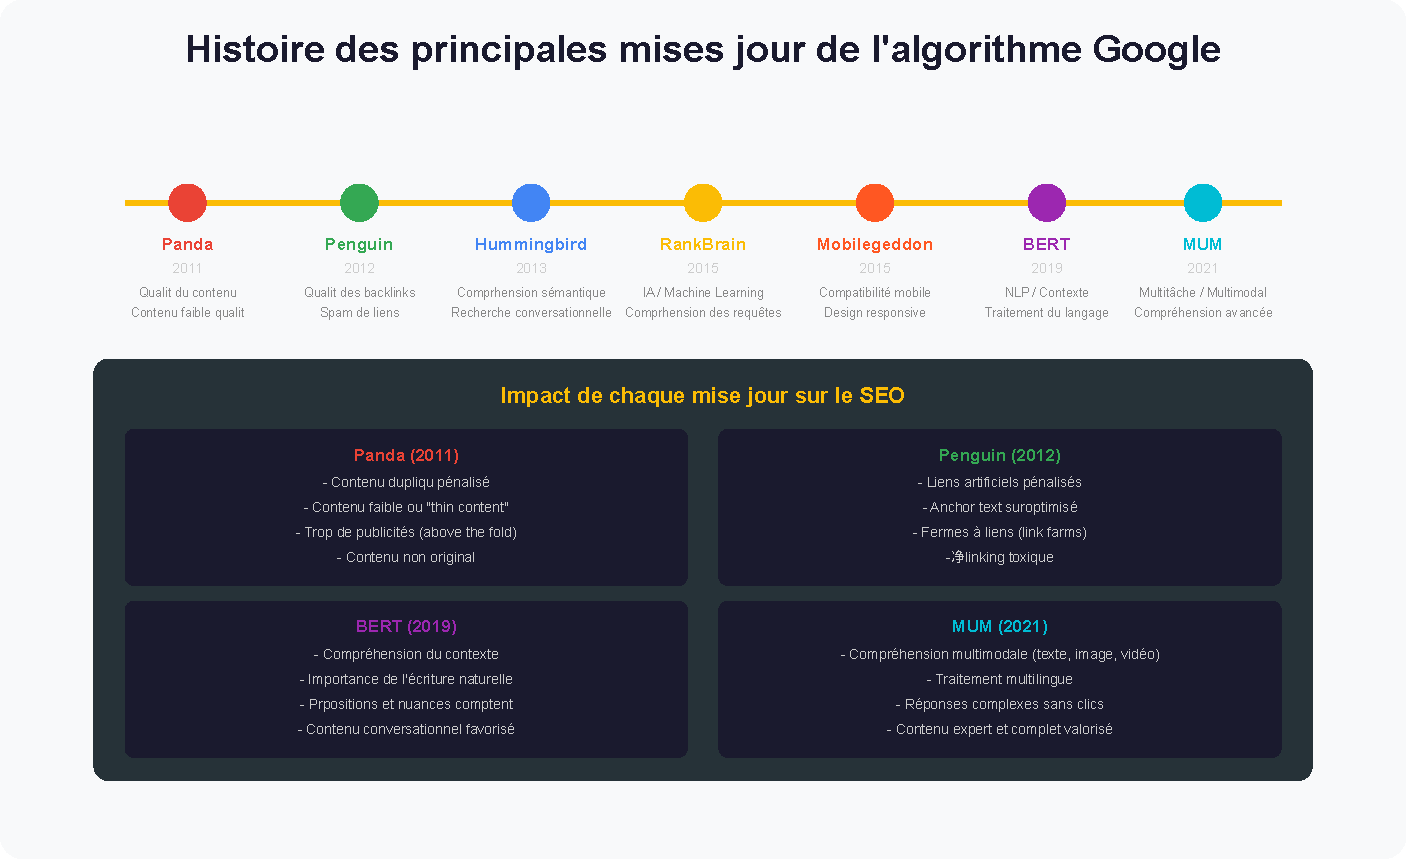
\includegraphics[width=\textwidth]{images/algorithmes_google.pdf}
    \caption{Histoire des principales mises à jour de l'algorithme Google et leur impact sur le SEO}
    \label{fig:algos}
\end{figure}

\section{Les parts de marché des moteurs de recherche}

En 2026, Google domine toujours le marché mondial de la recherche avec environ 91\% de parts de marché, suivi de Bing avec 3,5\%, Baidu (Chine) avec 2,5\%, Yahoo! avec 1,2\% et Yandex (Russie) avec 0,9\%. Cette domination absolue fait de Google le moteur de recherche de référence pour toute stratégie SEO. Historiquement, AltaVista détenait 20\% du marché en 1998 avant d'être supplanté par Google, illustrant la rapidité des transitions dans ce secteur.

\section{Du Web 1.0 au Web 3.0 : l'évolution de la recherche}

La recherche web a suivi l'évolution du web lui-même : le \keyword{Web 1.0} (1990--2005) était un web de documents statiques où la recherche reposait sur des index simples et des annuaires. Le \keyword{Web 2.0} (2005--2020) a introduit le contenu généré par les utilisateurs, les réseaux sociaux et le web dynamique, obligeant les moteurs à intégrer des signaux sociaux. Le \keyword{Web 3.0} (2020--présent) est un web sémantique et décentralisé où l'IA comprend le contexte, les entités et les relations entre concepts bien au-delà des mots-clés.

\section{Étude de cas : évolution du comportement des utilisateurs}

Une étude comparative sur 15 ans montre comment Google a transformé les habitudes de recherche. En 2010, la requête type faisait 2,3 mots en moyenne et 70\% des clics allaient vers les résultats organiques. En 2026, la recherche vocale a allongé la requête moyenne à 4,8 mots, les featured snippets répondent directement à 35\% des requêtes sans clic, et les SERP zero-click représentent 58\% des recherches. Cette évolution a contraint les SEO à optimiser non plus seulement pour le classement mais aussi pour les extraits optimaux et les réponses directes.

% ========== CHAPITRE 2 ==========
\begin{takeaways}
\begin{itemize}
    \item Les moteurs de recherche ont évolué d'annuaires manuels à des systèmes IA complexes
    \item Google a révolutionné la recherche avec l'index inversé et le PageRank
    \item Les mises à jour algorithmiques visent à améliorer la pertinence des résultats
    \item Le métier de SEO a évolué parallèlement aux innovations de Google depuis les années 2000
\end{itemize}
\end{takeaways}

\level{1}
\begin{objectives}
\begin{itemize}
    \item Comprendre les trois étapes fondamentales : crawling, indexation, ranking
    \item Maîtriser le fonctionnement du PageRank
    \item Analyser le pipeline technique d'un moteur de recherche
\end{itemize}
\end{objectives}

\chapter{Fonctionnement technique des moteurs de recherche}
\label{ch:fonctionnement}

\section{Les trois étapes fondamentales}

Le fonctionnement d'un moteur de recherche comme Google repose sur trois étapes critiques et interdépendantes. Comprendre ces mécanismes est essentiel pour tout professionnel du SEO.

\begin{figure}[H]
    \centering
    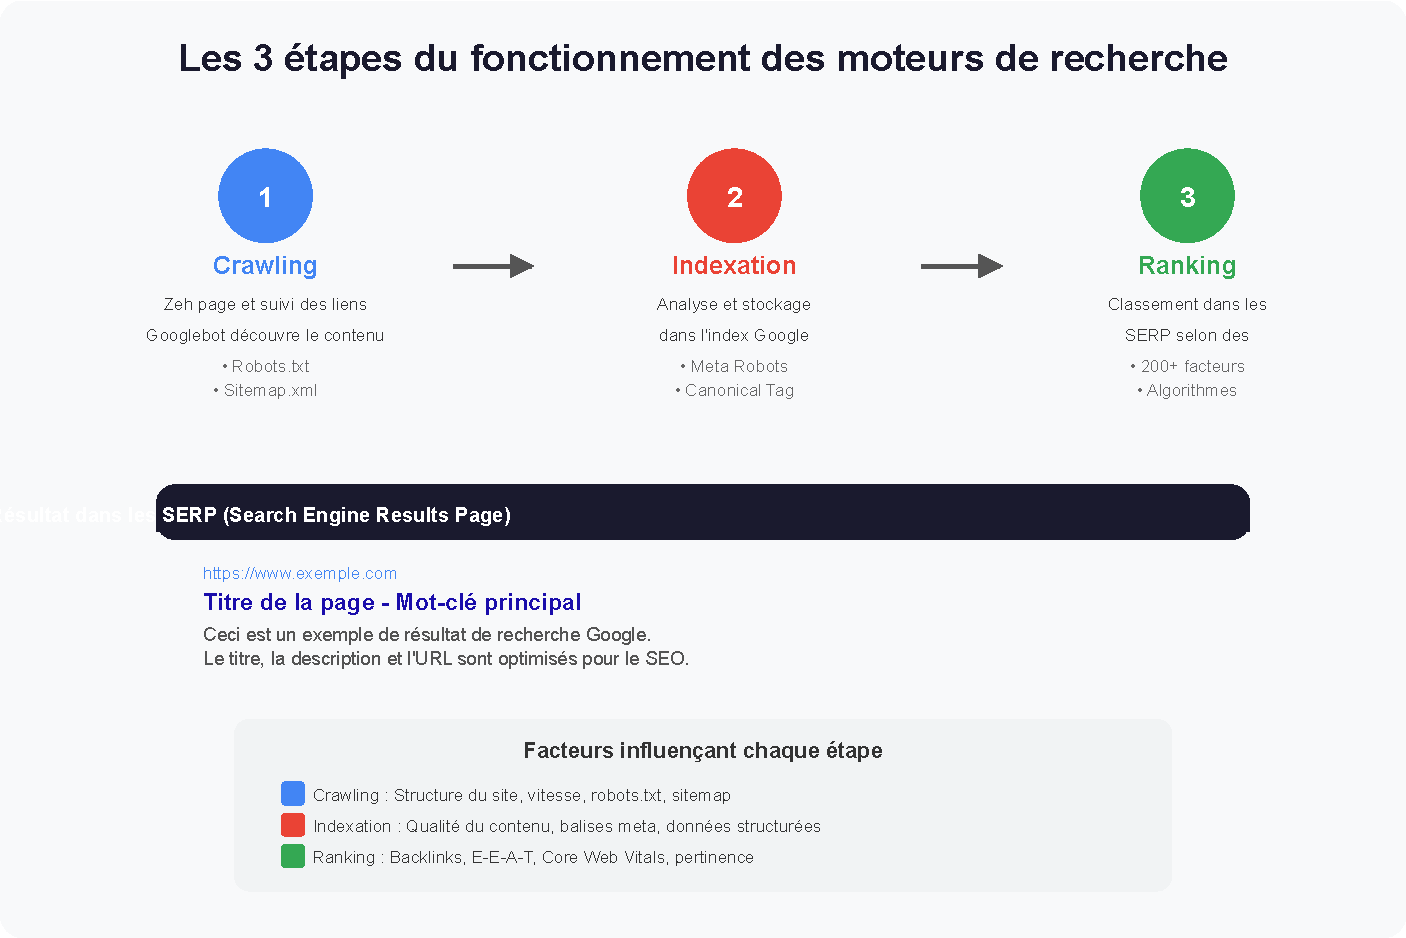
\includegraphics[width=\textwidth]{images/diagramme_moteur_recherche.pdf}
    \caption{Les trois étapes du fonctionnement des moteurs de recherche : Crawling, Indexation, Ranking}
    \label{fig:moteur}
\end{figure}

\begin{figure}[H]
    \centering
    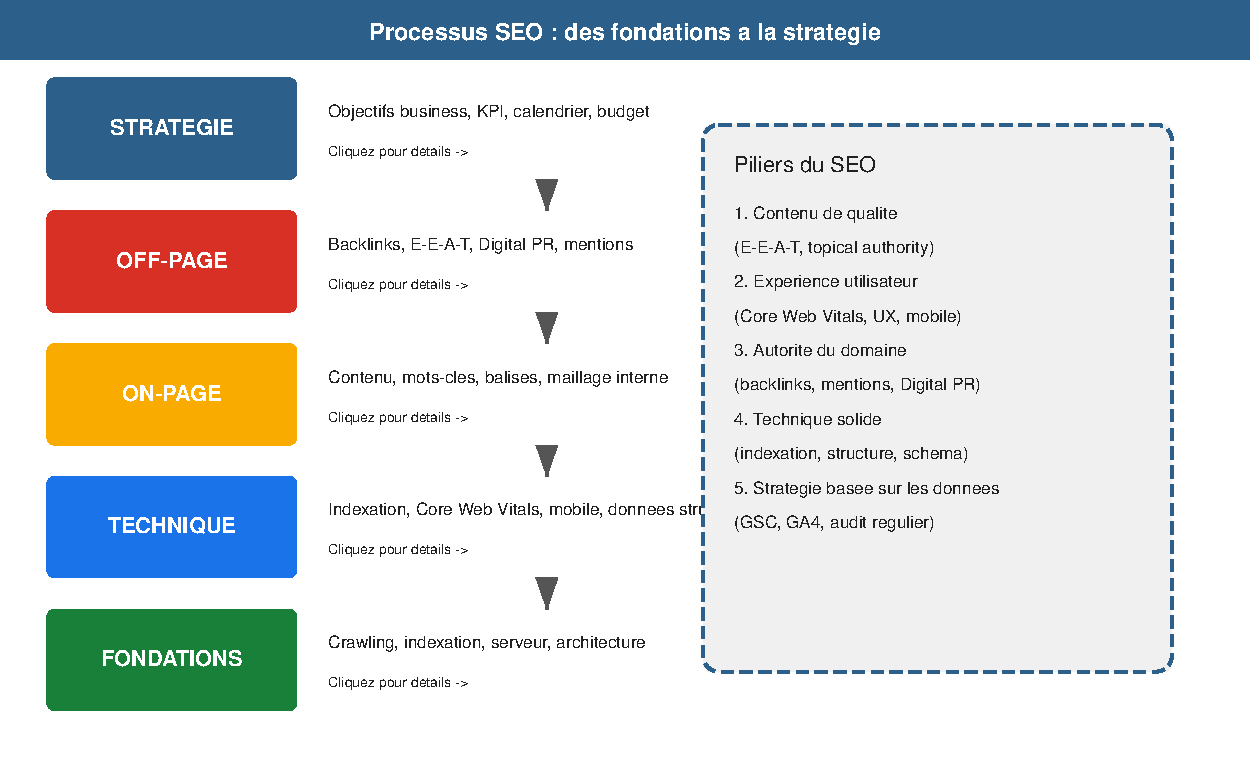
\includegraphics[width=\textwidth]{images/seo_process_overview.pdf}
    \caption{Les cinq piliers du SEO : des fondations techniques à la stratégie}
    \label{fig:seo_overview}
\end{figure}

\subsection{Le crawling (exploration)}

Le \keyword{crawling} est la première étape du processus. Google déploie des robots logiciels appelés \keyword{Googlebot} (ou spiders/crawlers) qui parcourent le web en suivant les liens hypertextes. Ces robots commencent par une liste d'URLs connues, puis extraient les liens de chaque page visitée pour découvrir de nouvelles URLs.

\subsubsection{Le fonctionnement du Googlebot}

Le Googlebot fonctionne en mode asynchrone : il télécharge une page, analyse son contenu HTML, extrait les liens, et les ajoute à une file d'attente priorisée. Plusieurs facteurs déterminent la fréquence de crawl :

\begin{itemize}
    \item La popularité de la page (plus elle reçoit de liens, plus elle est crawlée fréquemment)
    \item La fraîcheur du contenu (les pages mises à jour régulièrement sont revisitée plus souvent)
    \item La vitesse de réponse du serveur (un serveur lent réduit le crawl budget)
    \item La taille du site (les sites vastes nécessitent un budget de crawl plus important)
\end{itemize}

\subsection{L'indexation (stockage et analyse)}

Une fois la page crawlée, Google doit décider si elle mérite d'être intégrée à son index. L'\keyword{indexation} est le processus d'analyse et de stockage des informations contenues dans la page.

\begin{mybox}{Ce que Google analyse lors de l'indexation}{googlegreen}
\begin{itemize}
    \item Le contenu textuel (mots, phrases, structure)
    \item Les balises HTML (title, meta description, headings)
    \item Les attributs des images (alt text, filename)
    \item Les liens (internes et externes)
    \item Les données structurées (Schema.org)
    \item La qualité perçue du contenu
    \item La pertinence par rapport aux requêtes potentielles
\end{itemize}
\end{mybox}

\subsection{Le ranking (classement)}

Le \keyword{ranking} est l'étape finale où Google détermine l'ordre d'affichage des résultats pour une requête donnée. Plus de 200 facteurs de classement sont pris en compte, dont voici les plus importants :

\begin{enumerate}
    \item La pertinence du contenu par rapport à la requête
    \item L'autorité du domaine (basée sur la qualité des backlinks)
    \item L'expérience utilisateur (Core Web Vitals)
    \item La compatibilité mobile
    \item La sécurité (HTTPS)
    \item La fraîcheur du contenu
    \item Les signaux comportementaux (CTR, temps passé)
    \item Les données structurées
    \item E-E-A-T (Experience, Expertise, Authoritativeness, Trustworthiness)
\end{enumerate}

\section{Le PageRank en détail}

Le \keyword{PageRank} est l'algorithme fondateur de Google. Bien qu'il ne soit plus le seul facteur de classement, il reste conceptuellement important. La formule mathématique simplifiée est :

\[
PR(A) = (1-d) + d \sum_{i=1}^{n} \frac{PR(T_i)}{C(T_i)}
\]

Où :
\begin{itemize}
    \item $PR(A)$ est le PageRank de la page A
    \item $d$ est le facteur d'amortissement (généralement 0,85)
    \item $PR(T_i)$ est le PageRank de la page qui pointe vers A
    \item $C(T_i)$ est le nombre de liens sortants de la page $T_i$
\end{itemize}

Cette formule signifie que le PageRank se propage à travers les liens, mais qu'il se dilue à mesure qu'une page a plus de liens sortants.

\begin{figure}[H]
    \centering
    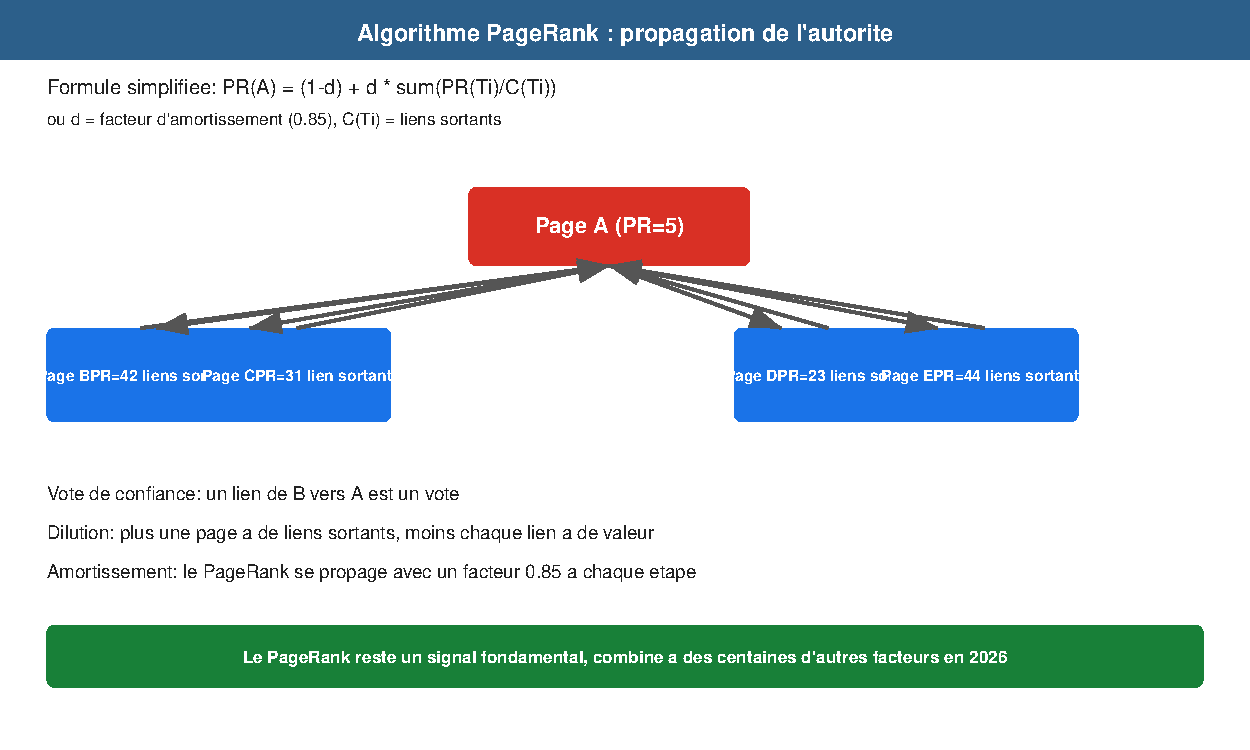
\includegraphics[width=\textwidth]{images/pagerank_flow.pdf}
    \caption{Propagation du PageRank entre les pages : les liens sont des votes de confiance avec facteur d'amortissement de 0,85}
    \label{fig:pagerank}
\end{figure}

% ========== CHAPITRE 3 ==========
\begin{takeaways}
\begin{itemize}
    \item Le crawling explore le web via des robots (Googlebot)
    \item L'indexation organise et stocke les pages dans une base de données
    \item Le ranking classe les résultats selon des centaines de critères
    \item Le PageRank reste un signal fondamental mais n'est plus unique
\end{itemize}
\end{takeaways}

\level{1}
\begin{objectives}
\begin{itemize}
    \item Comprendre le rôle de l'IA dans les moteurs de recherche modernes
    \item Identifier les algorithmes majeurs : RankBrain, BERT, MUM
    \item Analyser l'impact du machine learning sur le classement des résultats
\end{itemize}
\end{objectives}

\chapter{Les moteurs de recherche modernes et l'intelligence artificielle}
\label{ch:ia}

\section{RankBrain : l'apprentissage automatique}

En 2015, Google a introduit \keyword{RankBrain}, un système d'intelligence artificielle basé sur le \keyword{machine learning} qui aide à traiter les résultats de recherche. RankBrain est particulièrement efficace pour comprendre les requêtes jamais vues auparavant (environ 15\% des recherches quotidiennes sont inédites).

\subsection{Fonctionnement interne de RankBrain}

RankBrain utilise un \keyword{word embedding} pour transformer les mots en vecteurs numériques (plongements lexicaux). Chaque mot est converti en un vecteur de 300 à 500 dimensions qui représente sa position dans un espace sémantique. Les mots ayant des significations proches (ex: « voiture », « automobile », « véhicule ») se retrouvent à proximité dans cet espace vectoriel. Cela permet à Google de comprendre qu'une requête jamais vue contenant « acheter auto occasion » est sémantiquement proche d'« achat voiture d'occasion » déjà connue.

\begin{mybox}{Impact sur les SERP}{googleblue}
\begin{itemize}
    \item 15\% des requêtes quotidiennes sont inédites — RankBrain les interprète via similarité vectorielle
    \item Le système apprend en continu des clics des utilisateurs pour affiner ses prédictions
    \item RankBrain est le troisième facteur de classement le plus important selon Google
    \item Il ne remplace pas PageRank mais le complète pour la compréhension sémantique
\end{itemize}
\end{mybox}

\subsection{Implications SEO pratiques}

L'optimisation pour RankBrain ne passe plus par le bourrage de mots-clés mais par une couverture sémantique complète. Un article sur le « SEO technique » doit naturellement inclure des termes associés comme « crawling », « indexation », « Core Web Vitals », « balises canoniques », car Google s'attend à trouver ce champ lexical dans un contenu expert.

\section{BERT : la compréhension du langage naturel}

\keyword{BERT} (Bidirectional Encoder Representations from Transformers) représente une avancée majeure dans la compréhension du langage naturel. Déployé en 2019, BERT a impacté une recherche sur dix, principalement sur les requêtes conversationnelles et les prépositions.

\subsection{L'architecture Transformer}

BERT est basé sur l'architecture \keyword{Transformer}, introduite par Google en 2017 dans l'article \textit{« Attention Is All You Need »}. Le cœur de cette architecture est le mécanisme d'\keyword{attention} multi-tête :

\[
\text{Attention}(Q,K,V) = \text{softmax}\left(\frac{QK^T}{\sqrt{d_k}}\right)V
\]

Où \(Q\) (Query), \(K\) (Key) et \(V\) (Value) sont des matrices représentant les mots de la phrase. Le produit \(QK^T\) calcule le score d'attention entre chaque paire de mots, permettant au modèle de pondérer l'importance de chaque mot pour comprendre le contexte.

Contrairement aux modèles précédents (RNN, LSTM) qui lisaient le texte séquentiellement, BERT lit le texte dans les deux directions simultanément grâce à l'\keyword{attention bidirectionnelle}. Cela lui permet de comprendre qu'une même phrase peut avoir des sens différents selon le contexte.

\subsection{Exemple de compréhension contextuelle}

Considérons la phrase : « Il a ouvert un \textbf{compte} en banque » vs « Il m'a \textbf{compté} une histoire ». BERT comprend que le mot « compte » renvoie à des entités différentes grâce au contexte environnant. Avant BERT, Google pouvait confondre ces deux usages.

\begin{lstlisting}[style=code,caption={Exemple Python : tokenization et attention BERT avec Hugging Face}]
from transformers import BertTokenizer, BertModel
import torch

tokenizer = BertTokenizer.from_pretrained('bert-base-uncased')
model = BertModel.from_pretrained('bert-base-uncased')

phrase = "The bank of the river was beautiful."
inputs = tokenizer(phrase, return_tensors='pt')
outputs = model(**inputs)

# Les embeddings contextuels integrent le sens
# Le mot "bank" est represente differemment
# selon qu'il est suivi de "river" ou "account"
print(outputs.last_hidden_state.shape)
# torch.Size([1, 10, 768])
\end{lstlisting}

\subsection{Impact SEO de BERT}

\begin{itemize}
    \item Les \important{prépositions} et les \important{nuances} comptent désormais : « cours SEO pour débutants » n'est pas équivalent à « cours SEO avancé »
    \item Le \keyword{contenu naturel} est favorisé : les textes qui sonnent artificiels (suroptimisation) sont pénalisés
    \item Les questions longues et conversationnelles (recherche vocale) sont mieux comprises
    \item Les \keyword{featured snippets} ont évolué pour mieux correspondre à l'intention réelle
\end{itemize}

\section{MUM : le modèle multimodal}

\keyword{MUM} (Multitask Unified Model), annoncé en 2021, est 1000 fois plus puissant que BERT avec 1000 milliards de paramètres. Il est fondé sur l'architecture \keyword{T5} (Text-to-Text Transfer Transformer) étendue au traitement multimodal.

\subsection{Architecture et capacités multimodales}

MUM peut comprendre et générer du contenu dans 75 langues et traite simultanément plusieurs formats : texte, images, vidéos et même audio. Sa force réside dans le \keyword{transfert de connaissances} : une information apprise dans une langue peut être utilisée pour répondre à une requête dans une autre langue.

Par exemple, un utilisateur français cherchant « randonnée GR20 » peut recevoir des résultats basés sur des contenus italiens ou anglais évaluant le niveau de difficulté, grâce à la capacité de MUM à comprendre du contenu dans des langues qu'il n'a jamais vues pour cette requête spécifique.

\subsection{Application pratique de MUM}

Google Lens illustre la puissance de MUM : prenez une photo de vos chaussures de randonnée usées, et MUM peut identifier le modèle, trouver des tutoriels vidéo de réparation (en allemand), vérifier la disponibilité en magasin (en polonais), et vous proposer un guide d'achat — le tout sans que vous ayez à formuler chaque étape.

\begin{mybox}{Comparaison des algorithmes d'IA de Google}{teal}
\begin{tabular}{|p{4cm}|p{3.5cm}|p{3.5cm}|p{3.5cm}|}
\hline
\textbf{Critère} & \textbf{RankBrain (2015)} & \textbf{BERT (2019)} & \textbf{MUM (2021)} \\
\hline
Type & ML classique & Transformer bidirectionnel & Transformer multimodal \\
\hline
Paramètres & $\sim$quelques millions & 340 millions & 1000 milliards \\
\hline
Langues & 1 (anglais à l'origine) & 104 & 75 \\
\hline
Modalités & Texte & Texte & Texte, image, vidéo, audio \\
\hline
Fonction & Embedding de requêtes & Compréhension contextuelle & Raisonnement cross-modal \\
\hline
Impact & Requêtes inédites & Nuances/prépositions & Requêtes complexes multi-sources \\
\hline
\end{tabular}
\end{mybox}

\subsection{Implications pour le SEO}

\begin{itemize}
    \item \textbf{RankBrain} : Optimisez pour l'intention en couvrant le champ sémantique complet
    \item \textbf{BERT} : Écrivez naturellement, variez les formulations, soignez les prépositions
    \item \textbf{MUM} : Créez un contenu expert, complet et multimodal (texte + images + vidéos) ; le contenu doit pouvoir répondre à des questions complexes en une seule page
\end{itemize}

\begin{mybox}{Stratégie SEO pour l'ère de l'IA}{googlegreen}
Pour bien se classer dans un moteur de recherche piloté par l'IA :
\begin{enumerate}
    \item Adoptez une approche \keyword{topical authority} : couvrez un sujet en profondeur
    \item Structurez votre contenu avec des \keyword{topical clusters} (pages piliers + pages clusters)
    \item Utilisez un langage \important{naturel} et varié, pas de mots-clés sur-optimisés
    \item Intégrez du contenu \keyword{multimodal} : texte, images optimisées, vidéos, données structurées
    \item Répondez aux \keyword{questions implicites} : anticipez ce que l'utilisateur veut vraiment savoir
    \item Maintenez votre contenu \keyword{à jour} : l'IA valorise la fraîcheur et l'actualité
\end{enumerate}
\end{mybox}

% ============================================
% PARTIE 2 : INDEXATION
% ============================================

\part{L'Indexation -- Le Pilier Technique du Référencement}
\label{part:indexation}

% ========== CHAPITRE 4 ==========
\begin{takeaways}
\begin{itemize}
    \item RankBrain utilise l'apprentissage automatique pour traiter les requêtes nouvelles
    \item BERT permet de comprendre le contexte des mots dans une phrase
    \item MUM est un modèle multimodal qui comprend texte, images et vidéos
\end{itemize}
\end{takeaways}

\level{1}
\begin{objectives}
\begin{itemize}
    \item Maîtriser le pipeline complet d'indexation
    \item Savoir vérifier l'indexation d'un site
    \item Diagnostiquer et résoudre les problèmes d'indexation courants
\end{itemize}
\end{objectives}

\chapter{Le processus d'indexation en profondeur}
\label{ch:indexation}

\section{Les mécanismes d'indexation}

L'indexation est le processus par lequel Google analyse, traite et stocke les pages web dans son index. Ce processus est fondamental : si votre page n'est pas indexée, elle n'existe tout simplement pas dans Google.

\subsection{Le pipeline d'indexation}

Le pipeline d'indexation de Google se déroule en plusieurs phases :

\begin{enumerate}
    \item \textbf{Découverte} : Googlebot trouve une URL via un sitemap, un lien ou une soumission manuelle
    \item \textbf{Téléchargement} : Le robot télécharge la page et ses ressources (CSS, JavaScript, images)
    \item \textbf{Rendu} : Google render la page (exécute le JavaScript) pour voir le contenu final
    \item \textbf{Analyse} : Le contenu est analysé, les liens sont extraits
    \item \textbf{Indexation} : La page est stockée dans l'index si elle répond aux critères de qualité
    \item \textbf{Classification} : La page est catégorisée par thématiques et mots-clés
\end{enumerate}

\section{Comment vérifier l'indexation ?}

Plusieurs méthodes permettent de vérifier si une page est indexée :

\begin{itemize}
    \item Utiliser la commande \texttt{site:votresite.com} dans Google
    \item Consulter le rapport de couverture dans Google Search Console
    \item Utiliser l'outil d'inspection d'URL dans GSC
    \item Vérifier le fichier de logs de votre serveur (présence du Googlebot)
\end{itemize}

\section{Les problèmes d'indexation courants}

\subsection{Les erreurs de crawl}

Le rapport de couverture de Google Search Console révèle plusieurs types d'erreurs :

\begin{itemize}
    \item \important{Erreur 404 (Not Found)} : La page n'existe pas
    \item \important{Erreur 500 (Server Error)} : Le serveur ne répond pas correctement
    \item \important{Erreur de redirection} : Chaîne de redirections trop longue ou boucle
    \item \important{Blocage par robots.txt} : La page est bloquée par le fichier robots.txt
    \item \important{Soft 404} : La page renvoie un statut 200 mais affiche un contenu d'erreur
    \item \important{Orphan pages} : Pages sans aucun lien interne pointant vers elles
\end{itemize}

\subsection{Analyse pratique du rapport Coverage}

Pour analyser le rapport Coverage dans Google Search Console comme un expert :

\begin{enumerate}
    \item Ouvrez Google Search Console et sélectionnez votre site
    \item Allez dans "Indexation" $>$ "Pages" (ou "Coverage")
    \item Analysez les quatre catégories :
    \begin{itemize}
        \item \textbf{Erreur} : Pages qui n'ont pas pu être indexées (à corriger en priorité)
        \item \textbf{Valide avec avertissement} : Pages indexées mais avec des problèmes potentiels
        \item \textbf{Valide} : Pages correctement indexées
        \item \textbf{Exclu} : Pages intentionnellement non indexées (bloquées, canonicalisées, etc.)
    \end{itemize}
    \item Exportez les données pour chaque catégorie et priorisez les corrections
    \item Utilisez l'outil d'inspection d'URL pour des diagnostics détaillés
\end{enumerate}

\subsection{Comment détecter les Orphan Pages}

Les \keyword{orphan pages} sont des pages qui ne sont liées par aucun lien interne. Pour les détecter :

\begin{enumerate}
    \item Utilisez un outil de crawl comme Screaming Frog, Sitebulb ou DeepCrawl
    \item Configurez l'outil avec votre sitemap XML comme point de départ
    \item Identifiez les URLs dans le sitemap qui ne sont pas trouvées par le crawl interne
    \item Vérifiez Google Analytics pour les pages qui reçoivent du trafic mais sans liens internes
    \item Créez des liens internes vers ces pages depuis des pages pertinentes
\end{enumerate}

\subsection{Comment résoudre les Soft 404}

Les \important{Soft 404} sont des pages qui affichent un message d'erreur mais renvoient un code HTTP 200 (OK). Pour les résoudre :

\begin{enumerate}
    \item Identifiez les Soft 404 via le rapport Coverage de GSC
    \item Modifiez le serveur pour renvoyer un véritable statut 404 (\texttt{HTTP/1.1 404 Not Found})
    \item Si la page est supprimée définitivement, utilisez une redirection 301 vers une page pertinente
    \item Personnalisez votre page 404 avec des liens utiles pour l'utilisateur
\end{enumerate}

% ========== CHAPITRE 5 ==========

\begin{exercise}
\begin{enumerate}
    \item Utilisez Google Search Console pour vérifier l'indexation d'un site de votre choix.
    \item Identifiez les pages indexées et celles exclues dans le rapport de couverture.
    \item Repérez au moins 3 problèmes d'indexation et proposez des solutions.
    \item Rédigez un rapport d'analyse de 1 page maximum.
\end{enumerate}
\end{exercise}

\begin{takeaways}
\begin{itemize}
    \item L'indexation suit un pipeline structuré : analyse, extraction, stockage
    \item Les erreurs de crawl et les soft 404 sont des problèmes fréquents
    \item Les pages orphelines ne sont pas crawlées et donc pas indexées
\end{itemize}
\end{takeaways}

\level{2}
\begin{objectives}
\begin{itemize}
    \item Maîtriser la syntaxe et les directives du fichier robots.txt
    \item Savoir créer et optimiser un sitemap XML
    \item Comprendre l'interaction entre robots.txt et sitemap
\end{itemize}
\end{objectives}

\chapter{Le contrôle du crawling : Robots.txt et Sitemap.xml}
\label{ch:controle}

\section{Le fichier robots.txt}

Le fichier \keyword{robots.txt} est un fichier texte placé à la racine du site (\texttt{www.exemple.com/robots.txt}) qui donne des instructions aux robots des moteurs de recherche. C'est le premier fichier que Googlebot consulte avant de crawler un site.

\subsection{Syntaxe et directives avancées}

Au-delà des directives de base \texttt{Disallow} et \texttt{Allow}, le fichier robots.txt supporte des instructions avancées :

\begin{itemize}
    \item \texttt{Crawl-delay} (non supporté par Google mais par Bing et Yandex) : définit le délai en secondes entre deux requêtes du robot 
    \item \texttt{Pattern matching} : utilisation de caractères génériques comme \texttt{*} (n'importe quelle séquence) et \texttt{\$} (fin d'URL)
    \item \texttt{Allow} : utilisé pour créer des exceptions à une règle \texttt{Disallow} (Google traite la règle la plus spécifique comme prioritaire)
\end{itemize}

\begin{lstlisting}[style=htmlcode,caption={Exemple de fichier robots.txt avec directives avancées}]
User-agent: *
Disallow: /wp-admin/
Disallow: /cgi-bin/
Disallow: /tmp/
Disallow: /private/
Disallow: /*?sort=
Disallow: /*?page=
Disallow: /*.pdf$
Allow: /wp-admin/admin-ajax.php
Crawl-delay: 10

Sitemap: https://www.exemple.com/sitemap.xml
Sitemap: https://www.exemple.com/sitemap-news.xml

User-agent: Googlebot-Image
Allow: /images/

User-agent: GPTBot
Disallow: /
\end{lstlisting}

\subsection{Bonnes pratiques avancées et testing}

\begin{figure}[H]
    \centering
    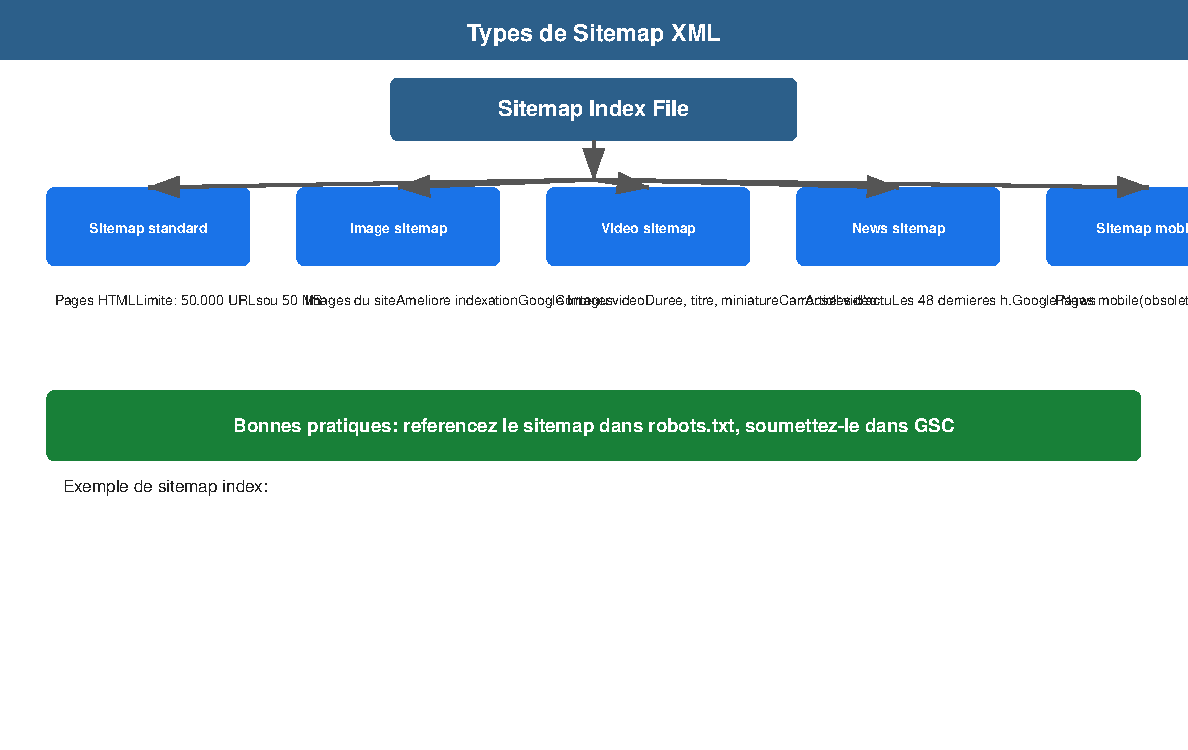
\includegraphics[width=\textwidth]{images/sitemap_types.pdf}
    \caption{Les différents types de sitemap XML : standard, images, vidéos, news}
    \label{fig:sitemap_types}
\end{figure}

\begin{mybox}{Règles d'or pour robots.txt}{googlered}
\begin{itemize}
    \item \important{Ne bloquez jamais les ressources CSS et JavaScript} : Google en a besoin pour le rendu
    \item Utilisez \texttt{Allow} pour des exceptions spécifiques à des règles \texttt{Disallow} larges
    \item Ne tentez pas de cacher du contenu (les concurrents peuvent voir votre robots.txt)
    \item Référencez votre sitemap dans robots.txt
    \item Testez vos directives avec l'outil de test robots.txt dans Google Search Console
    \item Un blocage dans robots.txt empêche le crawling mais pas l'indexation si des liens externes pointent vers la page : utilisez \texttt{noindex} en complément
    \item Utilisez \texttt{User-agent: *} pour les règles générales, puis des \texttt{User-agent} spécifiques pour les exceptions
    \item Les directives pour \texttt{GPTBot} et autres crawlers d'IA sont désormais courantes pour protéger le contenu
\end{itemize}
\end{mybox}

\subsection{Limitation importante : robots.txt et noindex}

\important{Une page bloquée par robots.txt ne peut pas être indexée avec la directive noindex}, car Googlebot ne peut pas télécharger la page pour voir la balise meta robots. Si vous voulez désindexer une page, utilisez \texttt{noindex} sans blocage dans robots.txt. Le blocage dans robots.txt empêche le crawling mais pas l'indexation si des liens externes pointent déjà vers la page.

\section{Le sitemap XML}

Le \keyword{sitemap.xml} est un fichier qui liste toutes les pages importantes d'un site, permettant aux moteurs de recherche de les découvrir rapidement. C'est un complément essentiel au maillage interne, pas un remplacement.

\subsection{Structure du sitemap et optimisations}

\begin{lstlisting}[style=htmlcode,caption={Exemple de sitemap.xml optimisé avec priorités et fréquences}]
<?xml version="1.0" encoding="UTF-8"?>
<urlset xmlns="http://www.sitemaps.org/schemas/sitemap/0.9">
  <url>
    <loc>https://www.exemple.com/</loc>
    <lastmod>2026-06-01</lastmod>
    <changefreq>daily</changefreq>
    <priority>1.0</priority>
  </url>
  <url>
    <loc>https://www.exemple.com/guide-seo</loc>
    <lastmod>2026-05-28</lastmod>
    <changefreq>weekly</changefreq>
    <priority>0.8</priority>
  </url>
</urlset>
\end{lstlisting}

\subsection{Limites et workarounds}

Un sitemap XML ne peut pas dépasser \textbf{50~Mo} (non compressé) ni contenir plus de \textbf{50~000 URLs}. Pour les sites dépassant ces limites, il est nécessaire de créer plusieurs sitemaps reliés par un \keyword{fichier d'index de sitemap} :

\begin{lstlisting}[style=htmlcode,caption={Fichier d'index de sitemap pour grands sites}]
<?xml version="1.0" encoding="UTF-8"?>
<sitemapindex xmlns="http://www.sitemaps.org/schemas/sitemap/0.9">
  <sitemap>
    <loc>https://www.exemple.com/sitemap-produits.xml</loc>
    <lastmod>2026-06-01</lastmod>
  </sitemap>
  <sitemap>
    <loc>https://www.exemple.com/sitemap-articles.xml</loc>
    <lastmod>2026-06-01</lastmod>
  </sitemap>
  <sitemap>
    <loc>https://www.exemple.com/sitemap-categories.xml</loc>
    <lastmod>2026-06-01</lastmod>
  </sitemap>
</sitemapindex>
\end{lstlisting}

\subsection{Stratégie multi-sitemap pour grands sites}

Pour un site de 500~000 pages, la stratégie optimale consiste à organiser les sitemaps par section :
\begin{itemize}
    \item \textbf{sitemap-produits.xml} : Les fiches produits (jusqu'à 50~000 par fichier)
    \item \textbf{sitemap-categories.xml} : Pages de catégories et sous-catégories
    \item \textbf{sitemap-articles.xml} : Contenu éditorial (blog, guides, actualités)
    \item \textbf{sitemap-images.xml} : Images importantes avec leurs métadonnées
    \item \textbf{sitemap-videos.xml} : Contenu vidéo avec durée, miniature, description
\end{itemize}

Chaque sitemap est ensuite référencé dans un unique fichier d'index, lui-même déclaré dans \texttt{robots.txt} et soumis à Google Search Console.

\subsection{Types de sitemaps spécialisés}

Google supporte plusieurs types de sitemaps spécialisés :

\begin{itemize}
    \item \textbf{Sitemap vidéo} (\texttt{<video:video>}) : Pour l'indexation de contenu vidéo avec titre, description, durée, miniature
    \item \textbf{Sitemap images} (\texttt{<image:image>}) : Pour les images avec légende, titre, licence
    \item \textbf{Sitemap actualités} (\texttt{<news:news>}) : Pour les sites d'information, avec date de publication et mot-clé
    \item \textbf{Sitemap mobile} : Pour les pages spécifiques au mobile (obsolète avec le responsive design)
    \item \textbf{Sitemap de géolocalisation} : Pour les sites ayant des adresses physiques
\end{itemize}

\subsection{Cas pratique : optimisation du crawling pour un site média}

Un site d'actualités publie 150 articles par jour et constate que Googlebot ne crawl que 40~\% de ses nouvelles publications. L'audit révèle que le sitemap unique de 80~000 URLs dépasse la limite recommandée en poids. La solution mise en oeuvre comprend : la création de sitemaps quotidiens (\texttt{sitemap-2026-06-01.xml}) chacun contenant les articles du jour, un sitemap index qui référence tous les sitemaps quotidiens, la mise à jour du robots.txt avec \texttt{Crawl-delay} réduit, et l'ajout des balises \texttt{<lastmod>} précises. Résultat : le taux de crawl des nouveaux articles passe à 92~\% en deux semaines.

% ========== CHAPITRE 6 ==========
\begin{takeaways}
\begin{itemize}
    \item robots.txt contrôle l'accès des robots sans bloquer l'indexation
    \item Le sitemap XML guide les moteurs vers les pages importantes
    \item Les sitemaps sont limités à 50~Mo ou 50~000 URLs, nécessitant des fichiers d'index au-delà
    \item Une stratégie multi-sitemap par section optimise la couverture des grands sites
\end{itemize}
\end{takeaways}

\level{2}
\begin{objectives}
\begin{itemize}
    \item Comprendre les directives meta robots et leur impact
    \item Maîtriser l'utilisation du tag canonique
    \item Éviter les erreurs courantes de configuration
\end{itemize}
\end{objectives}

\chapter{Balises Meta Robots et Canonical}
\label{ch:balises}

\section{La balise Meta Robots}

La balise \keyword{meta robots} est une directive insérée dans l'en-tête \texttt{<head>} d'une page HTML qui fournit aux robots des moteurs de recherche des instructions précises sur la manière de traiter cette page. C'est un outil granulaire de contrôle d'indexation.

\subsection{Référence complète des directives}

Google supporte les directives suivantes pour la balise meta robots :

\begin{mybox}{Directives Meta Robots complètes}{googlegreen}
\begin{tabular}{|p{3.5cm}|p{4cm}|p{3.5cm}|p{3cm}|}
\hline
\textbf{Directive} & \textbf{Description} & \textbf{Valeur par défaut} & \textbf{Google} \\
\hline
\texttt{index} & Autoriser l'indexation & index & Oui \\
\hline
\texttt{noindex} & Interdire l'indexation & — & Oui \\
\hline
\texttt{follow} & Suivre les liens & follow & Oui \\
\hline
\texttt{nofollow} & Ne pas suivre les liens & — & Oui \\
\hline
\texttt{noarchive} & Pas de cache Google & — & Oui \\
\hline
\texttt{nosnippet} & Pas d'extrait dans les SERP & — & Oui \\
\hline
\texttt{max-snippet:nombre} & Longueur max de l'extrait & illimité & Oui \\
\hline
\texttt{max-image-preview:taille} & Taille max de l'aperçu image & standard & Oui \\
\hline
\texttt{max-video-preview:secondes} & Durée max aperçu vidéo & illimité & Oui \\
\hline
\texttt{notranslate} & Pas de traduction automatique & — & Oui \\
\hline
\texttt{noimageindex} & Pas d'indexation de l'image & — & Oui \\
\hline
\texttt{unavailable\_after:date} & Ne plus indexer après une date & — & Oui \\
\hline
\texttt{nositelinkssearchbox} & Pas de boîte de recherche site & — & Oui \\
\hline
\end{tabular}
\end{mybox}

\subsection{Exemples avancés de directives combinées}

\begin{lstlisting}[style=htmlcode,caption={Directives Meta Robots avancées}]
<!-- Page d'administration : pas d'indexation, pas de suivi -->
<meta name="robots" content="noindex, nofollow">

<!-- Contenu duplique : indexer mais limiter la preview -->
<meta name="robots" content="index, follow, max-snippet:20,
      max-image-preview:none, max-video-preview:0">

<!-- Contenu temporal : indexer uniquement jusqu'a une date -->
<meta name="robots" content="unavailable_after: 2027-01-01">

<!-- Page de categorie e-commerce : indexer avec preview standard -->
<meta name="robots" content="index, follow, max-image-preview:standard">

<!-- Page avec contenu sensible : pas d'extrait, pas de cache -->
<meta name="robots" content="noarchive, nosnippet">
\end{lstlisting}

\subsection{Directives spécifiques aux robots}

Il est possible de cibler des robots spécifiques avec des directives différentes :

\begin{lstlisting}[style=htmlcode,caption={Directives ciblées par robot}]
<!-- Directive pour Google uniquement -->
<meta name="googlebot" content="noindex, follow">

<!-- Directive pour Bing uniquement -->
<meta name="bingbot" content="noindex">

<!-- Directive generale (tous les robots) -->
<meta name="robots" content="index, follow">

<!-- Directive generale + exception pour Google -->
<meta name="robots" content="index, follow">
<meta name="googlebot" content="nosnippet">
\end{lstlisting}

\subsection{Erreurs fréquentes avec Meta Robots}

\begin{mybox}{Pièges à éviter}{googlered}
\begin{itemize}
    \item \important{Noindex + Disallow dans robots.txt} : Google ne peut pas voir la balise noindex si la page est bloquée dans robots.txt, et l'indexe donc malgré la directive
    \item \important{Directives contradictoires} : \texttt{index, noindex} — Google utilise la directive la plus restrictive
    \item \important{Balise meta robots absente} : Par défaut, tout est \texttt{index, follow}
    \item \important{Multiple balises meta robots} : Google combine les directives (la plus restrictive l'emporte)
    \item \important{X-Robots-Tag} : Pour les fichiers non-HTML (PDF, images), utilisez l'en-tête HTTP \texttt{X-Robots-Tag} plutôt que la balise meta
\end{itemize}
\end{mybox}

\subsection{X-Robots-Tag pour les fichiers non HTML}

Pour contrôler l'indexation de PDF, images ou vidéos :

\begin{lstlisting}[style=code,caption={En-tête HTTP X-Robots-Tag pour les fichiers PDF}]
location ~ \.pdf$ {
    add_header X-Robots-Tag "noindex, noarchive, nosnippet";
}

location ~ \.(mp4|webm|ogg)$ {
    add_header X-Robots-Tag "noindex";
}

location ~ \.(jpg|jpeg|png|gif|webp)$ {
    add_header X-Robots-Tag "index, follow";
}
\end{lstlisting}

\section{Le Tag Canonical}

Le tag \keyword{canonical} (\texttt{rel="canonical"}) est la solution standard pour résoudre les problèmes de contenu dupliqué. Introduit par Google en 2009, il permet d'indiquer au moteur de recherche quelle URL doit être considérée comme la version officielle.

\subsection{Quand utiliser le canonical ?}

\begin{itemize}
    \item \textbf{URLs avec paramètres} : tracking (\texttt{?utm\_source=}), session (\texttt{?sid=}), tri (\texttt{?sort=prix})
    \item \textbf{Contenu syndiqué} : articles republiés sur Medium, LinkedIn, etc.
    \item \textbf{Versions multiples} : imprimable, PDF, AMP
    \item \textbf{Pagination} : page 2, page 3 doivent avoir un canonical auto-référençant
    \item \textbf{HTTP vs HTTPS} : redirection 301 idéale, canonical en renfort
    \item \textbf{www vs non-www} : canonical comme signal complémentaire
    \item \textbf{Pages avec tri différent} : prix, date, popularité — le canonical pointe vers la page par défaut
\end{itemize}

\subsection{Implémentation correcte du canonical}

\begin{lstlisting}[style=htmlcode,caption={Implémentation du tag canonical dans le <head>}]
<!-- Page avec parametres de tracking -->
<link rel="canonical"
      href="https://www.exemple.com/produit/chaise-ergonomique" />

<!-- Auto-canonical (page qui pointe vers elle-meme) -->
<link rel="canonical"
      href="https://www.exemple.com/blog/article-seo" />

<!-- Version syndiquee (pointe vers l'original) -->
<link rel="canonical"
      href="https://www.site-original.fr/article-original" />
\end{lstlisting}

\subsection{Pagination et canonical}

Pour les séries de pages paginées, la gestion du canonical est subtile :

\begin{lstlisting}[style=htmlcode,caption={Canonical pour la pagination}]
<!-- Page 1 : canonical auto-référençant -->
<link rel="canonical"
      href="https://www.exemple.com/categorie/page/1/" />

<!-- Page 2 : canonical auto-référençant ou vers page 1? -->
<!-- Google recommande l'auto-canonical sur chaque page paginee -->
<link rel="canonical"
      href="https://www.exemple.com/categorie/page/2/" />

<!-- Pages 3+ : auto-canonical meme principe -->
<link rel="canonical"
      href="https://www.exemple.com/categorie/page/3/" />

<!-- Avec rel="prev" et rel="next" (aujourd'hui deconseille par Google) -->
<!-- Google ignore desormais prev/next, prefere le canonical -->
\end{lstlisting}

\subsection{Canonical et URLs paramétrées}

Les sites e-commerce sont particulièrement exposés au contenu dupliqué via des paramètres d'URL :

\begin{lstlisting}[style=htmlcode,caption={Gestion des paramètres de filtres e-commerce}]
<!-- URL avec filtre couleur -->
<link rel="canonical"
  href="https://www.exemple.com/chaussures-running" />

<!-- URL avec filtre taille et tri -->
<link rel="canonical"
  href="https://www.exemple.com/chaussures-running" />

<!-- URL de recherche interne -->
<link rel="canonical"
  href="https://www.exemple.com/chaussures-running" />
\end{lstlisting}

\subsection{Bonnes pratiques et erreurs courantes}

\begin{mybox}{Règles d'or du canonical}{googlered}
\begin{itemize}
    \item \important{Le canonical est une suggestion, pas une directive absolue} : Google peut choisir une autre URL si le signal est contradictoire
    \item \important{Toujours utiliser des URLs absolues} : \texttt{https://www.exemple.com/page} et non \texttt{/page}
    \item \important{Éviter les chaînes de canonical} : A pointe vers B qui pointe vers C — Google suit rarement
    \item \important{Canonical auto-référençant} : Chaque page doit avoir un canonical qui pointe vers elle-même même s'il n'y a pas de contenu dupliqué
    \item \important{Ne pas mélanger canonical et noindex} : Si la page est canonicalisée vers une autre, le noindex est inutile
    \item \important{Canonical vers une page 301} : Le canonical doit pointer vers la destination finale de la redirection
    \item \important{Canonical et hreflang} : Le canonical doit pointer vers la même version linguistique que le hreflang correspondant
\end{itemize}
\end{mybox}

\subsection{Exemple complet : site e-commerce avec contenu dupliqué}

\begin{lstlisting}[style=htmlcode,caption={Structure canonical complète pour un site e-commerce}]
<!-- Page produit accessible via plusieurs URLs -->
<!-- URL canonique : /produit/t-shirt-coton-bio -->
<!-- URL alternative 1 : /produit/t-shirt-coton-bio?color=bleu -->
<!-- URL alternative 2 : /produit/t-shirt-coton-bio?size=M -->

<!-- Page officielle -->
<link rel="canonical"
  href="https://example.com/produit/t-shirt-coton-bio" />

<!-- Page fiche produit avec variation couleur -->
<link rel="canonical"
  href="https://example.com/produit/t-shirt-coton-bio" />

<!-- Page avec parametre UTM -->
<link rel="canonical"
  href="https://example.com/produit/t-shirt-coton-bio" />
\end{lstlisting}

\subsection{Cas concret : résolution d'un problème de contenu dupliqué}

\textbf{Scénario :} Un site e-commerce de 10 000 produits voit son contenu dupliqué exploser à cause de 3 paramètres d'URL (couleur, taille, tri). Chaque produit a potentiellement $3 \times 5 \times 4 = 60$ URLs différentes.

\textbf{Solution :}
\begin{enumerate}
    \item Ajouter un \texttt{<link rel="canonical">} sur chaque page produit pointant vers l'URL de base sans paramètres
    \item Configurer Google Search Console pour ignorer les paramètres \texttt{color}, \texttt{size} et \texttt{sort} (Paramètres $\rightarrow$ Paramètres d'URL)
    \item Utiliser des \texttt{fragments} (\texttt{\#}) plutôt que des paramètres (\texttt{?}) pour les variations non essentielles
    \item Ajouter l'attribut \texttt{data-nosnippet} pour les zones de variation dynamique
\end{enumerate}

\textbf{Résultat :} Google consolide les signaux de classement sur l'URL canonique unique, améliorant l'autorité perçue de la fiche produit.

% ========== CHAPITRE 7 ==========
\begin{takeaways}
\begin{itemize}
    \item Les balises meta robots contrôlent l'indexation page par page
    \item Le tag canonical consolide les signaux de pages similaires
    \item L'utilisation incorrecte du canonical peut nuire au référencement
\end{itemize}
\end{takeaways}

\level{2}
\begin{objectives}
\begin{itemize}
    \item Comprendre la notion de budget de crawl
    \item Identifier les facteurs qui influencent le crawl
    \item Optimiser l'allocation du budget de crawl
\end{itemize}
\end{objectives}

\chapter{Le Budget de Crawl (Crawl Budget)}
\label{ch:crawlbudget}

\begin{figure}[H]
    \centering
    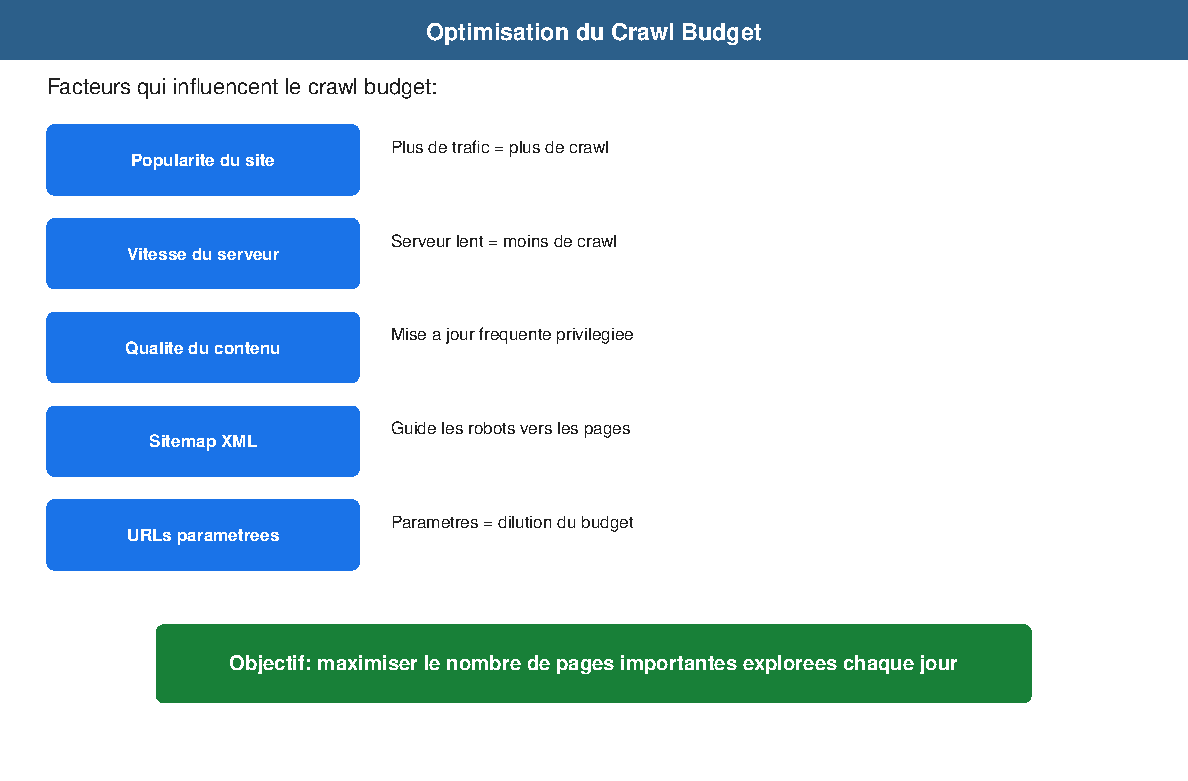
\includegraphics[width=\textwidth]{images/crawl_budget.pdf}
    \caption{Facteurs influençant le crawl budget et stratégies d'optimisation}
    \label{fig:crawl_budget}
\end{figure}

\section{Comprendre le budget de crawl}

Le \keyword{crawl budget} est le nombre de pages que Googlebot va crawler sur votre site dans une période donnée. Ce n'est pas une ressource illimitée, et sa gestion est cruciale pour les sites de grande taille. Google alloue un budget de crawl en fonction de deux paramètres principaux : la \keyword{limite de crawl} (crawl rate limit) et la \keyword{demande de crawl} (crawl demand).

\begin{mybox}{Les deux composantes du crawl budget}{googleblue}
\paragraph{Limite de crawl (Crawl Rate Limit)} Capacité technique maximale de votre serveur à répondre au Googlebot sans surcharge. Si votre serveur répond en moins de 200ms avec des codes 200, Google augmente la cadence. S'il voit des 500 ou des timeouts, il réduit la cadence.

\paragraph{Demande de crawl (Crawl Demand)} Popularité perçue de votre site. Google donne la priorité aux sites qui ont des signaux de qualité forts : backlinks, trafic, fraîcheur du contenu, autorité thématique.
\end{mybox}

\subsection{Facteurs qui influencent le crawl budget}

\begin{mybox}{Facteurs clés du crawl budget}{googleblue}
\begin{itemize}
    \item \textbf{Vitesse du serveur} : Un serveur rapide ($<$ 200ms TTFB) permet plus de crawl
    \item \textbf{Taux d'erreurs} : Trop d'erreurs 404 ou 500 réduisent le budget
    \item \textbf{Popularité} : Les sites populaires reçoivent plus de budget de crawl
    \item \textbf{Fraîcheur du contenu} : Les mises à jour régulières augmentent la fréquence de crawl
    \item \textbf{Qualité du contenu} : Le contenu de faible qualité peut réduire le budget
    \item \textbf{Taille du site} : Les sites plus vastes peuvent obtenir plus de budget (s'ils sont de qualité)
    \item \textbf{Structure des liens} : Un maillage interne dense et cohérent facilite le crawl
    \item \textbf{Présence de sitemap} : Un sitemap XML à jour accélère la découverte de pages
\end{itemize}
\end{mybox}

\section{Surveiller le crawl budget dans Google Search Console}

Google Search Console fournit des outils pour analyser l'activité de crawl :

\begin{enumerate}
    \item \textbf{Rapport Statistiques de crawl} (Paramètres $\rightarrow$ Statistiques de crawl) : Nombre total de requêtes, temps de téléchargement, taille des fichiers
    \item \textbf{Rapport de couverture} (Indexation $\rightarrow$ Pages) : Pages valides, erreurs, exclues
    \item \textbf{Cartographie des paramètres d'URL} (Paramètres $\rightarrow$ Paramètres d'URL) : Indiquez à Google quels paramètres ignorer
\end{enumerate}

\begin{mybox}{Métriques clés dans le rapport de crawl}{googlegreen}
\begin{tabular}{|p{5cm}|p{4cm}|p{4cm}|}
\hline
\textbf{Métrique} & \textbf{Bon signe} & \textbf{Mauvais signe} \\
\hline
Requêtes totales/jour & Stable ou en hausse & Chute brutale \\
\hline
Temps de téléchargement & $<$ 200ms & $>$ 500ms \\
\hline
Taux de réponse 200 & $>$ 95\% & $<$ 90\% \\
\hline
Taux d'erreurs (4xx/5xx) & $<$ 1\% & $>$ 5\% \\
\hline
Pages indexées & Croissance régulière & Stagnation ou baisse \\
\hline
\end{tabular}
\end{mybox}

\section{Optimiser le crawl budget}

\subsection{Actions prioritaires}

\begin{enumerate}
    \item \textbf{Éliminez les pages de faible valeur} : Utilisez \texttt{noindex} pour les pages d'administration, pages de recherche interne, archives de tags, pages de filtre sans contenu unique
    \item \textbf{Optimisez la structure des liens internes} : Les pages importantes doivent être à 1--2 clics de la racine
    \item \textbf{Réduisez les redirections en chaîne} : Chaque redirection consomme du budget
    \item \textbf{Utilisez le paramètre \texttt{noindex} pour les pages non essentielles}
    \item \textbf{Corrigez les erreurs 4xx et 5xx rapidement} : Utilisez le rapport de couverture de GSC
    \item \textbf{Améliorez la vitesse de votre serveur} : Cache, CDN, optimisation applicative
    \item \textbf{Consolidez le contenu dupliqué} via le tag canonical
    \item \textbf{Optimisez votre sitemap XML} : Incluez uniquement les pages importantes (max 50 000 URLs ou 50 Mo)
\end{enumerate}

\subsection{Rôle du robots.txt et du sitemap}

Le fichier \keyword{robots.txt} et le \keyword{sitemap XML} interagissent directement avec le crawl budget :

\begin{itemize}
    \item \textbf{robots.txt} : Bloquez les sections inutiles (administration, scripts, API) pour concentrer le budget sur le contenu utile. Ne bloquez jamais les ressources CSS/JS nécessaires au rendu
    \item \textbf{Sitemap XML} : Guide Google vers les pages prioritaires. Un sitemap bien structuré avec des \texttt{<lastmod>} à jour signale à Google les pages modifiées à recrawler
    \item \textbf{Synchronisation} : Les URLs dans le sitemap doivent être accessibles (pas de 404, pas de redirection, pas de noindex)
\end{itemize}

\section{Analyse des logs serveur pour le crawl budget}

L'analyse des logs serveur est la méthode la plus fiable pour comprendre comment Googlebot se comporte sur votre site.

\subsection{Que rechercher dans les logs}

\begin{enumerate}
    \item \textbf{Fréquence de visite} : À quelle fréquence Googlebot revient-il ?
    \item \textbf{Temps passé} : Combien de temps Google passe-t-il sur chaque page ?
    \item \textbf{Ressources téléchargées} : Quels fichiers CSS, JS, images Google charge-t-il ?
    \item \textbf{Pages ignorées} : Quelles pages importantes Google ne visite-t-il jamais ?
    \item \textbf{Statuts HTTP} : Distribution des codes 200, 301, 404, 500
    \item \textbf{User-Agent} : Googlebot Desktop vs Googlebot Mobile
\end{enumerate}

\begin{lstlisting}[style=code,caption={Script Python pour analyser le comportement de Googlebot dans les logs}]
import re
from collections import Counter
from datetime import datetime

LOG_PATTERN = re.compile(
    r'(?P<ip>\d+\.\d+\.\d+\.\d+)\s+.*\[(?P<date>[^\]]+)\]'
    r'\s+"(?P<method>\w+)\s+(?P<url>\S+)\s+\S+"\s+'
    r'(?P<status>\d+)\s+(?P<size>\d+)'
)

GOOGLEBOT_IPS = [
    '66.249.', '72.14.', '203.208.',
    '216.239.', '209.85.'
]

def parse_log_line(line):
    return LOG_PATTERN.match(line)

def is_googlebot(ip):
    return any(ip.startswith(p) for p in GOOGLEBOT_IPS)

def analyze_logs(logfile):
    pages = Counter()
    statuses = Counter()
    total_requests = 0

    with open(logfile, 'r') as f:
        for line in f:
            match = parse_log_line(line)
            if not match:
                continue

            ip = match.group('ip')
            if not is_googlebot(ip):
                continue

            total_requests += 1
            url = match.group('url')
            status = match.group('status')
            pages[url] += 1
            statuses[status] += 1

    print(f"Requetes Googlebot : {total_requests}")
    print(f"Pages uniques crawlées : {len(pages)}")
    print(f"Top 10 pages :")
    for url, count in pages.most_common(10):
        print(f"  {url} : {count} fois")
    print(f"Distribution des statuts :")
    for status, count in statuses.most_common():
        print(f"  HTTP {status} : {count} ({count/total_requests*100:.1f}%)")

analyze_logs('/var/log/nginx/access.log')
\end{lstlisting}

\section{Étude de cas : optimisation du crawl budget}

\subsection{Scénario : site e-commerce de 100 000 pages}

\textbf{Problème :} Un site e-commerce avec 100 000 pages produits reçoit Googlebot 500 fois par jour. Seulement 30\% des pages importantes sont crawlées régulièrement. Le budget de crawl est gaspillé sur :

\begin{itemize}
    \item 15 000 pages de filtres (couleur, taille, prix) sans contenu unique
    \item 8 000 pages de recherche interne avec paramètres
    \item 5 000 pages d'administration accessibles accidentellement
    \item 2 000 pages de variation de tri (prix croissant, décroissant, etc.)
\end{itemize}

\textbf{Solution mise en oeuvre :}
\begin{enumerate}
    \item Blocage de 25 000 pages inutiles via \texttt{robots.txt} (filtres, recherche interne)
    \item Ajout de \texttt{<meta name="robots" content="noindex">} sur 2 000 pages d'administration
    \item Canonicalisation de 2 000 pages de tri vers la page de catégorie principale
    \item Optimisation du sitemap XML (suppression des pages exclues)
    \item Amélioration du temps de réponse serveur (600ms $\rightarrow$ 180ms via cache Redis + CDN)
\end{enumerate}

\textbf{Résultats après 3 mois :}

\begin{mybox}{Résultats de l'optimisation}{googlegreen}
\begin{tabular}{|p{5cm}|p{3cm}|p{3cm}|p{3cm}|}
\hline
\textbf{Métrique} & \textbf{Avant} & \textbf{Après} & \textbf{Évolution} \\
\hline
Pages crawlées/jour & 500 & 1 200 & +140\% \\
\hline
Pages importantes crawlées & 30\% & 85\% & +183\% \\
\hline
Pages indexées & 45 000 & 72 000 & +60\% \\
\hline
Trafic organique & 120 000 visites/mois & 195 000 visites/mois & +62\% \\
\hline
Erreurs 404 & 8\% & 1,2\% & -85\% \\
\hline
Temps réponse serveur & 600ms & 180ms & -70\% \\
\hline
\end{tabular}
\end{mybox}

\section{Bonnes pratiques pour maximiser le crawl budget}

\begin{enumerate}
    \item \textbf{Mettez à jour votre sitemap} à chaque nouvelle publication (ou au moins quotidiennement)
    \item \textbf{Surveillez le rapport de crawl} dans GSC chaque semaine
    \item \textbf{Utilisez l'inspection d'URL} pour vérifier la dernière date de crawl d'une page importante
    \item \textbf{Soumettez les URLs critiques} via la soumission manuelle dans GSC après une mise à jour majeure
    \item \textbf{Évitez les pages orphelines} : chaque page importante doit avoir au moins un lien interne
    \item \textbf{Gérez les paramètres d'URL} dans GSC pour les sites e-commerce
    \item \textbf{Utilisez \texttt{lastmod}} dans le sitemap pour signaler les pages modifiées
    \item \textbf{Surveillez le fichier de logs} pour détecter les anomalies de crawl
\end{enumerate}

\begin{mybox}{À retenir}{googlered}
Le crawl budget n'est un problème que pour les sites de plus de 10 000 pages. Pour les petits sites, Google crawl généralement toutes les pages sans difficulté. Concentrez vos efforts sur la qualité du contenu et la performance technique avant d'optimiser le crawl budget.
\end{mybox}

% ============================================
% PARTIE 3 : SEO ON-PAGE
% ============================================

\part{Le SEO On-Page -- Optimisation du Contenu}
\label{part:onpage}

\begin{figure}[H]
    \centering
    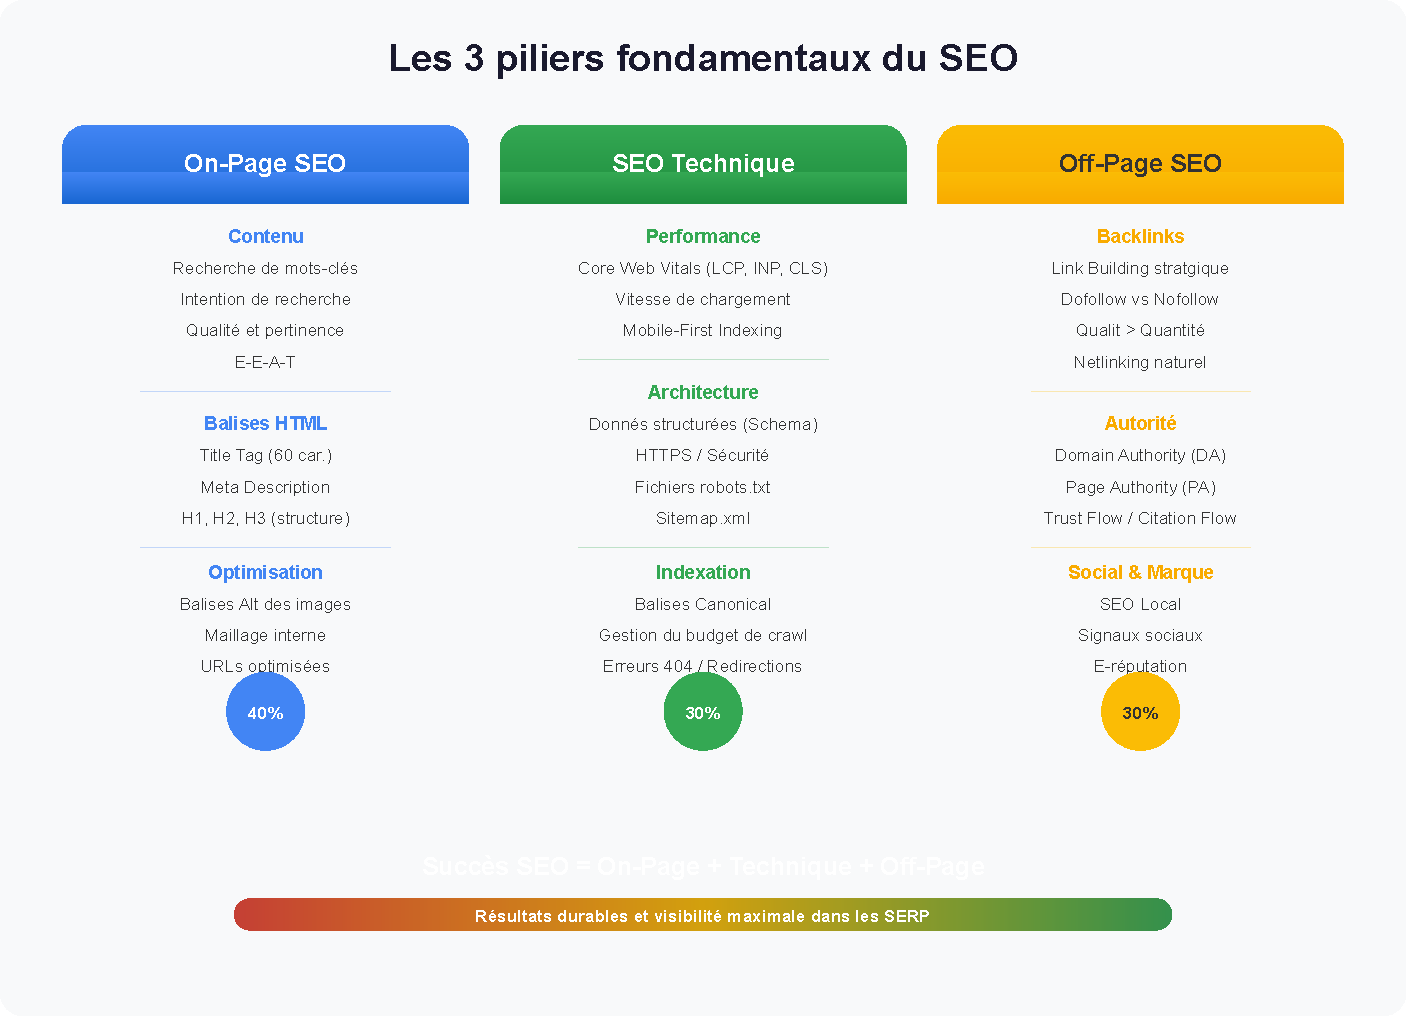
\includegraphics[width=\textwidth]{images/piliers_seo.pdf}
    \caption{Les trois piliers fondamentaux du SEO : On-Page, Technique et Off-Page}
    \label{fig:piliers}
\end{figure}

% ========== CHAPITRE 8 ==========
\begin{takeaways}
\begin{itemize}
    \item Le budget de crawl est le nombre de pages que Google explore par période
    \item La qualité et la popularité du site influencent le budget de crawl
    \item L'optimisation passe par la suppression du contenu de faible valeur
\end{itemize}
\end{takeaways}

\level{1}
\begin{objectives}
\begin{itemize}
    \item Maîtriser les fondamentaux de la recherche de mots-clés
    \item Savoir utiliser les outils professionnels de keyword research
    \item Analyser les métriques essentielles : volume, difficulté, CPC
\end{itemize}
\end{objectives}

\chapter{La recherche de mots-clés (Keyword Research)}
\label{ch:keywords}

\begin{figure}[H]
    \centering
    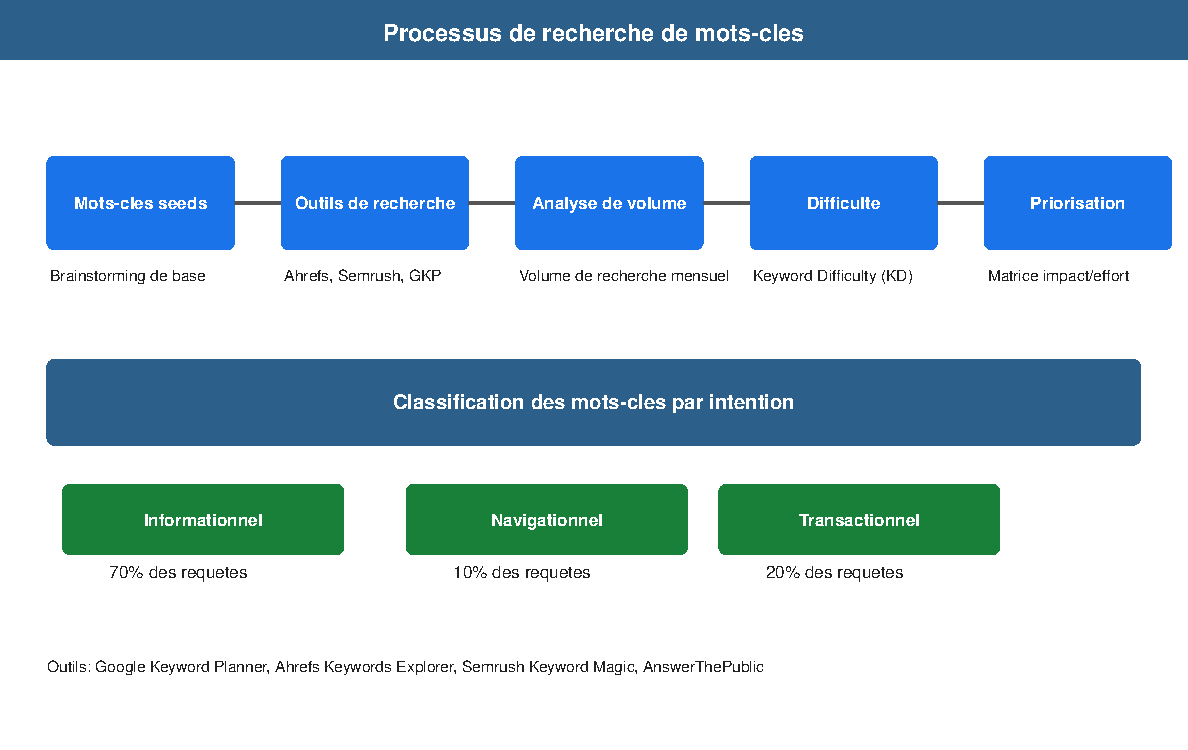
\includegraphics[width=\textwidth]{images/keyword_research.pdf}
    \caption{Processus complet de recherche de mots-clés : des seeds à la priorisation}
    \label{fig:keyword_research}
\end{figure}

\section{Les fondamentaux de la recherche de mots-clés}

La \keyword{recherche de mots-clés} est le point de départ de toute stratégie SEO. Elle consiste à identifier les termes et expressions que votre public cible utilise dans les moteurs de recherche. Une recherche mal exécutée conduit à un contenu non pertinent, un mauvais ciblage et un gaspillage de ressources.

\subsection{Mots-clés seed et expansion sémantique}

Le processus débute par l'identification des \keyword{mots-clés seed} (ou germes) : une liste de 5 à 10 termes représentant le cœur de votre activité. Par exemple, pour un site e-commerce de matériel de randonnée : \texttt{randonnée}, \texttt{sac à dos}, \texttt{chaussures de randonnée}, \texttt{tente}, \texttt{camping}. Ces seeds sont ensuite expansés à l'aide d'outils spécialisés qui suggèrent des variantes, des requêtes associées et des questions fréquentes.

\subsection{Typologie des mots-clés}

\begin{itemize}
    \item \textbf{Short-tail (tête large)} : 1--2 mots, volume élevé, concurrence forte, intention vague
    \begin{itemize}
        \item Exemple : \texttt{chaussures}, \texttt{SEO}, \texttt{formation}
        \item Utile pour la notoriété, difficile à positionner sans autorité
    \end{itemize}
    \item \textbf{Middle-tail} : 2--3 mots, volume modéré, concurrence moyenne
    \begin{itemize}
        \item Exemple : \texttt{chaussures de running}, \texttt{formation SEO Paris}
        \item Bon équilibre entre volume et faisabilité
    \end{itemize}
    \item \textbf{Long-tail (queue longue)} : 3+ mots, volume faible, concurrence faible, intention précise
    \begin{itemize}
        \item Exemple : \texttt{meilleures chaussures de running pour marathon 2026}
        \item Taux de conversion élevé car l'intention est claire
    \end{itemize}
\end{itemize}

\section{Méthodologie complète de recherche}

\subsection{Étape 1 : Constitution du corpus de seeds}

Utilisez plusieurs sources pour générer vos seeds : brainstorming d'équipe, analyse des concurrents (avec des outils comme SEMrush Domain Analytics ou Ahrefs Site Explorer), Google Search Console (requêtes existantes générant des impressions), et suggestions de recherche Google (autocomplete).

\subsection{Étape 2 : Expansion et collecte de données}

Importez vos seeds dans un outil de recherche de mots-clés. Pour chaque terme, collectez :

\begin{itemize}
    \item Le volume de recherche mensuel moyen
    \item La \keyword{difficulté du mot-clé} (KD score, de 0 à 100)
    \item Le coût par clic (CPC) indicatif
    \item Le potentiel de trafic (somme des clics estimés pour les 10 premières positions)
    \item La tendance saisonnière (via Google Trends ou l'historique de l'outil)
\end{itemize}

\subsection{Étape 3 : Analyse de la difficulté et de la concurrence}

La \keyword{difficulté du mot-clé} est une estimation algorithmique fournie par des outils comme Ahrefs ou SEMrush. Elle se base sur la puissance des domaines déjà classés dans le top 10 (nombre de backlinks, Domain Rating, autorité de page). Un KD inférieur à 30 est considéré comme accessible pour un site jeune ; entre 30 et 60 nécessite une stratégie de contenu solide ; au-delà de 60, seuls les sites établis peuvent espérer se classer.

\important{Ne vous fiez pas uniquement au KD : examinez manuellement les résultats SERP. Une page de forum classée pour un mot-clé commercial signale une faible concurrence et une opportunité.}

\subsection{Étape 4 : Clustering et regroupement thématique}

Le \keyword{clustering} consiste à regrouper les mots-clés sémantiquement proches pour créer des pages uniques couvrant un sujet complet plutôt que de multiplier les pages pour chaque variante. Par exemple, les requêtes \texttt{formation SEO en ligne}, \texttt{cours SEO débutant} et \texttt{apprendre le SEO gratuitement} peuvent être traitées sur une même page pilier. Un cluster typique comprend une page pilier (sujet large) et plusieurs articles satellites (sous-thèmes spécifiques).

\subsection{Étape 5 : Matrice de priorisation}

Une fois les données collectées, construisez une \keyword{matrice de priorisation} pour décider quels mots-clés cibler en premier :

\begin{itemize}
    \item \textbf{Quick wins} : KD faible, volume moyen, intention claire --- à traiter en priorité
    \item \textbf{Contenu pilier} : Volume élevé, KD modéré --- nécessite une stratégie de liens
    \item \textbf{Longue traîne} : Volume faible, KD très faible, fort taux de conversion
    \item \textbf{Marque/notoriété} : Volume élevé, KD très élevé --- à long terme
\end{itemize}

\section{Outils de recherche de mots-clés}

\begin{mybox}{Outils recommandés}{googlegreen}
\begin{itemize}
    \item \textbf{Gratuits} : Google Keyword Planner, Google Trends, AnswerThePublic, AlsoAsked (version gratuite limitée), Ubersuggest (version limitée), Keyword Sheeter
    \item \textbf{Payants} : Ahrefs Keywords Explorer (\$99/mois), SEMrush Keyword Magic Tool (\$119/mois), Moz Keyword Explorer, KWFinder (\$49/mois), KWFinder par Mangools
    \item \textbf{Spécialisés} : AlsoAsked (questions associées à partir d'un mot-clé), KeywordTool.io (suggestions depuis plusieurs moteurs), SE Ranking (analyse concurrentielle), Surfer SEO (optimisation sémantique)
\end{itemize}
\end{mybox}

\section{Analyse de la saisonnalité et des tendances}

De nombreux mots-clés subissent des variations saisonnières significatives. Par exemple, \texttt{acheter manteau d'hiver} culmine en octobre--novembre, tandis que \texttt{location vacances été} atteint son pic en janvier--février (réservations anticipées). Utilisez \keyword{Google Trends} pour visualiser ces tendances sur 12 mois et ajustez votre calendrier éditorial en conséquence. Ignorer la saisonnalité conduit à publier un contenu au mauvais moment et à sous-estimer le potentiel réel d'un mot-clé.

\section{Cas pratique : Projet de recherche de mots-clés}

Prenons l'exemple d'un site de commerce électronique spécialisé dans le café artisanal. La liste seed initiale est : \texttt{café}, \texttt{café en grain}, \texttt{machine à café}, \texttt{cafetière}, \texttt{café bio}. L'expansion via Ahrefs génère 485 mots-clés. Après filtrage (volume $>$ 50, pertinence confirmée), il en reste 134. Le clustering réduit ce nombre à 22 pages potentielles réparties en 4 piliers : guide d'achat, préparation, dégustation, et équipement. La priorisation identifie 8 quick wins (KD $<$ 30, volume 200--800) qui constitueront les premiers articles du blog.

\begin{exercise}[Étude de mots-clés]
\begin{enumerate}
    \item Choisissez un domaine qui vous intéresse (voyage, sport, cuisine, technologie...).
    \item Utilisez Google Keyword Planner ou un outil gratuit (Ubersuggest) pour trouver 15 mots-clés seeds.
    \item Exportez les données : volume, KD, CPC, tendance.
    \item Regroupez les mots-clés en clusters thématiques (3 à 5 clusters).
    \item Construisez une matrice de priorisation et identifiez 3 quick wins.
    \item Proposez une stratégie de contenu basée sur ces clusters (pages piliers, articles satellites).
\end{enumerate}
\end{exercise}

\begin{takeaways}
\begin{itemize}
    \item La recherche de mots-clés est la fondation de toute stratégie SEO
    \item Il faut distinguer tête de réseau, corps et longue traîne
    \item Les outils comme SEMrush et Ahrefs fournissent des données essentielles
    \item Le clustering permet d'éviter la cannibalisation et de structurer le contenu
    \item La matrice de priorisation guide l'allocation des ressources
\end{itemize}
\end{takeaways}

\level{1}
\begin{objectives}
\begin{itemize}
    \item Comprendre les quatre types d'intention de recherche
    \item Associer le contenu à l'intention utilisateur
    \item Cartographier le parcours utilisateur complet
\end{itemize}
\end{objectives}

\chapter{L'intention de recherche (Search Intent)}
\label{ch:intent}

\section{L'importance de l'intention}

Depuis l'introduction de \keyword{BERT} (2019) et de \keyword{MUM} (2021), Google accorde une importance capitale à l'\keyword{intention de recherche} (Search Intent). Ces modèles de traitement du langage naturel permettent à Google de comprendre le sens profond d'une requête plutôt que de se limiter à une correspondance mot à mot. Comprendre et satisfaire l'intention est désormais plus important que le simple ciblage de mots-clés.

\begin{figure}[H]
    \centering
    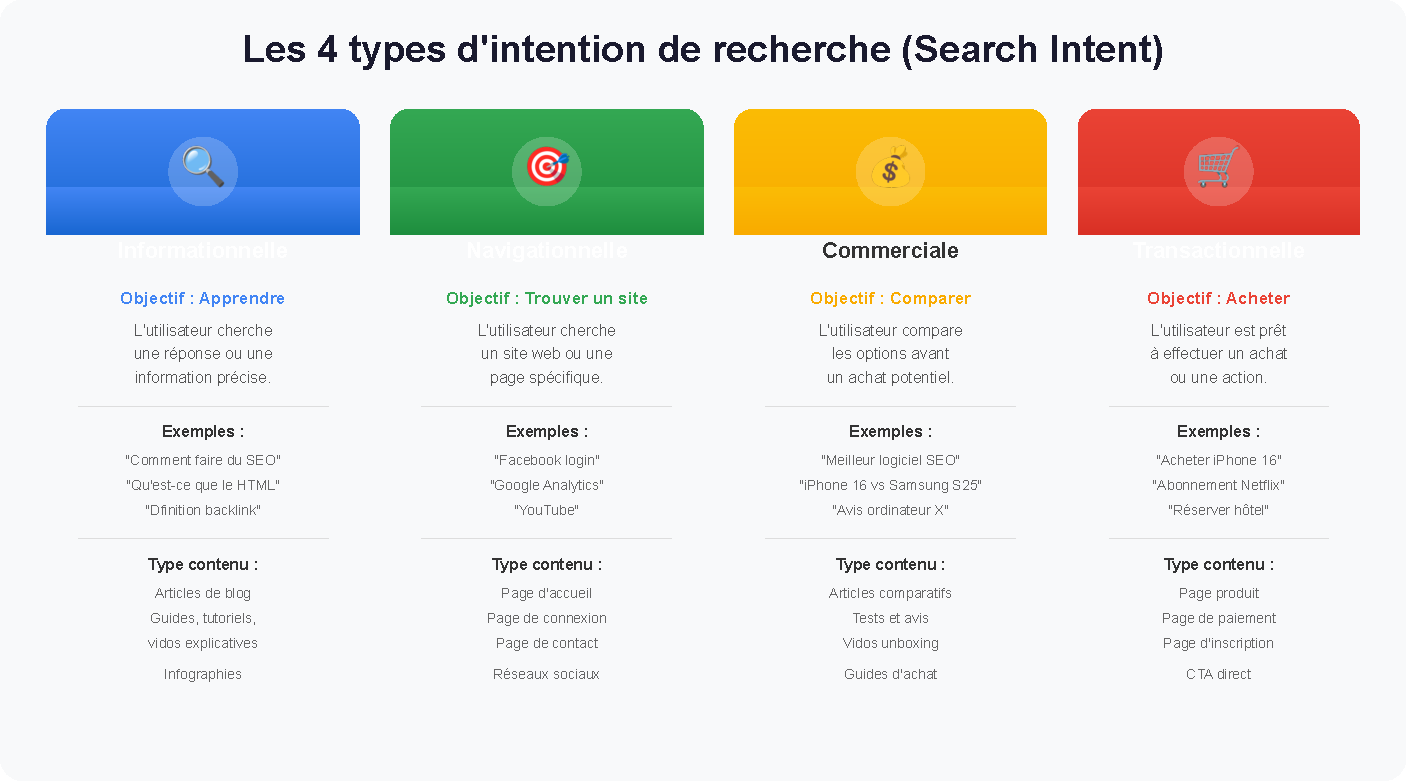
\includegraphics[width=\textwidth]{images/intention_recherche.pdf}
    \caption{Les quatre types d'intention de recherche : Informationnelle, Navigationnelle, Commerciale, Transactionnelle}
    \label{fig:intent}
\end{figure}

\section{Les 4 types d'intention de recherche}

\subsection{Intention informationnelle}
L'utilisateur cherche à apprendre, à comprendre ou à trouver une réponse à une question précise. Exemple : \texttt{Comment faire du SEO ?} ou \texttt{Qu'est-ce que le référencement naturel ?}

\begin{itemize}
    \item \textbf{Contenu adapté} : Articles de blog, guides complets, tutoriels pas à pas, vidéos explicatives, infographies, FAQ, glossaires
    \item \textbf{Format recommandé} : Article long format (1500--3000 mots), structure en questions-réponses, guide illustré
    \item \textbf{SERP Features associées} : Featured snippets (extraits optimaux), Knowledge Panel, People Also Ask, vidéos
    \item \textbf{Stratégie} : Créer le contenu le plus complet possible sur le sujet ; viser le \keyword{featured snippet} en répondant directement à la question dans les 50 premiers mots
\end{itemize}

\subsection{Intention navigationnelle}
L'utilisateur cherche un site web ou une page spécifique dont il connaît déjà l'existence. Exemple : \texttt{Facebook login}, \texttt{Google Analytics console}, \texttt{Amazon retour}.

\begin{itemize}
    \item \textbf{Contenu adapté} : Page d'accueil, page de connexion, page de contact, page de marque
    \item \textbf{Objectif} : Être présent dans le top 3 pour les recherches de marque ; protéger sa e-réputation
    \item \textbf{SERP Features} : Site links (liens supplémentaires sous le résultat principal), Knowledge Panel
    \item \textbf{Stratégie} : Optimiser les pages de marque ; surveiller les requêtes navigationnelles concurrentes
\end{itemize}

\subsection{Intention commerciale}
L'utilisateur compare les options, évalue les alternatives et recherche des avis avant de prendre une décision d'achat. Exemple : \texttt{Meilleur logiciel SEO 2026}, \texttt{iPhone 16 Pro vs Samsung Galaxy S25}.

\begin{itemize}
    \item \textbf{Contenu adapté} : Articles comparatifs, tests et avis détaillés, guides d'achat, vidéos de démonstration, études de cas
    \item \textbf{Format recommandé} : Tableaux comparatifs, listes avec notes, vidéos de test, témoignages clients
    \item \textbf{SERP Features} : Shopping ads, évaluations produits (stars), vidéos, comparaison de produits
    \item \textbf{Stratégie} : Inclure des données chiffrées objectives ; mettre en avant les avantages et inconvénients ; intégrer des CTA vers les pages produits
\end{itemize}

\subsection{Intention transactionnelle}
L'utilisateur est prêt à acheter, à s'inscrire ou à effectuer une action concrète. Exemple : \texttt{Acheter iPhone 16 Pro pas cher}, \texttt{s'abonner newsletter SEO}, \texttt{télécharger guide PDF gratuit}.

\begin{itemize}
    \item \textbf{Contenu adapté} : Page produit, page de paiement, page d'inscription, page de téléchargement
    \item \textbf{Format} : Fiche produit optimisée avec avis et stock, CTA clair et visible, processus de checkout fluide, garanties et témoignages
    \item \textbf{SERP Features} : Shopping ads, fiches produit enrichies, avis Google, prix affiché
    \item \textbf{Stratégie} : Minimiser les frictions (nombre de champs, temps de chargement) ; ajouter des signaux de confiance (SSL, badges de sécurité)
\end{itemize}

\section{Comment Google BERT et MUM comprennent l'intention}

\keyword{BERT} (Bidirectional Encoder Representations from Transformers) analyse le contexte d'un mot en examinant les mots qui le précèdent et le suivent simultanément. Cela permet de comprendre des requêtes complexes comme \texttt{peut-on courir après avoir mangé un repas lourd ?} où la relation entre \texttt{courir} et \texttt{repas lourd} est cruciale. \keyword{MUM} (Multitask Unified Model) va plus loin : il est 1000 fois plus puissant que BERT, multilingue et multimodal (texte, image, vidéo). MUM peut comprendre qu'une requête comme \texttt{préparer marathon débutant} nécessite du contenu couvrant l'entraînement, la nutrition, l'équipement et la récupération, et recommander des ressources dans différentes langues et formats.

\important{Le ciblage par mots-clés exacts est obsolète. L'optimisation doit porter sur le sujet et l'intention, pas sur la répétition d'un terme spécifique.}

\section{Mapping intention --- type de contenu --- SERP Features}

Pour chaque intention, les fonctionnalités SERP affichées diffèrent radicalement :

\begin{itemize}
    \item \textbf{Informationnelle} : featured snippet, People Also Ask, Knowledge Graph, résultats vidéo
    \item \textbf{Navigationnelle} : sitelinks, Knowledge Panel, recherche de marque
    \item \textbf{Commerciale} : shopping ads, fiches évaluations, vidéos de test, comparaison de prix
    \item \textbf{Transactionnelle} : shopping ads, fiches produit Google Merchant, avis, badge de confiance
\end{itemize}

L'analyse des SERP pour un mot-clé donné permet de confirmer son intention dominante. Si les résultats affichent majoritairement des fiches produits, l'intention est transactionnelle ; si ce sont des articles de blog, elle est informationnelle.

\section{Le parcours utilisateur et la stratégie de contenu}

L'intention de recherche est liée à l'étape du \keyword{parcours client} (funnel) :

\begin{enumerate}
    \item \textbf{Découverte} (Haut du funnel --- TOFU) : Intention informationnelle --- contenu éducatif, guides d'introduction
    \item \textbf{Considération} (Milieu du funnel --- MOFU) : Intention commerciale --- comparatifs, études de cas, webinaires
    \item \textbf{Décision} (Bas du funnel --- BOFU) : Intention transactionnelle --- pages produits, démos, essais gratuits
\end{enumerate}

\section{Cas pratique : Restructuration par intention}

Un site e-commerce d'équipement de randonnée constate que son article \texttt{Comment choisir un sac à dos de randonnée} génère du trafic mais peu de conversions. L'analyse des SERP montre que la requête est à dominante commerciale, mais le contenu est purement informationnel (sans lien vers les produits, sans comparatif, sans CTA). La restructuration consiste à : ajouter un tableau comparatif des 5 modèles vedettes, inclure des liens produits avec prix, ajouter un guide d'achat avec critères objectifs, et placer un CTA \texttt{Voir les sacs à dos recommandés} en haut de page. Résultat : le trafic reste stable, mais le taux de conversion passe de 0,8\% à 4,2\%.

\section{Mesurer l'adéquation à l'intention dans Google Search Console}

Pour chaque requête générant des impressions, analysez dans \keyword{Google Search Console} :

\begin{itemize}
    \item Le \keyword{CTR moyen} : un CTR très faible (moins de 1\%) pour une requête en position 5-10 suggère que le titre et la description ne correspondent pas à l'intention
    \item La \keyword{position moyenne} : si la position est bonne mais le CTR bas, le problème est l'attractivité du snippet ; si la position est instable, Google teste peut-être votre page sur différentes intentions
    \item Les \keyword{requêtes voisines} : identifient des opportunités d'intention non couvertes
\end{itemize}

\begin{exercise}[Analyse d'intention]
\begin{enumerate}
    \item Prenez 5 requêtes de votre domaine de prédilection.
    \item Pour chacune, analysez la SERP et déterminez l'intention dominante.
    \item Proposez un format de contenu adapté à chaque intention.
    \item Identifiez les SERP Features présentes pour chaque requête.
    \item Pour une requête commerciale, rédigez un plan d'article intégrant un comparatif et des CTA.
\end{enumerate}
\end{exercise}

% ========== CHAPITRE 10 ==========
\begin{takeaways}
\begin{itemize}
    \item Toute requête appartient à l'un des quatre types d'intention
    \item BERT et MUM permettent à Google de comprendre le sens profond des requêtes
    \item Le contenu doit correspondre à l'intention pour bien se classer
    \item L'analyse des SERP Features confirme l'intention dominante
    \item Le parcours utilisateur (funnel TOFU-MOFU-BOFU) guide la stratégie de contenu
    \item GSC permet de diagnostiquer les désalignements d'intention via le CTR et la position
\end{itemize}
\end{takeaways}

\level{1}
\begin{objectives}
\begin{itemize}
    \item Rédiger des title tags et meta descriptions efficaces
    \item Structurer correctement la hiérarchie des headings
    \item Appliquer les bonnes pratiques de rédaction SEO
\end{itemize}
\end{objectives}

\chapter{L'optimisation des balises HTML}
\label{ch:html}

\section{Le Title Tag}

Le \keyword{title tag} (balise \texttt{<title>}) est le premier élément visible dans les résultats de recherche et l'un des facteurs On-Page les plus importants. Il impacte à la fois le classement et le taux de clic.

\begin{mybox}{Bonnes pratiques pour le Title Tag --- 2026}{googleblue}
\begin{itemize}
    \item Longueur optimale : 50--60 caractères (Google affiche environ 600 pixels ; au-delà, le titre est tronqué)
    \item Placez le mot-clé principal au début du titre
    \item Utilisez des séparateurs (|, --, :) pour améliorer la lisibilité
    \item Incluez la marque à la fin (sauf pour la page d'accueil où elle peut être au début)
    \item Chaque page doit avoir un title unique et descriptif
    \item Évitez le bourrage de mots-clés (\important{keyword stuffing}) --- Google peut réécrire le titre
    \item Utilisez des mots puissants (\textit{guide}, \textit{complet}, \textit{2026}, \textit{pas à pas}) pour augmenter le CTR
\end{itemize}
\end{mybox}

\begin{lstlisting}[style=htmlcode,caption={Exemples de Title Tags optimisés en 2026}]
<!-- Bon exemple : mot-clé en tête + séparateur + marque -->
<title>Guide SEO Complet 2026 | Formation et Techniques | MonSite</title>

<!-- Mauvais exemple : keyword stuffing -->
<title>SEO | Guide SEO | Formation SEO | Cours SEO | MonSite</title>

<!-- Exemple page produit -->
<title>Acheter iPhone 16 Pro 256 Go pas cher | Livraison Gratuite | MonShop</title>

<!-- Exemple article de blog -->
<title>Comment rédiger une meta description optimisée ? Guide 2026</title>
\end{lstlisting}

\subsection{A/B testing des title tags}

Pour maximiser le CTR, testez différentes formulations du title tag. Un template d'expérimentation peut être :

\begin{itemize}
    \item \textbf{Variante A} : \texttt{[Mot-clé principal] | [Bénéfice] | [Marque]}
    \item \textbf{Variante B} : \texttt{[Nombre] [Mot-clé] pour [Objectif] — [Marque]}
    \item \textbf{Variante C} : \texttt{Guide [Mot-clé] 2026 : [Sous-promesse] | [Marque]}
\end{itemize}

Mesurez l'impact sur le CTR dans Google Search Console après 2 à 4 semaines.

\section{La Meta Description}

La \keyword{meta description} n'est pas un facteur de classement direct, mais elle influence fortement le \keyword{CTR} (Click-Through Rate). Une description bien rédigée peut augmenter le CTR de 5 à 15\%.

\begin{itemize}
    \item Longueur optimale : 150--160 caractères (au-delà, Google tronque)
    \item Incluez le mot-clé principal (Google l'affiche en gras dans la SERP)
    \item Ajoutez un appel à l'action (\texttt{Découvrez}, \texttt{Apprenez}, \texttt{Comparez}, \texttt{Achetez})
    \item Soyez critique, informatif et différenciant par rapport aux concurrents
    \item Unique pour chaque page --- ne dupliquez jamais les descriptions
    \item Évitez les guillemets qui peuvent tronquer l'affichage
\end{itemize}

\begin{lstlisting}[style=htmlcode,caption={Exemples de Meta Descriptions optimisées}]
<!-- Bon exemple : mot-clé + CTA + valeur ajoutée -->
<meta name="description" content="Découvrez notre guide SEO complet 2026 : 
techniques d'optimisation, outils, et conseils pratiques pour 
améliorer votre classement Google dès aujourd'hui.">

<!-- Mauvais exemple : trop court, sans CTA -->
<meta name="description" content="Guide SEO, formation SEO, cours SEO.">

<!-- Exemple e-commerce -->
<meta name="description" content="Achetez l'iPhone 16 Pro 256 Go au meilleur prix. 
Livraison gratuite en 24h. Garantie 2 ans. Paiement 3x sans frais.">
\end{lstlisting}

\subsection{Facteurs de CTR à surveiller}

Le CTR dépend de plusieurs éléments combinés : la pertinence du titre par rapport à la requête, la présence du mot-clé en gras, l'utilisation d'un chiffre ou d'une année, la présence d'un CTA actionnable, et l'utilisation d'éléments enrichis dans la SERP (étoiles, prix, breadcrumbs).

\section{Les balises de titre (Headings)}

Les balises \texttt{<h1>} à \texttt{<h6>} structurent le contenu et aident Google à comprendre la hiérarchie de l'information. Une structure de heading bien conçue améliore l'accessibilité, l'expérience utilisateur et le référencement.

\begin{itemize}
    \item \texttt{H1} : Un seul par page, contient le mot-clé principal, similaire au title mais peut être plus long et plus naturel
    \item \texttt{H2} : Structure les sections principales de la page, contient les sous-thèmes et les variantes du mot-clé
    \item \texttt{H3--H6} : Sous-sections pour détailler chaque partie --- respectez la hiérarchie sans sauter de niveau
\end{itemize}

\important{Ne sautez jamais de niveau hiérarchique (passer de H1 à H3 sans H2). Les lecteurs d'écran et Google s'attendent à une progression logique.}

\begin{lstlisting}[style=htmlcode,caption={Structure hiérarchique de headings recommandée}]
<body>
  <h1>Guide Complet du SEO en 2026</h1>

  <h2>Les fondamentaux du référencement</h2>
    <h3>Qu'est-ce que le SEO ?</h3>
    <h3>Pourquoi le SEO est-il important ?</h3>

  <h2>L'optimisation technique</h2>
    <h3>La vitesse de chargement</h3>
    <h3>Le balisage sémantique</h3>
      <h4>Les balises meta</h4>
      <h4>Les données structurées</h4>

  <h2>Conclusion</h2>
</body>
\end{lstlisting}

\section{Les balises Open Graph et Twitter Cards}

Les balises \keyword{Open Graph} (OG) contrôlent l'affichage de votre page lorsqu'elle est partagée sur les réseaux sociaux (Facebook, LinkedIn, WhatsApp, etc.). Les \keyword{Twitter Cards} font de même pour X (Twitter). Bien que non utilisées directement par Google pour le classement, elles influencent le trafic social et la visibilité de la marque.

\begin{lstlisting}[style=htmlcode,caption={Balises Open Graph et Twitter Cards complètes}]
<!-- Open Graph -->
<meta property="og:title" content="Guide SEO Complet 2026">
<meta property="og:description" content="Tout savoir sur le SEO en 2026">
<meta property="og:image" content="https://monsite.com/images/guide-seo.jpg">
<meta property="og:url" content="https://monsite.com/guide-seo">
<meta property="og:type" content="article">
<meta property="og:locale" content="fr_FR">

<!-- Twitter Cards -->
<meta name="twitter:card" content="summary_large_image">
<meta name="twitter:site" content="@MonSite">
<meta name="twitter:title" content="Guide SEO Complet 2026">
<meta name="twitter:description" content="Tout savoir sur le SEO en 2026">
<meta name="twitter:image" content="https://monsite.com/images/guide-seo.jpg">
\end{lstlisting}

\section{Les balises techniques indispensables}

Outre les balises de contenu, certaines balises techniques sont essentielles pour l'optimisation HTML :

\begin{itemize}
    \item \texttt{<meta charset="UTF-8">} : déclaration de l'encodage des caractères, placée en premier dans le \texttt{<head>}
    \item \texttt{<meta name="viewport" content="width=device-width, initial-scale=1.0">} : indispensable pour le \keyword{responsive design} et le \keyword{Google Mobile-First Indexing}
    \item \texttt{<link rel="canonical" href="...">} : indique l'URL canonique pour éviter le contenu dupliqué
    \item \texttt{<meta name="robots" content="index, follow">} : directive explicite pour les robots (optionnelle si le comportement par défaut convient)
\end{itemize}

\begin{lstlisting}[style=htmlcode,caption={Structure HTML complète avec toutes les balises optimisées}]
<!DOCTYPE html>
<html lang="fr">
<head>
  <meta charset="UTF-8">
  <meta name="viewport" content="width=device-width, initial-scale=1.0">
  <title>Guide SEO Complet 2026 | MonSite</title>
  <meta name="description" content="Découvrez notre guide SEO complet 2026.">
  <link rel="canonical" href="https://monsite.com/guide-seo">
  <meta name="robots" content="index, follow">

  <!-- Open Graph -->
  <meta property="og:title" content="Guide SEO Complet 2026">
  <meta property="og:description" content="Découvrez notre guide SEO complet 2026.">
  <meta property="og:image" content="https://monsite.com/og-image.jpg">
  <meta property="og:url" content="https://monsite.com/guide-seo">
  <meta property="og:type" content="article">

  <!-- Twitter Cards -->
  <meta name="twitter:card" content="summary_large_image">
  <meta name="twitter:site" content="@MonSite">

  <!-- Favicon -->
  <link rel="icon" type="image/svg+xml" href="/favicon.svg">
</head>
<body>
  <h1>Guide SEO Complet 2026</h1>
  <!-- Contenu -->
</body>
</html>
\end{lstlisting}

\section{Accessibilité et HTML sémantique}

Un code HTML accessible bénéficie indirectement au SEO : Google valorise les pages offrant une bonne expérience utilisateur. Utilisez les balises sémantiques \texttt{<header>}, \texttt{<nav>}, \texttt{<main>}, \texttt{<article>}, \texttt{<section>}, \texttt{<aside>}, \texttt{<footer>}. Ajoutez des attributs \texttt{alt} sur toutes les images et utilisez \texttt{aria-label} ou \texttt{aria-labelledby} pour les éléments interactifs.

% ========== CHAPITRE 11 ==========
\begin{takeaways}
\begin{itemize}
    \item Le title tag est le second facteur On-Page le plus important : soignez sa longueur, sa pertinence et son unicité
    \item La meta description influence le CTR : rédigez des descriptions uniques avec CTA et mot-clé
    \item La hiérarchie des headings (H1 à H6) doit refléter la structure logique du contenu
    \item Les balises Open Graph et Twitter Cards optimisent le partage social
    \item Les balises techniques (charset, viewport, canonical, robots) sont obligatoires pour un HTML valide
    \item Un code sémantique et accessible améliore l'expérience utilisateur et le SEO
\end{itemize}
\end{takeaways}

\level{1}
\begin{objectives}
\begin{itemize}
    \item Maîtriser l'optimisation des images pour le SEO
    \item Comprendre l'importance du texte alternatif
    \item Connaître les formats modernes (WebP, AVIF)
\end{itemize}
\end{objectives}

\chapter{L'optimisation des images et du contenu multimédia}
\label{ch:images}

\section{Le texte alternatif (Alt Text)}

Les moteurs de recherche ne \textit{voient} pas les images comme les humains. Le \keyword{alt text} (texte alternatif) est essentiel pour :

\begin{itemize}
    \item L'accessibilité (lecteurs d'écran pour non-voyants)
    \item Le SEO Images (Google Images)
    \item Le contexte sémantique de la page
\end{itemize}

\begin{mybox}{Bonnes pratiques avancées pour l'alt text}{googleblue}
\begin{itemize}
    \item Soyez descriptif mais concis : 5--15 mots décrivant précisément le contenu visuel
    \item Intégrez naturellement le mot-clé principal de la page si pertinent
    \item Évitez les expressions « image de » ou « photo de » (redondant pour les lecteurs d'écran)
    \item Pour les images décoratives, utilisez \texttt{alt=""} (attribut vide)
    \item Pour les images textuelles, reproduisez le texte dans l'attribut alt
    \item Ne bourrez pas de mots-clés : Google pénalise le keyword stuffing dans l'alt text
\end{itemize}
\end{mybox}

\begin{lstlisting}[style=htmlcode,caption={Exemples d'attribut Alt optimisés}]
<!-- Bon exemple : image de contenu avec mot-clé naturel -->
<img src="chaussures-running.jpg" 
     alt="Chaussures de running Nike Air Zoom Tempo pour marathon - couleur bleue">

<!-- Image décorative -->
<img src="separateur-decoration.png" alt="">

<!-- Image textuelle : reproduire le contenu -->
<img src="banniere-promo-30.jpg" 
     alt="Promotion -30% sur toutes les chaussures de running jusqu'au 30 juin">

<!-- Mauvais exemple -->
<img src="IMG_12345.jpg" alt="">
<img src="chaussures.jpg" alt="chaussures running chaussures sport chaussures marathon">
\end{lstlisting}

\section{Les formats d'image modernes et leurs performances}

\subsection{WebP, AVIF et JPEG XL}

Le choix du format d'image a un impact direct sur les performances et le SEO. Google privilégie les formats nouvelle génération :

\begin{mybox}{Comparaison des formats d'image}{googlegreen}
\begin{itemize}
    \item \textbf{JPEG} : Format standard, compatible partout, compression moyenne (60--70\%)
    \item \textbf{PNG} : Compression sans perte, idéal pour les graphiques, poids élevé
    \item \textbf{WebP} : Compression 30\% supérieure au JPEG, supporté à 98\% depuis 2024
    \item \textbf{AVIF} : Compression 50\% supérieure au JPEG, basé sur le codec AV1
    \item \textbf{JPEG XL} : Successeur du JPEG, compression sans perte et avec perte
    \item \textbf{SVG} : Format vectoriel pour logos, icônes et illustrations
\end{itemize}
\end{mybox}

\subsection{Impact sur les Core Web Vitals}

Les images sont souvent l'élément LCP (Largest Contentful Paint). Une conversion du JPEG au WebP réduit le poids de 30\%, tandis que l'AVIF offre 20--30\% supplémentaire. \important{Un passage au WebP/AVIF peut améliorer le LCP de 25 à 40\%, un gain significatif pour le classement mobile.}

\subsection{Nettoyage EXIF}

Les \keyword{métadonnées EXIF} (date, GPS, modèle d'appareil) alourdissent les fichiers sans bénéfice utilisateur. Utilisez ExifTool, ImageOptim ou Squoosh pour les supprimer systématiquement.

\section{Les images responsives (srcset et picture element)}

\subsection{L'attribut srcset}

L'attribut \texttt{srcset} permet de fournir plusieurs versions d'une même image adaptées à différentes tailles d'écran :

\begin{lstlisting}[style=htmlcode,caption={Images responsives avec srcset et sizes}]
<img src="photo-800.jpg"
     srcset="photo-400.jpg 400w,
             photo-800.jpg 800w,
             photo-1200.jpg 1200w,
             photo-1600.jpg 1600w"
     sizes="(max-width: 600px) 100vw,
            (max-width: 1200px) 50vw,
            800px"
     alt="Paysage de Nouakchott au coucher du soleil"
     width="800" height="600" loading="lazy" decoding="async">
\end{lstlisting}

\subsection{L'élément picture}

L'élément \texttt{<picture>} permet de choisir le format selon le navigateur :

\begin{lstlisting}[style=htmlcode,caption={Balise picture avec fallback et formats multiples}]
<picture>
  <source srcset="hero.avif" type="image/avif">
  <source srcset="hero.webp" type="image/webp">
  <img src="hero.jpg" alt="Bannière principale"
       width="1920" height="1080"
       loading="eager" fetchpriority="high">
</picture>
\end{lstlisting}

\section{Stratégies de lazy loading}

Le \keyword{lazy loading} natif (\texttt{loading="lazy"}) est supporté par tous les navigateurs modernes :

\begin{itemize}
    \item \texttt{loading="lazy"} : Chargement différé pour les images hors écran
    \item \texttt{loading="eager"} : Chargement immédiat (réservé à l'image LCP)
    \item \texttt{fetchpriority="high"} : Priorité de chargement élevée
    \item \texttt{decoding="async"} : Décodage asynchrone pour ne pas bloquer le rendu
\end{itemize}

\important{N'appliquez jamais loading="lazy" à l'image LCP. Cela retarderait son chargement et dégraderait votre score.}

\section{Sitemaps d'images et CDN}

\subsection{Image Sitemap}

Un \keyword{Image Sitemap} aide Google à découvrir toutes vos images :

\begin{lstlisting}[style=htmlcode,caption={Extrait de sitemap d'images}]
<?xml version="1.0" encoding="UTF-8"?>
<urlset xmlns="http://www.sitemaps.org/schemas/sitemap/0.9"
        xmlns:image="http://www.google.com/schemas/sitemap-image/1.1">
  <url>
    <loc>https://exemple.com/produit/t-shirt-bio</loc>
    <image:image>
      <image:loc>https://exemple.com/images/t-shirt-bio-1.webp</image:loc>
      <image:caption>T-shirt en coton biologique - couleur bleu ciel</image:caption>
      <image:title>T-shirt Bio Bleu Ciel</image:title>
    </image:image>
  </url>
</urlset>
\end{lstlisting}

\subsection{Image CDN}

Les \keyword{Image CDN} (Cloudinary, Imgix, ImageKit) optimisent automatiquement les images à la volée : conversion en WebP/AVIF, redimensionnement et compression adaptés à chaque appareil.

\section{SEO vidéo et contenu multimédia}

\subsection{Données structurées VideoObject}

Utilisez le schema \keyword{VideoObject} pour que vos vidéos apparaissent avec aperçu dans les SERP :

\begin{lstlisting}[style=htmlcode,caption={Schema VideoObject en JSON-LD}]
<script type="application/ld+json">
{
  "@context": "https://schema.org",
  "@type": "VideoObject",
  "name": "Tutoriel SEO complet 2026",
  "description": "Apprenez les fondamentaux du référencement",
  "thumbnailUrl": "https://exemple.com/thumbnail.jpg",
  "uploadDate": "2026-06-01",
  "duration": "PT30M15S",
  "contentUrl": "https://exemple.com/video-seo.mp4",
  "embedUrl": "https://www.youtube.com/embed/xxxxx"
}
</script>
\end{lstlisting}

\subsection{Optimisation YouTube et transcriptions}

Sur YouTube, optimisez le titre (mot-clé en début), la description (200--300 mots) et utilisez les chapitres vidéo. Les \keyword{transcriptions} et sous-titres (CC) améliorent l'indexation du contenu parlé et l'accessibilité.

\subsection{Étude de cas : impact de l'optimisation des images}

Un site e-commerce de 15 000 pages a converti toutes ses images du JPEG vers WebP avec Cloudinary. Résultats après 3 mois :
\begin{itemize}
    \item Réduction du poids moyen des pages : 52\% (2,1 Mo à 1,0 Mo)
    \item Amélioration du LCP : de 4,2 s à 1,8 s (gain de 57\%)
    \item Augmentation du trafic organique : +18\%
    \item Amélioration du taux de conversion : +7\%
\end{itemize}

\begin{takeaways}
\begin{itemize}
    \item Le texte alternatif est essentiel pour l'accessibilité, le SEO et le contexte sémantique
    \item Les formats WebP et AVIF réduisent le poids des images de 30 à 50\% par rapport au JPEG
    \item Les attributs srcset et l'élément picture adaptent les images à chaque appareil
    \item Le lazy loading natif améliore les performances sans effort de développement
    \item Les données structurées VideoObject permettent l'affichage de vidéos dans les SERP
    \item Un Image CDN automatise l'optimisation et améliore les Core Web Vitals
\end{itemize}
\end{takeaways}

\level{2}
\begin{objectives}
\begin{itemize}
    \item Comprendre l'importance de l'architecture de l'information
    \item Maîtriser la technique des topical clusters
    \item Mettre en oeuvre un maillage interne efficace
\end{itemize}
\end{objectives}

\chapter{Le maillage interne (Internal Linking)}
\label{ch:internallinking}

\begin{figure}[H]
    \centering
    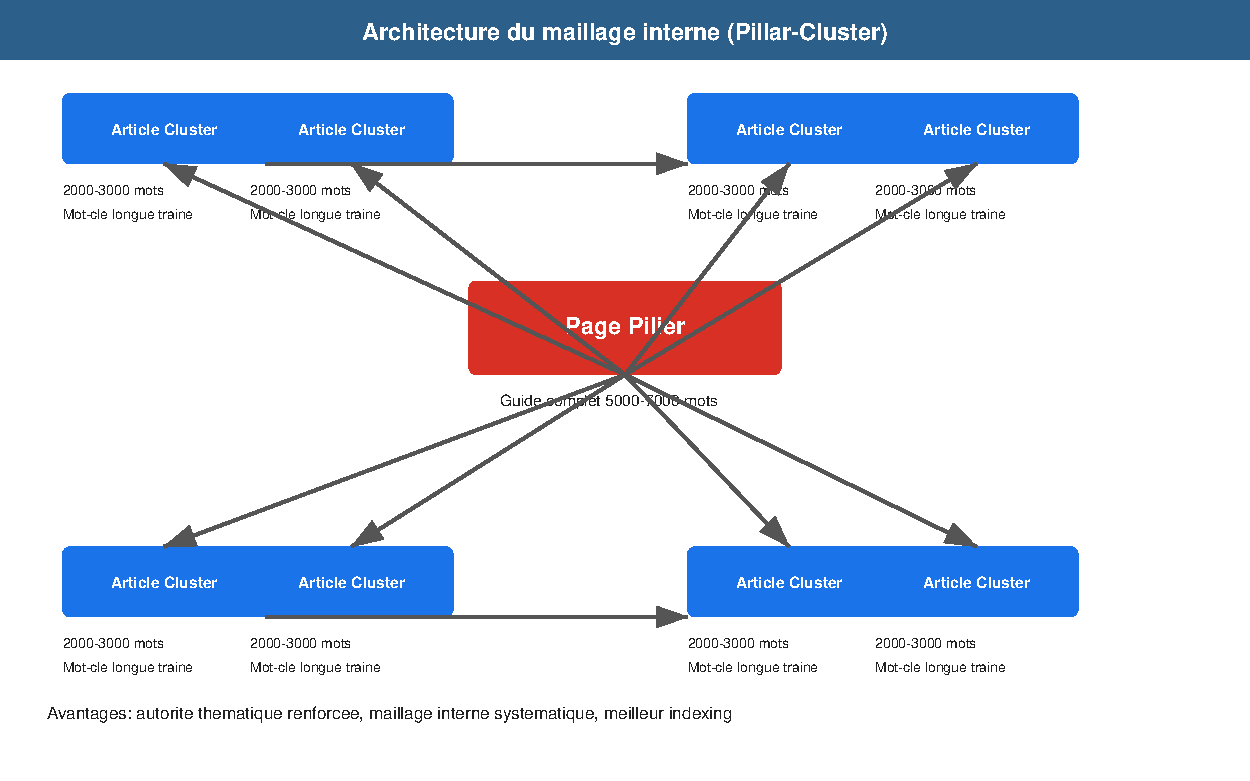
\includegraphics[width=\textwidth]{images/internal_linking.pdf}
    \caption{Architecture du maillage interne en structure pillar-cluster}
    \label{fig:internal_linking}
\end{figure}

\section{Stratégie d'architecture du maillage interne}

Le \keyword{maillage interne} est la structure des liens qui relient les pages d'un même site. Une architecture bien conçue constitue l'un des leviers SEO les plus puissants et les plus sous-estimés.

\subsection{Les objectifs fondamentaux}

Un maillage interne efficace remplit quatre objectifs essentiels :
\begin{itemize}
    \item Distribue le PageRank (autorité) entre les pages
    \item Guide le Googlebot vers les pages importantes
    \item Améliore la navigation utilisateur et les signaux comportementaux
    \item Crée des \keyword{Topical Clusters} (clusters thématiques)
\end{itemize}

\subsection{Architecture en silo}

L'architecture en \keyword{silo} organise le contenu en catégories thématiques étanches. Chaque silo regroupe des pages autour d'un sujet principal, avec des liens internes confinés au silo pour concentrer l'autorité thématique :

\begin{lstlisting}[style=htmlcode,caption={Architecture en silo pour un site e-commerce}]
Silo 1: Chaussures de Running
  |-- Page pilier: "Guide des chaussures de running"
  |     |-- Article: "Chaussures pour marathon"
  |     |-- Article: "Chaussures pour trail"
  |     |-- Article: "Chaussures pour piste"
  |     |-- Produit: "Nike Air Zoom Tempo"
  |     |-- Produit: "Hoka Clifton 9"

Silo 2: Chaussures de Ville
  |-- Page pilier: "Guide des chaussures urbaines"
  |     |-- Article: "Chaussures habillées"
  |     |-- Article: "Baskets lifestyle"
  |     |-- Produit: "Veja V-10"
  |     |-- Produit: "Adidas Stan Smith"
\end{lstlisting}

\subsection{Modèle Pilier-Cluster}

Le modèle \keyword{Pillar-Cluster} (ou Hub-and-Spoke) est le cadre le plus recommandé par Google. Une page pilier couvre un sujet de manière exhaustive, tandis que les pages clusters approfondissent des sous-sujets spécifiques. Chaque page cluster pointe vers la page pilier et vice-versa, créant un maillage bidirectionnel.

\section{La distribution du PageRank interne}

\subsection{Calcul du flux d'autorité}

Le \keyword{PageRank} se propage à travers les liens internes selon un principe de dilution : plus une page a de liens sortants, moins chaque lien transmet d'autorité. La formule simplifiée du flux est :

\[
\text{PR}_{\text{cible}} = \text{PR}_{\text{source}} \times \frac{d}{N_{\text{sortants}}}
\]

Où $d$ est le facteur d'amortissement (0,85) et $N_{\text{sortants}}$ le nombre de liens sortants de la page source.

\subsection{Principes de distribution}

\begin{mybox}{Règles de distribution du link juice}{googleyellow}
\begin{itemize}
    \item Les pages les plus importantes doivent recevoir le plus de liens internes
    \item Évitez les pages avec plus de 100 liens sortants (dilution excessive)
    \item Utilisez le \keyword{nofollow} sur les liens non essentiels (mentions légales, CGV)
    \item Les liens en début de contenu transmettent plus d'autorité que ceux en footer
    \item Un lien contextuel dans le corps du texte a plus de poids qu'un lien de navigation
\end{itemize}
\end{mybox}

\section{La diversification des ancres de lien (Anchor Text)}

La variété des \keyword{anchor texts} (textes d'ancrage) est cruciale pour un maillage naturel :

\begin{itemize}
    \item \textbf{Exact match} : Ancre identique au mot-clé ciblé (à utiliser avec modération)
    \item \textbf{Partial match} : Ancre contenant le mot-clé avec des mots additionnels
    \item \textbf{Brand} : Utilisation du nom de marque comme ancre
    \item \textbf{Générique} : « Cliquez ici », « En savoir plus », « Lire l'article »
    \item \textbf{URL nue} : L'URL complète comme ancre (ex: exemple.com/guide)
    \item \textbf{Image} : L'attribut alt de l'image sert d'ancre
\end{itemize}

\important{Une suroptimisation des ancres exact match est un signal de manipulation pour Google. Visez une répartition naturelle : 30\% brand, 30\% générique, 20\% partial match, 10\% exact match, 10\% URL.}

\section{Les types de liens internes}

\subsection{Liens contextuels}

Les \keyword{liens contextuels} situés dans le corps du contenu sont les plus puissants. Ils apportent à la fois du contexte sémantique et de l'autorité. Chaque article devrait contenir 3 à 5 liens contextuels vers des pages pertinentes.

\subsection{Liens de navigation}

\begin{itemize}
    \item \textbf{Menu principal} : Liens vers les pages piliers et catégories principales
    \item \textbf{Fil d'Ariane (Breadcrumb)} : Navigation hiérarchique avec données structurées
    \item \textbf{Footer} : Liens institutionnels (contact, mentions légales, plan du site)
    \item \textbf{Articles connexes} : Recommandations contextuelles en fin d'article
\end{itemize}

\subsection{Marquage BreadcrumbList avec Schema.org}

Le fil d'Ariane doit être balisé avec le schema \keyword{BreadcrumbList} pour apparaître dans les SERP :

\begin{lstlisting}[style=htmlcode,caption={Breadcrumb avec données structurées JSON-LD}]
<script type="application/ld+json">
{
  "@context": "https://schema.org",
  "@type": "BreadcrumbList",
  "itemListElement": [
    { "@type": "ListItem",
      "position": 1,
      "name": "Accueil",
      "item": "https://exemple.com/" },
    { "@type": "ListItem",
      "position": 2,
      "name": "Guide SEO",
      "item": "https://exemple.com/guide-seo/" },
    { "@type": "ListItem",
      "position": 3,
      "name": "Maillage interne",
      "item": "https://exemple.com/guide-seo/maillage-interne/" }
  ]
}
</script>
\end{lstlisting}

\section{Audit du maillage interne}

\subsection{Méthodologie d'audit}

Pour auditer le maillage interne d'un site :

\begin{enumerate}
    \item \textbf{Crawl complet} : Utilisez Screaming Frog SEO Spider ou Sitebulb
    \item \textbf{Analyse des pages orphelines} : Pages sans aucun lien interne entrant
    \item \textbf{Profondeur de crawl} : Nombre de clics depuis la page d'accueil
    \item \textbf{Distribution des liens} : Pages avec trop peu ou trop de liens entrants
    \item \textbf{Anchor text analysis} : Répartition des types d'ancres
    \item \textbf{Rapport de force} : Identification des pages qui reçoivent le plus de link juice
\end{enumerate}

\begin{mybox}{Outils recommandés pour l'audit}{purple}
\begin{itemize}
    \item \textbf{Screaming Frog} : Export du « Graphique des liens internes », rapport de profondeur
    \item \textbf{Sitebulb} : Visualisation de l'architecture du site, détection des orphelins
    \item \textbf{Ahrefs Site Audit} : Analyse du maillage interne avec recommandations
    \item \textbf{Google Search Console} : Rapport « Liens internes » dans la section Liens
    \item \textbf{Python + NetworkX} : Analyse avancée du graphe de liens avec calculs personnalisés
\end{itemize}
\end{mybox}

\subsection{Étude de cas : restructuration du maillage interne}

Un site éditorial de 500 articles souffrait d'un maillage plat : chaque article pointait vers 2--3 liens génériques. En restructurant l'architecture autour de 10 pages piliers avec 50 articles clusters liés bidirectionnellement :

\begin{itemize}
    \item Augmentation du trafic organique global : +45\% en 4 mois
    \item Pages piliers passées de la position 15 à la position 3 en moyenne
    \item Réduction de la profondeur de crawl moyenne : de 5 à 2,5 clics
    \item Nombre de pages indexées : +30\%
\end{itemize}

\begin{takeaways}
\begin{itemize}
    \item L'architecture en silo concentre l'autorité thématique par catégorie
    \item Le modèle pilier-cluster crée un maillage bidirectionnel puissant
    \item La diversification des ancres de lien est essentielle pour un profil naturel
    \item Les liens contextuels dans le corps du contenu transmettent le plus d'autorité
    \item Le marquage BreadcrumbList avec Schema.org améliore les SERP
    \item Un audit régulier avec Screaming Frog ou Sitebulb permet d'identifier les pages orphelines
    \item La restructuration du maillage peut générer des gains de trafic de 30 à 50\%
\end{itemize}
\end{takeaways}

\level{2}
\begin{objectives}
\begin{itemize}
    \item Comprendre les trois métriques des Core Web Vitals
    \item Savoir mesurer LCP, INP et CLS
    \item Mettre en oeuvre des optimisations ciblées
\end{itemize}
\end{objectives}

\chapter{Les Core Web Vitals}
\label{ch:corewebvitals}

\section{Présentation des Core Web Vitals}

Les \keyword{Core Web Vitals} sont un ensemble de métriques introduites par Google en 2020 pour mesurer la qualité de l'expérience utilisateur sur le web. Elles sont devenues des facteurs de classement officiels depuis juin 2021.

\begin{figure}[H]
    \centering
    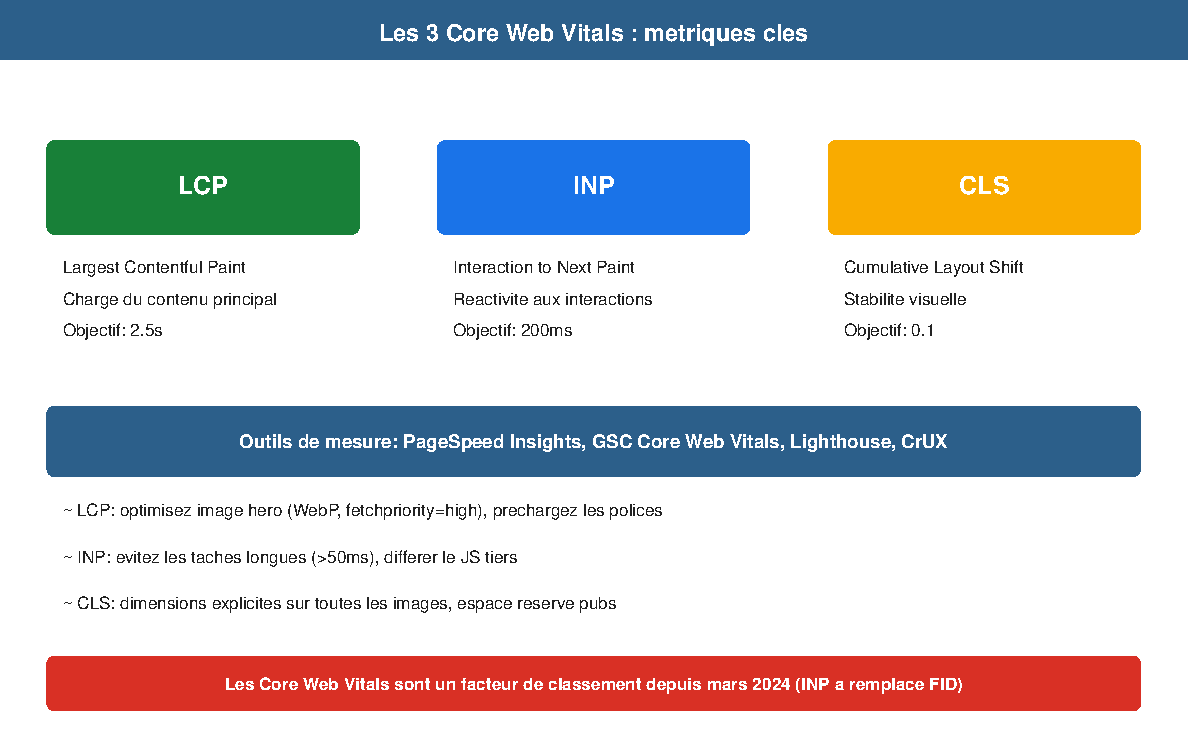
\includegraphics[width=\textwidth]{images/core_web_vitals.pdf}
    \caption{Les trois métriques des Core Web Vitals : LCP, INP et CLS avec leurs seuils d'évaluation}
    \label{fig:cvitals}
\end{figure}

\section{LCP (Largest Contentful Paint)}

Le \keyword{LCP} mesure le temps de chargement du plus grand élément visible dans la fenêtre d'affichage (image, vidéo, bloc de texte).

\begin{itemize}
    \item \textbf{Cible} : $<$ 2,5 secondes
    \item \textbf{Moyen} : 2,5 à 4 secondes
    \item \textbf{Mauvais} : $>$ 4 secondes
\end{itemize}

\subsection{Comment optimiser le LCP}

\begin{enumerate}
    \item Optimisez les images (WebP, compression, dimensions explicites)
    \item Mettez en cache les ressources statiques
    \item Réduisez le temps de réponse du serveur (TTFB)
    \item Utilisez un CDN
    \item Supprimez le JavaScript et CSS bloquant le rendu
    \item Préchargez les ressources critiques (polices, images hero)
\end{enumerate}

\section{INP (Interaction to Next Paint)}

L'\keyword{INP} remplace FID (First Input Delay) depuis mars 2024. Il mesure la réactivité globale de la page à toutes les interactions utilisateur.

\begin{itemize}
    \item \textbf{Cible} : $<$ 200 ms
    \item \textbf{Moyen} : 200 à 500 ms
    \item \textbf{Mauvais} : $>$ 500 ms
\end{itemize}

\subsection{Comment optimiser l'INP}

\begin{enumerate}
    \item Réduisez la charge JavaScript (code splitting, lazy loading)
    \item Évitez les tâches longues (main thread)
    \item Utilisez \texttt{requestIdleCallback} pour les tâches non critiques
    \item Déléguez les événements plutôt que d'attacher des listeners individuels
    \item Utilisez Web Workers pour les calculs complexes
\end{enumerate}

\section{CLS (Cumulative Layout Shift)}

Le \keyword{CLS} mesure la stabilité visuelle de la page. Un score de 0 signifie qu'aucun élément ne se déplace pendant le chargement.

\begin{itemize}
    \item \textbf{Cible} : $<$ 0,1
    \item \textbf{Moyen} : 0,1 à 0,25
    \item \textbf{Mauvais} : $>$ 0,25
\end{itemize}

\subsection{Comment optimiser le CLS}

\begin{enumerate}
    \item Définissez toujours des dimensions explicites pour les images et vidéos
    \item Réservez l'espace pour les publicités (ad slots)
    \item Évitez d'injecter du contenu au-dessus de contenu déjà affiché
    \item Utilisez \texttt{font-display: swap} pour les polices web
    \item Assurez-vous que les éléments UI (boutons, formulaires) ont des dimensions stables
\end{enumerate}

% CHAPITRE 32 (après ligne 1023, avant ch:mobilefirst)
% =============================================================================

\begin{exercise}[Audit de performance mobile]
\begin{enumerate}
    \item Analysez 3 pages d'un site avec Google PageSpeed Insights.
    \item Notez les valeurs LCP, INP, CLS pour chaque page.
    \item Identifiez les causes principales des mauvaises performances.
    \item Proposez un plan d'optimisation priorisé avec 5 actions minimum.
\end{enumerate}
\end{exercise}

\begin{takeaways}
\begin{itemize}
    \item LCP mesure la vitesse de chargement perçue
    \item INP évalue la réactivité aux interactions
    \item CLS quantifie la stabilité visuelle de la page
    \item Ces métriques sont des facteurs de classement depuis 2022
\end{itemize}
\end{takeaways}

\level{3}
\begin{objectives}
\begin{itemize}
    \item Maîtriser les stratégies CDN avancées
    \item Configurer un pipeline d'optimisation complet
    \item Implémenter HTTP/2, HTTP/3 et les resource hints
\end{itemize}
\end{objectives}

\chapter{Optimisation avancée de la performance web}
\label{ch:perfweb}

\section{Stratégies CDN (Content Delivery Network)}

Un \keyword{CDN} (Content Delivery Network) est un réseau de serveurs distribués géographiquement qui stocke en cache les ressources statiques d'un site web pour les délivrer depuis le nœud le plus proche de l'utilisateur. L'impact sur le SEO est direct : un CDN réduit considerablement le \important{TTFB} (Time To First Byte) et améliore le \keyword{LCP}.

\begin{mybox}{CDN recommandés pour le SEO}{googleblue}
\begin{itemize}
    \item \textbf{Cloudflare} : Gratuit, inclut protection DDoS, HTTP/3, Brotli
    \item \textbf{KeyCDN} : Performant, paiement à l'usage, zones de cache personnalisables
    \item \textbf{Fastly} : Cache modifiable par VCL, idéal pour les sites dynamiques
    \item \textbf{Akamai} : Solution entreprise, couverture mondiale maximale
    \item \textbf{CloudFront (AWS)} : Intégration native avec l'écosystème AWS
    \item \textbf{BunnyCDN} : Rapport qualité-prix excellent, interface simple
\end{itemize}
\end{mybox}

\subsection{Configuration avancée du CDN}

Une configuration CDN optimale pour le SEO implique :

\begin{enumerate}
    \item \textbf{Cache des ressources statiques} : CSS, JS, images, polices avec des TTL longs (30 jours minimum)
    \item \textbf{Purge sélective} : Invalider le cache uniquement pour les ressources modifiées
    \item \textbf{Origin Shield} : Un cache central qui réduit la charge sur le serveur d'origine
    \item \textbf{Edge Side Includes (ESI)} : Assemblage de pages au niveau du CDN pour du contenu dynamique
    \item \textbf{Cache du HTML} : Mise en cache des pages HTML entières avec invalidation intelligente
    \item \textbf{Règle de cache par type de contenu} : Policy différenciée pour les images, vidéos, documents
\end{enumerate}

\begin{lstlisting}[style=code,caption={Exemple de configuration des en-têtes de cache avec Cloudflare Workers}]
// Configuration avancée du cache
addEventListener('fetch', event => {
  event.respondWith(handleRequest(event.request))
})

async function handleRequest(request) {
  const response = await fetch(request)

  const cacheControl = {
    'public': true,
    'max-age': 31536000,   // 1 an pour les assets versionnes
    's-maxage': 86400,     // 1 jour au niveau du CDN
    'stale-while-revalidate': 604800,
    'stale-if-error': 86400
  }

  const headers = new Headers(response.headers)

  if (request.url.match(/\.(css|js|png|jpg|webp|svg|woff2?)$/)) {
    headers.set('Cache-Control', 'public, max-age=31536000, immutable')
  } else if (request.url.match(/\.html$/)) {
    headers.set('Cache-Control', 'public, s-maxage=3600, stale-while-revalidate=86400')
  }

  return new Response(response.body, {
    status: response.status,
    headers: headers
  })
}
\end{lstlisting}

\section{Strategies de caching}

\subsection{Cache navigateur}

Le \keyword{cache navigateur} stocke les ressources localement sur le poste du visiteur. Les en-têtes HTTP contrôlent ce comportement :

\begin{itemize}
    \item \texttt{Cache-Control: max-age=31536000} : Ressources immutables (1 an)
    \item \texttt{Cache-Control: no-cache} : Verification systématique auprès du serveur
    \item \texttt{Cache-Control: must-revalidate} : Interdiction d'utiliser une ressource périmée
    \item \texttt{ETag} : Identifiant de version pour validation conditionnelle
    \item \texttt{Last-Modified} : Date de dernière modification pour validation
\end{itemize}

\subsection{Cache serveur}

Le \keyword{cache serveur} regroupe plusieurs techniques :

\begin{itemize}
    \item \textbf{Cache d'opcode} : APCu, OPcache pour le PHP (réduction du temps d'execution de 70\%)
    \item \textbf{Cache objet} : Redis, Memcached pour les requêtes base de données
    \item \textbf{Cache de page} : Varnish Cache, NGINX FastCGI Cache
    \item \textbf{Cache de fragment} : Mise en cache partielle des blocs de page (widgets, menus)
    \item \textbf{Cache SQL} : Mise en cache des requêtes fréquentes avec Redis
\end{itemize}

\begin{lstlisting}[style=code,caption={Configuration NGINX pour le cache serveur FastCGI}]
proxy_cache_path /var/cache/nginx levels=1:2
    keys_zone=mycache:10m max_size=1g inactive=60m;

server {
    listen 80;
    server_name example.com;

    location / {
        proxy_cache mycache;
        proxy_cache_key "$scheme$request_method$host$request_uri";
        proxy_cache_valid 200 302 60m;
        proxy_cache_valid 404 1m;
        proxy_cache_use_stale error timeout updating
            http_500 http_502 http_503 http_504;

        add_header X-Cache-Status $upstream_cache_status;

        proxy_pass http://backend;
    }

    # Purge manuelle du cache (administration)
    location ~ /purge(/.*) {
        proxy_cache_purge mycache "$scheme$request_method$host$1";
    }
}
\end{lstlisting}

\subsection{Cache applicatif}

Au niveau applicatif, l'utilisation de \keyword{Redis} ou \keyword{Memcached} permet de réduire la charge sur la base de données :

\begin{itemize}
    \item Sessions utilisateur stockées en mémoire
    \item Résultats de requêtes SQL fréquentes mis en cache (TTL ajustable)
    \item Pages entières pre-rendues et servies depuis le cache
    \item Files d'attente de tâches asynchrones
    \item Compteurs et analytics en temps réel
\end{itemize}

\important{Le cache applicatif peut réduire le temps de réponse du serveur de 200--500 ms a moins de 10 ms.}

\section{Pipeline d'optimisation des images}

Les images représentent en moyenne 50\% du poids total d'une page web. Leur optimisation est cruciale.

\subsection{Formats d'image modernes}

\begin{itemize}
    \item \textbf{WebP} : Compression 30\% supérieure au JPEG, supporte partout depuis 2024
    \item \textbf{AVIF} : Compression 50\% supérieure au JPEG, base sur AV1, support croissant
    \item \textbf{JPEG XL} : Successeur de JPEG, compression sans perte et avec perte, encodage progressif
    \item \textbf{SVG} : Format vectoriel idéal pour logos, icones, illustrations
\end{itemize}

\subsection{Techniques d'optimisation}

\begin{enumerate}
    \item \textbf{Compression avec perte contrôlée} : Qualite 80--85\% pour les photos
    \item \textbf{Responsive images} : Attributs \texttt{srcset} et \texttt{sizes} pour adapter la résolution
    \item \textbf{Lazy loading natif} : \texttt{loading="lazy"} sur toutes les images hors écran
    \item \textbf{Dimensions explicites} : Toujours specifier \texttt{width} et \texttt{height} (CLS)
    \item \textbf{Prechargement des images hero} : \texttt{<link rel="preload">} pour le LCP
    \item \textbf{Image CDN} : Services comme Cloudinary, Imgix, ou imgproxy
    \item \textbf{WebP avec fallback} : Element \texttt{<picture>} avec formats multiples
\end{enumerate}

\begin{lstlisting}[style=htmlcode,caption={Balise picture avec fallback et srcset optimisé}]
<picture>
  <source
    srcset="hero-320.avif 320w,
            hero-640.avif 640w,
            hero-1280.avif 1280w,
            hero-1920.avif 1920w"
    sizes="(max-width: 320px) 280px,
           (max-width: 640px) 600px,
           (max-width: 1280px) 1200px,
           1920px"
    type="image/avif">
  <source
    srcset="hero-320.webp 320w,
            hero-640.webp 640w,
            hero-1280.webp 1280w,
            hero-1920.webp 1920w"
    sizes="(max-width: 320px) 280px,
           (max-width: 640px) 600px,
           (max-width: 1280px) 1200px,
           1920px"
    type="image/webp">
  <img src="hero-1920.jpg"
       srcset="hero-320.jpg 320w, hero-640.jpg 640w,
               hero-1280.jpg 1280w, hero-1920.jpg 1920w"
       sizes="(max-width: 320px) 280px,
              (max-width: 640px) 600px,
              (max-width: 1280px) 1200px,
              1920px"
       alt="Description de l'image"
       width="1920" height="1080"
       loading="eager"
       decoding="async"
       fetchpriority="high">
</picture>
\end{lstlisting}

\section{HTTP/2 et HTTP/3}

\subsection{HTTP/2}

Le \keyword{HTTP/2} (2015) apporte des améliorations majeures :

\begin{itemize}
    \item \textbf{Multiplexing} : Plusieurs requêtes simultanees sur une seule connexion TCP
    \item \textbf{Server Push} : Envoi proactif de ressources au client (abandonne progrèssivement)
    \item \textbf{Compression des en-têtes} (HPACK) : Reduction du volume des headers
    \item \textbf{Binaires} : Encodage binaire plus efficace que textuel
    \item \textbf{Stream prioritization} : Ordonnancement du chargement des ressources
\end{itemize}

\subsection{HTTP/3}

Le \keyword{HTTP/3} (2022) utilise \keyword{QUIC} (Quick UDP Internet Connections) au lieu de TCP :

\begin{itemize}
    \item \textbf{zéro RTT} : Connexion instantanee après la première visite
    \item \textbf{Supprèssion du Head-of-Line blocking} : Un paquet perdu ne bloque pas les autrès flux
    \item \textbf{Migration de connexion} : Changement de réseau sans reconnexion
    \item \textbf{TLS 1.3 intégré} : Chiffrement natif, pas de négociation supplementaire
    \item \textbf{Meilleure performance mobile} : Gestion optimisée des changements de réseau
\end{itemize}

\important{L'HTTP/3 peut réduire le temps de connexion initial de 1--3 allers-retours TCP a 0 RTT, soit un gain de 100 a 300 ms.}

\subsection{Migration vers HTTP/3}

\begin{enumerate}
    \item Verifiez la compatibilite de votre hebergeur / CDN
    \item Activez HTTP/3 dans la configuration du serveur ou CDN
    \item Ajoutez l'enregistrement DNS Alt-Svc
    \item Testez avec \texttt{curl --http3} ou \url{https://http3check.net}
    \item Surveillez les métriques de performance avant/après
\end{enumerate}

\section{Server Push et Resource Hints}

\subsection{Resource Hints modernes}

Le \keyword{Server Push} a ete deprecie par Chrome (2022) au profit des Resource Hints plus efficaces :

\begin{itemize}
    \item \texttt{<link rel="preload">} : Chargement prioritaire d'une ressource critique
    \item \texttt{<link rel="preconnect">} : Etablissement anticipe d'une connexion
    \item \texttt{<link rel="dns-prefetch">} : Resolution DNS anticipee
    \item \texttt{<link rel="prefetch">} : Chargement de la page suivante (navigation predite)
    \item \texttt{<link rel="prerender">} : Pre-rendu complet de la page suivante (Chrome uniquement)
    \item \texttt{<link rel="modulepreload">} : Prechargement de modules JavaScript
\end{itemize}

\begin{lstlisting}[style=htmlcode,caption={Resource Hints stratégiques pour une page optimisée}]
<!DOCTYPE html>
<html lang="fr">
<head>
  <!-- Preconnexion aux origines tierces critiques -->
  <link rel="preconnect" href="https://fonts.googleapis.com">
  <link rel="preconnect" href="https://analytics.example.com">
  <link rel="dns-prefetch" href="https://cdn.example.com">

  <!-- Prechargement des ressources LCP -->
  <link rel="preload" href="/fonts/inter-var.woff2" as="font" type="font/woff2" crossorigin>
  <link rel="preload" href="/css/critical.css" as="style">
  <link rel="preload" href="/images/hero.webp" as="image" fetchpriority="high">

  <!-- Module preload pour les apps JavaScript -->
  <link rel="modulepreload" href="/js/app.mjs">
  <link rel="modulepreload" href="/js/vendor.mjs">

  <!-- Prechargement de la page suivante (navigation predict) -->
  <link rel="prefetch" href="/produits/" as="document">
</head>
\end{lstlisting}

\section{Code Splitting et Tree Shaking}

\subsection{Code Splitting}

Le \keyword{Code Splitting} consiste a diviser le JavaScript en bundles charges à la demande :

\begin{itemize}
    \item \textbf{Entry point splitting} : Un bundle par page ou route
    \item \textbf{Vendor splitting} : Separation des bibliotheques tierces
    \item \textbf{Dynamic imports} : Importations asynchrones avec \texttt{import()}
    \item \textbf{Lazy loading de composants} : Chargement differe des composants React/Vue/Svelte
\end{itemize}

\begin{lstlisting}[style=code,caption={Code Splitting avec React.lazy et Suspense}]
import React, { lazy, Suspense } from 'react';

// Ces composants seront charges uniquement quand nécessaires
const Dashboard = lazy(() => import('./pages/Dashboard'));
const ProductList = lazy(() => import('./pages/ProductList'));
const Analytics = lazy(() => import('./pages/Analytics'));
const Settings = lazy(() => import('./pages/Settings'));

function App() {
  const [page, setPage] = useState('dashboard');

  return (
    <Suspense fallback={<LoadingSpinner />}>
      {page === 'dashboard' && <Dashboard />}
      {page === 'products' && <ProductList />}
      {page === 'analytics' && <Analytics />}
      {page === 'settings' && <Settings />}
    </Suspense>
  );
}
\end{lstlisting}

\subsection{Tree Shaking}

Le \keyword{Tree Shaking} élimine le code JavaScript mort (non utilise) lors du build :

\begin{itemize}
    \item \textbf{ES Modules} : Syntaxe \texttt{import/export} statique (requis)
    \item \textbf{Side effects} : Declaration des effets de bord dans \texttt{package.json}
    \item \textbf{Dead code elimination} : Supprèssion des fonctions et variables inutilisees
    \item \textbf{Rollup / Webpack / esbuild} : Outils supportant le tree shaking nativement
    \item \textbf{Module/nomodule pattern} : Bundle moderne pour navigateurs récents + fallback
\end{itemize}

\section{Critical CSS}

Le \keyword{Critical CSS} (ou CSS critique) consiste a extraire et inline les styles nécessaires au rendu de la partie visible de la page (above-the-fold) :

\begin{enumerate}
    \item Identifiez les styles nécessaires au rendu initial
    \item Inlinez ces styles dans le \texttt{<head>} (balise \texttt{<style>})
    \item Chargez le CSS complet de manière asynchrone
    \item Utilisez des outils comme \texttt{Critical} (Addy Osmani) ou Penthouse
\end{enumerate}

\begin{lstlisting}[style=htmlcode,caption={Critical CSS inline + chargement asynchrone}]
<head>
  <!-- Critical CSS inline (première paint) -->
  <style>
    /* Styles critiques : header, hero, navigation */
    header { display: flex; align-items: center; padding: 1rem; }
    .hero { min-height: 60vh; background: #1a1a2e; }
    nav { display: flex; gap: 2rem; }
  </style>

  <!-- Chargement asynchrone du CSS complet -->
  <link rel="preload" href="/css/styles.css" as="style"
        onload="this.onload=null;this.rel='stylesheet'">
  <noscript><link rel="stylesheet" href="/css/styles.css"></noscript>
</head>
\end{lstlisting}

\important{Le Critical CSS peut améliorer le First Contentful Paint (FCP) de 30 a 50\%.}

\section{Techniques de Lazy Loading avancées}

\subsection{Lazy loading d'images et iframes}

Le \keyword{lazy loading} natif (\texttt{loading="lazy"}) est supporte par tous les navigateurs modernes :

\begin{itemize}
    \item \texttt{loading="lazy"} : Chargement differe jusqu'a proximite du viewport
    \item \texttt{loading="eager"} : Chargement immédiat (par défaut)
    \item \texttt{decoding="async"} : Decodage asynchrone de l'image
    \item \texttt{fetchpriority="high" / "low"} : Priorite de chargement
\end{itemize}

\subsection{Lazy loading avance avec Intersection Observer}

Pour un contrôle plus fin que l'attribut natif :

\begin{lstlisting}[style=code,caption={Lazy loading avec Intersection Observer}]
const lazyImages = document.querySelectorAll('.lazy-image');

const imageObserver = new IntersectionObserver(
  (entries, observer) => {
    entries.forEach(entry => {
      if (entry.isIntersecting) {
        const img = entry.target;
        img.src = img.dataset.src;
        img.srcset = img.dataset.srcset;
        img.classList.remove('lazy');
        observer.unobserve(img);
      }
    });
  },
  {
    rootMargin: '200px 0px',
    threshold: 0.01
  }
);

lazyImages.forEach(img => imageObserver.observe(img));
\end{lstlisting}

\subsection{Lazy loading de contenu}

\begin{itemize}
    \item \textbf{Lazy loading de composants} : Chargement differe des composants React/Vue
    \item \textbf{Lazy loading de routes} : Split par route avec React Router / Vue Router
    \item \textbf{Lazy loading de commentaires} : Chargement au scroll ou au clic
    \item \textbf{Lazy loading de vidéos} : Remplacement par une vignette, chargement au clic
    \item \textbf{Infinite scroll} : Pagination asynchrone avec observer de fin de page
\end{itemize}

\section{Optimisation du TTFB (Time To First Byte)}

\subsection{Facteurs impactant le TTFB}

Le \keyword{TTFB} est le temps entre la requête HTTP et la réception du premier octet. Facteurs d'optimisation :

\begin{enumerate}
    \item \textbf{Hebergement} : Serveur géographiquement proche des utilisateurs, ressources suffisantes
    \item \textbf{Base de données} : Requêtes optimisées, index, cache Redis/Memcached
    \item \textbf{Application} : Code efficient, opcode cache, pas de boucles inutiles
    \item \textbf{Serveur web} : NGINX, LiteSpeed, OpenLiteSpeed (plus performants qu'Apache)
    \item \textbf{CDN} : Cache des pages HTML au niveau du CDN
    \item \textbf{PHP} : Version 8.x (2x plus rapide que PHP 7.x), OPcache active
\end{enumerate}

\begin{mybox}{Cibles TTFB recommandées}{googlegreen}
\begin{itemize}
    \item \textbf{Excellent} : $<$ 200 ms
    \item \textbf{Bon} : 200 -- 500 ms
    \item \textbf{A améliorer} : 500 ms -- 1 s
    \item \textbf{Critique} : $>$ 1 seconde
\end{itemize}
\end{mybox}

\section{Compression : Brotli vs Gzip}

\subsection{Brotli}

Le \keyword{Brotli} est un algorithme de compression developpe par Google, offrant un ratio de compression 20--30\% supérieur a Gzip :

\begin{itemize}
    \item \textbf{Taux de compression} : ~75--85\% de réduction (vs 60--70\% pour Gzip)
    \item \textbf{Vitesse de décompression} : Comparable a Gzip cote client
    \item \textbf{Vitesse de compression} : Plus lent que Gzip (surtout niveau 11)
    \item \textbf{Support navigateur} : 98\% des navigateurs modernes
    \item \textbf{Niveaux} : 1--11 (recommandé : niveau 5 pour l'équilibre)
\end{itemize}

\subsection{Configuration}

\begin{lstlisting}[style=code,caption={Configuration NGINX pour Brotli et Gzip}]
# Activer Brotli
brotli on;
brotli_comp_level 5;
brotli_static on;  # Sert les fichiers .br pre-comprèsses
brotli_types text/plain text/css application/json application/javascript
            application/xml text/xml application/xml+rss text/javascript
            image/svg+xml application/vnd.ms-fontobject application/x-font-ttf
            font/opentype application/wasm;

# Fallback Gzip
gzip on;
gzip_comp_level 6;
gzip_types text/plain text/css application/json application/javascript
           application/xml text/xml application/xml+rss text/javascript
           image/svg+xml;
gzip_vary on;
gzip_proxied any;
gzip_min_length 1000;
\end{lstlisting}

\important{La compression Brotli peut réduire le poids des pages HTML/CSS/JS de 20 a 30\% supplementaires par rapport a Gzip.}

\section{Optimisation base de données}

\begin{itemize}
    \item \textbf{Indexation SQL} : Index sur les colonnes utilisees dans les WHERE, JOIN, ORDER BY
    \item \textbf{Requêtes preparees} : Protection contre les injections et meilleures performances
    \item \textbf{Connection pooling} : Reutilisation des connexions base de données
    \item \textbf{Pagination cote base} : Eviter SELECT sans LIMIT, utiliser les curseurs
    \item \textbf{Requêtes N+1} : Utiliser eager loading (ex: \texttt{with()} en Laravel/Eloquent)
    \item \textbf{Read replicas} : Repartir les lectures sur des serveurs secondaires
    \item \textbf{Partitionnement} : Tables partitionnees pour les gros volumes
    \item \textbf{Nettoyage} : Purger les données obsolètes, archives des logs
\end{itemize}

\begin{lstlisting}[style=code,caption={Optimisation des requêtes N+1 avec Eloquent (Laravel)}]
// MAUVAIS : N+1 queries
$posts = Post::all();
foreach ($posts as $post) {
    echo $post->author->name; // 1 requête par post !
}

// BON : Eager loading
$posts = Post::with(['author', 'comments', 'tags'])->get();
foreach ($posts as $post) {
    echo $post->author->name; // Pas de requête supplementaire
}

// OPTIMAL : Selection des colonnes nécessaires seulement
$posts = Post::with(['author:id,name,avatar'])
    ->select(['id', 'title', 'slug', 'author_id', 'published_at'])
    ->where('published', true)
    ->orderBy('published_at', 'desc')
    ->paginate(20);
\end{lstlisting}

% =============================================================================

% ========== CHAPITRE 14 ==========
\begin{takeaways}
\begin{itemize}
    \item Le CDN réduit la latence en servant le contenu depuis le nœud le plus proche
    \item HTTP/2 et HTTP/3 améliorent significativement les performances réseau
    \item Le code splitting et le tree shaking réduisent le poids du JavaScript
\end{itemize}
\end{takeaways}

\level{2}
\begin{objectives}
\begin{itemize}
    \item Comprendre le passage au mobile-first indexing
    \item Adapter le développement aux exigences mobiles
    \item Maîtriser les techniques de rendu mobile
\end{itemize}
\end{objectives}

\chapter{Le Mobile-First Indexing}
\label{ch:mobilefirst}

\begin{figure}[H]
    \centering
    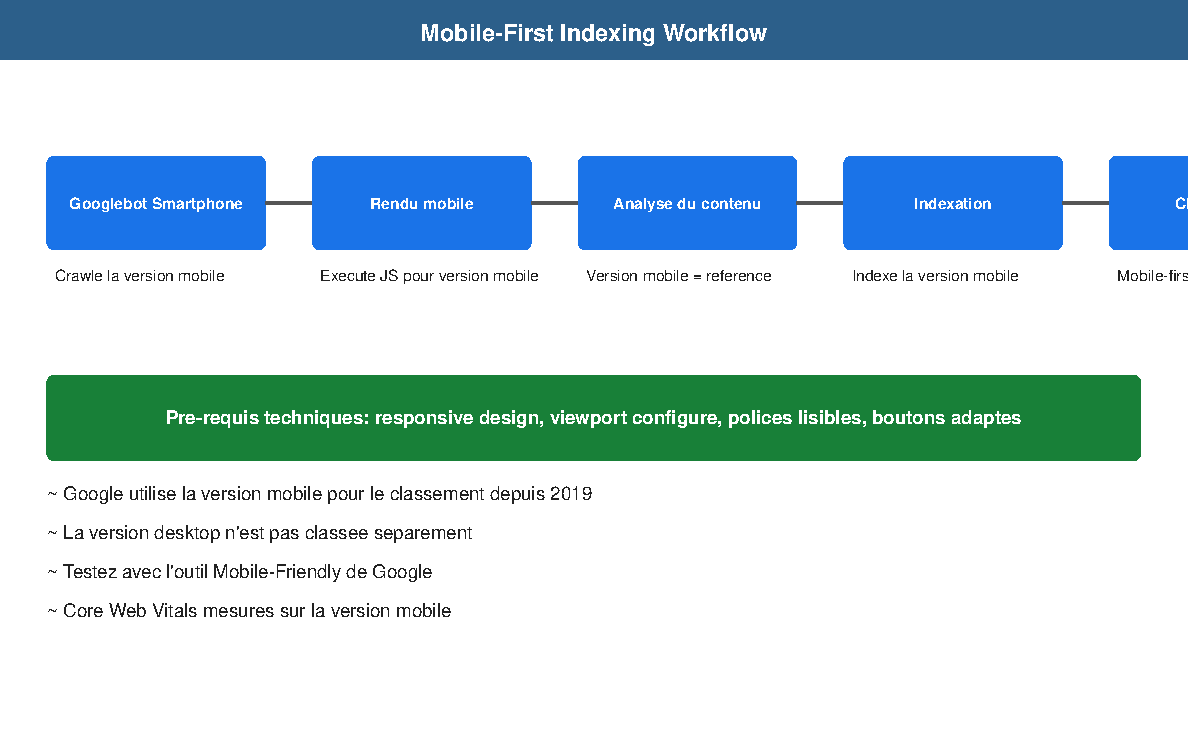
\includegraphics[width=\textwidth]{images/mobile_first.pdf}
    \caption{Workflow du Mobile-First Indexing : Google crawle et indexe d'abord la version mobile}
    \label{fig:mobile_first}
\end{figure}

\section{Le virage mobile de Google}

Depuis 2019, Google utilise \keyword{l'indexation mobile-first} (Mobile-First Indexing) comme méthode par défaut. Cela signifie que Google utilise la version mobile de votre site pour l'indexation et le classement. Un site non optimisé pour le mobile verra sa visibilité organique gravement compromise.

\subsection{Exigences techniques fondamentales}

Pour être compatible avec le mobile-first indexing, un site doit satisfaire plusieurs exigences techniques :

\begin{mybox}{Prérequis techniques pour le mobile-first indexing}{googlered}
\begin{itemize}
    \item \textbf{Même contenu} : Le contenu HTML doit être identique sur mobile et desktop
    \item \textbf{Mêmes données structurées} : Le schema markup doit être présent sur les deux versions
    \item \textbf{Mêmes meta robots} : Les directives noindex, nofollow doivent être cohérentes
    \item \textbf{Sitemap unique} : Un seul sitemap pour les deux versions
    \item \textbf{Ressources accessibles} : CSS, JavaScript et images ne doivent pas être bloqués par robots.txt
    \item \textbf{Balise viewport} : Configuration correcte obligatoire (voir section suivante)
    \item \textbf{Redirection cohérente} : Pas de redirection mobile vers une URL inaccessible sur desktop
\end{itemize}
\end{mybox}

\section{Configuration de la viewport}

La balise \keyword{viewport} est essentielle pour le rendu mobile. Une configuration incorrecte empêche le responsive design de fonctionner :

\begin{lstlisting}[style=htmlcode,caption={Configuration correcte de la balise viewport}]
<meta name="viewport" content="width=device-width, initial-scale=1.0">
\end{lstlisting}

\begin{itemize}
    \item \texttt{width=device-width} : Ajuste la largeur de la fenêtre à celle de l'appareil
    \item \texttt{initial-scale=1.0} : Niveau de zoom initial à 100\%
    \item Évitez \texttt{maximum-scale=1.0} ou \texttt{user-scalable=no} (problème d'accessibilité)
\end{itemize}

\section{Tailles des cibles tactiles et typographie mobile}

\subsection{Touch targets}

Google recommande des \keyword{zones tactiles} d'au moins 48x48 pixels avec un espacement suffisant pour éviter les erreurs de clic :

\begin{itemize}
    \item Taille minimale des boutons et liens : 48px (hauteur et largeur)
    \item Espacement entre les éléments cliquables : minimum 8px
    \item Évitez les liens trop rapprochés dans les menus mobiles
    \item Utilisez le \texttt{padding} pour agrandir les zones cliquables sans augmenter la taille visuelle
\end{itemize}

\subsection{Tailles de police pour le mobile}

La lisibilité du texte sur mobile impacte directement les signaux comportementaux :

\begin{itemize}
    \item Taille de police minimale pour le corps de texte : 16px
    \item Taille des titres (H1) : 24--32px selon le contexte
    \item Évitez les tailles de police inférieures à 14px (illisibles sur mobile)
    \item Utilisez des unités relatives (rem, em) plutôt que des pixels pour l'adaptabilité
    \item Assurez un contraste suffisant : ratio de contraste minimum de 4.5:1
\end{itemize}

\section{Comparaison des techniques de rendu mobile}

\begin{mybox}{Responsive vs Dynamic Serving vs AMP}{googleblue}
\begin{tabular}{llll}
    \toprule
    \textbf{Critère} & \textbf{Responsive} & \textbf{Dynamic Serving} & \textbf{AMP} \\
    \midrule
    URLs uniques & Oui & Oui & Oui \\
    HTML identique & Oui & Non & Non \\
    Maintenance & Simple & Complexe & Très complexe \\
    Recommandé par Google & Oui & Acceptable & Déconseillé \\
    Performance & Variable & Optimisé & Très rapide \\
    Flexibilité & Totale & Partielle & Limitée \\
    \bottomrule
\end{tabular}
\end{mybox}

\section{Tests d'utilisabilité mobile}

\subsection{Google Mobile-Friendly Test}

Le \keyword{Google Mobile-Friendly Test} est un outil gratuit qui analyse une URL et signale les problèmes d'affichage mobile. Il vérifie :

\begin{itemize}
    \item La configuration de la viewport
    \item La taille des polices (minimum 12px requis)
    \item La taille des zones tactiles
    \item Le contenu débordant horizontalement
    \item La distance entre les éléments cliquables
\end{itemize}

\subsection{Tests dans Google Search Console}

Le rapport « Utilisabilité mobile » dans Google Search Console liste les problèmes détectés sur l'ensemble du site :

\begin{enumerate}
    \item Ouvrez GSC et sélectionnez votre site
    \item Allez dans « Expérience » $\rightarrow$ « Utilisabilité mobile »
    \item Analysez les erreurs par catégorie (viewport, clic, taille police, etc.)
    \item Corrigez les erreurs et validez via l'outil d'inspection d'URL
    \item Surveillez la résolution des erreurs dans les 2 à 4 semaines
\end{enumerate}

\section{Optimisation de la vitesse mobile}

\subsection{Facteurs spécifiques au mobile}

La vitesse de chargement sur mobile est encore plus critique que sur desktop :

\begin{itemize}
    \item Le réseau mobile est 3 à 5 fois plus lent que le WiFi en moyenne
    \item Le temps de chargement acceptable sur mobile est inférieur à 3 secondes
    \item Chaque seconde de délai supplémentaire réduit les conversions de 20\%
    \item Les Core Web Vitals sont mesurés et appliqués spécifiquement sur mobile
\end{itemize}

\subsection{Techniques d'optimisation mobile}

\begin{enumerate}
    \item Utilisez des formats d'image nouvelle génération (WebP, AVIF)
    \item Implémentez le lazy loading pour les images hors écran
    \item Réduisez le poids du JavaScript (code splitting, tree shaking)
    \item Utilisez la compression Brotli pour les ressources textuelles
    \item Servez les ressources via un CDN avec des serveurs proches des utilisateurs
    \item Minifiez CSS, JavaScript et HTML
    \item Éliminez les ressources bloquant le rendu (render-blocking resources)
\end{enumerate}

\section{Données structurées spécifiques au mobile}

Certains types de schema sont particulièrement pertinents pour le mobile :

\begin{itemize}
    \item \textbf{Organization} : Coordonnées téléphoniques avec \texttt{telephone} (clic pour appeler)
    \item \textbf{LocalBusiness} : Adresse avec lien vers Google Maps (navigation intégrée)
    \item \textbf{Product} : Prix et disponibilité visibles directement dans les SERP mobiles
    \item \textbf{Event} : Date, lieu et lien d'achat de billets optimisé pour le tactile
\end{itemize}

\begin{lstlisting}[style=htmlcode,caption={Schema Organization optimisé pour le mobile}]
<script type="application/ld+json">
{
  "@context": "https://schema.org",
  "@type": "Organization",
  "name": "Mon Entreprise",
  "telephone": "+222 12 34 56 78",
  "url": "https://exemple.com",
  "contactPoint": {
    "@type": "ContactPoint",
    "telephone": "+222 12 34 56 78",
    "contactType": "customer service"
  }
}
</script>
\end{lstlisting}

\section{Étude de cas : optimisation mobile et impact sur le classement}

Un site d'actualités a entrepris une refonte mobile complète :

\begin{itemize}
    \item \textbf{Avant} : LCP à 6,2 s, non responsive, viewport non configuré, polices à 12px
    \item \textbf{Après} : Design responsive, WebP, lazy loading, viewport correct, polices à 16px
    \item \textbf{Résultats à 3 mois} :
    \begin{itemize}
        \item LCP amélioré de 6,2 s à 2,1 s (-66\%)
        \item Trafic organique mobile : +52\%
        \item Taux de rebond mobile : -18\%
        \item Positions dans le top 10 : +40\%
    \end{itemize}
\end{itemize}

\begin{mybox}{Checklist Mobile-First complète}{googlegreen}
\begin{enumerate}
    \item Design responsive validé sur tous les appareils (mobile, tablette, desktop)
    \item Balise viewport configurée correctement
    \item Polices de taille minimale 16px pour le corps de texte
    \item Zones tactiles d'au moins 48x48 pixels
    \item Core Web Vitals optimisés (LCP $<$ 2,5 s, INP $<$ 200 ms, CLS $<$ 0,1)
    \item Images au format WebP/AVIF avec lazy loading
    \item Aucune ressource bloquée par robots.txt
    \item Mêmes données structurées sur mobile et desktop
    \item Test validé avec Google Mobile-Friendly Test
    \item Aucune erreur d'utilisabilité mobile dans GSC
\end{enumerate}
\end{mybox}

\begin{takeaways}
\begin{itemize}
    \item Google utilise la version mobile du site pour l'indexation et le classement depuis 2019
    \item Le design responsive est la configuration recommandée et la plus simple à maintenir
    \item La viewport, les tailles tactiles (48px) et les polices (16px) sont des exigences techniques
    \item Les Core Web Vitals sur mobile sont mesurés séparément et appliqués au classement
    \item Un site mobile optimisé peut voir son trafic organique augmenter de 40 à 50\%
    \item Les données structurées mobiles (Organization, LocalBusiness) améliorent l'expérience utilisateur
\end{itemize}
\end{takeaways}

\level{2}
\begin{objectives}
\begin{itemize}
    \item Comprendre le rôle de Schema.org dans le SEO
    \item Savoir implémenter les types de schema essentiels
    \item Utiliser les données structurées pour les rich snippets
\end{itemize}
\end{objectives}

\chapter{Les données structurées (Schema Markup)}
\label{ch:schema}

\begin{figure}[H]
    \centering
    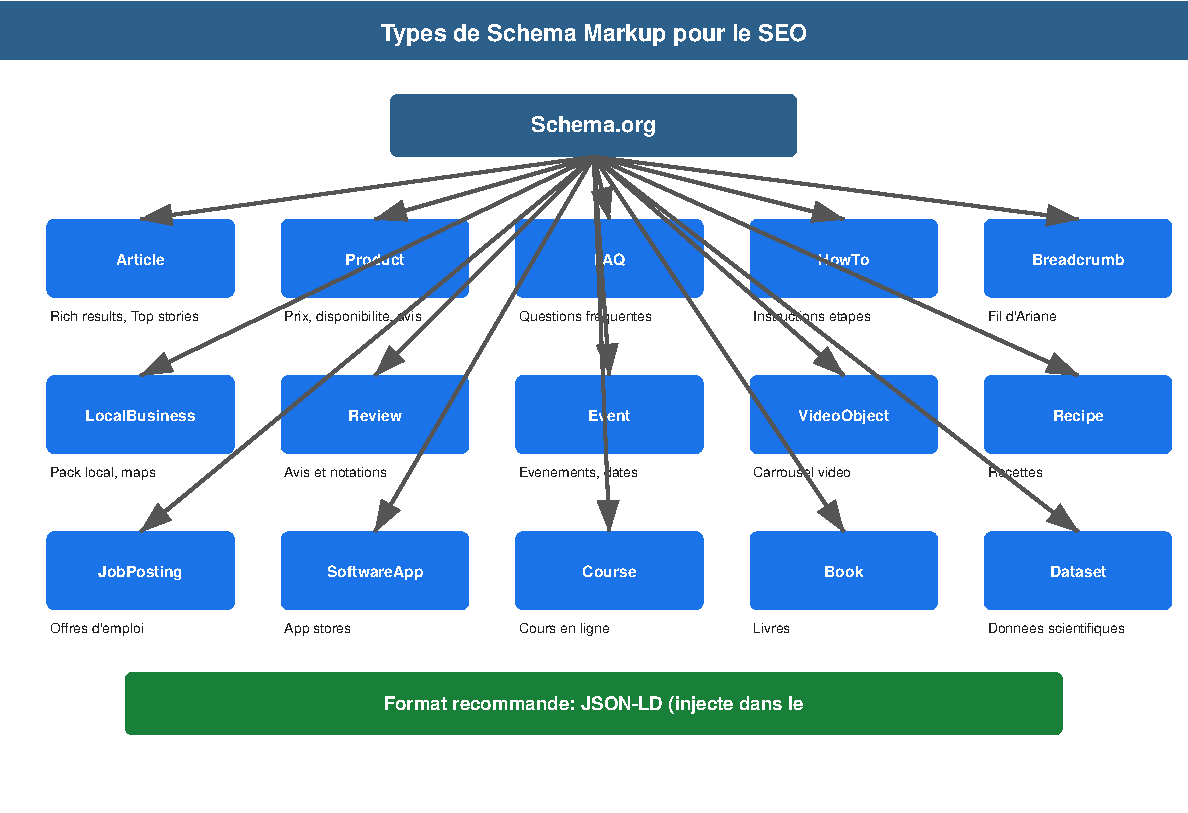
\includegraphics[width=\textwidth]{images/schema_types.pdf}
    \caption{Types de Schema Markup disponibles pour l'enrichissement des résultats dans Google}
    \label{fig:schema_types}
\end{figure}

\begin{figure}[H]
    \centering
    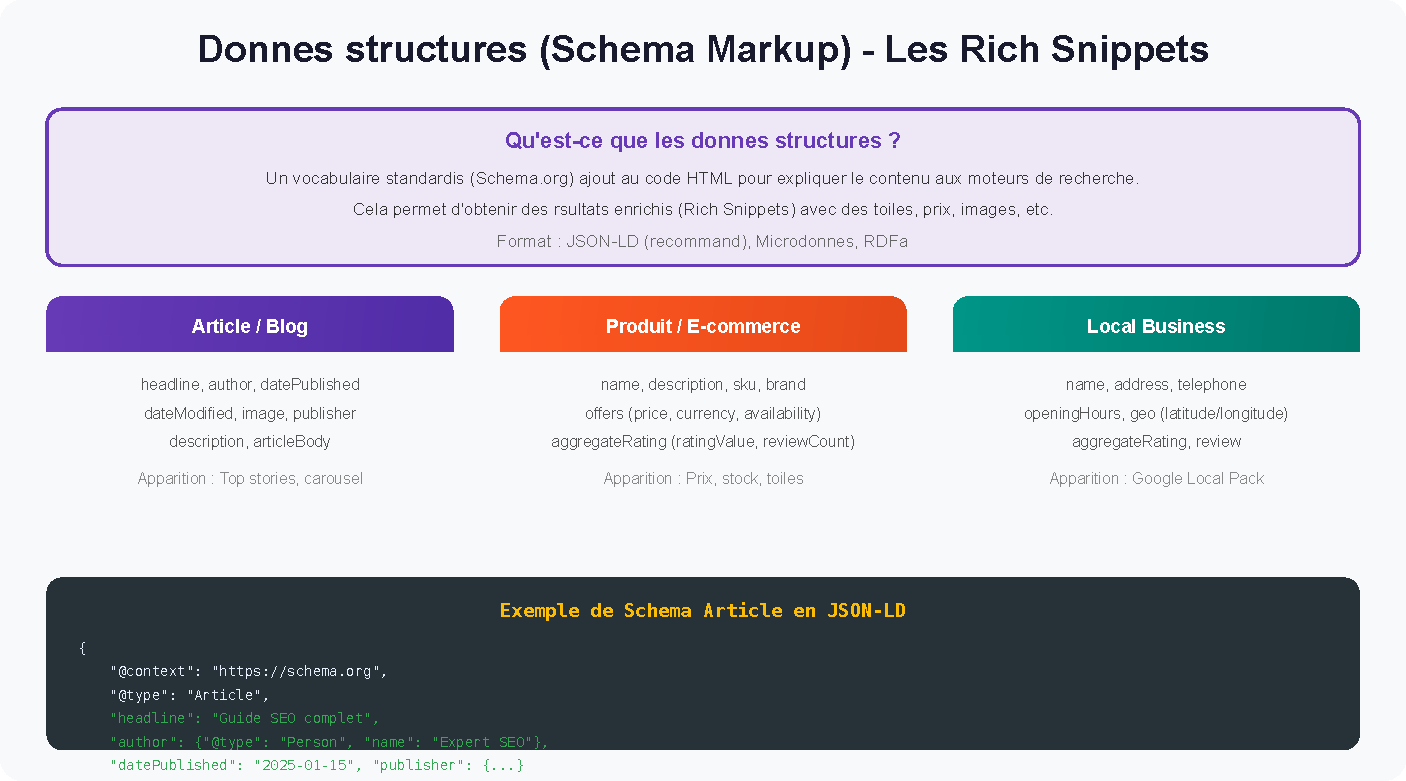
\includegraphics[width=\textwidth]{images/donnees_structurees.pdf}
    \caption{Exemple d'implémentation de données structurées avec Schema.org en JSON-LD}
    \label{fig:schema_example}
\end{figure}

\section{Présentation de Schema.org}

Les \keyword{données structurées} sont un vocabulaire standardisé (Schema.org) qui permet aux moteurs de recherche de comprendre le contenu de vos pages de manière précise et contextuelle. Lancé en 2011 par Bing, Google, Yahoo et Yandex, Schema.org est devenu le standard incontournable du web sémantique.

Les moteurs de recherche utilisent ces données pour générer des \keyword{rich snippets} (extraits enrichis) dans les SERP : étoiles d'avis, prix, dates d'événements, fils d'Ariane, etc. Ces enrichissements augmentent significativement le taux de clic (CTR).

\section{Les formats d'implémentation}

\begin{itemize}
    \item \textbf{JSON-LD} (recommandé par Google) : Script séparé dans le \texttt{<head>} ou le \texttt{<body>}
    \item \textbf{Microdata} : Attributs HTML dans les balises
    \item \textbf{RDFa} : Extension HTML pour les données liées
\end{itemize}

\subsection{JSON-LD en profondeur}

JSON-LD (JavaScript Object Notation for Linked Data) est le format privilégié par Google. Il se présente sous la forme d'un bloc \texttt{<script>} indépendant :

\begin{lstlisting}[style=htmlcode,caption={Structure JSON-LD typique}]
<script type="application/ld+json">
{
  "@context": "https://schema.org",
  "@type": "Article",
  "headline": "Titre de l'article",
  "author": {
    "@type": "Person",
    "name": "Jean Dupont"
  },
  "datePublished": "2025-06-01",
  "image": "https://example.com/image.jpg"
}
</script>
\end{lstlisting}

\subsection{Types de Schema essentiels}

\begin{mybox}{Types de Schema par catégorie}{purple}
\begin{itemize}
    \item \textbf{Article/Blog} : Article, NewsArticle, BlogPosting
    \item \textbf{Produit} : Product, Offer, AggregateRating
    \item \textbf{Entreprise locale} : LocalBusiness, Restaurant, Store
    \item \textbf{Personne} : Person, ProfilePage
    \item \textbf{Vidéo} : VideoObject
    \item \textbf{Recette} : Recipe
    \item \textbf{Événement} : Event
    \item \textbf{FAQ} : FAQPage, Question, Answer
    \item \textbf{HowTo} : HowTo, HowToStep
    \item \textbf{Breadcrumb} : BreadcrumbList
    \item \textbf{Réseau social} : SocialMediaPosting
\end{itemize}
\end{mybox}

\section{Implémentation des types majeurs}

\subsection{Article et BlogPosting}

Utilisé pour les articles de blog et les actualités :

\begin{lstlisting}[style=htmlcode,caption={Schema Article avec auteur et image}]
<script type="application/ld+json">
{
  "@context": "https://schema.org",
  "@type": "Article",
  "headline": "Guide complet du SEO en 2025",
  "description": "Tout ce qu'il faut savoir pour optimiser son site.",
  "author": {
    "@type": "Person",
    "name": "Marie Martin",
    "url": "https://example.com/auteurs/marie-martin"
  },
  "publisher": {
    "@type": "Organization",
    "name": "MonSite",
    "logo": {
      "@type": "ImageObject",
      "url": "https://example.com/logo.png"
    }
  },
  "datePublished": "2025-01-15",
  "dateModified": "2025-06-01",
  "image": "https://example.com/image-article.jpg",
  "mainEntityOfPage": {
    "@type": "WebPage",
    "@id": "https://example.com/guide-seo"
  }
}
</script>
\end{lstlisting}

\subsection{Product et Offer}

Indispensable pour le e-commerce :

\begin{lstlisting}[style=htmlcode,caption={Schema Product avec avis et prix}]
<script type="application/ld+json">
{
  "@context": "https://schema.org",
  "@type": "Product",
  "name": "Chaussures de running Pro",
  "image": "https://example.com/chaussures.jpg",
  "description": "Chaussures légères pour la course à pied.",
  "sku": "RUN-001",
  "brand": {
    "@type": "Brand",
    "name": "MarqueSport"
  },
  "offers": {
    "@type": "Offer",
    "price": "89.99",
    "priceCurrency": "EUR",
    "availability": "https://schema.org/InStock",
    "url": "https://example.com/produit/chaussures"
  },
  "aggregateRating": {
    "@type": "AggregateRating",
    "ratingValue": "4.5",
    "reviewCount": "128"
  }
}
</script>
\end{lstlisting}

\subsection{FAQPage et HowTo}

\begin{lstlisting}[style=htmlcode,caption={Schema FAQPage}]
<script type="application/ld+json">
{
  "@context": "https://schema.org",
  "@type": "FAQPage",
  "mainEntity": [{
    "@type": "Question",
    "name": "Qu'est-ce que le SEO ?",
    "acceptedAnswer": {
      "@type": "Answer",
      "text": "Le SEO (Search Engine Optimization) est l'ensemble des techniques visant à optimiser un site web pour les moteurs de recherche."
    }
  },{
    "@type": "Question",
    "name": "Combien de temps faut-il pour voir des résultats SEO ?",
    "acceptedAnswer": {
      "@type": "Answer",
      "text": "Les résultats SEO apparaissent généralement entre 3 et 6 mois après le début d'une stratégie."
    }
  }]
}
</script>
\end{lstlisting}

\subsection{BreadcrumbList et LocalBusiness}

\begin{lstlisting}[style=htmlcode,caption={Schema BreadcrumbList}]
<script type="application/ld+json">
{
  "@context": "https://schema.org",
  "@type": "BreadcrumbList",
  "itemListElement": [{
    "@type": "ListItem",
    "position": 1,
    "name": "Accueil",
    "item": "https://example.com"
  },{
    "@type": "ListItem",
    "position": 2,
    "name": "Produits",
    "item": "https://example.com/produits"
  },{
    "@type": "ListItem",
    "position": 3,
    "name": "Chaussures de running",
    "item": "https://example.com/produits/chaussures"
  }]
}
</script>
\end{lstlisting}

\section{Validation et tests}

Google fournit deux outils pour valider les données structurées :

\begin{itemize}
    \item \textbf{Rich Results Test} : Teste si vos données sont éligibles aux rich snippets Google
    \item \textbf{Schema Markup Validator} : Validation technique complète du vocabulaire Schema.org
\end{itemize}

\important{Toujours tester vos données structurées après chaque modification. Une erreur de syntaxe JSON peut rendre tout le bloc invalide.}

\subsection{Erreurs fréquentes}

\begin{mybox}{Erreurs courantes et solutions}{googlered}
\begin{itemize}
    \item \textbf{JSON invalide} : Virgule manquante, guillemets non échappés -- Utilisez un validateur JSON
    \item \textbf{Types incompatibles} : Ex. Article utilisé pour une page produit -- Utilisez le type approprié
    \item \textbf{Valeurs manquantes} : Propriétés requises non fournies -- Consultez la documentation Schema.org
    \item \textbf{URL relatives} : Les URLs doivent être absolues (https://...)
    \item \textbf{Données non visibles} : Le contenu du schema doit correspondre au contenu visible de la page
\end{itemize}
\end{mybox}

\section{Schema et E-E-A-T}

Les données structurées contribuent à renforcer les signaux d'\keyword{E-E-A-T} (Expérience, Expertise, Autorité, Confiance). L'utilisation de \texttt{author}, \texttt{organization} et \texttt{review} permet de démontrer la crédibilité du contenu. Google utilise notamment le schema \texttt{AboutPage} et \texttt{Person} pour identifier les auteurs et leurs qualifications.

\section{Cas pratique : impact sur le CTR}

Une étude menée par Search Engine Land (2024) a montré que l'ajout de données structurées \texttt{FAQPage} a amélioré le CTR de 12\% en moyenne, et l'ajout de \texttt{Recipe} schema pour un site culinaire a augmenté le trafic organique de 38\%. Les rich snippets dominent visuellement les SERP, attirant l'attention des utilisateurs.

\begin{mybox}{Bonnes pratiques}{googlegreen}
\begin{itemize}
    \item Implémentez au moins \texttt{BreadcrumbList}, \texttt{Article} et \texttt{Organization}
    \item Utilisez des générateurs automatiques pour les CMS (Yoast SEO, Rank Math)
    \item Surveillez les rapports "Améliorations" dans Google Search Console
    \item Ne surchargez pas vos pages avec des données non pertinentes
\end{itemize}
\end{mybox}

% ========== CHAPITRE 16 ==========
\begin{takeaways}
\begin{itemize}
    \item Schema.org fournit un vocabulaire standardisé pour les données structurées
    \item Les rich snippets améliorent le CTR dans les SERP
    \item JSON-LD est le format recommandé par Google
    \item Chaque type de schema a des propriétés requises spécifiques
    \item La validation technique est indispensable avant déploiement
\end{itemize}
\end{takeaways}

\level{3}
\begin{objectives}
\begin{itemize}
    \item Comprendre les défis du JavaScript pour le référencement
    \item Maîtriser les stratégies de rendu : SSR, SSG, hydratation
    \item Savoir vérifier et déboguer le rendu JavaScript
\end{itemize}
\end{objectives}

\chapter{Le JavaScript SEO}
\label{ch:jsseo}

\begin{figure}[H]
    \centering
    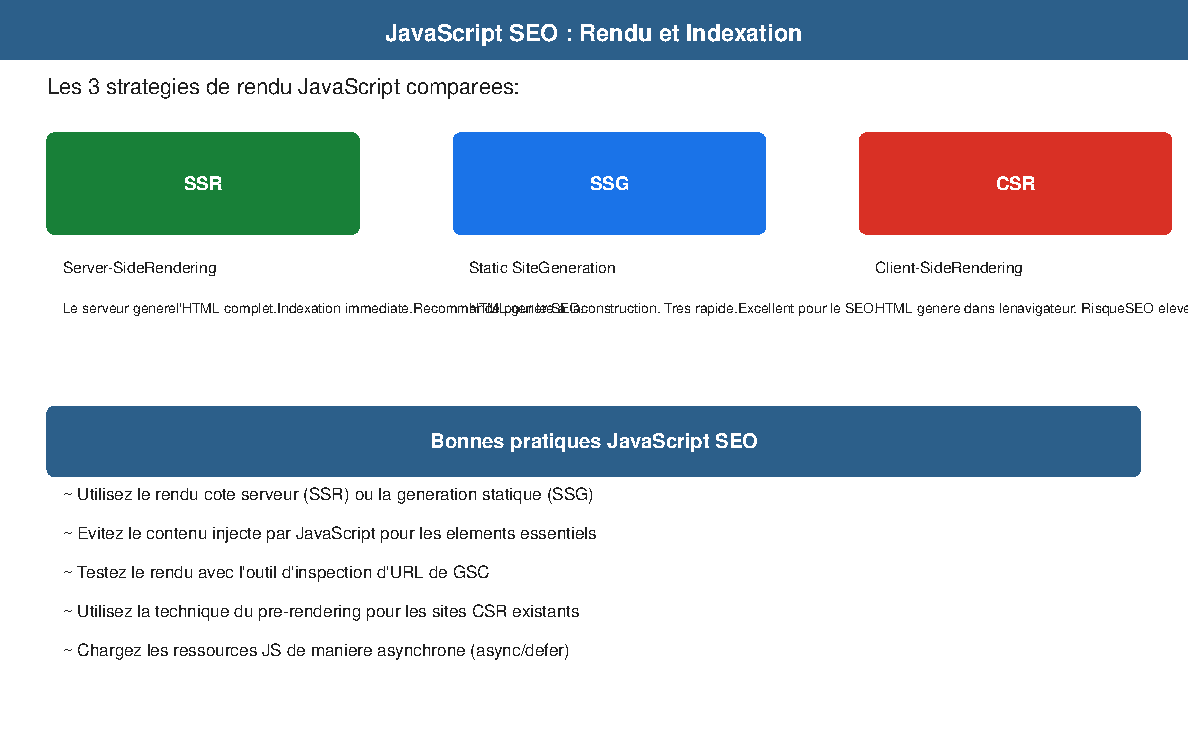
\includegraphics[width=\textwidth]{images/js_seo.pdf}
    \caption{Stratégies de rendu JavaScript : SSR, SSG et CSR comparées pour le SEO}
    \label{fig:js_seo}
\end{figure}

\section{Les défis du JavaScript pour le référencement}

Avec la popularité croissante des frameworks JavaScript (React, Next.js, Vue.js, Angular), le \keyword{JavaScript SEO} est devenu une compétence essentielle pour les développeurs web. Les moteurs de recherche doivent exécuter le JavaScript pour voir le contenu, ce qui ajoute de la complexité.

\subsection{Problèmes courants}

\begin{itemize}
    \item \important{Contenu non indexable} : Le contenu chargé par JavaScript peut ne pas être vu par Googlebot
    \item \important{Timeouts de rendu} : Googlebot a un temps limité pour render une page (environ 30 secondes sur mobile)
    \item \important{Ressources bloquées} : CSS ou JavaScript essentiels bloqués par robots.txt
    \item \important{Pages vides} : Contenu qui dépend d'API externes qui ne répondent pas
    \item \important{Gestion d'état complexe} : Les applications d'une seule page (SPA) ont des défis uniques
\end{itemize}

\subsection{Comment Google traite le JavaScript}

Googlebot passe par deux étapes pour indexer une page JavaScript :

\begin{enumerate}
    \item \textbf{Crawling initial} : Googlebot télécharge le HTML brut (généralement minimal pour les SPA)
    \item \textbf{Rendu} : Googlebot met la page dans une file d'attente pour le rendu avec Chrome
    \item \textbf{Parsing du DOM final} : Une fois le JavaScript exécuté, Googlebot indexe le contenu visible
\end{enumerate}

\section{Stratégies de rendu pour le SEO}

\subsection{Server-Side Rendering (SSR)}

Le \keyword{SSR} génère le HTML complet sur le serveur avant de l'envoyer au client :

\begin{itemize}
    \item \textbf{Avantages} : Contenu 100\% visible par Googlebot, temps de chargement réduit
    \item \textbf{Frameworks} : Next.js (React), Nuxt.js (Vue), Angular Universal
    \item \textbf{Inconvénients} : Coût serveur plus élevé, Time To First Byte (TTFB) plus long
\end{itemize}

\subsection{Static Site Generation (SSG)}

Le \keyword{SSG} génère des pages HTML statiques au moment de la construction (build) :

\begin{itemize}
    \item \textbf{Avantages} : Performance maximale, sécurité, hébergement simple (CDN)
    \item \textbf{Frameworks} : Next.js (Static Export), Gatsby, Hugo, Astro
    \item \textbf{Inconvénients} : Contenu statique, régénération nécessaire pour les mises à jour
\end{itemize}

\subsection{Hydration et Island Architecture}

L'\keyword{hydration} est le processus par lequel une application JavaScript reprend le contrôle d'un HTML rendu par le serveur. Les architectures modernes explorent :

\begin{itemize}
    \item \textbf{Island Architecture} (Astro, Fresh) : Seulement des îlots d'interactivité dans une page autrement statique
    \item \textbf{Progressive Hydration} : Hydratation par priorité des composants visibles
    \item \textbf{Partial Hydration} : Seulement les composants interactifs sont hydratés
\end{itemize}

\section{Comment vérifier le rendu JavaScript}

\begin{mybox}{Outils de diagnostic JavaScript SEO}{orange}
\begin{itemize}
    \item \textbf{Google Search Console} : Rapport "Pages" > "Indexation" > "Pages avec JavaScript"
    \item \textbf{Outils d'inspection d'URL} : Visualisez le HTML rendu par Google
    \item \textbf{Chrome DevTools} : Testez avec "Googlebot" comme user-agent personnalisé
    \item \textbf{Screaming Frog SEO Spider} : Mode JavaScript rendering
    \item \textbf{Merchant Center} : Pour les sites e-commerce
    \item "Google Web Light" ne pénalise pas le JavaScript correctement implémenté
\end{itemize}
\end{mybox}

\subsection{Test pratique du rendu JavaScript}

Pour vérifier si Google voit votre contenu JavaScript :

\begin{enumerate}
    \item Ouvrez Google Search Console
    \item Utilisez l'outil d'inspection d'URL
    \item Cliquez sur "Afficher la page crawlée"
    \item Vérifiez que le contenu principal est présent dans le HTML rendu
    \item Si le contenu est absent, vérifiez que :
    \begin{itemize}
        \item Le JavaScript n'est pas bloqué par robots.txt
        \item Les appels API sont accessibles
        \item Le site ne nécessite pas de clic pour charger le contenu
    \end{itemize}
\end{enumerate}

% CHAPITRE 33 (après ligne 1184, avant ch:semantic)
% =============================================================================
\begin{takeaways}
\begin{itemize}
    \item Le JavaScript peut bloquer l'indexation s'il n'est pas correctement géré
    \item SSR et SSG sont des solutions pour le rendu JavaScript
    \item Le test d'URL dans GSC permet de vérifier le rendu Google
\end{itemize}
\end{takeaways}

\level{3}
\begin{objectives}
\begin{itemize}
    \item Comprendre les enjeux du SEO international
    \item Maîtriser l'implémentation des balises hreflang
    \item Choisir la stratégie de domaine adaptée
\end{itemize}
\end{objectives}

\chapter{SEO International et Multilingue}
\label{ch:international}

\begin{figure}[H]
    \centering
    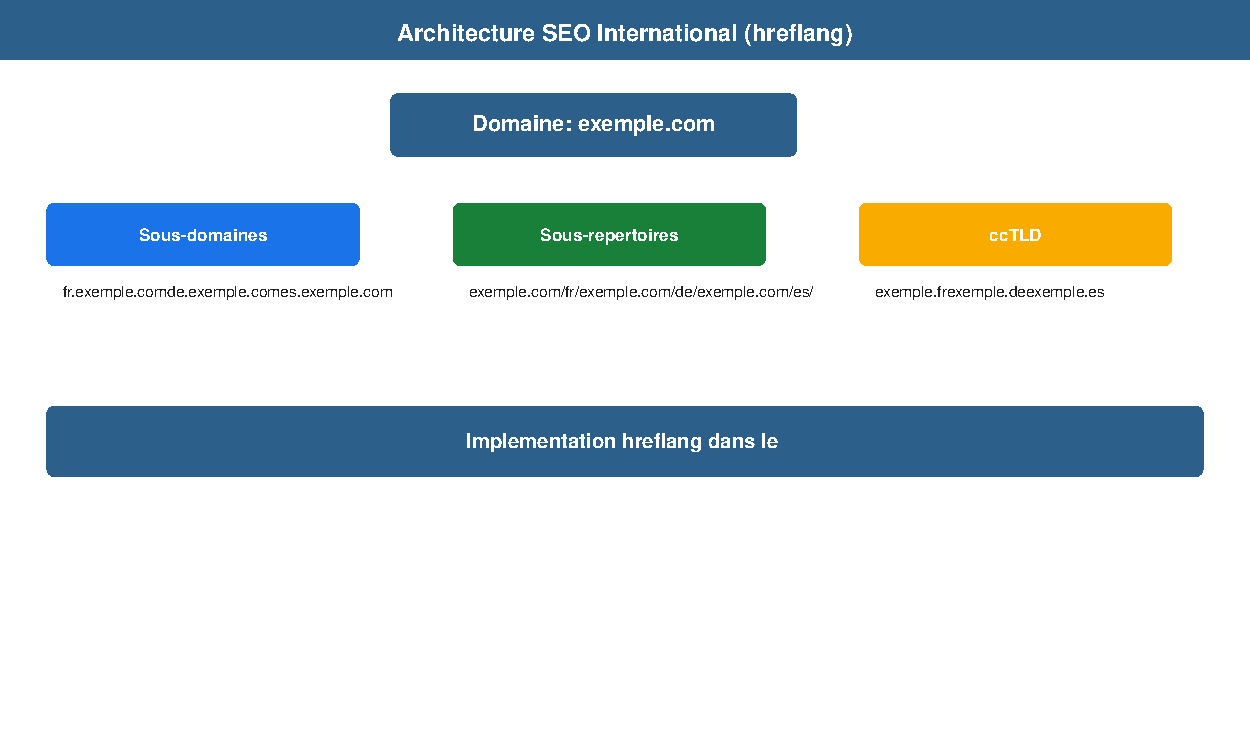
\includegraphics[width=\textwidth]{images/international_seo.pdf}
    \caption{Architectures SEO international : sous-domaines, sous-répertoires et ccTLD}
    \label{fig:international_seo}
\end{figure}

\section{Enjeux du SEO International}

Le \keyword{SEO international} consiste a optimisér un site web pour qu'il soit visible dans différents pays et langues. Contrairement au SEO local, il s'agit de déployer une stratégie cohérente à l'échelle mondiale tout en respectant les spécificités de chaque marché.

\subsection{Les défis du SEO international}

\begin{itemize}
    \item \textbf{Gestion multilingue} : Contenu duplique entre les versions linguistiques
    \item \textbf{Gestion multi-pays} : Ciblage géographique et pertinence locale
    \item \textbf{Infrastructure technique} : Architecture des URLs, DNS, hebergement
    \item \textbf{Ressources} : Traduction, adaptation culturelle, maintenance
    \item \textbf{Mesure} : Suivi des performances par pays et par langue
\end{itemize}

\section{Implementation des balises hreflang}

Les \keyword{balises hreflang} indiquent a Google quelle version linguistique ou régionale d'une page afficher dans les résultats de recherche. Une implémentation correcte est \important{cruciale} pour éviter les pénalités de contenu duplique.

\subsection{Syntaxe hreflang}

\begin{lstlisting}[style=htmlcode,caption={Implementation hreflang dans le <head>}]
<head>
  <!-- Version francaise pour la France -->
  <link rel="alternate" hreflang="fr-FR"
        href="https://example.com/fr/produits" />
  <!-- Version francaise pour la Belgique -->
  <link rel="alternate" hreflang="fr-BE"
        href="https://example.com/fr-be/produits" />
  <!-- Version francaise pour la Suisse -->
  <link rel="alternate" hreflang="fr-CH"
        href="https://example.com/fr-ch/produits" />
  <!-- Version anglaise (générique) -->
  <link rel="alternate" hreflang="en"
        href="https://example.com/en/products" />
  <!-- Version anglaise pour les US -->
  <link rel="alternate" hreflang="en-US"
        href="https://example.com/en-us/products" />
  <!-- Page par défaut (x-default) -->
  <link rel="alternate" hreflang="x-default"
        href="https://example.com/products" />
</head>
\end{lstlisting}

\subsection{Hreflang dans le sitemap}

\begin{lstlisting}[style=htmlcode,caption={Declaration hreflang dans le sitemap XML}]
<?xml version="1.0" encoding="UTF-8"?>
<urlset xmlns="http://www.sitemaps.org/schemas/sitemap/0.9"
        xmlns:xhtml="http://www.w3.org/1999/xhtml">
  <url>
    <loc>https://example.com/fr/produits</loc>
    <xhtml:link rel="alternate" hreflang="fr"
                href="https://example.com/fr/produits"/>
    <xhtml:link rel="alternate" hreflang="en"
                href="https://example.com/en/products"/>
    <xhtml:link rel="alternate" hreflang="de"
                href="https://example.com/de/produkte"/>
    <xhtml:link rel="alternate" hreflang="es"
                href="https://example.com/es/productos"/>
    <xhtml:link rel="alternate" hreflang="x-default"
                href="https://example.com/products"/>
  </url>
</urlset>
\end{lstlisting}

\subsection{Erreurs fréquentes avec hreflang}

\begin{mybox}{Erreurs hreflang a éviter}{googlered}
\begin{itemize}
    \item \textbf{Valeurs manquantes} : Pas de lien retour (reciprocite obligatoire)
    \item \textbf{Codes de langue invalides} : Utiliser ISO 639-1 (fr, en, de) et ISO 3166-1 Alpha 2 (FR, US)
    \item \textbf{Confirmation dans la page cible} : La page FR doit pointer vers EN et vice-versa
    \item \textbf{Hreflang sans canonical cohérent} : La balise canonical doit correspondre à l'alternate
    \item \textbf{Pages bloquees par robots.txt} : Les pages hreflang doivent etre crawlables
    \item \textbf{Noindex sur les pages alternatives} : Les pages avec hreflang ne doivent pas etre noindex
    \item \textbf{Hreflang incohérent avec le contenu} : Là langue declaree doit correspondre au contenu réel
\end{itemize}
\end{mybox}

\section{Strategie ccTLD vs gTLD}

\subsection{ccTLD (country code Top-Level Domain)}

Les \keyword{ccTLD} sont des domaines de premier niveau spécifiques à un pays (ex: \texttt{.fr}, \texttt{.de}, \texttt{.es}, \texttt{.co.uk}) :

\begin{itemize}
    \item \textbf{Avantages} : Signal géographique le plus fort pour Google, ancrage local
    \item \textbf{Inconvenients} : Cout eleve (multiples domaines), maintenance complexe, autorite fragmentee
    \item \textbf{Ideal pour} : Sites avec équipes locales, contenu très différencié par pays
\end{itemize}

\subsection{gTLD avec sous-répertoires}

Les \keyword{gTLD} avec sous-répertoires (ex: \texttt{example.com/fr/}, \texttt{example.com/de/}) :

\begin{itemize}
    \item \textbf{Avantages} : Autorite consolidée sur un seul domaine, maintenance simplifiée, cout réduit
    \item \textbf{Inconvenients} : Signal géographique plus faible, configuration requise dans GSC
    \item \textbf{Ideal pour} : Sites avec équipe centralisee, budget limite, SEO international debutant
\end{itemize}

\subsection{gTLD avec sous-domaines}

Les \keyword{sous-domaines} (ex: \texttt{fr.example.com}, \texttt{de.example.com}) :

\begin{itemize}
    \item \textbf{Avantages} : Organisation claire, possibilité d'hebergement separe
    \item \textbf{Inconvenients} : Google traite parfois les sous-domaines comme des sites separes
    \item \textbf{Ideal pour} : Grandes organisations avec des équipes régionales distinctes
\end{itemize}

\begin{mybox}{Recommandation stratégique}{teal}
Pour la plupart des projets, la structure \important{\texttt{example.com/lang/}} (gTLD + sous-répertoire) offre le meilleur équilibre entre autorite, maintenance et signal géographique. Utilisez les ccTLD uniquement si vous avez des équipes locales dédiées et un budget consequent.
\end{mybox}

\section{Ciblage linguistique dans Google Search Console}

Pour chaque version linguistique, il est nécessaire de configurer le ciblage dans \keyword{Google Search Console} :

\begin{enumerate}
    \item Ajoutez chaque variante (domaine, sous-domaine ou sous-répertoire) comme propriété separee
    \item Pour les gTLD : dans Parametrès $\rightarrow$ Ciblage international $\rightarrow$ Pays
    \item Pour les ccTLD : le ciblage est automatique
    \item Verifiez le rapport de performance filtre par pays
    \item Surveillez les imprèssions et clics par pays dans le rapport Performances
\end{enumerate}

\section{Geotargeting}

Le \keyword{géotargeting} permet d'indiquer a Google le pays cible d'une page :

\begin{itemize}
    \item \textbf{Google Search Console} : Parametre de ciblage international par pays
    \item \textbf{hreflang} : Pour les pages dans la meme langue mais destinees à des pays différents
    \item \textbf{Adresse locale} : Adresse et numero de téléphone local sur la page
    \item \textbf{Google Business Profile} : Profil par pays si présence physique
    \item \textbf{Hebergement local} : Serveur situe dans le pays cible
    \item \textbf{Backlinks locaux} : Liens provenant de sites du pays cible
\end{itemize}

\section{Considerations culturelles pour le SEO international}

Adapter un site à un marché ne se limite pas à la traduction :

\begin{itemize}
    \item \textbf{Mots-clés locaux} : Ne pas traduire littéralement -- rechercher les termes réellement utilises
    \item \textbf{Monnaie et prix} : Affichage dans la devise locale, format de nombre adapte
    \item \textbf{Unites de mesure} : Systeme métrique vs imperial
    \item \textbf{Format des dates} : JJ/MM/AAAA vs MM/JJ/AAAA
    \item \textbf{Couleurs et symboles} : Significations culturelles variables (rouge, vert, chiffres)
    \item \textbf{Images et visuels} : Représentation inclusive et adaptee culturellement
    \item \textbf{Reglementation} : RGPD (UE), cookie laws, mentions legales par pays
\end{itemize}

\section{Gestion du contenu duplique multilingue}

Le contenu duplique entre les versions linguistiques est un \important{défi majeur} du SEO international :

\begin{enumerate}
    \item \textbf{Contenu traduit professionnellement} : Eviter la traduction automatique pure (Google Translate)
    \item \textbf{Contenu adapte} : Aller au-délà de la traduction -- adapter les exemples, références
    \item \textbf{Localisation des URLs} : URLs descriptives dans chaque langue
    \item \textbf{Balises hreflang} : Indiquer clairement les relations entre les versions
    \item \textbf{Canonical auto-référençant} : Chaque version pointe vers elle-meme comme canonical
    \item \textbf{Eviter la traduction automatique non revue} : Google peut pénaliser le contenu de faible qualité
\end{enumerate}

\begin{lstlisting}[style=htmlcode,caption={Canonical et hreflang combines correctement}]
<head>
  <!-- Canonical auto-référençant -->
  <link rel="canonical" href="https://example.com/fr/produits" />

  <!-- Hreflang -->
  <link rel="alternate" hreflang="fr" href="https://example.com/fr/produits" />
  <link rel="alternate" hreflang="en" href="https://example.com/en/products" />
  <link rel="alternate" hreflang="de" href="https://example.com/de/produkte" />
  <link rel="alternate" hreflang="x-default" href="https://example.com/products" />

  <!-- Meta tags linguistiques -->
  <meta http-equiv="content-language" content="fr-FR">
</head>
\end{lstlisting}

\section{URL structure : sous-répertoires vs sous-domaines}

\subsection{Comparaison detaillee}

\begin{itemize}
    \item \textbf{Sous-repertoires (\texttt{/fr/}, \texttt{/en/})} :
    \begin{itemize}
        \item Autorite consolidée sur le domaine principal
        \item Maintenance plus simple
        \item Cookies partages entre les langues
        \item Configuration CDN plus simple
    \end{itemize}
    \item \textbf{Sous-domaines (\texttt{fr.}, \texttt{en.})} :
    \begin{itemize}
        \item Peuvent etre heberges sur des serveurs différents
        \item Google les traite parfois comme des sites distincts
        \item Possibilite de ciblage géographique par serveur
        \item Plus complexe a maintenir
    \end{itemize}
\end{itemize}

\section{SEO technique pour site multilingue}

\begin{enumerate}
    \item \textbf{Sitemap XML multilingue} : Un seul sitemap avec toutes les variantes où un sitemap par langue
    \item \textbf{Detection de là langue} : Redirection automatique basee sur Accept-Language (avec option de changement)
    \item \textbf{Cookies de préférence} : Memoriser le choix de langue de l'utilisateur
    \item \textbf{Pagination cohérente} : Structure de pagination parallele entre les langues
    \item \textbf{Vitesse} : CDN adapte à chaque région du monde
    \item \textbf{Mobile-first} : Test mobile par version linguistique
\end{enumerate}

\begin{lstlisting}[style=code,caption={Detection de là langue cote serveur avec PHP}]
<?php
// Detection de là langue preferee du navigateur
$langues_acceptees = $_SERVER['HTTP_ACCEPT_LANGUAGE'];
$langues_disponibles = ['fr', 'en', 'de', 'es'];

$langue = 'en'; // Langue par défaut

foreach (explode(',', $langues_acceptees) as $acceptee) {
    $code = substr($acceptee, 0, 2);
    if (in_array($code, $langues_disponibles)) {
        $langue = $code;
        break;
    }
}

// Verifier si l'utilisateur a déjà fait un choix
if (!isset($_COOKIE['lang'])) {
    setcookie('lang', $langue, time() + 365*24*3600, '/');
    header("Location: /$langue" . $_SERVER['REQUEST_URI']);
    exit;
}
?>
\end{lstlisting}

% =============================================================================

% ========== CHAPITRE 17 ==========
\begin{takeaways}
\begin{itemize}
    \item Les balises hreflang indiquent la langue et la région d'une page
    \item Le choix entre ccTLD, sous-domaine et sous-répertoire a un impact SEO
    \item L'adaptation culturelle est aussi importante que la traduction
\end{itemize}
\end{takeaways}

\level{2}
\begin{objectives}
\begin{itemize}
    \item Comprendre le passage du mot-clé à l'entité
    \item Maîtriser le Knowledge Graph et le SEO sémantique
    \item Implémenter une stratégie de SEO sémantique
\end{itemize}
\end{objectives}

\chapter{Le SEO Sémantique et Entity SEO}
\label{ch:semantic}

\begin{figure}[H]
    \centering
    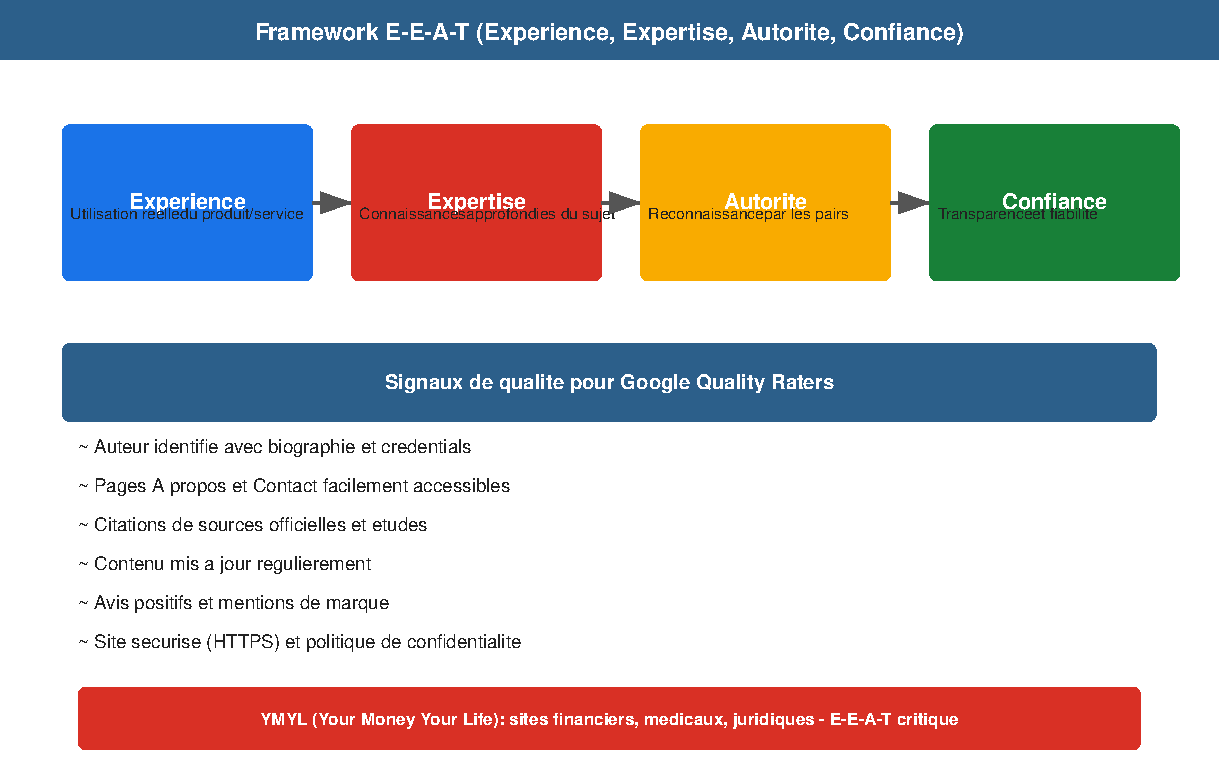
\includegraphics[width=\textwidth]{images/eeat_framework.pdf}
    \caption{Le framework E-E-A-T : Expérience, Expertise, Autorité, Confiance}
    \label{fig:eeat_framework}
\end{figure}

\section{Du mot-clé à l'entité}

Le SEO moderne a évolué d'une approche centrée sur les mots-clés à une approche centrée sur les \keyword{entités} (Entity SEO). Une entité est un concept ou un objet unique et identifiable (personne, lieu, organisation, concept). Cette évolution reflète la capacité croissante des moteurs de recherche à comprendre le sens réel du contenu, et non plus seulement à faire correspondre des chaînes de caractères.

\subsection{Qu'est-ce qu'une entité ?}

Dans le contexte du SEO, une entité se définit comme un élément distinct, unique et identifiable. Contrairement à un mot-clé qui est une simple chaîne de texte, une entité porte une signification intrinsèque. Par exemple, \texttt{Paris} n'est pas seulement un mot de cinq lettres : c'est une entité qui possède des attributs (capitale de la France, population, monuments) et des relations avec d'autres entités (la France, la Tour Eiffel, le fleuve Seine).

\subsection{Le Knowledge Graph de Google}

Google utilise un \keyword{Knowledge Graph} pour comprendre les relations entre les entités. Lancé en 2012, il contient aujourd'hui plusieurs milliards d'entités et des dizaines de milliards de relations. Par exemple, Google sait que "Paris" est une ville, qu'elle est en France, et que la Tour Eiffel s'y trouve. Cette compréhension permet à Google de fournir des résultats plus pertinents et d'enrichir les SERP avec des Knowledge Panels.

\begin{mybox}{Sources du Knowledge Graph}{googleblue}
\begin{itemize}
    \item \textbf{Wikidata} : Base de connaissances collaborative de la Wikimedia Foundation
    \item \textbf{Wikipedia} : Articles encyclopédiques structurés
    \item \textbf{CIA World Factbook} : Données géopolitiques
    \item \textbf{Schema.org} : Données structurées des sites web
    \item \textbf{Google My Business} : Informations sur les entreprises locales
\end{itemize}
\end{mybox}

\section{Le SEO Sémantique}

Le \keyword{SEO sémantique} consiste à optimiser le contenu non pas pour des mots-clés spécifiques, mais pour des concepts et des thématiques. Il s'agit de démontrer une expertise complète sur un sujet.

\begin{mybox}{Principes du SEO sémantique}{teal}
\begin{itemize}
    \item \textbf{Couverture thématique complète} : Traitez un sujet dans toutes ses dimensions
    \item \textbf{Champ sémantique} : Utilisez un vocabulaire riche et varié autour du sujet principal
    \item \textbf{Relations entre entités} : Montrez comment les concepts s'articulent entre eux
    \item \textbf{Topical Authority} : Devenez une référence sur un sujet aux yeux de Google
    \item \textbf{TF-IDF et LSI} : Termes associés naturellement présents dans un contenu expert
\end{itemize}
\end{mybox}

\subsection{Comment implémenter le SEO sémantique}

\begin{enumerate}
    \item Identifiez l'entité principale de votre contenu
    \item Listez les entités secondaires liées
    \item Utilisez les données structurées (Schema.org) pour identifier les entités
    \item Créez un contenu exhaustif qui couvre le sujet en profondeur
    \item Utilisez le maillage interne pour connecter les pages traitant d'entités connexes
    \item Analysez les "People Also Ask" et les "Related Searches" pour identifier les sous-sujets
\end{enumerate}

\section{Entity SEO : extraction et saillance}

L'extraction d'entités consiste à identifier automatiquement les entités présentes dans un texte. Google utilise le \keyword{Natural Language Processing} (NLP) pour déterminer la \keyword{sailance} (salience) de chaque entité, c'est-à-dire son importance relative dans le contexte du contenu.

Les outils d'analyse d'entités permettent d'évaluer si votre contenu couvre correctement les entités attendues pour un sujet donné :

\begin{itemize}
    \item \textbf{Google Cloud Natural Language API} : Analyse d'entités avec scores de saillance
    \item \textbf{TextRazor} : Extraction d'entités et analyse de relations sémantiques
    \item \textbf{Yahoo Content Analysis} : API d'extraction d'entités et de concepts
    \item \textbf{InLinks} : Plateforme dédiée à l'Entity SEO et aux topologies sémantiques
    \item \textbf{KMU} (Knowledge Mining Unit) : Outil d'analyse thématique avancée
\end{itemize}

\section{Topical Maps et stratégie de contenu}

La \keyword{topical map} (carte thématique) est une représentation structurée des entités et de leurs relations autour d'un sujet central. Elle sert de blueprint pour une stratégie de contenu sémantique :

\begin{lstlisting}[style=code,caption={Exemple de structure de topical map}]
Sujet central : "Marketing Digital"
  |-- Entite 1 : "SEO"
  |     |-- Relation : "composant de" Marketing Digital
  |     |-- Entites filles : Mots-cles, Backlinks, Technique
  |-- Entite 2 : "Reseaux Sociaux"
  |     |-- Relation : "composant de" Marketing Digital
  |     |-- Entites filles : Facebook, LinkedIn, Instagram
  |-- Entite 3 : "Email Marketing"
        |-- Relation : "composant de" Marketing Digital
        |-- Entites filles : Newsletters, Automatisation, Segmentation
\end{lstlisting}

\section{Wikipedia et Wikidata pour le SEO}

\keyword{Wikipedia} et \keyword{Wikidata} sont des sources majeures du Knowledge Graph de Google. Être présent dans ces bases améliore la reconnaissance de vos entités :

\begin{itemize}
    \item Créez une page Wikipedia pour votre marque (sous réserve de notoriété suffisante)
    \item Associez votre site aux entités Wikidata via le schema \texttt{sameAs}
    \item Utilisez les identifiants Wikidata dans vos données structurées
    \item Assurez-vous de la cohérence des informations entre Wikipedia, Wikidata et votre site
\end{itemize}

\begin{lstlisting}[style=htmlcode,caption={Association d'entités via sameAs}]
<script type="application/ld+json">
{
  "@context": "https://schema.org",
  "@type": "Organization",
  "name": "MonEntreprise",
  "sameAs": [
    "https://www.wikidata.org/entity/Q123456",
    "https://fr.wikipedia.org/wiki/MonEntreprise",
    "https://www.linkedin.com/company/monentreprise"
  ]
}
</script>
\end{lstlisting}

\section{Cas pratique : autorité thématique}

Un site de santé spécialisé dans la nutrition a appliqué une stratégie Entity SEO complète : cartographie de 150 entités liées à la nutrition, création de contenus ciblant chaque entité, maillage interne basé sur les relations sémantiques, et données structurées enrichies. Résultats après 8 mois : le trafic organique a augmenté de 65\%, et le site est apparu dans le Knowledge Panel pour 12 requêtes de marque liées à la nutrition.

% ============================================
% PARTIE 5 : SEO OFF-PAGE
% ============================================

\part{Le SEO Off-Page -- Autorité et Netlinking}
\label{part:offpage}

% ========== CHAPITRE 18 ==========
\begin{takeaways}
\begin{itemize}
    \item Le SEO sémantique va au-delà des mots-clés pour comprendre les entités
    \item Le Knowledge Graph de Google contient des milliards d'entités interconnectées
    \item L'optimisation sémantique améliore la pertinence thématique
    \item Les topical maps structurent la stratégie de contenu autour des entités
    \item Wikipedia et Wikidata renforcent la reconnaissance des entités
\end{itemize}
\end{takeaways}

\level{1}
\begin{objectives}
\begin{itemize}
    \item Comprendre les fondamentaux des backlinks
    \item Distinguer dofollow et nofollow
    \item Évaluer la qualité d'un profil de liens
\end{itemize}
\end{objectives}

\chapter{Le Netlinking et les Backlinks}
\label{ch:netlinking}

\begin{figure}[H]
    \centering
    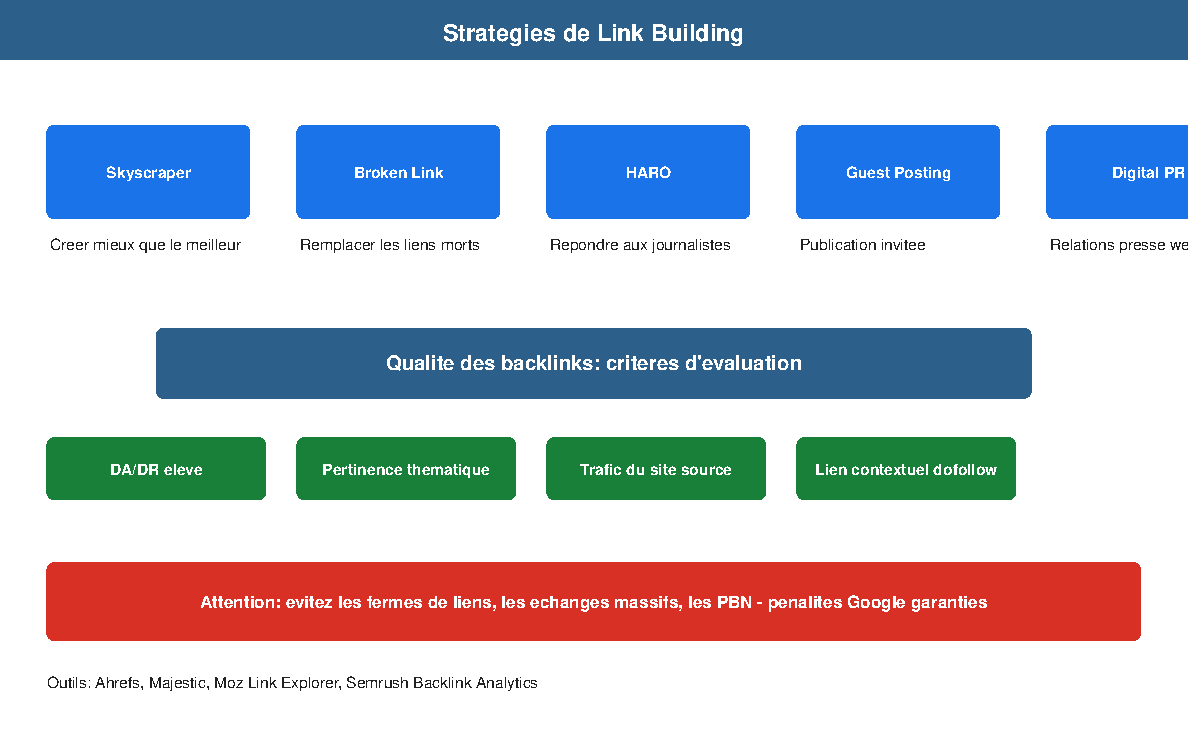
\includegraphics[width=\textwidth]{images/link_building.pdf}
    \caption{Stratégies avancées de link building et critères de qualité des backlinks}
    \label{fig:link_building}
\end{figure}

\section{Les fondamentaux des backlinks}

Les \keyword{backlinks} (liens entrants) restent l'un des facteurs de classement les plus importants de Google. Google considère chaque lien comme un vote de confiance : plus vous recevez de votes de sites de qualité, plus votre site est considéré comme une autorité. L'algorithme PageRank, inventé par Larry Page et Sergey Brin en 1998, reste à la base de cette évaluation, bien que Google utilise aujourd'hui des centaines de signaux complémentaires.

\section{Dofollow vs Nofollow vs UGC vs Sponsored}

\begin{itemize}
    \item \textbf{Dofollow} : Transmet l'autorité (PageRank). C'est le type par défaut.
    \item \textbf{Nofollow} (\texttt{rel="nofollow"}) : Ne transmet pas l'autorité. Google ignore le lien pour le PageRank.
    \item \textbf{UGC} (\texttt{rel="ugc"}) : Pour les contenus générés par les utilisateurs (commentaires, forums)
    \item \textbf{Sponsored} (\texttt{rel="sponsored"}) : Pour les liens publicitaires ou sponsorisés
\end{itemize}

Depuis 2019, Google traite les attributs \texttt{nofollow}, \texttt{ugc} et \texttt{sponsored} comme des \keyword{hints} (indices) et non plus comme des directives absolues. Google peut choisir de ne pas les prendre en compte pour le classement, mais il peut aussi décider de les ignorer. Un profil de liens naturel doit contenir un mélange équilibré de ces différents types.

\section{La qualité des backlinks}

Tous les backlinks ne se valent pas. Google évalue :

\begin{mybox}{Critères de qualité des backlinks}{googleyellow}
\begin{itemize}
    \item \textbf{Autorité du site source} : Plus le site est fort, plus le lien a de valeur
    \item \textbf{Pertinence thématique} : Un lien depuis un site du même secteur a plus de valeur
    \item \textbf{Position sur la page} : Un lien dans le contenu principal est plus fort qu'un lien dans le footer
    \item \textbf{Anchor text} : Le texte du lien doit être naturel et descriptif
    \item \textbf{Type de lien} : Dofollow $>$ Nofollow (mais un profil naturel nécessite les deux)
    \item \textbf{Nouveauté du lien} : Les liens récents ont plus de poids
    \item \textbf{Géolocalisation} : Pertinence géographique pour le SEO local
\end{itemize}
\end{mybox}

\section{Métriques d'autorité}

Plusieurs outils proposent des métriques propriétaires pour évaluer l'autorité des sites :

\begin{itemize}
    \item \textbf{Domain Authority (DA)} -- Moz : Score de 1 à 100 prédisant le classement potentiel
    \item \textbf{Domain Rating (DR)} -- Ahrefs : Qualité du profil de backlinks d'un domaine
    \item \textbf{Trust Flow (TF)} -- Majestic : Qualité des liens basée sur la confiance
    \item \textbf{Citation Flow (CF)} -- Majestic : Quantité de liens, indépendamment de la qualité
    \item \textbf{Trust Ratio} -- Majestic : Rapport Trust Flow / Citation Flow (idéalement proche de 1)
\end{itemize}

\important{Ne vous fiez pas à une seule métrique. Croisez les données de plusieurs outils pour évaluer un site correctement.}

\section{Profil de liens et link velocity}

Le \keyword{profil de liens} est l'ensemble des backlinks pointant vers un site. Google analyse sa naturalité :

\begin{itemize}
    \item \textbf{Link velocity} : La vitesse à laquelle de nouveaux liens sont acquis. Une croissance brutale est suspecte
    \item \textbf{Diversité des domaines} : Un profil sain contient des liens de nombreux domaines différents
    \item \textbf{Répartition des ancres} : Mélange naturel d'ancres exactes, partielles, de marque et génériques
    \item \textbf{Provenance géographique} : Cohérence avec la localisation du site cible
    \item \textbf{Âge du domaine} : Les liens sur un domaine récent ont moins de poids
\end{itemize}

\section{Backlinks toxiques et désaveu}

Les \keyword{backlinks toxiques} sont des liens de faible qualité ou manipulatoires qui peuvent entraîner une pénalité manuelle ou algorithmique :

\begin{mybox}{Sources de backlinks toxiques}{googlered}
\begin{itemize}
    \item Annuaires de faible qualité et fermes de liens
    \item Commentaires de blog automatisés avec lien
    \item Réseaux de sites privés (PBN)
    \item Sites adultes, casinos, pharmacie non conformes
    \item Liens payants non déclarés (sponsored)
\end{itemize}
\end{mybox}

Google propose l'outil \keyword{Disavow Links} dans Search Console pour désavouer les liens toxiques. \important{Utilisez cet outil avec prudence : un désaveu incorrect peut nuire à votre classement.}

\section{Analyse d'écart concurrentiel}

Le \keyword{competitor backlink gap analysis} consiste à identifier les sites qui linkent vers vos concurrents mais pas vers vous :

\begin{enumerate}
    \item Identifiez vos 3 à 5 concurrents principaux
    \item Extrayez leurs profils de backlinks avec Ahrefs ou Majestic
    \item Filtrez les domaines qui linkent vers au moins 2 concurrents mais pas vers vous
    \item Priorisez ces domaines pour vos campagnes de prospection
    \item Créez du contenu plus pertinent que celui de vos concurrents pour mériter ces liens
\end{enumerate}

\section{Link Reclamation et Digital PR}

Le \keyword{link reclamation} consiste à récupérer des liens perdus ou manquants :

\begin{itemize}
    \item \textbf{Mentions non liées} : Contactez les sites qui mentionnent votre marque sans lien
    \item \textbf{Liens brisés} : Proposez votre contenu comme remplacement pour des pages 404
    \item \textbf{Redirections perdues} : Mettez à jour les redirections cassées
\end{itemize}

Le \keyword{Digital PR} est l'approche moderne du netlinking : obtenir des liens grâce à des relations publiques numériques (communiqués de presse, études originales, interviews d'experts, événements en ligne).

\section{Outils de netlinking}

\begin{itemize}
    \item \textbf{Ahrefs} : Analyse de backlinks, Domain Rating, Content Explorer
    \item \textbf{Majestic} : Trust Flow, Citation Flow, historique des liens
    \item \textbf{Moz Pro} : Domain Authority, Spam Score, Link Explorer
    \item \textbf{Semrush} : Backlink Analytics, Audit de liens, Gap Analysis
    \item \textbf{Google Search Console} : Rapport "Liens" pour les données officielles
\end{itemize}

\section{Cas pratique : campagne de netlinking}

Un site e-commerce dans le secteur du sport a mis en place une stratégie combinant Digital PR et linkable assets : création d'une étude originale sur les habitudes de course à pied des Français (5000 répondants), diffusion via des communiqués de presse ciblés, et prospection manuelle auprès de 200 blogs sportifs. Résultats après 6 mois : 45 nouveaux domaines référents, augmentation de 28\% du trafic organique, et amélioration du Domain Rating de 32 à 44.

% ========== CHAPITRE 19 ==========
\begin{takeaways}
\begin{itemize}
    \item Les backlinks restent un facteur de classement majeur
    \item Un lien dofollow transmet l'autorité, un nofollow non
    \item La qualité des liens prime sur la quantité
    \item Un profil de liens naturel évite les pénalités
    \item Le Digital PR est la méthode moderne d'acquisition de liens
\end{itemize}
\end{takeaways}

\level{2}
\begin{objectives}
\begin{itemize}
    \item Maîtriser les techniques de link building modernes
    \item Comprendre le Digital PR et les linkable assets
    \item Mettre en oeuvre le broken link building
\end{itemize}
\end{objectives}

\chapter{Les stratégies avancées de Link Building}
\label{ch:linkbuilding}

\begin{figure}[H]
    \centering
    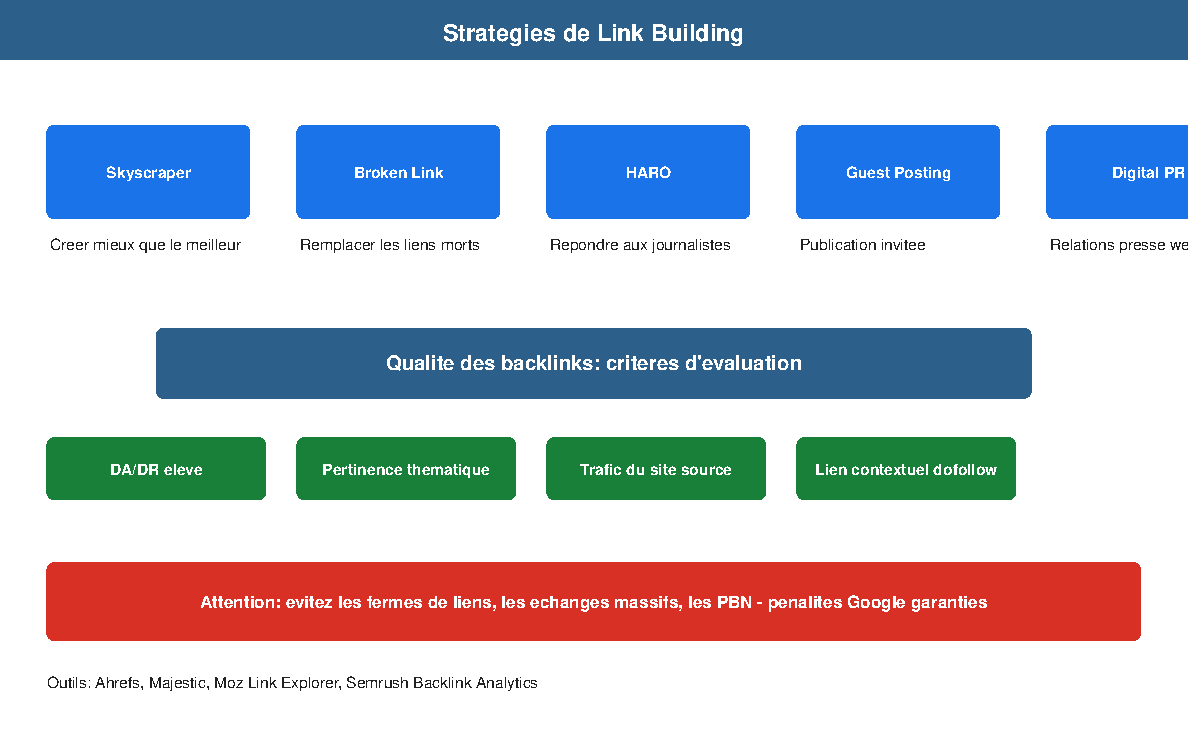
\includegraphics[width=\textwidth]{images/link_building.pdf}
    \caption{Méthodes avancées d'acquisition de backlinks et grille d'évaluation de la qualité}
    \label{fig:linkbuilding_diagram}
\end{figure}

\section{Du link building classique au Digital PR}

Le link building traditionnel (échanges de liens, annuaires, commentaires de blog) a largement perdu de son efficacité, et son usage abusif peut même déclencher des \keyword{pénalités manuelles} de Google via l'outil \textit{Disavow Links}. Les stratégies modernes se concentrent sur le \keyword{Digital PR} et la création de valeur réelle.

\subsection{Linkable Assets (Contenu magnétique)}

Créez des ressources qui attirent naturellement des liens sans démarchage :

\begin{itemize}
    \item \textbf{Études originales} : Données uniques issues de recherches ou d'enquêtes exclusives
    \item \textbf{Enquêtes et statistiques} : Analyse de données originales avec méthodologie transparente
    \item \textbf{Outils gratuits} : Calculateurs, générateurs, analyseurs (ex : calculateur de temps de chargement)
    \item \textbf{Infographies} : Visualisation de données complexes, facilement partageable
    \item \textbf{Guides exhaustifs} : Ressources de référence complètes sur un sujet (génèrent des liens \textit{reference})
    \item \textbf{Benchmarks} : Comparaisons sectorielles avec données chiffrées exclusives
\end{itemize}

\subsection{Guest Blogging et Guestographics}

Le \keyword{guest blogging} (publication invitée) reste efficace si c'est fait correctement. Une variante avancée est la \keyword{guestographics} : vous créez une infographie originale et proposez à des sites de la publier avec un lien retour.

\begin{itemize}
    \item Ciblez des sites pertinents avec une vraie audience et un trafic vérifiable
    \item Apportez une valeur réelle — ne produisez jamais de contenu médiocre
    \item Évitez les sites qui acceptent tous les articles sans sélection (fermes de contenu)
    \item Le link building est un sous-produit de la création de valeur, pas l'objectif principal
\end{itemize}

\subsection{Broken Link Building}

Cette technique gagnant-gagnant consiste à :

\begin{enumerate}
    \item Identifier des pages pertinentes avec des liens brisés (erreur 404)
    \item Créer (ou utiliser) un contenu comparable ou meilleur sur votre site
    \item Contacter le webmaster pour signaler le lien brisé
    \item Proposer votre contenu comme remplacement naturel
\end{enumerate}

\textbf{Outils de prospection} : Ahrefs Broken Link Checker, Check My Links (extension Chrome), Dead Link Checker, Screaming Frog (mode \textit{Check Links}).

\subsection{Skyscraper Technique}

Popularisée par Brian Dean (Backlinko), la \keyword{Skyscraper Technique} repose sur trois étapes : trouver un contenu populaire dans votre niche qui a déjà obtenu des backlinks, créer un contenu \textbf{significativement meilleur} (plus long, plus à jour, mieux illustré, mieux structuré), puis contacter les sites qui avaient lié le contenu original pour leur proposer votre version améliorée.

\subsection{HARO et Digital PR}

\keyword{HARO} (Help A Reporter Out) et ses équivalents français (Professionnels du PR, PressRoom) permettent aux journalistes de solliciter des experts. En répondant aux requêtes pertinentes, vous obtenez des citations avec backlinks depuis des médias reconnus, ce qui améliore directement l'autorité thématique et l'E-E-A-T.

\subsection{Unlinked Mentions et Resource Page Link Building}

Les \keyword{unlinked mentions} sont des citations de votre marque ou site sans lien hypertexte. Utilisez des outils comme Mention, Brand24 ou Google Alerts pour les détecter, puis contactez les webmasters pour demander l'ajout du lien manquant. Le \keyword{resource page link building} consiste à identifier des pages listant des ressources utiles dans votre secteur, puis à proposer d'y ajouter votre contenu s'il apporte une valeur complémentaire.

\section{Recherche de prospects et outils}

La prospection de liens nécessite des outils spécialisés :

\begin{itemize}
    \item \textbf{Ahrefs} : Site Explorer pour analyser les backlinks des concurrents, Content Explorer pour trouver des opportunités
    \item \textbf{SEMrush} : Backlink Gap Analysis pour identifier les sites qui lient vers vos concurrents mais pas vers vous
    \item \textbf{Majestic} : Trust Flow et Citation Flow pour évaluer la qualité des domaines
    \item \textbf{BuzzStream} : Gestion des campagnes d'outreach et suivi des relations
    \item \textbf{Pitchbox} : Automatisation des campagnes de link building à grande échelle
\end{itemize}

\section{Outreach : modèles et stratégies}

Un email d'outreach efficace suit une structure précise : personnalisation (mentionnez un article spécifique du site cible), valeur (expliquez pourquoi votre contenu est utile à \textit{leurs} lecteurs), proposition claire (ce que vous demandez : un lien, une citation, un partage), et facilitation (lien déjà rédigé, extrait de code prêt). \important{Évitez les emails génériques} : un taux de réponse de 5~10~\% est considéré comme bon dans le secteur.

\subsection{Link Building à grande échelle}

Pour les sites établis, le link building à grande échelle repose sur l'automatisation de la prospection (scraping de mots-clés, identification des pages ressources), la création systématique de contenu magnétique (études de données, enquêtes annuelles), et le \keyword{link reclamation} : détection systématique des backlinks perdus (via Ahrefs ou Majestic) et demande de rétablissement.

\section{Éviter les pénalités Google}

Google pénalise sévèrement les pratiques manipulatrices : achat de liens, Private Blog Networks (PBNs), échanges de liens excessifs, liens dans les pieds de page, commentaires de blog automatisés. Utilisez l'outil \keyword{Disavow Links} de Google uniquement si vous avez reçu une \textbf{pénalité manuelle}. Pour les pénalités algorithmiques (Penguin), la solution est de supprimer ou désavouer les liens toxiques et d'attendre le prochain rafraîchissement de l'algorithme.

\section{Mesure du ROI du Link Building}

Les métriques clés à suivre : nombre de \keyword{referring domains} uniques, \keyword{Domain Rating} (DR) / \keyword{Authority Score} moyen des nouveaux backlinks, trafic de référence généré par les liens, positions des pages ciblées avant/après acquisition de liens, et coût par backlink acquis. Un bon ratio est de 50~200~€ par backlink de qualité, selon le secteur et l'autorité du domaine source.

\begin{mybox}{Nouvelles approches du netlinking}{googlegreen}
\begin{itemize}
    \item \textbf{Digital PR} : Relations presse numériques pour obtenir des mentions dans les médias
    \item \textbf{Topical Authority} : Devenir une référence reconnue dans un domaine spécifique
    \item \textbf{Entity SEO} : Être associé à des entités reconnues par Google
    \item \textbf{Brand Building} : Construire une marque forte qui attire naturellement des liens
    \item \textbf{Content Syndication} : Distribution de contenu sur des plateformes autorisées (Medium, LinkedIn)
    \item \textbf{Data-driven PR} : Créer des études de données qui sont reprises par les médias
\end{itemize}
\end{mybox}

\section{Étude de cas : campagne de link building dans le secteur finance}

Une startup de comparateur d'assurances souhaitait améliorer son autorité thématique. La stratégie a combiné : une étude originale sur les économies réalisées par les consommateurs changeant d'assurance (linkable asset), une campagne HARO ciblant les journalistes finance, du broken link building sur des sites de comparaison économique, et la création de 10 articles invités sur des blogs finance reconnus. Résultats après 6 mois : 47 nouveaux referring domains, augmentation du Domain Rating de 32 à 51, progression du trafic organique de +215~\%.

% ========== CHAPITRE 20 ==========
\begin{takeaways}
\begin{itemize}
    \item Le Digital PR remplace le link building traditionnel
    \item Les linkable assets attirent naturellement des backlinks
    \item Le broken link building et la skyscraper technique sont des méthodes éprouvées
    \item La prospection d'outreach personnalisée est essentielle au succès
    \item Évitez les pratiques pénalisables et mesurez le ROI via les referring domains
\end{itemize}
\end{takeaways}

\level{2}
\begin{objectives}
\begin{itemize}
    \item Comprendre les quatre composantes d'E-E-A-T
    \item Identifier les enjeux YMYL
    \item Mettre en oeuvre une stratégie d'amélioration d'E-E-A-T
\end{itemize}
\end{objectives}

\chapter{E-E-A-T : Expérience, Expertise, Autorité, Confiance}
\label{ch:eeat}

\begin{figure}[H]
    \centering
    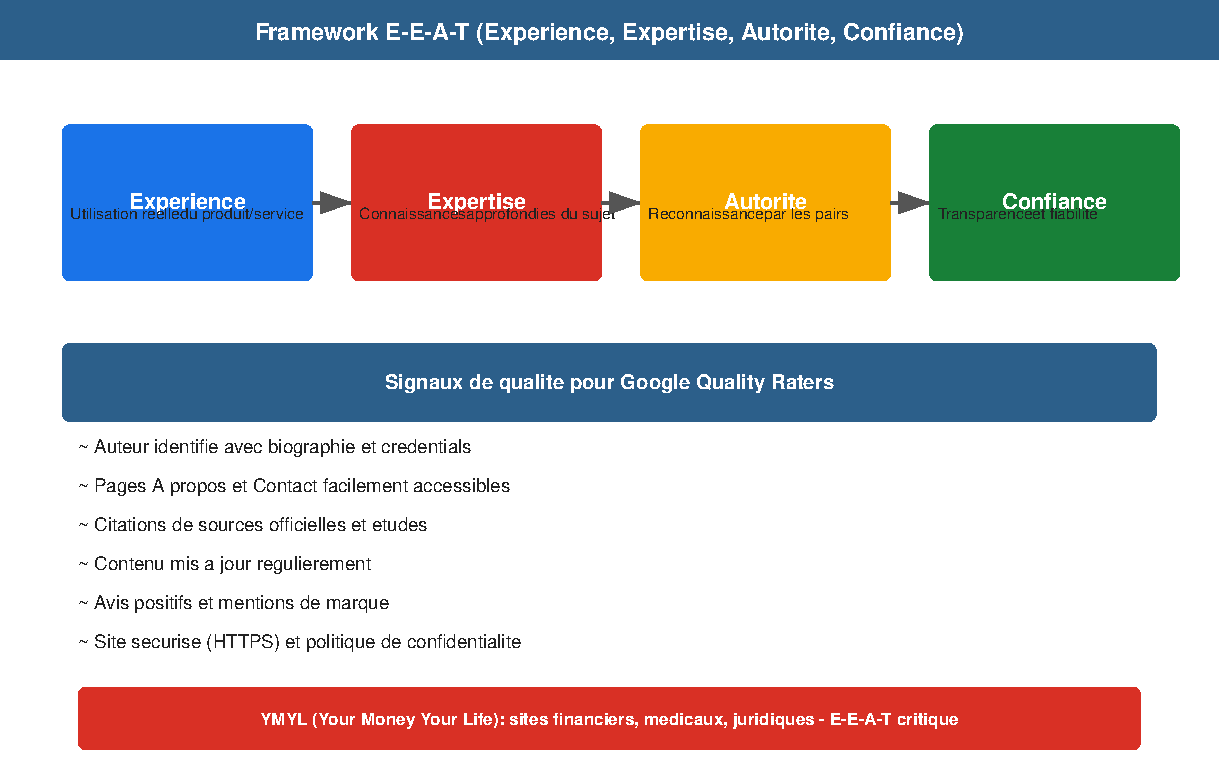
\includegraphics[width=\textwidth]{images/eeat_framework.pdf}
    \caption{Les quatre piliers du framework E-E-A-T et leurs signaux de qualité}
    \label{fig:eeat_diagram}
\end{figure}

\section{Présentation d'E-E-A-T}

Le concept d'\keyword{E-E-A-T} (Experience, Expertise, Authoritativeness, Trustworthiness) a été introduit par Google dans ses \textit{Search Quality Rater Guidelines} publiées à l'origine en 2013. Initialement connu sous le sigle \keyword{E-A-T}, Google y a ajouté un second \textbf{E} (Experience) en décembre 2022 pour insister sur l'importance de l'expérience directe. Il s'agit d'un cadre d'évaluation que Google utilise via ses \keyword{quality raters} (évaluateurs humains) pour juger la qualité du contenu. Bien que le résultat des quality raters n'impacte pas directement le classement, leurs évaluations servent à \textbf{entraîner les algorithmes} de Google.

\subsection{Les 4 composantes en détail}

\begin{description}
    \item[Experience (Expérience)] : L'auteur a-t-il une expérience directe et personnelle du sujet ? Un article sur la randonnée a plus de valeur s'il est écrit par quelqu'un qui a parcouru le GR20. Une critique de produit est plus crédible si l'auteur a réellement testé le produit. L'expérience personnelle est particulièrement valorisée pour les sujets où le vécu compte : voyages, soins de santé, produits de consommation.
    \item[Expertise (Expertise)] : L'auteur possède-t-il les qualifications nécessaires ? Formation académique, certifications professionnelles, publications académiques, reconnaissance par les pairs. Pour un article médical, un médecin diplômé a une expertise supérieure à celle d'un rédacteur web généraliste.
    \item[Authoritativeness (Autorité)] : Le site ou l'auteur est-il reconnu comme une source de référence ? Nombre et qualité des backlinks, mentions par des sources reconnues, citations dans la presse et les publications académiques, recommandations par des experts du domaine.
    \item[Trustworthiness (Confiance)] : Le site est-il digne de confiance ? Sécurité HTTPS, transparence sur l'identité de l'éditeur, mentions légales complètes, politique de confidentialité claire, absence d'erreurs factuelles, processus de correction transparent.
\end{description}

\section{Connexion avec les Google Quality Rater Guidelines}

Les \keyword{Search Quality Rater Guidelines} (QRG) sont un document de plus de 170 pages utilisé par les évaluateurs humains de Google pour juger la qualité des résultats de recherche. Les évaluateurs notent les pages selon une échelle allant de \textit{Lowest} à \textit{Highest}. Une page avec un E-E-A-T faible (contenu inexact, auteur non qualifié, site non sécurisé) reçoit une note \textit{Lowest}, tandis qu'une page avec un E-E-A-T fort obtient \textit{High} ou \textit{Highest}. Les algorithmes de Google sont ensuite ajustés pour mieux correspondre aux évaluations humaines.

\section{E-E-A-T et YMYL}

Le \keyword{YMYL} (Your Money or Your Life) désigne les pages qui peuvent impacter la santé financière, la santé physique, la sécurité ou le bien-être des utilisateurs. Ces pages sont soumises à des critères E-E-A-T beaucoup plus stricts car les conséquences d'une information erronée peuvent être graves. Google exige un E-E-A-T de niveau \textbf{très élevé} pour tout contenu YMYL.

\begin{mybox}{Catégories YMYL}{googlered}
\begin{itemize}
    \item \textbf{Santé et médecine} : Conseils médicaux, informations sur les médicaments, diagnostics
    \item \textbf{Finance} : Conseils financiers, investissement, assurance, crédit
    \item \textbf{Droit} : Conseils juridiques, documents légaux, procédures judiciaires
    \item \textbf{Sécurité} : Sécurité des produits, sécurité en ligne, sécurité des enfants
    \item \textbf{Actualités} : Information d'importance publique, politique, catastrophes
    \item \textbf{Éducation} : Formation, certification, admission universitaire
    \item \textbf{Bien-être} : Santé mentale, nutrition, développement personnel
\end{itemize}
\end{mybox}

\section{Comment l'algorithme détecte l'E-E-A-T}

Google n'utilise pas l'E-E-A-T comme un facteur de classement direct mesurable. À la place, ses algorithmes évaluent des \keyword{signaux proxy} : la crédibilité des auteurs via les données structurées \texttt{author} et \texttt{Person}, la fraîcheur et l'exactitude factuelle du contenu, la réputation du site mesurée par les backlinks et les mentions, la transparence via les pages \texttt{About}, \texttt{Contact} et les mentions légales, l'engagement utilisateur (taux de rebond, temps passé sur la page, taux de clic), et la cohérence thématique (topical authority) mesurée par la couverture complète d'un sujet. L'algorithme \textit{Medic Core Update} de 2018 a été le premier à montrer clairement que Google pouvait pénaliser des sites entiers pour un E-E-A-T insuffisant, en particulier dans les secteurs YMYL. Depuis, chaque Core Update a renforcé le poids de ces signaux dans l'évaluation globale de la qualité.

\section{Stratégie pratique pour construire les signaux E-E-A-T}

\subsection{Au niveau de la page}
\begin{itemize}
    \item Ajoutez une \keyword{byline d'auteur} avec nom, photo, biographie et lien vers une page de profil détaillée
    \item Utilisez les données structurées \texttt{author} et \texttt{Person} (Schema.org) pour lier chaque article à son auteur
    \item Citez systématiquement vos sources avec des liens vers des études, données officielles ou publications reconnues
    \item Mentionnez la date de publication et la date de dernière mise à jour
\end{itemize}

\subsection{Au niveau du site}
\begin{itemize}
    \item Créez une page \keyword{About} complète : mission de l'entreprise, équipe, méthodologie éditoriale, politique de correction
    \item Créez une page \keyword{Contact} avec adresse physique, email, téléphone, formulaire de contact
    \item Rédigez des mentions légales et une politique de confidentialité conformes au RGPD avec DPO identifié
    \item Passez en HTTPS avec un certificat SSL valide et configurez les redirections HTTP vers HTTPS
    \item Affichez les certifications, affiliations professionnelles et récompenses de manière visible
    \item Obtenez des avis vérifiés sur Google Reviews, Trustpilot, Avis Vérifiés
    \item Ajoutez une page \keyword{Équipe} avec les profils détaillés de chaque contributeur
\end{itemize}

\subsection{Au niveau de la marque}
\begin{itemize}
    \item Développez une présence dans les médias reconnus (Digital PR, relations presse, interviews)
    \item Participez à des conférences et événements professionnels en tant qu'intervenant
    \item Publiez dans des revues ou sur des plateformes reconnues (The Conversation, Medium, LinkedIn Pulse)
    \item Obtenez des backlinks depuis des sites éducatifs (.edu) ou gouvernementaux (.gouv.fr)
    \item Faites certifier votre entreprise par des organismes reconnus (ISO, labels professionnels)
    \item Encouragez les citations de votre contenu par des experts via des campagnes de Digital PR ciblées
\end{itemize}

\section{Outils pour mesurer et améliorer l'E-E-A-T}

Bien que l'E-E-A-T ne soit pas directement mesurable, plusieurs outils aident à évaluer les signaux associés : \keyword{Google Search Console} (analyse des performances par requête et vérification des pages YMYL), \keyword{Ahrefs} / \keyword{Majestic} (évaluation de l'autorité via les backlinks et le Trust Flow), \keyword{Brand24} / \keyword{Mention} (surveillance des mentions de marque et analyse de sentiment), \keyword{Screaming Frog} (vérification des balises auteur, données structurées, pages légales, certificat HTTPS), et \keyword{Yoast SEO} / \keyword{Rank Math} (analyse des signaux E-E-A-T au niveau page avec checklist intégrée). Aucun outil ne donne un score E-E-A-T universel ; il faut croiser ces signaux pour établir un diagnostic fiable.

\section{Étude de cas : E-E-A-T pour un site de conseils médicaux}

Un site de conseils en nutrition, initialement rédigé par des rédacteurs web généralistes, subissait une baisse de trafic de 70~\% après le Medic Core Update 2018. La stratégie corrective a inclus le remplacement du contenu par des articles signés par des diététiciens diplômés (avec photo, numéro ADELI et biographie détaillée), l'ajout de la structure de données \texttt{MedicalWebPage} avec \texttt{reviewedBy} et \texttt{author}, la création d'une page About présentant l'équipe médicale, la mise en place d'une politique de révision trimestrielle avec dates de mise à jour visibles, et l'obtention de backlinks depuis des instituts de recherche et universités. Résultats après 9 mois : le trafic organique a retrouvé son niveau d'avant la pénalité (+280~\% par rapport au point bas), et les positions moyennes sur les requêtes YMYL sont passées de la position 12 à la position 4.

% CHAPITRE 34 (après ligne 1355, avant Partie 6)
% =============================================================================
\begin{takeaways}
\begin{itemize}
    \item E-E-A-T n'est pas un facteur de classement direct mais un cadre d'évaluation
    \item YMYL concerne les sites impactant la santé, les finances, la sécurité
    \item L'expertise démontrée et la transparence sont essentielles pour l'E-E-A-T
    \item Les signaux E-E-A-T se construisent à trois niveaux : page, site et marque
    \item Les mises à jour Core Updates et Medic Update ciblent directement l'E-E-A-T
\end{itemize}
\end{takeaways}

\level{2}
\begin{objectives}
\begin{itemize}
    \item Maîtriser les fondamentaux du content marketing SEO
    \item Savoir planifier et organiser une stratégie éditoriale
    \item Mesurer le ROI du contenu
\end{itemize}
\end{objectives}

\chapter{Stratégie de contenu et Content Marketing SEO}
\label{ch:contentstrategy}

\begin{figure}[H]
    \centering
    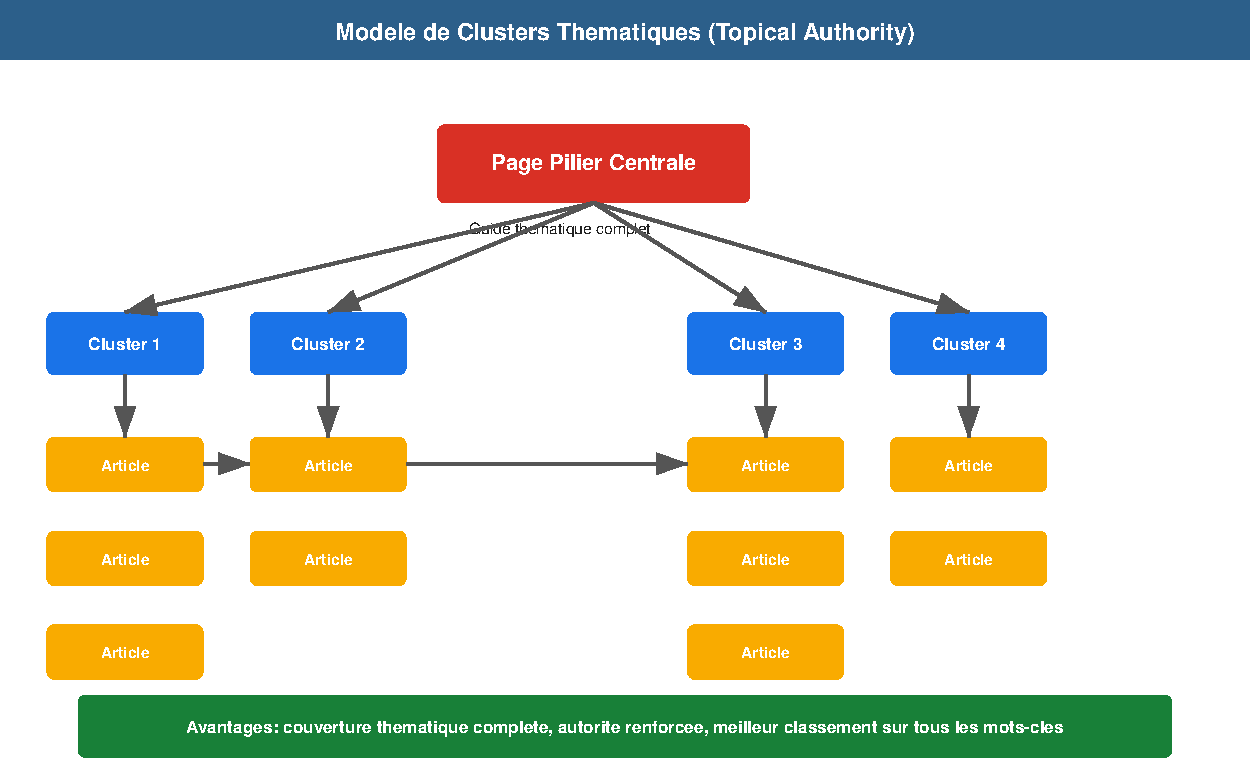
\includegraphics[width=\textwidth]{images/content_cluster.pdf}
    \caption{Modèle de clusters thématiques pour construire l'autorité et le topical authority}
    \label{fig:content_strategy}
\end{figure}

\section{Fondamentaux du Content Marketing SEO}

Le \keyword{Content Marketing SEO} est l'art de creer, distribuer et promouvoir du contenu dans le but d'attirer un trafic organique qualifie. Il ne s'agit plus simplement d'ecrire des articles de blog, mais de construire une \important{stratégie editoriale} complete alignee avec les objectifs business.

\subsection{Les piliers du Content Marketing SEO}

\begin{mybox}{Les 4 piliers du Content Marketing SEO}{googleblue}
\begin{enumerate}
    \item \textbf{Recherche} : Data-driven, basee sur l'intention de recherche et l'analyse concurrentielle
    \item \textbf{Creation} : Contenu de qualité répondant aux critères E-E-A-T
    \item \textbf{Distribution} : Promotion multi-canal pour maximiser la portee
    \item \textbf{Mesure} : ROI, KPIs, attribution et itération continue
\end{enumerate}
\end{mybox}

\section{Planification editoriale}

\subsection{Calendrier éditorial}

Le \keyword{calendrier éditorial} est un outil indispensable pour structurer la production de contenu :

\begin{itemize}
    \item \textbf{Periodicite} : Rythme de publication régulier (hebdomadaire, bi-mensuel)
    \item \textbf{Saisonnalite} : Contenu adapte aux cycles saisonniers du marché
    \item \textbf{Evenements} : Salons, conferences, actualites du secteur
    \item \textbf{Etapes du funnel} : Contenu pour chaque étape (TOFU, MOFU, BOFU)
    \item \textbf{Piliers thématiques} : Couverture cyclique des sujets principaux
    \item \textbf{Mise à jour} : Planning de rafraichissement du contenu existant
\end{itemize}

\subsection{Outils de planification}

\begin{itemize}
    \item \textbf{Trello / Asana} : Kanban pour le suivi de production
    \item \textbf{Notion} : Base de données editoriale complete
    \item \textbf{CoSchedule} : Calendrier éditorial avec intégration réseaux sociaux
    \item \textbf{ContentKing} : Monitoring et planification de mise à jour
    \item \textbf{Google Calendar} : Solution simple partagee en équipe
\end{itemize}

\section{Frameworks de contenu}

\subsection{Hub-and-Spoke (Pilier et clusters)}

Le modèle \keyword{Hub-and-Spoke} (ou Topic Cluster) est le framework le plus efficace pour le SEO :

\begin{itemize}
    \item \textbf{Page pilier} : Contenu long-form exhaustif sur un sujet principal ($\sim$3000--5000 mots)
    \item \textbf{Pages clusters} : Articles detailles sur des sous-sujets spécifiques ($\sim$1500--2500 mots)
    \item \textbf{Liens internes} : Tous les clusters pointent vers le pilier et vice-versa
    \item \textbf{Couverture sémantique} : Le cluster couvre l'intégralité du champ lexical du sujet
\end{itemize}

\begin{lstlisting}[style=htmlcode,caption={Structure Hub-and-Spoke pour le SEO}]
Page Pilier : "Guide complet du SEO en 2026"
  |
  |-- Cluster 1 : "Recherche de mots-clés"
  |     |-- Article : "Outils de keyword research"
  |     |-- Article : "Long-tail keywords"
  |     |-- Article : "Intentions de recherche"
  |
  |-- Cluster 2 : "SEO technique"
  |     |-- Article : "Core Web Vitals"
  |     |-- Article : "Indexation mobile-first"
  |     |-- Article : "Données structureées"
  |
  |-- Cluster 3 : "Netlinking"
  |     |-- Article : "Strategies de link building"
  |     |-- Article : "Backlinks dofollow vs nofollow"
  |
  |-- Cluster 4 : "SEO local"
        |-- Article : "Google Business Profile"
        |-- Article : "Citations NAP"
\end{lstlisting}

\subsection{Skyscraper Technique}

La \keyword{Skyscraper Technique}, popularisee par Brian Dean (Backlinko), repose sur trois étapes :

\begin{enumerate}
    \item \textbf{Trouver} : Identifiez un contenu performant dans votre niche (beaucoup de backlinks, bon trafic)
    \item \textbf{Ameliorer} : Creez une version plus complete, mieux structureé, plus visuelle, plus à jour
    \item \textbf{Promouvoir} : Contactez les sites qui linkent la version originale pour leur proposer votre version amélioree
\end{enumerate}

\important{La Skyscraper Technique peut générer 2 a 3 fois plus de backlinks que le contenu original.}

\subsection{Content Pillars}

Les \keyword{Content Pillars} sont les 3--5 sujets fondamentaux autour desquels s'articule toute la stratégie de contenu :

\begin{itemize}
    \item Chaque pilier représente un domaine d'expertise de l'entreprise
    \item Tous les contenus produits doivent se rattâcher à l'un de ces piliers
    \item Les piliers doivent correspondre aux mots-clés stratégiques
\end{itemize}

\section{Méthodologie de recherche de sujets}

\subsection{Analyse des SERP}

Avant de creer du contenu, analysez les \keyword{SERP} pour le mot-cle cible :

\begin{enumerate}
    \item \textbf{Type de contenu} : Blog, landing page, vidéo, e-commerce ?
    \item \textbf{Format dominant} : Listes, guides, tutoriels, comparatifs ?
    \item \textbf{Intention de recherche} : Informationnelle, navigationnelle, transactionnelle ?
    \item \textbf{Featured snippets} : Y a-t-il un extrait optimisable ?
    \item \textbf{Questions connexes} : "People Also Ask" pour enrichir le contenu
    \item \textbf{Autorite des concurrents} : Domain Authority des pages classees
    \item \textbf{Age du contenu} : Contenu récent ou obsolète ? Opportunité de mise à jour
\end{enumerate}

\subsection{Outils de recherche thématique}

\begin{itemize}
    \item \textbf{Ahrefs Content Explorer} : Trouver le contenu le plus partage par thématique
    \item \textbf{SEMrush Topic Research} : Idees de sujets avec score de potentiel
    \item \textbf{AnswerThePublic} : Questions posees par les utilisateurs
    \item \textbf{Google Trends} : Tendances et saisonnalité des sujets
    \item \textbf{AlsoAsked} : Arbre de questions connexes
    \item \textbf{Google Autocomplete} : Suggestions de recherche en temps réel
\end{itemize}

\subsection{Gap Analysis (Analyse des ecarts)}

Le \keyword{Content Gap Analysis} identifie les sujets que vos concurrents couvrent mais que vous ne couvrez pas :

\begin{enumerate}
    \item Lister vos 5 concurrents directs en SEO
    \item Exporter leurs URLs via Screaming Frog ou Ahrefs
    \item Analyser leurs mots-clés positionnés
    \item Comparer avec votre couverture thématique
    \item Identifier les sujets a forte opportunité (trafic $\times$ difficulte)
    \item Prioriser selon le potentiel business
\end{enumerate}

\section{Optimisation des formats de contenu}

\subsection{Contenu long-form ($>$ 2000 mots)}

Le contenu long-form tend a mieux performer dans les SERP :

\begin{itemize}
    \item \textbf{Guides complets} : Couverture exhaustive d'un sujet
    \item \textbf{Piliers de contenu} : 3000--5000 mots avec structure en sections
    \item \textbf{Whitepapers} : Contenu premium pour generation de leads
    \item \textbf{Etudes de cas} : Résultats concrets, data-driven
    \item \textbf{Comparatifs} : Analyse detaillee produit vs produit
\end{itemize}

\subsection{Contenu intermédiaire (1000--2000 mots)}

\begin{itemize}
    \item Articles de blog standard
    \item Tutoriels et how-to
    \item Listes et classements (Listicles)
    \item News et actualites du secteur
\end{itemize}

\subsection{Contenu court ($<$ 1000 mots)}

\begin{itemize}
    \item Fiches produits optimisées
    \item FAQ structureées (données structureées FAQ)
    \item Glossaires et définitions
    \item Micro-contenu pour réseaux sociaux
\end{itemize}

\section{Strategie de distribution de contenu}

Creer du contenu sans le distribuer, c'est comme organiser une fete sans invitér personne.

\subsection{Canaux de distribution}

\begin{enumerate}
    \item \textbf{Email marketing} : Newsletter vers votre base d'abonnes
    \item \textbf{Reseaux sociaux} : LinkedIn pour B2B, Instagram/TikTok pour B2C
    \item \textbf{Communautes} : Reddit, Quora, groupes Facebook, Slack/Discord
    \item \textbf{Medium / LinkedIn Articles} : Republishing avec canonical
    \item \textbf{Influenceurs} : Collaboration avec des experts du secteur
    \item \textbf{Digital PR} : Relations prèsse et publications invitées
    \item \textbf{Paid promotion} : Contenu sponsorise sur les réseaux
\end{enumerate}

\section{Repurposing de contenu}

Le \keyword{repurposing} (réutilisation) consiste a adapter un meme contenu sous différents formats :

\begin{itemize}
    \item Article de blog $\rightarrow$ Video YouTube + Podcast + Infographie + LinkedIn carousel
    \item Webinaire $\rightarrow$ Serie d'articles + Transcript + Clips vidéo
    \item Livre blanc $\rightarrow$ Landing page + Email sequence + SlideShare
    \item Etude de cas $\rightarrow$ Temoignage vidéo + Case study PDF + Post LinkedIn
    \item Podcast $\rightarrow$ Transcription SEO + Show notes + Clips sociaux
\end{itemize}

\begin{mybox}{Regle des 7 contacts}{googleyellow}
Un prospect a besoin de voir votre contenu en moyenne 7 fois avant de passer à l'action. Le repurposing permet de multiplier les points de contact avec un meme message sans effort de création supplementaire.
\end{mybox}

\section{Mesure du ROI du contenu}

\subsection{KPIs essentiels}

\begin{itemize}
    \item \textbf{Trafic organique} : Sessions provenant de la recherche Google
    \item \textbf{Mots-clés positionnés} : Nombre et évolution dans le top 3, top 10
    \item \textbf{Backlinks génères} : Nombre et qualité des liens entrants
    \item \textbf{Taux de conversion} : Leads, inscriptions, ventes attribues au contenu
    \item \textbf{Engagement} : Temps passe, pages par session, scroll depth
    \item \textbf{Brand awareness} : Recherches de marque, mentions sociales
    \item \textbf{Share of voice} : Visibilite par rapport aux concurrents
\end{itemize}

\subsection{Modeles d'attribution}

\begin{itemize}
    \item \textbf{First-click} : Attribue la conversion au premier point de contact
    \item \textbf{Last-click} : Attribue la conversion au dernier point de contact
    \item \textbf{Multi-touch} : Distribue le credit entre tous les points de contact
    \item \textbf{Data-driven} : Attribution algorithmique basee sur l'impact réel
\end{itemize}

\section{Analyse concurrentielle de contenu}

\subsection{Méthodologie}

\begin{enumerate}
    \item Identifiez vos concurrents SEO (pas seulement concurrents business)
    \item Analysez leur top contenu (Ahrefs / SEMrush Top Pages)
    \item Evaluez pour chaque page : trafic, backlinks, engagement, format
    \item Comparez avec vos performances
    \item Identifiez les gaps et opportunités
    \item Creez un plan d'action priorise
\end{enumerate}

\begin{lstlisting}[style=code,caption={Structure d'analyse concurrentielle (tableau de benchmark)}]
# Analyse concurrentielle de contenu
concurrents = [
    { "nom": "Concurrent A", "domaine": "concurrent-a.com",
      "top_pages": [
        {"url": "/guide-seo", "trafic": 15000, "backlinks": 450,
         "mots": 3200, "format": "guide"},
        {"url": "/outils-seo", "trafic": 12000, "backlinks": 280,
         "mots": 1800, "format": "liste"}
    ]},
    { "nom": "Concurrent B", "domaine": "concurrent-b.com",
      "top_pages": [
        {"url": "/formations-seo", "trafic": 8000, "backlinks": 120,
         "mots": 2500, "format": "page-cours"}
    ]}
]

# Calcul du score d'opportunité
def score_opportunité(trafic, backlinks, difficulte):
    return (trafic * 0.4 + backlinks * 10 * 0.3) / (difficulte + 1) * 100
\end{lstlisting}

% =============================================================================

% ============================================
% PARTIE 6 : SEO SPÉCIALISÉ
% ============================================

\part{Le SEO Spécialisé}
\label{part:specialise}

% ========== CHAPITRE 21 ==========
\begin{takeaways}
\begin{itemize}
    \item Le content marketing SEO vise à attirer du trafic qualifié via le contenu
    \item La structure hub-and-spoke organise le contenu autour de piliers thématiques
    \item Le ROI du contenu se mesure par des KPIs précis et des modèles d'attribution
\end{itemize}
\end{takeaways}

\level{2}
\begin{objectives}
\begin{itemize}
    \item Comprendre l'importance du SEO local
    \item Maîtriser Google Business Profile
    \item Gérer les citations NAP et annuaires
\end{itemize}
\end{objectives}

\chapter{Le SEO Local}
\label{ch:localseo}

\begin{figure}[H]
    \centering
    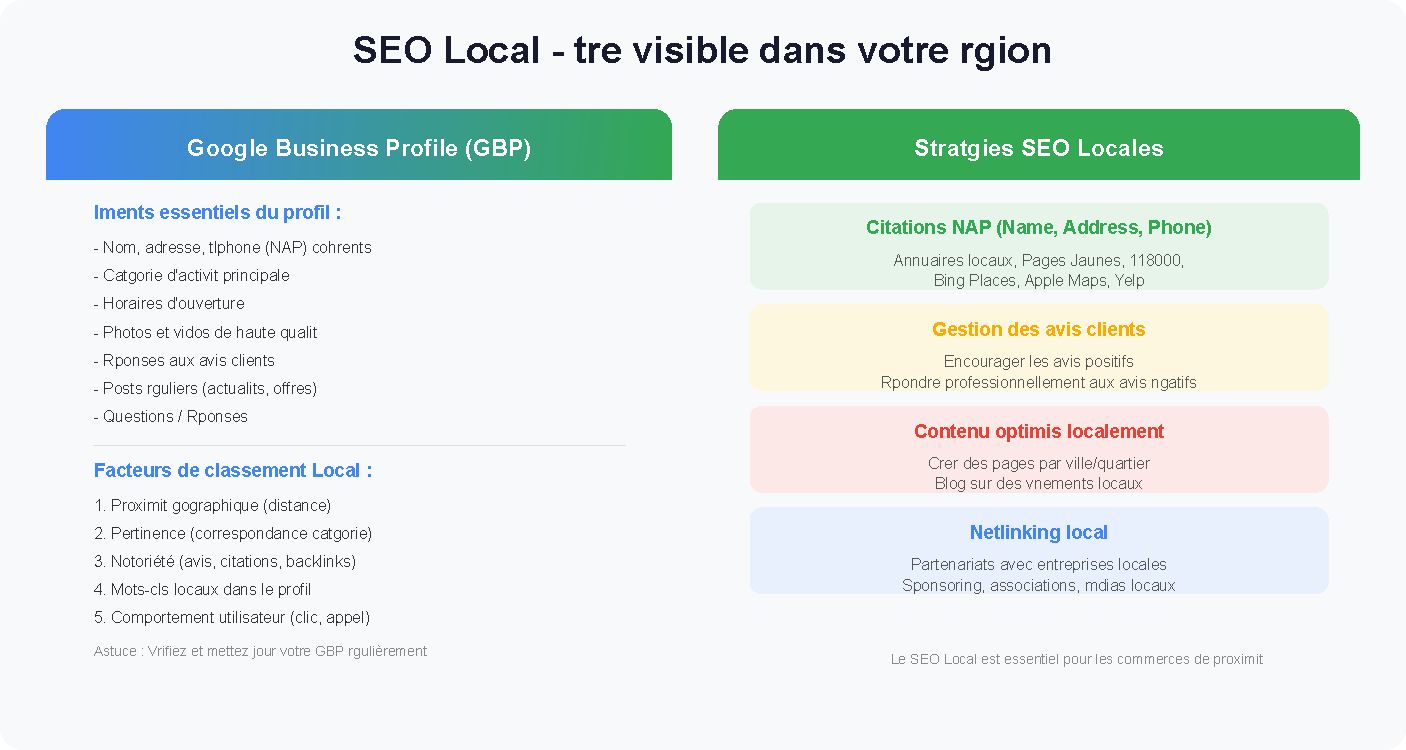
\includegraphics[width=\textwidth]{images/seo_local.pdf}
    \caption{Facteurs de classement du SEO local et optimisation Google Business Profile}
    \label{fig:local_seo}
\end{figure}

\section{L'importance du SEO Local}

Le \keyword{SEO local} est essentiel pour les entreprises ayant une présence physique. 46\% de toutes les recherches Google ont une intention locale, et 76\% des personnes qui effectuent une recherche locale visitent un magasin dans la journée. Les recherches \og près de moi\fg{} ont connu une croissance de plus de 500\% au cours des dernières années. Le Local Pack --- les trois résultats géolocalisés affichés en tête des SERP --- est devenu l'un des espaces les plus convoités du référencement.

\section{Google Business Profile (GBP)}

L'outil le plus important pour le SEO local est \keyword{Google Business Profile} (anciennement Google My Business). Un profil optimisé est un prérequis pour apparaître dans le Local Pack et sur Google Maps.

\subsection{Optimisation complète du profil GBP}

Un profil GBP parfaitement optimisé doit comporter :

\begin{itemize}
    \item \textbf{Informations NAP} (Name, Address, Phone) rigoureusement exactes et cohérentes sur toutes les plateformes
    \item \textbf{Catégorie d'activité} : sélectionnez la catégorie principale la plus pertinente et jusqu'à 10 catégories secondaires
    \item \textbf{Horaires d'ouverture} précis, incluant les jours fériés et les horaires exceptionnels
    \item \textbf{Photos et vidéos} : au moins 30 photos de haute qualité (extérieur, intérieur, équipe, produits)
    \item \textbf{Attributs} : WiFi, accès handicapés, parking, services proposés
    \item \textbf{Description d'activité} : 750 caractères maximisant les mots-clés locaux pertinents
    \item \textbf{Posts réguliers} : actualités, offres spéciales, événements (au moins 1 par semaine)
    \item \textbf{Section Questions/Réponses} : anticipez et renseignez les questions fréquentes
    \item \textbf{Produits et services} : catalogue complet directement dans le profil
\end{itemize}

\begin{mybox}{Astuce avancée GBP}{googlegreen}
Utilisez les \keyword{GBP Insights} pour identifier les mots-clés qui génèrent des vues sur votre profil. Publiez des posts avec des offres limitées dans le temps pour augmenter l'engagement et le taux de clics. Les profils avec des photos récentes reçoivent 42\% de demandes d'itinéraire en plus.
\end{mybox}

\subsection{GBP Insights et analyse des performances}

Les \keyword{GBP Insights} fournissent des données précieuses :

\begin{itemize}
    \item \textbf{Recherches} : requêtes utilisées pour trouver votre établissement (directes, de découverte, par marque)
    \item \textbf{Vues} : nombre de fois que votre profil est consulté sur Google Search et Maps
    \item \textbf{Actions} : clics vers le site web, demandes d'itinéraire, appels téléphoniques
    \item \textbf{Conversations} : messages échangés avec les clients via la messagerie GBP
    \item \textbf{Réservations} : clics sur les boutons de réservation (si applicable)
\end{itemize}

\section{Les facteurs de classement du Local Pack}

Le \keyword{Local Pack} de Google est influencé par trois catégories principales de facteurs :

\begin{enumerate}
    \item \textbf{Pertinence} : adéquation entre le profil GBP et la requête de l'utilisateur (catégories, mots-clés, description)
    \item \textbf{Proximité} : distance entre l'établissement et la position de l'utilisateur ou le centre de la recherche
    \item \textbf{Notoriété} : popularité de l'établissement (avis, citations, backlinks locaux, autorité globale)
\end{enumerate}

D'autres facteurs secondaires incluent la complétude du profil GBP, la régularité des posts, la vitesse de réponse aux avis et la cohérence NAP sur le web.

\section{Les données structurées locales (LocalBusiness Schema)}

Le \keyword{schema LocalBusiness} permet d'envoyer des signaux forts à Google sur la nature locale de votre activité :

\begin{lstlisting}[style=htmlcode,caption={Exemple de LocalBusiness Schema Markup}]
<script type="application/ld+json">
{
  "@context": "https://schema.org",
  "@type": "Restaurant",
  "name": "Bistrot Parisien",
  "image": "https://example.com/photo.jpg",
  "url": "https://example.com",
  "telephone": "+33123456789",
  "address": {
    "@type": "PostalAddress",
    "streetAddress": "15 Rue de la Paix",
    "addressLocality": "Paris",
    "addressRegion": "Île-de-France",
    "postalCode": "75002",
    "addressCountry": "FR"
  },
  "geo": {
    "@type": "GeoCoordinates",
    "latitude": 48.8698,
    "longitude": 2.3312
  },
  "openingHoursSpecification": [
    {
      "@type": "OpeningHoursSpecification",
      "dayOfWeek": ["Monday","Tuesday"],
      "opens": "09:00",
      "closes": "18:00"
    }
  ],
  "aggregateRating": {
    "@type": "AggregateRating",
    "ratingValue": "4.5",
    "reviewCount": "250"
  }
}
</script>
\end{lstlisting}

\important{Le schema LocalBusiness doit être implémenté sur la page contact de votre site. Pour les établissements multi-sites, utilisez le type \texttt{AggregateOffer} ou créez une page par établissement avec son propre schema.}

\section{Les citations NAP et la gestion des annuaires}

La \keyword{consistance NAP} (même nom, même adresse, même téléphone sur tous les annuaires) est un facteur de classement local fondamental. Google recoupe ces informations pour valider la légitimité de votre entreprise.

\subsection{Stratégie de création de citations}

\begin{enumerate}
    \item \textbf{Annuaires généralistes} : PagesJaunes, 118000, Kompass, Bing Places, Apple Maps
    \item \textbf{Annuaires internationaux} : Yelp, TripAdvisor, Foursquare, Infobel, Europages
    \item \textbf{Annuaires sectoriels} : référencement spécialisé par métier (avocats, santé, restauration, etc.)
    \item \textbf{Data aggregators} : Infogreffe, Société.com, SIRENE (base INSEE)
\end{enumerate}

\begin{toolsbox}
Outils de gestion des citations : \keyword{Yext} (automatisation multi-annuaires), \keyword{BrightLocal} (audit et suivi NAP), \keyword{Whitespark} (découverte de nouvelles opportunités de citations), \keyword{Moz Local} (vérification de cohérence).
\end{toolsbox}

\section{Stratégie de gestion des avis clients}

Les avis clients sont un facteur de ranking et un levier de conversion majeur :

\begin{itemize}
    \item \textbf{Quantité} : encouragez systématiquement les clients satisfaits à laisser un avis (QR code, email post-achat)
    \item \textbf{Qualité} : les avis détaillés avec photos ont plus de poids
    \item \textbf{Diversité} : collectez des avis sur Google, TripAdvisor, Yelp et les plateformes sectorielles
    \item \textbf{Réponses} : répondez à 100\% des avis --- remerciez les avis positifs en 24h, traitez les négatifs avec professionnalisme
\end{itemize}

\section{Le netlinking local}

Les backlinks locaux renforcent l'autorité géographique :

\begin{itemize}
    \item \textbf{Chambres de commerce} : adhésion et inscription dans les annuaires de la CCI
    \item \textbf{Partenariats locaux} : échanges de liens avec des entreprises complémentaires de la même zone
    \item \textbf{Événements locaux} : sponsoring, participation et articles de presse locale
    \item \textbf{Médias locaux} : relations presse avec les journaux et blogs de quartier
    \item \textbf{Associations professionnelles} : adhésion aux organisations professionnelles régionales
\end{itemize}

\section{SEO pour les établissements multi-sites}

Pour les chaînes ou franchises avec plusieurs établissements :

\begin{enumerate}
    \item Créez un profil GBP distinct pour chaque emplacement physique
    \item Utilisez une page dédiée par établissement sur votre site (avec schema LocalBusiness unique)
    \item Assurez-vous que chaque page contient le NAP spécifique au site concerné
    \item Évitez les contenus dupliqués entre les pages des différents établissements
    \item Personnalisez les descriptions avec des éléments propres à chaque emplacement (quartier, spécificités locales)
\end{enumerate}

\section{Stratégie de contenu local}

Le contenu géolocalisé renforce la pertinence locale :

\begin{itemize}
    \item \textbf{Pages quartier} : créez du contenu spécifique à chaque zone géographique desservie
    \item \textbf{Actualités locales} : articles sur des événements, actualités ou tendances locales
    \item \textbf{Guides locaux} : \og Que faire dans [ville]\fg{} ou \og Guide du [quartier]\fg{}
    \item \textbf{Témoignages clients} : études de cas avec des clients locaux identifiés
\end{itemize}

\section{Étude de cas : Campagne SEO local pour un réseau de boulangeries}

\textbf{Contexte :} Un réseau de 15 boulangeries artisanales en Île-de-France souhaitait augmenter le trafic piéton de 40\%.

\textbf{Stratégie mise en œuvre :}
\begin{itemize}
    \item Optimisation complète des 15 profils GBP (photos professionnelles, horaires, attributs)
    \item Création de pages de quartier uniques avec schema LocalBusiness par établissement
    \item Campagne de collecte d'avis (QR code sur les emballages, +150 avis en 3 mois)
    \item Citations NAP sur 45 annuaires via Yext
    \item Articles sponsorisés dans 5 journaux de quartier
\end{itemize}

\textbf{Résultats :}
\begin{itemize}
    \item Apparition dans le Local Pack pour 12 des 15 établissements
    \item +65\% de trafic piéton (objectif initial : +40\%)
    \item Note moyenne GBP passée de 4,1 à 4,7 étoiles
    \item +120\% de clics vers le site web depuis les profils GBP
\end{itemize}

\begin{takeaways}
\begin{itemize}
    \item Le SEO local est essentiel pour les commerces de proximité
    \item Google Business Profile est l'outil central du SEO local
    \item La cohérence NAP est cruciale pour la confiance des moteurs
    \item Les avis clients influencent le classement et la conversion
    \item Le schema LocalBusiness renforce les signaux géographiques
\end{itemize}
\end{takeaways}

\level{3}
\begin{objectives}
\begin{itemize}
    \item Comprendre les différents types de migration
    \item Maîtriser la stratégie de redirection 301
    \item Savoir gérer une migration de A à Z
\end{itemize}
\end{objectives}

\chapter{Migration SEO et Redirection}
\label{ch:migration}

\section{Introduction aux migrations SEO}

Une \keyword{migration SEO} est tout changement significatif apporte à un site web qui peut impacter sa visibilité dans les moteurs de recherche. Les migrations sont des moments \important{critiques} : une mauvaise execution peut faire perdre des annees de travail SEO en quelques jours.

\subsection{Types de migrations}

\begin{itemize}
    \item \textbf{Migration de domaine} : Changement de nom de domaine
    \item \textbf{Migration de protocole} : HTTP $\rightarrow$ HTTPS
    \item \textbf{Migration de CMS} : Passage d'un CMS à un autre
    \item \textbf{Migration de structure} : Changement d'URLs, d'architecture de site
    \item \textbf{Migration de design} : Refonte visuelle majeure
    \item \textbf{Migration de serveur} : Changement d'hebergement ou de CDN
    \item \textbf{Migration de plateforme} : Passage d'une plateforme à une autre
\end{itemize}

\section{Checklist pré-migration}

\subsection{Audit pré-migration (\important{avant})}

\begin{enumerate}
    \item \textbf{Backup complet} : Base de données, fichiers, configuration serveur
    \item \textbf{Inventaire des URLs} : Crawl complet avec Screaming Frog / Sitebulb
    \item \textbf{Mapping URL complet} : Table de correspondance ancienne $\rightarrow$ nouvelle URL
    \item \textbf{Benchmark des performances} : Trafic, positions, conversions (minimum 3 mois)
    \item \textbf{Rapport Core Web Vitals} : LCP, INP, CLS avant migration
    \item \textbf{Indexation} : Nombre de pages indexees dans GSC
    \item \textbf{Backlinks} : Export des backlinks (Ahrefs, Majestic)
    \item \textbf{Sitemap} : Sitemap XML actuel complet
    \item \textbf{Robots.txt} : Etat actuel
    \item \textbf{Redirections existantes} : Inventaire des 301 en place
\end{enumerate}

\begin{mybox}{Outil recommandé pour le mapping URL}{googleblue}
Utilisez \textbf{Screaming Frog SEO Spider} avec la fonction "Export All URLs" puis importez le fichier CSV dans un tableur pour creer le mapping colonne par colonne : Ancienne URL $\rightarrow$ Nouvelle URL $\rightarrow$ Type de redirection $\rightarrow$ Statut.
\end{mybox}

\section{Strategie de redirection : 301 vs 302}

\subsection{HTTP 301 -- Redirection permanente}

Le code \keyword{301} (Moved Permanently) transmet 90--99\% du PageRank (Google) :

\begin{itemize}
    \item \textbf{Usage} : Changement permanent d'URL
    \item \textbf{Transmission SEO} : Transmet la majorite de l'autorite et du ranking
    \item \textbf{Mise à jour de l'index} : Google remplace l'ancienne URL par la nouvelle
    \item \textbf{Delai} : 1--3 mois pour la transmission complete du PageRank
\end{itemize}

\subsection{HTTP 302 -- Redirection temporaire}

Le code \keyword{302} (Found / Temporarily Redirect) ne transmet pas l'autorite :

\begin{itemize}
    \item \textbf{Usage} : Test A/B, page en maintenance, contenu saisonnier
    \item \textbf{Transmission SEO} : Google conserve l'ancienne URL comme canonique
    \item \textbf{Attention} : Google interprete parfois les 302 repetes comme des 301
    \item \textbf{Deconseille pour} : Les migrations permanentes
\end{itemize}

\subsection{Autrès codes de redirection}

\begin{itemize}
    \item \textbf{307} : Redirection temporaire, meme méthode HTTP (remplacement moderne du 302)
    \item \textbf{308} : Redirection permanente, meme méthode HTTP (remplacement moderne du 301)
    \item \textbf{303} : See Other, utilise après un POST pour éviter la re-soumission
\end{itemize}

\subsection{Regles de redirection}

\begin{lstlisting}[style=code,caption={Fichier de redirection NGINX pour migration massive}]
# Mapping des redirections 301 (fichier de configuration NGINX)
# Ancien site -> Nouveau site

# Pages principales
rewrite ^/ancien-produit-1$ /nouveau-produit-1 permanent;
rewrite ^/ancien-produit-2$ /nouveau-produit-2 permanent;
rewrite ^/catégorie/ancienne-cat$ /nouvelle-catégorie/ permanent;

# Redirection par pattern (catégories avec ID)
rewrite ^/cat-([0-9]+)/(.*)$ /catégorie/$1/$2 permanent;

# Redirection des articles de blog (date vers slug)
rewrite ^/blog/([0-9]{4})/([0-9]{2})/(.*)$
        /blog/$3 permanent;

# Redirection des images
rewrite ^/images/ancien/(.*)$ /images/$1 permanent;
\end{lstlisting}

\section{Mapping URL : méthodologie}

Le \keyword{URL mapping} est la pièce maîtrèsse d'une migration réussie :

\subsection{Processus de mapping}

\begin{enumerate}
    \item Crawlez l'ancien site avec Screaming Frog (export CSV complet)
    \item Classez les URLs par priorité (trafic, backlinks, conversions)
    \item Creez la correspondance pour chaque URL vers la nouvelle structure
    \item Pour les URLs sans équivalent : 301 vers la page parente la plus proche
    \item Evitez le 301 général vers la home page (considéré comme soft 404)
    \item Testez les redirections en staging avant le déploiement
    \item Validez avec un outil de vérification de redirections
\end{enumerate}

\begin{lstlisting}[style=code,caption={Script de vérification des redirections avec Python}]
import requests

def check_redirects(csv_file):
    with open(csv_file, 'r') as f:
        for line in f:
            old_url, expected_new_url = line.strip().split(',')

            try:
                response = requests.get(
                    old_url,
                    allow_redirects=True,
                    timeout=10
                )

                final_url = response.url.rstrip('/')

                if response.status_code == 200 and final_url == expected_new_url:
                    print(f"[OK] {old_url} -> {final_url}")
                elif response.status_code == 404:
                    print(f"[ERREUR 404] {old_url}")
                elif response.status_code in [301, 302]:
                    print(f"[REDIRECT] {old_url} -> {response.headers.get('Location', 'N/A')}")
                else:
                    print(f"[STATUS {response.status_code}] {old_url}")

            except Exception as e:
                print(f"[EXCEPTION] {old_url} : {e}")

check_redirects('url_mapping.csv')
\end{lstlisting}

\section{Gestion des DNS}

\subsection{Plan de changement DNS}

\begin{enumerate}
    \item \textbf{TTL bas} : Reduisez le TTL a 300 secondes (5 min) au moins 48h avant
    \item \textbf{Preparez les enregistrements} : A, CNAME, MX, TXT, DKIM, SPF, DMARC
    \item \textbf{Changez les DNS} : Tot le matin ou en période de faible trafic
    \item \textbf{Verifiez la propagation} : \texttt{dig} ou outils en ligne (whatsmydns.net)
    \item \textbf{Surveillez} : Propagation complete en 24--72h
    \item \textbf{Retablissez le TTL} : Remettez le TTL à sa valeur normale (3600+)
\end{enumerate}

\important{Ne changez jamais vos DNS pendant une période de forte activite commerciale (Noel, Black Friday, soldes).}

\section{Test en environnement de staging}

Avant de déployer, il est \important{impératif} de tester dans un environnement isolé :

\begin{enumerate}
    \item \textbf{Protection du staging} : Mot de passe ou IP restriction pour éviter l'indexation
    \item \textbf{Test des redirections} : Automatise avec scripts
    \item \textbf{Test des URLs} : Toutes les pages sont accèssibles sans erreur
    \item \textbf{Test du sitemap} : Valide et soumis
    \item \textbf{Test du robots.txt} : Correct, ne bloque pas les ressources essentielles
    \item \textbf{Test des données structureées} : Schema.org valide (Rich Results Test)
    \item \textbf{Test des balises meta} : Title, description, canonical, hreflang
    \item \textbf{Test mobile} : Mobile-friendly, responsive
    \item \textbf{Test de vitesse} : Performance équivalente ou meilleure
    \item \textbf{Test fonctionnel} : Formulaires, panier, paiement, recherche
\end{enumerate}

\section{Post-migration : monitoring}

\subsection{Jour de la migration}

\begin{itemize}
    \item \textbf{Redirection} : Activez les 301 des le basculement DNS
    \item \textbf{Sitemap} : Soumettez le nouveau sitemap dans GSC
    \item \textbf{Demande d'indexation} : URLs critiques via GSC "Inspecter une URL"
    \item \textbf{Annonce} : Informez Google via le changement d'adresse dans GSC
    \item \textbf{Surveillance en temps réel} : Logs serveur, erreurs 404, 500
\end{itemize}

\subsection{Suivi a 1 semaine}

\begin{itemize}
    \item \textbf{Indexation} : Verifiez le nombre de pages indexees
    \item \textbf{Erreurs 404} : Corrigez les redirections manquantes
    \item \textbf{Trafic} : Comparez avec la semaine pré-migration
    \item \textbf{Positions} : Verifiez les mots-clés principaux
    \item \textbf{Core Web Vitals} : Impact sur les performances
\end{itemize}

\subsection{Suivi a 1 mois}

\begin{itemize}
    \item \textbf{Backlinks} : Verifiez la transmission via les nouveaux URLs
    \item \textbf{Trafic global} : Doit etre a 80--100\% du niveau pré-migration
    \item \textbf{Conversions} : Doivent revenir au niveau précédent
    \item \textbf{Rapport de couverture GSC} : Analyser les erreurs
\end{itemize}

\subsection{Suivi a 3 mois}

\begin{itemize}
    \item \textbf{Transmission SEO complete} : Le trafic devrait etre stabilise
    \item \textbf{Si le trafic n'est pas revenu} : Audit des causes possibles
    \item \textbf{Optimisations post-migration} : Ameliorations continues
\end{itemize}

\begin{mybox}{Indicateurs clés post-migration}{googlered}
Surveillez ces métriques quotidiennement pendant les 2 premières semaines :
\begin{itemize}
    \item \textbf{404 en hausse} $\rightarrow$ Redirections manquantes
    \item \textbf{Baisse du crawl Googlebot} $\rightarrow$ Probleme technique
    \item \textbf{Baisse du CTR} $\rightarrow$ Titrès/descriptions mal migres
    \item \textbf{Baisse des pages indexees} $\rightarrow$ Noindex ou canonical errone
    \item \textbf{Augmentation du TTFB} $\rightarrow$ Probleme de performance
\end{itemize}
\end{mybox}

\section{Plan de rollback}

Toute migration doit inclure un \important{plan de retour arriere} :

\begin{enumerate}
    \item \textbf{Snapshot complet} avant la migration (base de données + fichiers)
    \item \textbf{Sauvegarde de l'ancien site} : Serveur complet, intact
    \item \textbf{Script de rollback} : Pret à être execute en $<$ 30 minutes
    \item \textbf{Conditions de rollback} : Definir les seuils (ex: -30\% de trafic en 48h)
    \item \textbf{Communication} : Qui prevenir, comment annoncer le rollback
    \item \textbf{Test du plan} : Simuler le rollback en staging
\end{enumerate}

\section{Pieges fréquents des migrations}

\begin{mybox}{Top 10 des erreurs de migration}{googlered}
\begin{enumerate}
    \item \textbf{Absence de mapping URL} : Redirections génériques vers la home page
    \item \textbf{Melange 301/302} : Utilisation incorrecte des codes de redirection
    \item \textbf{Chaines de redirection} : A $\rightarrow$ B $\rightarrow$ C au lieu de A $\rightarrow$ C
    \item \textbf{Boucles de redirection} : A $\rightarrow$ B $\rightarrow$ A
    \item \textbf{Noindex accidentel} : Balise noindex oubliée sur le nouveau site
    \item \textbf{Canonical incorrect} : Canonical pointant vers l'ancienne version
    \item \textbf{Robots.txt bloquant} : Disallow sur les ressources CSS/JS/images
    \item \textbf{Changement DNS trop rapide} : TTL insuffisant pour la propagation
    \item \textbf{Absence de test mobile} : Nouveau site non responsive
    \item \textbf{Perte des données utilisateur} : Comptes, historiques, paniers non migres
\end{enumerate}
\end{mybox}

\section{Etude de cas : Migration réussie}

\subsection{Cas pratique : Migration HTTP $\rightarrow$ HTTPS + changement de domaine}

\textbf{Contexte :} Site e-commerce avec 50 000 pages, 200 000 visiteurs/mois.

\textbf{Preparation :}
\begin{itemize}
    \item 2 mois de préparation (audit, mapping, tests)
    \item Redirection 301 individualisee pour chaque URL
    \item Conservation de la structure d'URL
    \item TTL DNS réduit a 300s une semaine avant
\end{itemize}

\textbf{Résultats :}
\begin{itemize}
    \item Trafic inchangé a J+7 (--2\%)
    \item Positions conservees a J+14
    \item Backlinks transmis a 95\% a M+2
    \item Amelioration du CTR grâce au cadenas HTTPS (+3\%)
\end{itemize}

\important{Une migration preparee sur 2 mois avec un mapping URL exhaustif a permis de ne perdre quasiment aucun trafic.}

% =============================================================================

% ========== CHAPITRE 22 ==========
\begin{takeaways}
\begin{itemize}
    \item Les migrations de site présentent des risques SEO importants
    \item Un mapping URL complet est indispensable avant la migration
    \item Le suivi post-migration sur 3 mois est nécessaire
\end{itemize}
\end{takeaways}

\level{2}
\begin{objectives}
\begin{itemize}
    \item Identifier les défis spécifiques du SEO e-commerce
    \item Optimiser l'architecture d'un site e-commerce
    \item Éviter les pièges du contenu duplicate
\end{itemize}
\end{objectives}

\chapter{Le SEO pour l'E-commerce}
\label{ch:ecommerce}

\section{Défis spécifiques du SEO e-commerce}

Le SEO pour les sites e-commerce présente des défis uniques qui le distinguent radicalement du SEO pour les sites vitrine ou les blogs :

\begin{itemize}
    \item \textbf{Grande quantité de pages} : Des milliers voire des millions de fiches produits, catégories, filtres et pages de marques
    \item \textbf{Contenu dupliqué} : Descriptions fournisseurs réutilisées, variations de produits, pages de filtres redondantes
    \item \textbf{Depth de crawl} : Les ressources de crawl doivent être réparties entre des milliers d'URLs
    \item \textbf{Pagination} : Gestion des pages de listing et de résultats de recherche interne
    \item \textbf{Filtres et facettes} : Génération d'URLs infinies et de contenu dupliqué
    \item \textbf{Produits hors stock} : Gestion des indisponibilités et des pages orphelines
    \item \textbf{Saisonnalité} : Produits saisonniers, soldes, arrivages --- contenu temporaire
\end{itemize}

\section{Optimisation des pages produits}

La \keyword{page produit} est l'unité centrale du SEO e-commerce. Chaque fiche doit être optimisée individuellement.

\subsection{Balises title et meta descriptions}

\begin{mybox}{Structure de title produit}{googleblue}
\texttt{[Nom du produit] -- [Caractéristique clé] | [Marque] -- [Site]}
\textbf{Exemple :} Chaussure de running Trail Ultralight -- Amorti maximal | Asics -- SportPlus
\end{mybox}

Chaque title doit contenir le mot-clé principal du produit, la marque, et un différenciateur. Évitez les titres génériques du type \texttt{Produit 123 | MonSite}.

\subsection{Données structurées produit}

Le \keyword{Product schema} est indispensable pour générer les rich snippets avec prix et disponibilité :

\begin{lstlisting}[style=htmlcode,caption={Schema Product avec offre et avis}]
<script type="application/ld+json">
{
  "@context": "https://schema.org",
  "@type": "Product",
  "name": "Chaussure Running Trail Ultralight",
  "description": "Chaussure de trail légère avec amorti maximal",
  "sku": "RUN-TRL-001",
  "brand": { "@type": "Brand", "name": "Asics" },
  "offers": [{
    "@type": "Offer",
    "price": "129.90",
    "priceCurrency": "EUR",
    "availability": "https://schema.org/InStock",
    "priceValidUntil": "2026-12-31"
  }],
  "aggregateRating": {
    "@type": "AggregateRating",
    "ratingValue": "4.6",
    "reviewCount": "89"
  }
}
</script>
\end{lstlisting}

\important{L'implémentation du schema Product avec l'offre et le prix à jour est un signal fort pour Google Shopping et les rich snippets. Vérifiez que le prix affiché dans le schema correspond exactement au prix visible sur la page.}

\section{Optimisation des pages catégories}

Les pages de \keyword{catégorie} sont souvent les portes d'entrée principales pour le trafic e-commerce.

\begin{enumerate}
    \item \textbf{Title et H1} : incluez le mot-clé de catégorie principal (ex : \og Chaussures de running homme\fg)
    \item \textbf{Description unique} : rédigez 150-300 mots décrivant la sélection, les critères de choix, les conseils
    \item \textbf{Texte éditorial} : évitez les descriptions génériques du type \og Découvrez notre sélection\fg
    \item \textbf{Filtres et tris} : utilisez des paramètres d'URL cohérents (ex : \texttt{?taille=M\&couleur=rouge})
    \item \textbf{Breadcrumbs} : structure de navigation hiérarchique avec schema BreadcrumbList
\end{enumerate}

\section{Navigation à facettes et gestion des paramètres}

La \keyword{ navigation à facettes} (filtres par taille, couleur, prix, marque) génère potentiellement des millions d'URLs.

\subsection{Bonnes pratiques}

\begin{itemize}
    \item \textbf{Noindex les URLs de filtre combiné} : utilisez la balise \texttt{<meta name="robots" content="noindex, follow">} sur les pages de filtres trop spécifiques
    \item \tag{Canonical} : faites pointer les URLs de filtre vers la page de catégorie parente
    \item \textbf{Ajax et lazy-loading} : chargez les résultats de filtre via JavaScript pour éviter la création d'URLs
    \item \textbf{Paramètres dans Google Search Console} : déclarez les paramètres d'URL (\texttt{?couleur=}, \texttt{?taille=}) comme \og ne modifie pas le contenu\fg ou \og modifie le contenu\fg selon le cas
    \item \textbf{Disallow sélectif dans robots.txt} : empêchez le crawl des combinaisons de filtres non pertinentes
\end{itemize}

\section{Gestion du contenu dupliqué}

Le contenu dupliqué est le fléau du SEO e-commerce. Les sources principales :

\begin{itemize}
    \item \textbf{Descriptions fournisseurs} : des centaines de revendeurs utilisent le même texte --- réécrivez systématiquement
    \item \textbf{Variantes de produits} : une balise canonical pointant vers la variante principale
    \item \textbf{Pages imprimable ou PDF} : noindex ou canonical vers la page originale
    \item \textbf{Session IDs et paramètres de tracking} : empêchez l'indexation via robots.txt ou canonical
    \item \textbf{Pagination} : balises \texttt{rel="prev"} et \texttt{rel="next"} ou configuration \og view-all\fg
\end{itemize}

\section{Google Shopping et flux produits}

L'intégration avec \keyword{Google Shopping} via un flux Merchant Center est complémentaire au SEO :

\begin{itemize}
    \item Le flux doit contenir : title, description, prix, disponibilité, GTIN/MPN, image link, Google Product Category
    \item Les données du flux doivent correspondre exactement au contenu de la page produit (price matching)
    \item Les avis produits (Product Ratings) augmentent le CTR dans Google Shopping
    \item Les promotions (soldes, livraison gratuite) apparaissent via le flux Merchant Center
\end{itemize}

\section{Architecture et profondeur de site}

Une \keyword{architecture e-commerce} optimale suit ces principes :

\begin{lstlisting}[style=htmlcode,caption={Architecture e-commerce à profondeur limitée (3 clics max)}]
Accueil (/)
  |-- Categorie N1 (/vetements/)
  |     |-- Sous-catégorie (/vetements/homme/)
  |     |     |-- Fiche Produit (/vetements/homme/t-shirt-coton-bio.html)
  |-- Categorie N1 (/chaussures/)
  |     |-- Sous-catégorie (/chaussures/running/)
  |     |     |-- Fiche Produit (/chaussures/running/asics-trail.html)
  |-- Marques (/marques/)
  |-- Blog (/blog/) [contenu informatif et guide d'achat]
\end{lstlisting}

\begin{mybox}{Règle des 3 clics}{googleyellow}
Toute page produit doit être accessible en 3 clics maximum depuis la page d'accueil. Une profondeur excessive dilue le PageRank et réduit le crawl budget alloué aux pages importantes.
\end{mybox}

\section{Pagination et view-all}

Pour les pages de listing avec plusieurs pages de résultats :

\begin{itemize}
    \item \textbf{rel="next" / rel="prev"} : indiquez la relation entre les pages de la série (bien que Google ait annoncé ne plus utiliser ces balises, elles restent une bonne pratique)
    \item \textbf{View-all page} : créez une page unique listant tous les produits de la catégorie --- si elle dépasse 10 000 produits, noindexez-la
    \item \textbf{Infinite scroll} : assurez-vous que le contenu chargé dynamiquement est crawlable (history.pushState pour mettre à jour l'URL)
\end{itemize}

\section{Étude de cas : SEO e-commerce pour un site de mobilier}

\textbf{Contexte :} Site e-commerce de mobilier avec 12 000 références, 80 000 pages indexées, dont 45\% de contenu dupliqué (descriptions fournisseurs).

\textbf{Problèmes identifiés :}
\begin{itemize}
    \item Descriptions fournisseurs identiques pour 5 400 produits
    \item 15 000 URLs de filtres indexées (taille, couleur, matière)
    \item Pages catégories sans texte éditorial
    \item Temps de chargement moyen de 4,2 secondes
\end{itemize}

\textbf{Actions mises en œuvre :}
\begin{itemize}
    \item Réécriture de 5 400 descriptions produits (contenu unique, 150 mots minimum)
    \item Noindex des URLs de filtres combinés, canonical vers la catégorie parente
    \item Ajout de guides d'achat sur les 25 pages catégories principales
    \item Optimisation Core Web Vitals (passage à 2,1 secondes de chargement)
\end{itemize}

\textbf{Résultats :}
\begin{itemize}
    \item Trafic organique : +78\% en 6 mois
    \item Pages indexées pertinentes : de 80 000 à 12 500 (qualité sur quantité)
    \item Taux de conversion SEO : +23\%
    \item Position moyenne des pages catégories : de 11,2 à 4,8
\end{itemize}

\begin{takeaways}
\begin{itemize}
    \item Le contenu dupliqué est un défi majeur pour l'e-commerce
    \item L'architecture du site doit privilégier la profondeur limitée
    \item Les fiches produits doivent contenir du contenu unique et des données structurées
    \item La navigation à facettes nécessite une gestion rigoureuse des paramètres
    \item Google Shopping et le SEO organique sont complémentaires
\end{itemize}
\end{takeaways}

\level{2}
\begin{objectives}
\begin{itemize}
    \item Connaître les spécificités SEO de chaque CMS
    \item Configurer correctement les plugins SEO
    \item Optimiser la performance par CMS
\end{itemize}
\end{objectives}

\chapter{SEO pour les CMS populaires}
\label{ch:cmsseo}

\section{WordPress SEO}

\keyword{WordPress} est le CMS le plus utilise au monde (43\% des sites web). Sa flexibilite en fait une plateforme de choix pour le SEO.

\subsection{Plugins SEO recommandés}

\begin{itemize}
    \item \textbf{Yoast SEO} : Le plus repandu, analyse de contenu, breadcrumbs, sitemap
    \item \textbf{Rank Math SEO} : Gratuit avec fonctionnalites avancées (Schema, redirections, monitoring)
    \item \textbf{SEOPress} : Alternative francaise, respectueuse des données
    \item \textbf{All in One SEO (AIOSEO)} : Complet, bon pour les sites multi-auteurs
    \item \textbf{The SEO Framework} : Leger, rapide, sans publicite
\end{itemize}

\subsection{Configuration essentielle}

\begin{enumerate}
    \item \textbf{Permalinks} : Structure \texttt{/\%postname\%/} (la plus optimisée pour le SEO)
    \item \textbf{Sitemap XML} : Activer dans le plugin SEO (désactiver le sitemap par défaut de WordPress)
    \item \textbf{Breadcrumbs} : Activer les fils d'Ariane avec données structureées BreadcrumbList
    \item \textbf{Tags et catégories} : Ne pas indexer les tags (noindex), optimisér les catégories
    \item \textbf{Images} : Activer les légendes, textes alternatifs, WebP automatique
    \item \textbf{Canonical} : Activer l'auto-canonical dans le plugin SEO
    \item \textbf{HTTPS} : Forcer le HTTPS dans la configuration
    \item \textbf{Cache} : WP Rocket, W3 Total Cache, ou LiteSpeed Cache
\end{enumerate}

\subsection{Performance WordPress}

\begin{itemize}
    \item \textbf{Hebergement} : WP Engine, Kinsta, SiteGround, ou RunCloud
    \item \textbf{Cache} : Redis pour l'opcode (PHP) et le cache objet
    \item \textbf{CDN} : Cloudflare APO (Automatic Platform Optimization) pour WordPress
    \item \textbf{Images} : ShortPixel, Smush, ou Imagify pour la compression
    \item \textbf{Base de données} : Nettoyage régulier (révisions, spams, transients)
    \item \textbf{CSS/JS} : Minification, concatenation, chargement differe
\end{itemize}

\begin{lstlisting}[style=code,caption={Configuration wp-config.php pour les performances SEO}]
<?php
// Activation du cache objet Redis
défine('WP_REDIS_HOST', '127.0.0.1');
défine('WP_REDIS_PORT', 6379);
défine('WP_CACHE_KEY_SALT', 'monsite_');

// Desactiver les révisions de posts (limiter)
défine('WP_POST_REVISIONS', 5);

// Forcer HTTPS
défine('FORCE_SSL_ADMIN', true);

// Compression des scripts
défine('COMPRESS_SCRIPTS', true);
défine('COMPRESS_CSS', true);

// Journalisation des erreurs (désactiver en production)
défine('WP_DEBUG', false);
défine('WP_DEBUG_LOG', false);

// Limiter les requêtes HTTP
défine('WP_HTTP_BLOCK_EXTERNAL', true);
défine('WP_ACCESSIBLE_HOSTS', 'api.wordprèss.org,*.googleapis.com');
?>
\end{lstlisting}

\section{Shopify SEO}

\keyword{Shopify} est une plateforme e-commerce SaaS avec des contraintes SEO spécifiques.

\subsection{Forces et faiblesses Shopify SEO}

\begin{mybox}{Shopify SEO}{teal}
\textbf{Points forts :}
\begin{itemize}
    \item Balises title et metà description automatiques
    \item Sitemap XML génère automatiquement
    \item Canonical tags automatiques
    \item CDN intégré (Fastly) pour les images
    \item HTTPS natif
\end{itemize}
\textbf{Points faibles :}
\begin{itemize}
    \item Structure d'URL des blogs rigide (\texttt{/blogs/...})
    \item Personnalisation limitée du robots.txt
    \item Limitations de la réécriture d'URL
    \item Pagination complexe avec les filtrès
    \item Internationalisation couteuse (plans supérieurs)
\end{itemize}
\end{mybox}

\subsection{Optimisation des pages produits}

\begin{enumerate}
    \item \textbf{Title unique} : Eviter les titrès génériques "Product | Store Name"
    \item \textbf{Metà description} : Rediger des descriptions uniques pour chaque produit
    \item \textbf{URL personnalisée} : Modifier le handle dans les parametrès du produit
    \item \textbf{Images} : Texte alternatif, noms de fichiers descriptifs
    \item \textbf{Avis} : Integrer des avis clients (Loox, Judge.me, Stamped)
    \item \textbf{Données structureées} : Shopify génère le Product schema automatiquement
    \item \textbf{Variantes} : Gerer les variantes avec les filtrès, éviter les URLs dupliquees
\end{enumerate}

\subsection{Blog Shopify}

\begin{itemize}
    \item Les articles sont accèssibles via \texttt{/blogs/[blog-name]/[article-slug]}
    \item Personnalisation limitée des permaliens
    \item Suggere : Utiliser un sous-domaine \texttt{blog.monsite.com} pour plus de flexibilite
\end{itemize}

\begin{lstlisting}[style=htmlcode,caption={Template Liquid Shopify optimisé pour SEO}]
{%- assign product_title = product.title | escape -%}
{%- assign store_name = shop.name | escape -%}

<title>{{ product_title }} - {{ store_name }}</title>
<meta name="description"
      content="{{ product.description | strip_html | truncate: 155 | escape }}">

<link rel="canonical" href="{{ canonical_url }}">

<script type="application/ld+json">
{
  "@context": "https://schema.org",
  "@type": "Product",
  "name": {{ product.title | json }},
  "description": {{ product.description | strip_html | truncate: 200 | json }},
  "image": "{{ product.featured_image | image_url: width: 800 }}",
  "brand": {
    "@type": "Brand",
    "name": {{ product.vendor | json }}
  },
  "offers": {
    "@type": "AggregateOffer",
    "priceCurrency": "{{ cart.currency.iso_code }}",
    "lowPrice": {{ product.price_min | money_without_currency }},
    "highPrice": {{ product.price_max | money_without_currency }},
    "availability": "{% if product.available %}InStock{% else %}OutOfStock{% endif %}"
  }
}
</script>
\end{lstlisting}

\section{Webflow SEO}

\keyword{Webflow} combine un CMS visuel avec un hebergement performant.

\subsection{Collections CMS et dynamiques}

\begin{itemize}
    \item Chaque collection CMS génère des pages dynamiques avec URLs personnalisables
    \item Possibilite de définir des slugs, champs personnalisés pour le SEO
    \item Tous les champs (title, description, OG image) sont editables par collection
    \item Structure d'URL flexible via les parametrès de collection
\end{itemize}

\subsection{Sitemap et indexation}

\begin{itemize}
    \item Sitemap XML génère automatiquement
    \item Possibilite d'exclure des pages du sitemap
    \item Balises noindex disponibles par page
    \item Robots.txt personnalisable (limite)
    \item Redirections 301 configurables dans les parametrès du site
\end{itemize}

\subsection{Limitations Webflow}

\begin{itemize}
    \item Pas de plugin SEO (intégré directement dans le CMS)
    \item Pas de gestion avancée des redirections (limite a 100--500 selon le plan)
    \item Cout eleve pour les sites multilingues (Localization premium)
    \item Blog moins flexible que WordPress
    \item Export des données limite
\end{itemize}

\section{Wix SEO}

\keyword{Wix} a considerablement améliore ses capacites SEO ces dernières annees.

\begin{itemize}
    \item \textbf{Wix SEO Wiz} : Assistant de configuration SEO guidee
    \item \textbf{Pages dynamiques} : CMS Wix pour le contenu structure
    \item \textbf{URLs personnalisables} : Reécriture d'URL disponible
    \item \textbf{Sitemap XML} : Automatique
    \item \textbf{Canonical} : Gere automatiquement
    \item \textbf{Données structureées} : Support partiel (via JSON)
    \item \textbf{Vitesse} : CDN intégré, performances correctes
    \item \textbf{Limitations} : Pas d'accès serveur, pas de plugins, internationalisation complexe
\end{itemize}

\section{Custom CMS et frameworks}

\subsection{Bonnes pratiques pour CMS sur mesure}

\begin{enumerate}
    \item \textbf{URLs propres} : Slug personnalisable, sans ID, sans parametrès
    \item \textbf{Sitemap dynamique} : Generation XML automatique à chaque publication
    \item \textbf{Robots.txt dynamique} : Template avec variables pour l'environnement
    \item \textbf{Breadcrumbs} : Structure hierarchique avec données structureées
    \item \textbf{Pagination} : Balises rel="prev/next" (bonnes pratiques)
    \item \textbf{Canonical} : Generation automatique basee sur l'URL canonique
    \item \textbf{Hreflang} : Si multilingue, intégration dans le template head
    \item \textbf{Performance} : Cache serveur, CDN, optimisation des assets
    \item \textbf{API headless} : SSR (Server-Side Rendering) ou SSG (Static Site Generation)
\end{enumerate}

\subsection{Securite SEO par CMS}

\begin{mybox}{Checklist sécurité SEO}{googlered}
\begin{itemize}
    \item \textbf{WordPress} : Mises à jour régulières, plugins limites, pare-feu (Wordfence)
    \item \textbf{Shopify} : Securite geree par Shopify, vigilance sur les apps tierces
    \item \textbf{Webflow} : Hebergement securise, attention aux scripts personnalisés
    \item \textbf{Wix} : Securite gee, limitations des accès developpeur
    \item \textbf{Custom CMS} : Sanitization des inputs, protection CSRF/XSS, CSP headers
    \item \textbf{Tous} : HTTPS obligatoire, surveillance des temps d'arret, backup réguliers
\end{itemize}
\end{mybox}

\begin{lstlisting}[style=code,caption={En-têtes de sécurité pour un CMS personnalisé (NGINX)}]
add_header Content-Security-Policy "
    default-src 'self';
    script-src 'self' 'unsafe-inline' 'unsafe-eval' https://www.googletagmanager.com;
    style-src 'self' 'unsafe-inline' https://fonts.googleapis.com;
    img-src 'self' data: https:;
    font-src 'self' https://fonts.gstatic.com;
    connect-src 'self' https://www.google-analytics.com;
    frame-src 'self' https://www.youtube.com;
" always;

add_header X-Frame-Options "SAMEORIGIN" always;
add_header X-Content-Type-Options "nosniff" always;
add_header Referrer-Policy "strict-origin-when-cross-origin" always;
add_header Permissions-Policy "geolocation=(), microphone=(), camera=()" always;
\end{lstlisting}

% =============================================================================

% ========== CHAPITRE 23 ==========
\begin{takeaways}
\begin{itemize}
    \item Chaque CMS a ses forces et faiblesses SEO spécifiques
    \item WordPress avec Rank Math ou Yoast offre la meilleure flexibilité SEO
    \item La performance varie considérablement selon le CMS et l'hébergement
\end{itemize}
\end{takeaways}

\level{2}
\begin{objectives}
\begin{itemize}
    \item Comprendre les spécificités du SEO vidéo
    \item Optimiser les vidéos pour YouTube et Google
    \item Structurer les données vidéo
\end{itemize}
\end{objectives}

\chapter{Le SEO pour la Vidéo et le Contenu Multimédia}
\label{ch:video}

\begin{figure}[H]
    \centering
    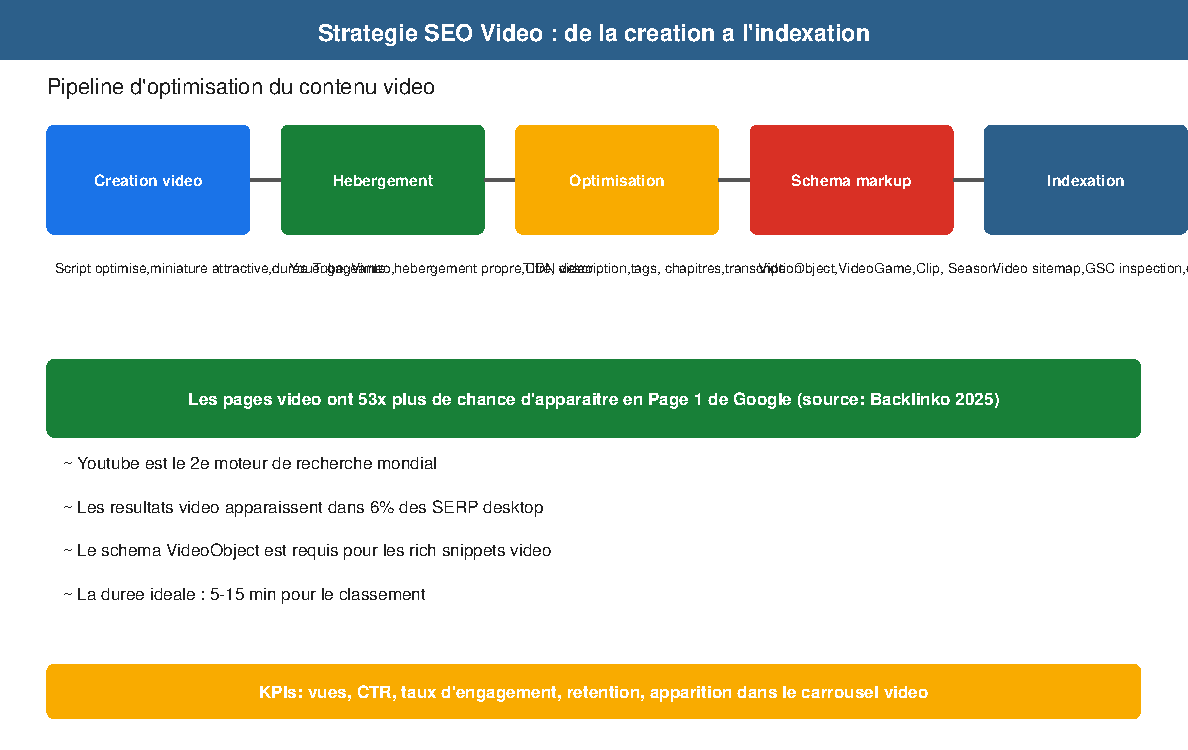
\includegraphics[width=\textwidth]{images/video_seo.pdf}
    \caption{Stratégie SEO Vidéo : de la création à l'indexation}
    \label{fig:video_seo}
\end{figure}

\section{Pourquoi le SEO vidéo est stratégique}

La vidéo représente aujourd'hui plus de 82\% du trafic internet. YouTube est le deuxième moteur de recherche mondial et Google intègre de plus en plus de résultats vidéo dans ses SERP. L'optimisation du \keyword{SEO vidéo} est devenue incontournable pour toute stratégie de contenu.

\subsection{YouTube SEO : facteurs de classement}

YouTube utilise son propre algorithme de classement qui prend en compte plusieurs signaux :

\begin{enumerate}
    \item \textbf{Titre} : Incluez le mot-clé principal au début, idéalement dans les 60 premiers caractères
    \item \textbf{Description} : 200-300 mots, mot-clé dans les premiers 150 caractères, liens utiles
    \item \textbf{Tags} : Mots-clés pertinents, y compris les variantes et synonymes
    \item \textbf{Chapitres vidéo} : Améliorent l'expérience utilisateur et les apparitions dans les featured snippets
    \item \textbf{Transcription et sous-titres} : Texte complet pour l'indexation du contenu parlé
    \item \textbf{Thumbnail personnalisée} : Image de haute qualité avec texte et contraste élevé
    \item \textbf{Engagement} : Temps de visionnage, likes, commentaires, partages
    \item \textbf{Méta-données} : Catégorie, playlist, carte de fin
\end{enumerate}

\begin{mybox}{Facteurs de classement YouTube prioritaires}{googlered}
\begin{itemize}
    \item Temps de visionnage (watch time) et rétention audience
    \item Taux de clic (CTR) depuis les suggestions et les recherches
    \item Pertinence du titre et des tags par rapport à la requête
    \item Engagement post-visionnage (likes, commentaires, abonnements)
    \item Fraîcheur du contenu (date de publication récente)
\end{itemize}
\end{mybox}

\subsection{Optimisation des thumbnails}

La miniature est le premier élément visuel perçu par l'utilisateur. Une thumbnail optimisée peut augmenter le CTR de 30 \% à 50 \%.

\begin{enumerate}
    \item Utilisez des images 1280 × 720 pixels (ratio 16:9)
    \item Ajoutez un texte court et lisible (3-5 mots maximum)
    \item Utilisez des couleurs vives et un contraste élevé
    \item Incluez un visage humain (expression forte)
    \item Testez A/B différentes thumbnails via YouTube Studio
\end{enumerate}

\subsection{Données structurées VideoObject}

Le balisage \keyword{VideoObject} permet à Google d'afficher des rich snippets vidéo dans les résultats de recherche, incluant la durée, la vignette et la date de publication.

\begin{lstlisting}[style=htmlcode,caption={Schema VideoObject au format JSON-LD}]
{
  "@context": "https://schema.org",
  "@type": "VideoObject",
  "name": "Tutoriel SEO : Optimiser ses videos pour Google",
  "description": "Guide complet d'optimisation video SEO...",
  "thumbnailUrl": "https://example.com/thumbnail.jpg",
  "uploadDate": "2026-03-15",
  "duration": "PT15M30S",
  "contentUrl": "https://example.com/video.mp4",
  "embedUrl": "https://youtube.com/embed/xxxxxx",
  "interactionStatistic": {
    "@type": "InteractionCounter",
    "interactionType": "WatchAction",
    "userInteractionCount": 12345
  }
}
\end{lstlisting}

\subsection{Création et soumission d'un sitemap vidéo}

Un \keyword{video sitemap} permet d'indexer spécifiquement les contenus vidéo sur Google.

\begin{lstlisting}[style=htmlcode,caption={Extrait de sitemap vidéo XML}]
<?xml version="1.0" encoding="UTF-8"?>
<urlset xmlns="http://www.sitemaps.org/schemas/sitemap/0.9"
        xmlns:video="http://www.google.com/schemas/sitemap-video/1.1">
  <url>
    <loc>https://example.com/page-video.html</loc>
    <video:video>
      <video:thumbnail_loc>https://example.com/thumb.jpg</video:thumbnail_loc>
      <video:title>Titre de la video</video:title>
      <video:description>Description de la video</video:description>
      <video:content_loc>https://example.com/video.mp4</video:content_loc>
      <video:duration>930</video:duration>
      <video:publication_date>2026-03-15</video:publication_date>
    </video:video>
  </url>
</urlset>
\end{lstlisting}

\subsection{Optimisation du carrousel vidéo Google}

Google affiche souvent un carrousel vidéo pour certaines requêtes. Pour y apparaître :
\begin{itemize}
    \item Utilisez le VideoObject schema sur chaque page de vidéo
    \item Hébergez la vidéo sur une page dédiée (pas de page gallery)
    \item Assurez-vous que la page est indexée et bien optimisée
    \item Utilisez des URLs stables et canoniques
\end{itemize}

\subsection{Hébergement et CDN vidéo}

Le choix de la plateforme d'hébergement impacte le SEO :
\begin{itemize}
    \item \textbf{YouTube} : Idéal pour la découvrabilité, mais pas de contrôle sur les publicités
    \item \textbf{Vimeo} : Meilleure qualité, pas de publicités, mais moins de trafic organique
    \item \textbf{Hébergement propre} : Contrôle total, mais nécessite un CDN performant
    \item \textbf{Wistia / Brightcove} : Solutions professionnelles avec analytics avancés
\end{itemize}

\subsection{SEO pour les podcasts}

Les podcasts audio doivent également être optimisés pour les moteurs de recherche :
\begin{itemize}
    \item Créez une page de destination pour chaque épisode avec un titre et une description uniques
    \item Fournissez une transcription complète (texte) pour l'indexation du contenu parlé
    \item Utilisez le balisage PodcastEpisode et PodcastSeries schema
    \item Soumettez votre flux RSS à Google Podcasts, Apple Podcasts, Spotify
    \item Optimisez le titre et la description de chaque épisode avec les mots-clés cibles
\end{itemize}

\subsection{Cas pratique : Optimisation d'une chaîne e-commerce}

Un site e-commerce d'équipement sportif a optimisé ses 150 vidéos tutoriels avec :
\begin{itemize}
    \item Titres incluant le nom du produit et le mot-clé principal
    \item Descriptions détaillées de 200 mots avec liens vers les fiches produits
    \item Thumbnails personnalisées montrant le produit en action
    \item Chapitres vidéo pour chaque étape du tutoriel
    \item VideoObject schema sur chaque page de vidéo
\end{itemize}
\textbf{Résultat} : +120 \% de trafic organique vers les vidéos, +35 \% de temps passé sur le site, et apparition dans 12 carrousels vidéo Google.

\begin{takeaways}
\begin{itemize}
    \item YouTube est le deuxième moteur de recherche mondial
    \item Le VideoObject schema est indispensable pour les rich snippets vidéo
    \item Les thumbnails personnalisées augmentent significativement le CTR
    \item Les transcriptions améliorent l'indexation du contenu parlé
    \item Un sitemap vidéo accélère la découverte des contenus par Google
\end{itemize}
\end{takeaways}

\level{2}
\begin{objectives}
\begin{itemize}
    \item Comprendre l'essor de la recherche vocale
    \item Adapter le contenu aux requêtes vocales
    \item Implémenter les featured snippets pour le voice search
\end{itemize}
\end{objectives}

\chapter{Le SEO Vocal (Voice Search)}
\label{ch:voice}

\begin{figure}[H]
    \centering
    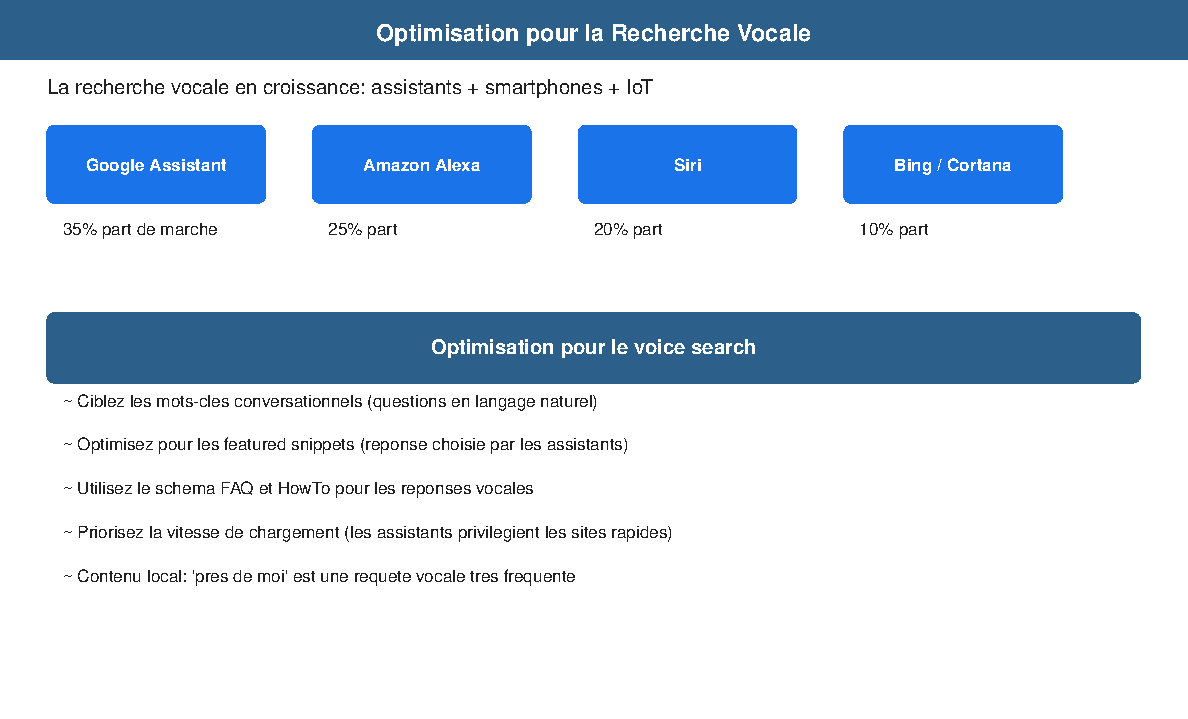
\includegraphics[width=\textwidth]{images/voice_search.pdf}
    \caption{Optimisation pour la recherche vocale : assistants, mots-clés conversationnels et featured snippets}
    \label{fig:voice_search}
\end{figure}

\section{L'essor de la recherche vocale}

Avec l'adoption massive des assistants vocaux (Google Assistant, Siri, Alexa), la \keyword{recherche vocale} transforme la façon dont les utilisateurs interagissent avec les moteurs de recherche. En 2026, plus de 40 \% des adultes utilisent la recherche vocale quotidiennement, et 58 \% des consommateurs l'utilisent pour trouver des informations sur les entreprises locales.

\subsection{Statistiques clés du voice search}

\begin{itemize}
    \item 27 \% de la population mondiale utilise la recherche vocale sur mobile
    \item Le marché des assistants vocaux devrait atteindre 30 milliards de dollars
    \item 72 \% des utilisateurs d'enceintes connectées les utilisent quotidiennement
    \item Les recherches vocales sont 3 fois plus susceptibles d'être locales
    \item La précision de la reconnaissance vocale dépasse 95 \%
\end{itemize}

\subsection{Caractéristiques des requêtes vocales}

\begin{itemize}
    \item \textbf{Requêtes plus longues} : Phrases complètes, questions naturelles (5-10 mots)
    \item \textbf{Intention claire} : Actions spécifiques (acheter, réserver, trouver, appeler)
    \item \textbf{Format question} : "Où trouver...", "Comment faire...", "Quel est le meilleur..."
    \item \textbf{Local} : 58 \% des recherches vocales concernent des entreprises locales
    \item \textbf{Conversationnel} : Langage naturel, pas de mots-clés artificiels
\end{itemize}

\subsection{Différences entre assistants vocaux}

Chaque assistant possède ses spécificités :

\begin{itemize}
    \item \textbf{Google Assistant} : S'appuie sur l'index Google et les featured snippets. Idéal pour le SEO.
    \item \textbf{Apple Siri} : Utilise Google Search et Bing, mais aussi des partenariats spécifiques (Yelp pour le local).
    \item \textbf{Amazon Alexa} : Priorise les réponses depuis ses propres skills et Bing. Moins dépendant du SEO traditionnel.
\end{itemize}

\subsection{Optimisation pour la position zéro (featured snippets)}

Les featured snippets sont la source principale des réponses vocales de Google Assistant :

\begin{enumerate}
    \item Structurez votre contenu en format question-réponse
    \item Utilisez des paragraphes concis de 40-50 mots pour les réponses
    \item Placez la réponse directement après la question (H2 ou H3)
    \item Utilisez des listes à puces et des tableaux pour les réponses structurées
    \item Ciblez les mots-clés en format question (qui, quoi, où, quand, comment, pourquoi)
\end{enumerate}

\subsection{Schémas de données structurées pour la recherche vocale}

Le balisage schema.org permet aux assistants vocaux d'extraire et de formater les réponses :

\begin{lstlisting}[style=htmlcode,caption={FAQPage schema pour les questions fréquentes}]
{
  "@context": "https://schema.org",
  "@type": "FAQPage",
  "mainEntity": [{
    "@type": "Question",
    "name": "Comment optimiser un site pour la recherche vocale ?",
    "acceptedAnswer": {
      "@type": "Answer",
      "text": "Optimisez pour les featured snippets en structurant votre contenu en format question-reponse avec des reponses concises de 40 a 50 mots."
    }
  }]
}
\end{lstlisting}

\begin{mybox}{Speakable schema pour Google Assistant}{googleblue}
Le \keyword{Speakable} schema permet d'indiquer à Google Assistant quelles parties de votre contenu peuvent être lues à voix haute. Il est pris en charge par Google News et les articles de blog.

\begin{lstlisting}[style=htmlcode]
{
  "@context": "https://schema.org",
  "@type": "Article",
  "speakable": {
    "@type": "SpeakableSpecification",
    "cssSelector": [".headline", ".summary"]
  }
}
\end{lstlisting}
\end{mybox}

\subsection{HowTo schema pour les instructions vocales}

Le \keyword{HowTo} schema est particulièrement adapté aux requêtes vocales de type "Comment faire..." :

\begin{lstlisting}[style=htmlcode,caption={HowTo schema pour tutoriels vocaux}]
{
  "@context": "https://schema.org",
  "@type": "HowTo",
  "name": "Comment installer un theme WordPress",
  "step": [{
    "@type": "HowToStep",
    "position": 1,
    "name": "Telecharger le theme",
    "text": "Rendez-vous dans le panneau d'administration WordPress..."
  }]
}
\end{lstlisting}

\subsection{SEO local et recherche vocale}

La recherche vocale est fortement orientée vers le local :

\begin{itemize}
    \item Optimisez votre fiche Google Business Profile (GBP)
    \item Utilisez le LocalBusiness schema pour les données d'entreprise
    \item Incluez des informations de contact (téléphone, adresse, horaires)
    \item Encouragez les avis clients (facteur de classement local important)
    \item Créez du contenu sur des requêtes locales : "près de moi", "à [ville]"
\end{itemize}

\subsection{Page speed et performance mobile}

La vitesse de chargement est critique pour la recherche vocale :

\begin{itemize}
    \item Les utilisateurs vocaux s'attendent à des réponses instantanées
    \item Visez un LCP inférieur à 1,5 seconde (recommandation Google renforcée)
    \item Optimisez les Core Web Vitals (LCP, INP, CLS)
    \item Utilisez l'AMP pour les pages d'articles d'actualité
    \item Mobile-first obligatoire : 90 \% des recherches vocales se font sur mobile
\end{itemize}

\subsection{Cas pratique : Site de recettes optimisé pour le voice search}

Un site de recettes culinaires a optimisé son contenu pour la recherche vocale :

\begin{itemize}
    \item Ajout de FAQ schema sur chaque fiche recette
    \item Reformulation des titres en questions ("Comment faire une pizza maison ?")
    \item Réponses concises de 40 mots directement après chaque question
    \item HowTo schema avec étapes numérotées
    \item Optimisation GBP avec horaires et photos
\end{itemize}
\textbf{Résultat} : Apparition dans 45 featured snippets vocaux, +67 \% de trafic organique, et intégration complète avec Google Assistant pour les requêtes culinaires.

\begin{takeaways}
\begin{itemize}
    \item La recherche vocale privilégie les réponses concises et directes
    \item Les featured snippets sont la source principale des réponses des assistants
    \item Le langage naturel et les questions long-tail sont la clé du SEO vocal
    \item Les schémas FAQ, HowTo et Speakable améliorent la compatibilité vocale
    \item La vitesse de chargement est un facteur critique pour l'expérience vocale
\end{itemize}
\end{takeaways}

\level{3}
\begin{objectives}
\begin{itemize}
    \item Comprendre les fondamentaux du SEO split testing
    \item Maîtriser la méthodologie de test A/B
    \item Savoir interpréter la signification statistique des tests
\end{itemize}
\end{objectives}

\chapter{A/B Testing et Expérimentation SEO}
\label{ch:seotesting}

\begin{figure}[H]
    \centering
    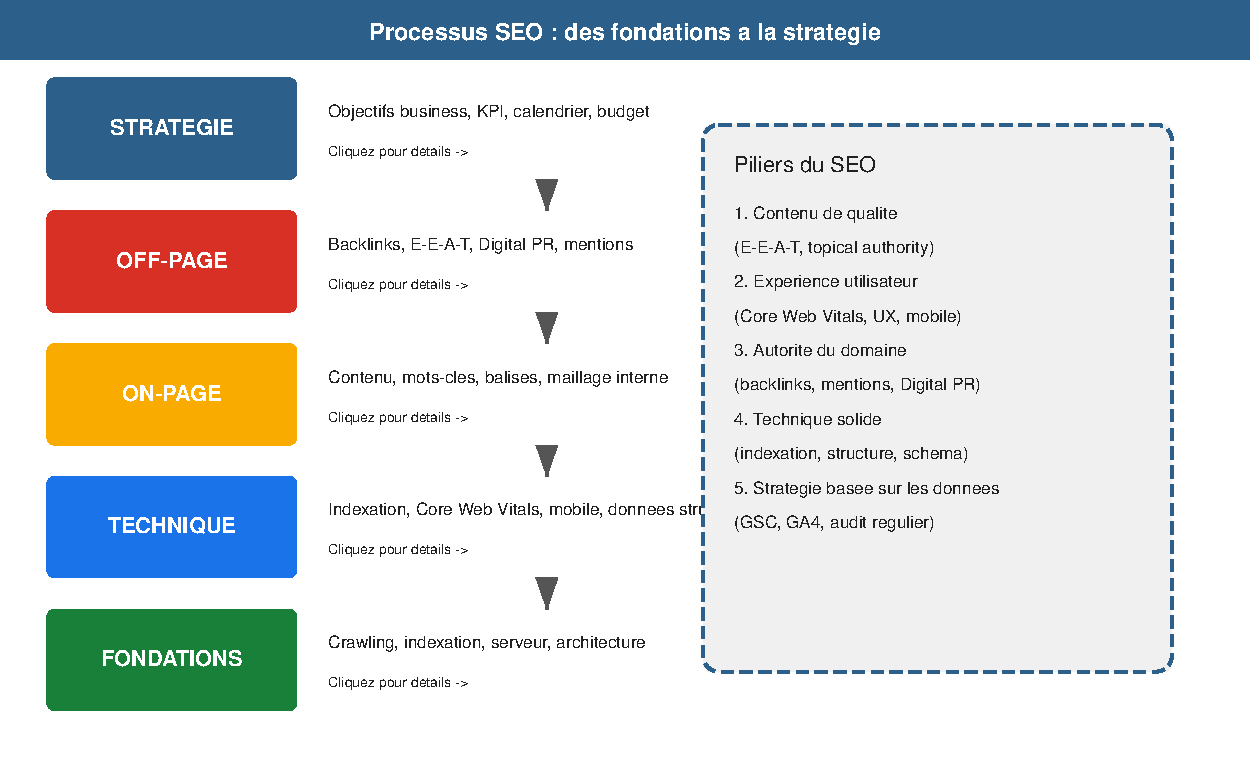
\includegraphics[width=\textwidth]{images/seo_process_overview.pdf}
    \caption{Méthodologie d'expérimentation SEO : tester, mesurer, itérer}
    \label{fig:abtesting_process}
\end{figure}

\section{Fondamentaux du SEO Split Testing}

Le \keyword{SEO split testing} (ou A/B testing SEO) consiste a tester des modifications sur des pages web pour mesurer leur impact sur le trafic organique et les positions.

\subsection{Pourquoi tester en SEO ?}

\begin{itemize}
    \item \textbf{Valider les hypotheses} : Remplacer l'intuition par des données
    \item \textbf{Eviter les erreurs couteuses} : Un mauvais changement peut faire perdre des mois de trafic
    \item \textbf{Comprendre l'algorithme} : Decouvrir ce que Google valorise réellement
    \item \textbf{Optimiser le ROI} : Investir uniquement dans les changements qui fonctionnent
\end{itemize}

\section{Méthodologie de test}

\subsection{Types de tests SEO}

\begin{itemize}
    \item \textbf{A/B test (split test)} : Deux versions d'une meme page, reparties sur des URLs similaires
    \item \textbf{Before/After} : Mesure avant et après un changement (moins fiable)
    \item \textbf{Test apparie} : Comparaison de pages de catégories similaires
    \item \textbf{Test temps réel} : Monitoring continu avec ajustements dynamiques
\end{itemize}

\subsection{Processus de test rigoureux}

\begin{enumerate}
    \item \textbf{Hypothese} : Formulez clairement ce que vous testez et pourquoi
    \item \textbf{Selection de l'echantillon} : Pages suffisamment nombreuses et similaires
    \item \textbf{Duree du test} : Minimum 2--4 semaines (cycles de crawl Google)
    \item \textbf{Mesure} : Positions, trafic, CTR, imprèssions, conversions
    \item \textbf{Analyse} : Signification statistique avant conclusion
    \item \textbf{Deploiement} : Appliquer la version gagnante
    \item \textbf{Validation} : Confirmer les résultats sur la duree
\end{enumerate}

\section{Signification statistique en SEO}

La \keyword{signification statistique} est cruciale pour ne pas tirer de conclusions hatives :

\begin{itemize}
    \item \textbf{Niveau de confiance} : 95\% minimum (p-value $<$ 0.05)
    \item \textbf{Taille d'echantillon} : Plus le trafic est faible, plus le test doit etre long
    \item \textbf{PageRank et autorite} : Des pages comparables en termes d'autorite
    \item \textbf{Saisonnalite} : Tester sur des périodes similaires
    \item \textbf{Bruit algorithmique} : Les fluctuations normales des SERP peuvent masquer les effets
\end{itemize}

\begin{mybox}{Calculateur de signification}{googleblue}
Pour determiner si un résultat est statistiquement significatif :
\[
z = \frac{\text{CTR}_{\text{test}} - \text{CTR}_{\text{contrôle}}}
{\sqrt{\frac{\text{CTR}_{\text{contrôle}}(1 - \text{CTR}_{\text{contrôle}})}{n}}}
\]
Ou $n$ est le nombre d'imprèssions. Un $z > 1.96$ indique une signification a 95\%.
\end{mybox}

\section{Outils de SEO Testing}

\subsection{Outils spécialisés}

\begin{itemize}
    \item \textbf{SearchPilot} : Outil professionnel de A/B testing SEO
    \item \textbf{AB Tasty} : CRO + testing SEO avec intégration GA4
    \item \textbf{VWO (Visual Website Optimizer)} : Testing avec segmentation par source de trafic
    \item \textbf{Dynamic Yield} : Personalisation et testing SEO
    \item \textbf{Google Analytics 4} : Experiences A/B natives dans GA4
    \item \textbf{Cloudflare A/B Testing} : Testing au niveau CDN
\end{itemize}

\section{Elements a tester en priorité}

\subsection{Title Tags}

Les \keyword{title tags} sont l'élément le plus teste en SEO :

\begin{itemize}
    \item \textbf{Format} : "Mot-cle principal -- Secondaire | Marque" vs "Marque | Mot-cle principal"
    \item \textbf{Longueur} : 50--60 caracteres vs plus long
    \item \textbf{Number} : Titrès avec chiffres vs sans
    \item \textbf{Emotion} : Mots puissants vs neutrès
    \item \textbf{Question} : Titrès interrogatifs vs affirmatifs
    \item \textbf{Annee} : Inclure l'annee en cours vs ne pas l'inclure
\end{itemize}

\subsection{Meta Descriptions}

\begin{itemize}
    \item \textbf{Longueur} : 155--160 caracteres vs plus court
    \item \textbf{CTA} : "Decouvrez" vs "Achetez" vs "Apprenez"
    \item \textbf{Inclusion de mots-clés} : En debut vs répartis
    \item \textbf{Structure} : Liste vs paragraphe
    \item \textbf{Questions} : Description sous forme de question vs affirmation
\end{itemize}

\subsection{Contenu et structure}

\begin{itemize}
    \item \textbf{Longueur du contenu} : 1500 mots vs 3000 mots
    \item \textbf{Format} : Listes vs paragraphes vs guides
    \item \textbf{H1} : Avec mot-cle exact vs variante sémantique
    \item \textbf{Sous-titrès} : H2/H3 structures vs contenu non structure
    \item \textbf{Images} : Avec images vs sans, position des images
    \item \textbf{CTA} : Position (haut vs bas), formulation
\end{itemize}

\subsection{Données structureées}

\begin{itemize}
    \item FAQ schema vs pas de FAQ
    \item HowTo schema pour les tutoriels
    \item Review schema (etoiles) vs pas d'avis structures
    \item Article schema enrichi vs basique
\end{itemize}

\begin{lstlisting}[style=code,caption={Exemple de test A/B sur les title tags (Python)}]
import numpy as np
from scipy import stats

def test_title_tag(control_data, variant_data):
    imprèssions_c, clics_c = control_data
    imprèssions_v, clics_v = variant_data

    ctr_c = clics_c / imprèssions_c
    ctr_v = clics_v / imprèssions_v

    # Test de proportion (z-test)
    p_pool = (clics_c + clics_v) / (imprèssions_c + imprèssions_v)
    se = np.sqrt(p_pool * (1 - p_pool) * (1/imprèssions_c + 1/imprèssions_v))
    z = (ctr_v - ctr_c) / se
    p_value = 2 * (1 - stats.norm.cdf(abs(z)))

    uplift = (ctr_v - ctr_c) / ctr_c * 100

    return {
        "ctrl_ctr": round(ctr_c * 100, 2),
        "variant_ctr": round(ctr_v * 100, 2),
        "uplift": round(uplift, 2),
        "z_score": round(z, 3),
        "p_value": round(p_value, 4),
        "significant": p_value < 0.05
    }

# Exemple : Test de title avec "2026" vs sans
résultat = test_title_tag(
    control_data=[50000, 2500],
    variant_data=[48000, 2640]
)
print(résultat)
# Sortie : {'ctrl_ctr': 5.0, 'variant_ctr': 5.5,
#           'uplift': 10.0, 'z_score': 3.556,
#           'p_value': 0.0004, 'significant': True}
\end{lstlisting}

\section{Eviter les pieges SEO dans les tests}

\begin{mybox}{Pieges courants du SEO Testing}{googlered}
\begin{itemize}
    \item \textbf{Contenu duplique} : Les deux versions d'un test ne doivent pas etre indexees
    \item \textbf{Canonical incorrect} : Utiliser une balise canonical sur la version de contrôle
    \item \textbf{Noindex accidentel} : Ne pas noindex la variante
    \item \textbf{Delai insuffisant} : Google peut mettre 2 a 4 semaines a recrawler une page
    \item \textbf{Echantillon trop petit} : Moins de 1000 imprèssions par variante = données non significatives
    \item \textbf{Tester plusieurs changements} : Impossible d'isolér la cause
    \item \textbf{Saisonnalite non prise en compte} : Comparer fevrier avec decembre = biais
\end{itemize}
\end{mybox}

\subsection{Methode recommandée : Split par URLs}

\begin{enumerate}
    \item Identifiez un groupe de pages similaires (ex: 100 fiches produits)
    \item Divisez aleatoirement en groupe contrôle (50) et groupe test (50)
    \item Appliquez la modification sur le groupe test uniquement
    \item Comparez les performances des deux groupes sur 4 semaines
    \item Assurez-vous que les groupes sont statistiquement équivalents en pré-test
\end{enumerate}

\section{Cas pratiques de SEO Testing}

\subsection{Cas 1 : Test de longueur de contenu}

\textbf{Hypothese :} Les articles de plus de 2000 mots génèrent 50\% plus de trafic que les articles de 1000 mots.

\textbf{Resultat :} +67\% de trafic pour le groupe B, +42\% de backlinks. Significatif a 99\%.

\subsection{Cas 2 : Test de title tags avec numero}

\textbf{Hypothese :} Les titrès commencant par un chiffre (ex: "10 facons de...") génèrent plus de clics.

\textbf{Resultat :} +23\% de CTR pour les titrès numerotes a position egale.

\subsection{Cas 3 : Test de FAQ Schema}

\textbf{Hypothese :} L'ajout de FAQ schema améliore la visibilité dans les featured snippets.

\textbf{Resultat :} +15\% de featured snippets, +8\% de trafic.

% =============================================================================

% ============================================
% PARTIE 7 : MESURE ET ANALYSE
% ============================================

\part{La Mesure et l'Analyse}
\label{part:mesure}

% ========== CHAPITRE 25 ==========
\begin{takeaways}
\begin{itemize}
    \item Les tests SEO doivent respecter des contraintes spécifiques
    \item La signification statistique est essentielle pour valider les résultats
    \item Les title tags et les données structurées sont prioritaires à tester
\end{itemize}
\end{takeaways}

\level{1}
\begin{objectives}
\begin{itemize}
    \item Savoir utiliser Google Search Console
    \item Maîtriser les rapports essentiels
    \item Diagnostiquer les problèmes via GSC
\end{itemize}
\end{objectives}

\chapter{Google Search Console}
\label{ch:gsc}

\begin{figure}[H]
    \centering
    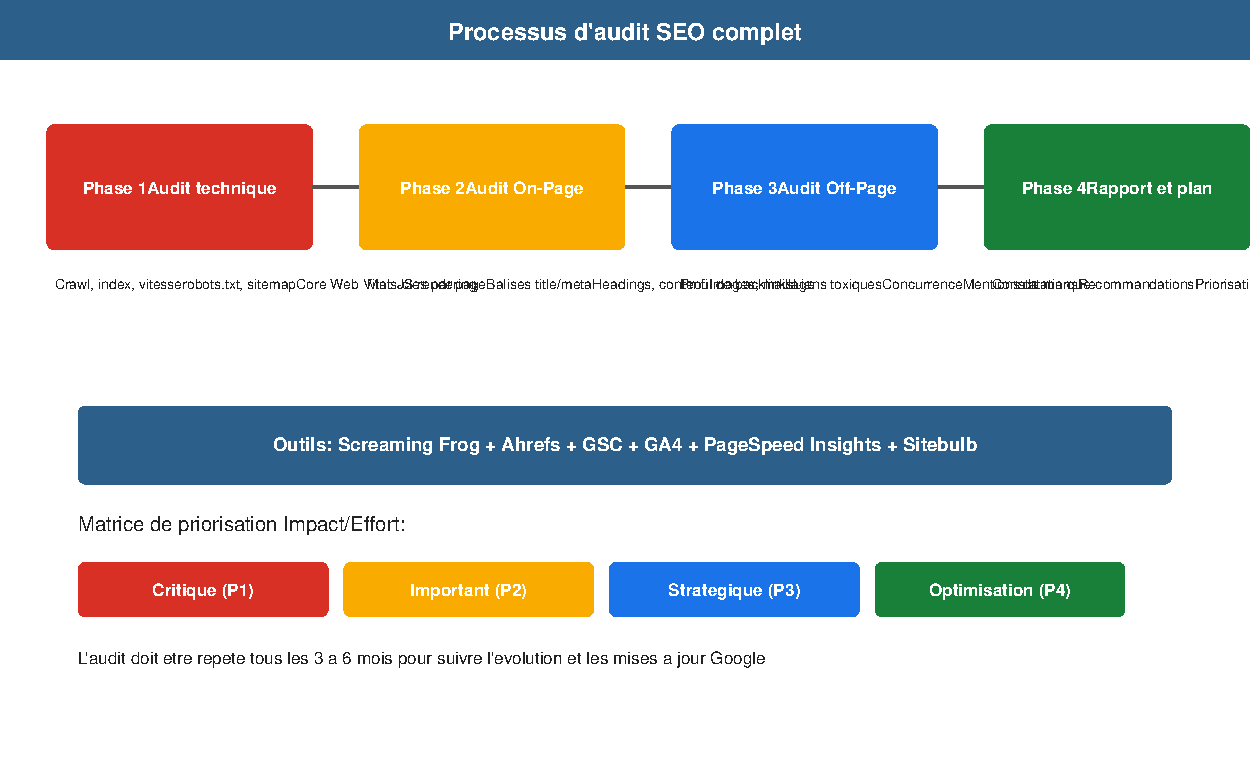
\includegraphics[width=\textwidth]{images/audit_process.pdf}
    \caption{Processus complet d'audit SEO en quatre phases : technique, on-page, off-page et rapport}
    \label{fig:audit_process}
\end{figure}

\section{Présentation de Google Search Console}

Le \keyword{Google Search Console} (GSC) est l'outil gratuit le plus important pour tout professionnel du SEO. Il fournit des données directes de l'index Google sur votre site. Sans GSC, aucune stratégie SEO ne peut être complète, car il s'agit de la source la plus fiable pour comprendre comment Google perçoit votre site.

\subsection{Configuration et vérification de propriété}

Pour utiliser GSC, vous devez d'abord vérifier que vous êtes propriétaire du site :
\begin{itemize}
    \item \textbf{Fichier HTML} : Téléchargez un fichier de vérification à la racine du site
    \item \textbf{Balise meta} : Ajoutez une balise dans le \texttt{<head>} de la page d'accueil
    \item \textbf{Google Analytics} : Utilisez votre compte GA4 existant
    \item \textbf{Google Tag Manager} : Via le conteneur GTM
    \item \textbf{DNS} : Ajoutez un enregistrement TXT dans votre zone DNS
\end{itemize}

\subsection{Le rapport Performance}

Le rapport Performance est le cœur de GSC :

\begin{mybox}{Métriques clés du rapport Performance}{googleblue}
\begin{itemize}
    \item \textbf{Clics} : Nombre total de clics depuis les SERP vers votre site
    \item \textbf{Impressions} : Nombre de fois où votre site est apparu dans les SERP
    \item \textbf{CTR} : Taux de clic (clics / impressions)
    \item \textbf{Position moyenne} : Position moyenne de vos pages dans les SERP
\end{itemize}
\end{mybox}

\begin{itemize}
    \item Filtrer par requête, page, pays, appareil, type de recherche (web, image, vidéo)
    \item Comparer les périodes (28 jours, 7 jours, personnalisé)
    \item Analyser les tendances : baisse soudaine du trafic, pics saisonniers
    \item Exporter les données vers Google Sheets ou CSV via l'API
\end{itemize}

\subsubsection{Analyse des tendances dans le rapport Performance}

Pour exploiter pleinement le rapport Performance :
\begin{enumerate}
    \item Identifiez les requêtes en hausse et en baisse significative
    \item Analysez les requêtes à fort CTR mais faible position (opportunités d'optimisation)
    \item Repérez les pages qui perdent des impressions (problème technique potentiel)
    \item Comparez les performances mobiles vs desktop
    \item Segmentez par pays pour le SEO international
\end{enumerate}

\subsection{Le rapport Indexation (Couverture)}

Le rapport de couverture indique l'état d'indexation de chaque page :

\begin{itemize}
    \item \textbf{Erreur} : Page non indexée (404, 500, blocage par robots.txt, etc.)
    \item \textbf{Avertissement} : Page indexée avec problèmes (canonical incorrect, page sans contenu)
    \item \textbf{Valide} : Page indexée correctement et sans erreur
    \item \textbf{Exclue} : Page non indexée délibérément (noindex, redirection, page non canonique)
\end{itemize}

\begin{mybox}{Erreurs d'indexation courantes et solutions}{googlered}
\begin{itemize}
    \item \textbf{404 (Not found)} : Rediriger vers une page pertinente avec une redirection 301
    \item \textbf{Soft 404} : Corriger la page ou ajouter du contenu substantiel
    \item \textbf{Blocage par robots.txt} : Modifier robots.txt pour autoriser le crawl
    \item \textbf{Redirection en chaîne} : Réduire le nombre de redirections consécutives
    \item \textbf{Timeout serveur} : Améliorer le temps de réponse du serveur
\end{itemize}
\end{mybox}

\subsection{L'outil d'inspection d'URL}

L'inspection d'URL permet de diagnostiquer précisément l'indexation d'une page :

\begin{enumerate}
    \item Entrez une URL spécifique dans la barre de recherche GSC
    \item Consultez le statut d'indexation : indexée ou non, avec la date du dernier crawl
    \item Vérifiez la date du dernier crawl et la version de la page analysée
    \item Visualisez la page rendue par Google (rendu Googlebot)
    \item Testez l'URL en direct pour voir sa version actuelle
    \item Demandez une indexation manuelle après avoir corrigé un problème
\end{enumerate}

\subsection{Core Web Vitals}

Le rapport Core Web Vitals regroupe les métriques de performance :

\begin{itemize}
    \item \textbf{LCP (Largest Contentful Paint)} : Temps de chargement du contenu principal (< 2,5 s)
    \item \textbf{INP (Interaction to Next Paint)} : Réactivité aux interactions (< 200 ms)
    \item \textbf{CLS (Cumulative Layout Shift)} : Stabilité visuelle (< 0,1)
\end{itemize}
Le rapport GSC classe les URLs en trois catégories : Bon, À améliorer, Mauvais. Utilisez ces données pour prioriser les corrections techniques sur les pages ayant le plus fort impact.

\subsection{Gestion des sitemaps}

La section Sitemaps de GSC permet de soumettre et de monitorer vos sitemaps XML :

\begin{enumerate}
    \item Soumettez l'URL complète du sitemap via l'interface
    \item Vérifiez le nombre d'URLs découvertes vs le nombre d'URLs soumises
    \item Surveillez les erreurs de sitemap (format invalide, URLs bloquées)
    \item Consultez la date du dernier crawl de chaque sitemap
    \item Supprimez les sitemaps obsolètes après une migration de site
\end{enumerate}

\subsection{Liens internes et externes}

Le rapport Liens fournit des informations précieuses :
\begin{itemize}
    \item \textbf{Liens externes} : Domaines référents, liens les plus fréquents, texte d'ancrage
    \item \textbf{Liens internes} : Pages les plus liées en interne, répartition du maillage
\end{itemize}
Ces données sont essentielles pour analyser votre profil de backlinks et optimiser votre maillage interne.

\subsection{GSC API pour l'automatisation du reporting}

L'API GSC permet d'exporter les données vers des outils externes :

\begin{lstlisting}[style=htmlcode,caption={Script Python pour exporter les données GSC}]
from google.oauth2 import service_account
from googleapiclient.discovery import build

SCOPES = ['https://www.googleapis.com/auth/webmasters.readonly']
SERVICE_ACCOUNT_FILE = 'gsc-credentials.json'

credentials = service_account.Credentials.from_service_account_file(
    SERVICE_ACCOUNT_FILE, scopes=SCOPES)
service = build('searchconsole', 'v1', credentials=credentials)

site_url = 'sc-domain:monsite.com'
request = {
    'startDate': '2026-01-01',
    'endDate': '2026-03-31',
    'dimensions': ['query', 'page'],
    'rowLimit': 1000
}
response = service.searchanalytics().query(
    siteUrl=site_url, body=request).execute()
for row in response.get('rows', []):
    print(f"{row['keys'][0]} | {row['keys'][1]} | "
          f"Clics: {row['clicks']} | Impressions: {row['impressions']} | "
          f"CTR: {row['ctr']:.2%} | Position: {row['position']:.1f}")
\end{lstlisting}

\subsection{Cas pratique : Diagnostic SEO via GSC}

Un magazine en ligne a perdu 40 \% de son trafic organique. L'analyse GSC a révélé :
\begin{itemize}
    \item 15 000 erreurs 410 (pages supprimées sans redirection)
    \item 8 000 pages bloquées par un robots.txt mal configuré après migration
    \item 3 000 URLs soft 404 (pages devenues vides après refonte)
    \item Chute de 60 \% des impressions pour les articles de plus de 2 ans
\end{itemize}
\textbf{Corrections} : Redirections 301 pour les pages supprimées, correction du robots.txt, suppression des pages vides, ajout de contenu frais aux articles anciens. \\
\textbf{Résultat} : Récupération de 70 \% du trafic en 8 semaines et amélioration du taux d'indexation de 85 \% à 97 \%.

\begin{takeaways}
\begin{itemize}
    \item GSC est l'outil gratuit indispensable pour tout professionnel SEO
    \item Le rapport de couverture identifie précisément les problèmes d'indexation
    \item Le rapport Performance analyse le trafic organique par requête et par page
    \item L'inspection d'URL permet un diagnostic précis de chaque page
    \item L'API GSC facilite l'automatisation du reporting SEO
\end{itemize}
\end{takeaways}

\level{2}
\begin{objectives}
\begin{itemize}
    \item Comprendre les spécificités de GA4 par rapport à Universal Analytics
    \item Identifier les métriques clés pour le SEO dans GA4
    \item Configurer les rapports SEO avancés dans GA4
\end{itemize}
\end{objectives}

\chapter{Google Analytics 4 (GA4)}
\label{ch:ga4}

\section{Comprendre GA4}

\keyword{Google Analytics 4} (GA4) est la dernière version de Google Analytics, basée sur les événements plutôt que sur les sessions. Il remplace Universal Analytics depuis juillet 2023. Contrairement à UA qui utilisait un modèle de données basé sur les sessions et les pageviews, GA4 utilise un modèle entièrement événementiel qui offre plus de flexibilité dans l'analyse du comportement utilisateur.

\subsection{GA4 vs Universal Analytics : différences fondamentales}

\begin{itemize}
    \item \textbf{Modèle de données} : Événements vs Sessions. Tout est un événement (page\_view, scroll, click, conversion)
    \item \textbf{Paramètres} : Jusqu'à 100 paramètres par événement (25 dans UA), avec 50 paramètres de texte
    \item \textbf{Identité utilisateur} : User-ID, Google Signals, device ID (modèle d'identité unifié)
    \item \textbf{Métriques} : Engagement rate remplace le taux de rebond, sessions engagées remplacent les sessions simples
    \item \textbf{Période de conservation} : Jusqu'à 14 mois (contre 26 mois pour UA gratuit)
    \item \textbf{Modélisation} : Modélisation du comportement des cookies (conformité RGPD intégrée)
    \item \textbf{Rapports} : Explorations personnalisées (Analysis Hub) vs rapports prédéfinis uniquement
\end{itemize}

\subsection{Le modèle événementiel de GA4}

Dans GA4, les événements sont classés en plusieurs catégories :
\begin{itemize}
    \item \textbf{Événements collectés automatiquement} : page\_view, session\_start, first\_visit, scroll, click, etc.
    \item \textbf{Événements améliorés} : outbound click, site search, video engagement, file download, etc.
    \item \textbf{Événements personnalisés} : définis par vos soins via gtag.js ou Google Tag Manager
    \item \textbf{Événements recommandés} : définis par Google pour l'e-commerce (purchase, add\_to\_cart, etc.)
\end{itemize}

\subsection{Les rapports clés de GA4 pour le SEO}

\subsubsection{Rapport Acquisition}

Le rapport Acquisition montre comment les utilisateurs arrivent sur votre site :
\begin{itemize}
    \item \textbf{Trafic organique} : Sessions provenant des moteurs de recherche
    \item \textbf{Organic Search} : Segment par moteur (Google, Bing, DuckDuckGo)
    \item \textbf{Landing page} : Pages d'entrée principales pour le trafic organique
    \item \textbf{Source / Medium} : Distinction entre les différentes sources SEO
\end{itemize}

\subsubsection{Rapport Engagement}

Mesure l'interaction des utilisateurs avec votre contenu :
\begin{itemize}
    \item \textbf{Sessions engagées} : Sessions durant plus de 10 secondes, avec conversion ou 2+ pages vues
    \item \textbf{Engagement rate} : Pourcentage de sessions engagées (métrique clé de GA4)
    \item \textbf{Vues par session} : Profondeur de navigation moyenne
    \item \textbf{Temps d'engagement moyen} : Durée réelle d'interaction (plus précis que le temps passé)
    \item \textbf{Pages et écrans} : Performance de chaque page (titre, URL, chemin)
\end{itemize}

\subsection{Connecter GA4 avec Google Search Console}

La liaison GSC-GA4 est essentielle pour l'analyse SEO :

\begin{enumerate}
    \item Dans GA4, allez dans Admin > Product Links > Search Console Links
    \item Sélectionnez votre propriété GSC (site complet ou sous-domaine)
    \item Activez l'export des données GSC dans GA4
    \item Accédez aux rapports Acquisition > Search Console
    \item Consultez les données : requêtes, pages, impressions, clics, CTR, position moyenne
\end{enumerate}

\begin{mybox}{Dimensions SEO disponibles après connexion GSC}{googleblue}
\begin{itemize}
    \item \textbf{Landing page} : URL de la page d'entrée (dimension primaire)
    \item \textbf{Query} : Requête de recherche exacte (mot-clé ayant généré l'impression)
    \item \textbf{Source / Medium} : google / organic pour le trafic naturel
    \item \textbf{Pays} : Localisation géographique de l'utilisateur
    \item \textbf{Appareil} : Mobile, desktop, tablette
\end{itemize}
\end{mybox}

\subsection{Créer des explorations pour l'analyse SEO}

L'Exploration (Analysis Hub) de GA4 permet des analyses personnalisées puissantes :

\begin{itemize}
    \item \textbf{Exploration en entonnoir} : Analyser le parcours de conversion des utilisateurs organiques
    \item \textbf{Exploration de segments} : Comparer le comportement des utilisateurs organiques vs payants
    \item \textbf{Exploration de cohortes} : Analyser la rétention des utilisateurs SEO sur 7, 14, 30 jours
    \item \textbf{Exploration des chemins} : Visualiser les parcours de navigation après arrivée organique
    \item \textbf{Segment d'audience} : Créer un segment "Trafic organique" réutilisable dans tous les rapports
\end{itemize}

\subsection{Configurer les conversions SEO dans GA4}

Pour suivre les objectifs SEO dans GA4 :
\begin{enumerate}
    \item Identifiez les actions clés : soumission de formulaire, inscription newsletter, achat, téléchargement
    \item Créez des événements personnalisés via Google Tag Manager
    \item Marquez ces événements comme conversions dans GA4 (Admin > Conversions)
    \item Utilisez l'exploration pour mesurer le taux de conversion par source
    \item Associez les conversions aux landing pages pour identifier les pages les plus performantes
\end{enumerate}

\subsection{Cas pratique : Analyse SEO via GA4}

Une plateforme e-learning a utilisé GA4 pour améliorer son SEO :
\begin{itemize}
    \item Connexion GSC-GA4 pour obtenir les données de requêtes directement dans GA4
    \item Création d'un segment "Trafic organique engagé" (sessions avec lecture de contenu > 30 secondes)
    \item Analyse des pages à fort trafic mais faible engagement (problème de contenu ou de pertinence)
    \item Identification des 50 landing pages générant le plus d'inscriptions newsletter via le parcours de conversion
    \item Optimisation des pages à fort potentiel mais faible taux de conversion
\end{itemize}
\textbf{Résultat} : +40 \% de conversions issues du trafic organique, identification de 20 pages prioritaires à optimiser, et amélioration de 25 \% du taux d'engagement des sessions organiques.

\begin{takeaways}
\begin{itemize}
    \item GA4 utilise un modèle de données basé sur les événements, plus flexible qu'UA
    \item L'engagement rate remplace le taux de rebond comme métrique d'interaction principale
    \item La connexion GSC-GA4 est indispensable pour l'analyse SEO avancée
    \item Les explorations permettent des analyses personnalisées puissantes
    \item Les segments "trafic organique" facilitent l'analyse comparative des sources
\end{itemize}
\end{takeaways}

\level{2}
\begin{objectives}
\begin{itemize}
    \item Identifier les indicateurs essentiels du SEO
    \item Savoir construire un tableau de bord SEO complet
    \item Maîtriser le reporting SEO automatisé
\end{itemize}
\end{objectives}

\chapter{Les KPIs SEO et le Reporting}
\label{ch:kpis}

\begin{figure}[H]
    \centering
    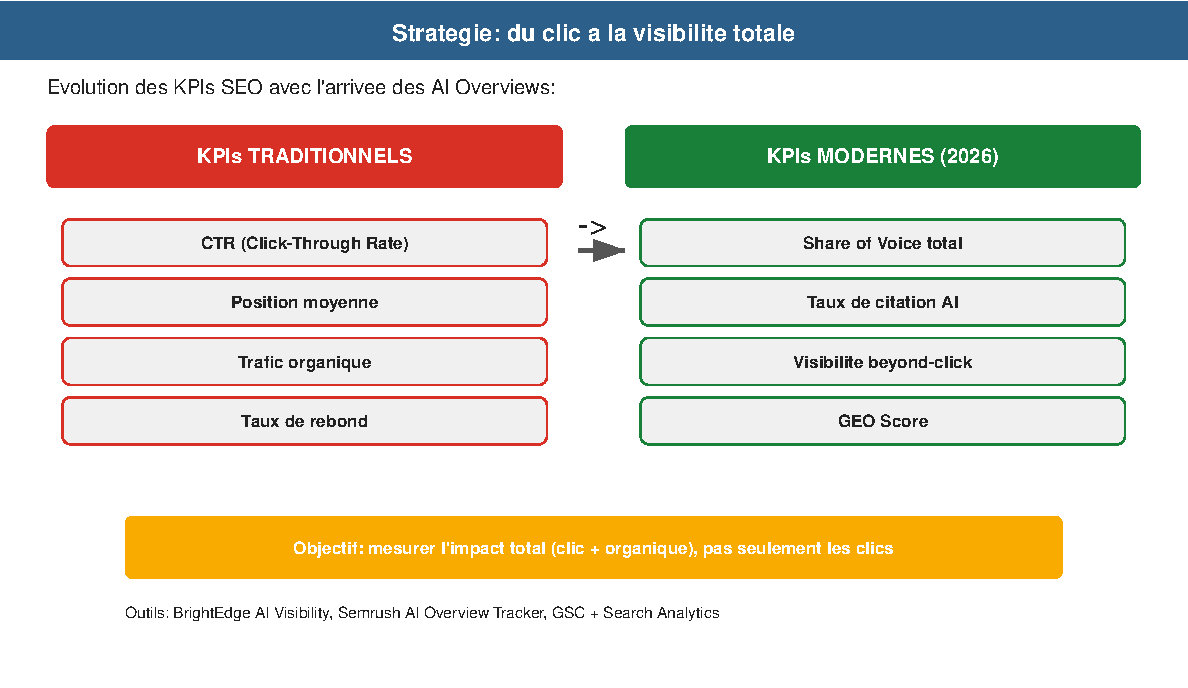
\includegraphics[width=\textwidth]{images/traffic_visibility.pdf}
    \caption{Du CTR à la visibilité totale : l'évolution des KPIs SEO à l'ère des AI Overviews}
    \label{fig:kpi_evolution}
\end{figure}

\section{Les indicateurs essentiels}

Un \keyword{KPI SEO} (Key Performance Indicator) est une métrique mesurable qui évalue l'efficacité d'une stratégie de référencement naturel. Les KPIs SEO se répartissent en plusieurs catégories complémentaires qu'il est essentiel de suivre de manière cohérente pour piloter sa stratégie.

\subsection{Le cadre complet des KPIs SEO}

\subsubsection{Métriques de trafic}

\begin{itemize}
    \item \textbf{Sessions organiques} : Volume de visites provenant des moteurs de recherche
    \item \textbf{Utilisateurs organiques} : Nombre d'utilisateurs uniques (dédoublonnés)
    \item \textbf{Nouveaux utilisateurs} : Proportion de nouveaux visiteurs issus du SEO
    \item \textbf{Pages vues organiques} : Volume total de pages consultées par les visiteurs SEO
    \item \textbf{Sessions par utilisateur} : Fréquence de retour des visiteurs organiques
\end{itemize}

\subsubsection{Métriques techniques}

\begin{itemize}
    \item \textbf{Pourcentage de pages indexées} : Pages indexées / pages totales (idéal > 90 \%)
    \item \textbf{Crawl budget utilisé} : Pages crawllées par Googlebot par jour
    \item \textbf{Core Web Vitals} : LCP (< 2,5 s), INP (< 200 ms), CLS (< 0,1)
    \item \textbf{Taux d'erreurs 4xx / 5xx} : Pourcentage d'erreurs serveur et client
    \item \textbf{Temps de chargement} : Temps moyen de chargement des pages (mobile et desktop)
    \item \textbf{Mobile usability} : Pourcentage de pages sans erreurs d'affichage mobile
\end{itemize}

\subsubsection{Métriques off-page}

\begin{itemize}
    \item \textbf{Nombre de domaines référents} : Nombre de sites uniques qui pointent vers le vôtre
    \item \textbf{Nouveaux backlinks} : Liens entrants acquis sur une période donnée
    \item \textbf{Backlinks perdus} : Liens entrants supprimés ou devenus inaccessibles
    \item \textbf{Qualité des backlinks} : Autorité des domaines référents (DR, TF, CF)
    \item \textbf{Répartition des ancres} : Distribution des textes d'ancrage (exact, branded, générique)
\end{itemize}

\subsubsection{Métriques de conversion}

\begin{itemize}
    \item \textbf{Taux de conversion organique} : Conversions / sessions organiques
    \item \textbf{Objectifs atteints} : Nombre d'objectifs complétés (achats, inscriptions, téléchargements)
    \item \textbf{Revenu organique} : Chiffre d'affaires généré par le trafic SEO
    \item \textbf{Valeur moyenne de commande (AOV)} : Panier moyen des clients issus du SEO
    \item \textbf{Taux de rebond adapté GA4} : Sessions non engagées (durée < 10 secondes, 1 page)
\end{itemize}

\subsection{Tableau de bord SEO structuré}

\begin{table}[H]
\centering
\caption{Indicateurs clés de performance SEO par catégorie}
\label{tab:kpis}
\begin{tabular}{|l|l|}
\hline
\rowcolor{primary}\textcolor{white}{\textbf{Catégorie}} & \textcolor{white}{\textbf{Indicateur}} \\
\hline
Trafic organique & Sessions, utilisateurs, pages vues \\
\hline
Classement & Position moyenne par mot-clé \\
\hline
Taux de conversion & Objectifs atteints / sessions \\
\hline
Autorité & Domain Authority, Trust Flow, Citation Flow \\
\hline
Indexation & Pages indexées, erreurs de crawl \\
\hline
Core Web Vitals & LCP, INP, CLS \\
\hline
Backlinks & Nombre de domaines référents, nouveaux / pertes \\
\hline
CTR & Taux de clic moyen dans les SERP \\
\hline
Engagement & Temps passé, pages par session \\
\hline
\end{tabular}
\end{table}

\subsection{Création d'un dashboard Looker Studio}

Looker Studio (anciennement Google Data Studio) permet de créer des tableaux de bord SEO interactifs :

\begin{enumerate}
    \item Connectez les sources de données : GSC, GA4, Google Sheets, Ahrefs / SEMrush
    \item Créez une page principale avec les métriques globales (trafic, clics, impressions)
    \item Ajoutez une page détaillée avec les tendances par requête et par page
    \item Intégrez des alertes visuelles pour les baisses significatives de trafic
    \item Planifiez un envoi automatique par email (hebdomadaire ou mensuel)
    \item Utilisez les segments temporels pour comparer les périodes (mois vs mois, année vs année)
\end{enumerate}

\subsection{Reporting mensuel et trimestriel}

Le rythme de reporting dépend des destinataires et des objectifs :

\begin{mybox}{Rythme de reporting recommandé}{googleblue}
\begin{itemize}
    \item \textbf{Reporting hebdomadaire (opérationnel)} : Trafic, clics GSC, alertes, problèmes techniques urgents
    \item \textbf{Reporting mensuel (tactique)} : Classements, backlinks, Core Web Vitals, objectifs atteints
    \item \textbf{Reporting trimestriel (stratégique)} : Tendances sur 3 mois, ROI, analyses concurrentielles
    \item \textbf{Reporting annuel (direction)} : Bilan complet, perspectives, budget et ressources
\end{itemize}
\end{mybox}

\subsection{Reporting exécutif vs technique}

Adaptez votre reporting au public cible :
\begin{itemize}
    \item \textbf{Direction / Clients} : Métriques business (trafic, revenu, ROI), tendances macro, recommandations stratégiques
    \item \textbf{Équipe technique} : Core Web Vitals, erreurs d'indexation, problèmes de crawl, données structurées
    \item \textbf{Équipe contenu} : Positions par mot-clé, CTR, pages les plus performantes, opportunités de contenu
\end{itemize}

\subsection{Automatisation du reporting SEO avec Python et Google Sheets}

\begin{lstlisting}[style=htmlcode,caption={Script Python pour automatiser le reporting SEO}]
import gspread
from google.oauth2.service_account import Credentials
from googleapiclient.discovery import build
import pandas as pd

# Connexion GSC API
SCOPES = ['https://www.googleapis.com/auth/webmasters.readonly',
          'https://www.googleapis.com/auth/spreadsheets']
creds = Credentials.from_service_account_file('credentials.json', scopes=SCOPES)

# Extraction des donnees GSC
gsc = build('searchconsole', 'v1', credentials=creds)
site = 'sc-domain:monsite.com'
request = gsc.searchanalytics().query(
    siteUrl=site, body={
        'startDate': '2026-01-01', 'endDate': '2026-03-31',
        'dimensions': ['query'], 'rowLimit': 500
    })
response = request.execute()

# Preparation du DataFrame
data = []
for row in response.get('rows', []):
    data.append({
        'Requete': row['keys'][0],
        'Clics': row['clicks'],
        'Impressions': row['impressions'],
        'CTR': round(row['ctr'] * 100, 2),
        'Position': round(row['position'], 1)
    })
df = pd.DataFrame(data)

# Export vers Google Sheets
gc = gspread.authorize(creds)
sh = gc.open('Reporting SEO Automatise')
worksheet = sh.get_worksheet(0)
worksheet.update([df.columns.values.tolist()] + df.values.tolist())
print(f"Rapport mis a jour : {len(data)} requetes exportees")
\end{lstlisting}

\subsection{KPI benchmarks par secteur}

Les benchmarks SEO varient considérablement selon le secteur d'activité :

\begin{table}[H]
\centering
\caption{Benchmarks SEO par secteur d'activité}
\label{tab:kpi_benchmarks}
\begin{tabular}{|l|c|c|c|}
\hline
\rowcolor{primary}\textcolor{white}{\textbf{Secteur}} & \textcolor{white}{\textbf{CTR moyen}} & \textcolor{white}{\textbf{Pos. 1-3}} & \textcolor{white}{\textbf{Taux conv.}} \\
\hline
E-commerce & 2,5 \% & 35 \% & 1,5 \% \\
\hline
Services B2B & 3,8 \% & 42 \% & 3,2 \% \\
\hline
Blog / Média & 5,2 \% & 48 \% & 0,8 \% \\
\hline
Santé & 4,1 \% & 38 \% & 2,1 \% \\
\hline
Immobilier & 3,0 \% & 32 \% & 1,8 \% \\
\hline
Éducation & 4,5 \% & 45 \% & 4,0 \% \\
\hline
\end{tabular}
\end{table}

\subsection{Cas pratique : Stratégie SEO pilotée par les KPIs}

Une agence immobilière a mis en place un tableau de bord KPI complet pour piloter son SEO :
\begin{itemize}
    \item Suivi mensuel des 20 mots-clés principaux (position, volume estimé, trafic estimé)
    \item Dashboard Looker Studio avec données GSC et GA4 connectées en temps réel
    \item Alertes automatiques en cas de baisse de trafic > 20 \% sur une page clé
    \item Reporting exécutif mensuel axé sur le nombre de leads et le coût par lead SEO
    \item Revue trimestrielle des backlinks avec objectif de 10 nouveaux domaines référents par mois
\end{itemize}
\textbf{Résultat} : Hausse de 85 \% du trafic organique en 6 mois, réduction de 40 \% du coût d'acquisition SEO, et déploiement d'une roadmap SEO priorisée par l'impact potentiel sur les KPIs business.

\begin{takeaways}
\begin{itemize}
    \item Les KPIs SEO se divisent en quatre catégories : trafic, technique, off-page et conversion
    \item Un tableau de bord SEO doit être adapté aux objectifs business et au public cible
    \item Le reporting régulier permet d'ajuster la stratégie en continu
    \item L'automatisation du reporting via API fait gagner un temps précieux
    \item Les benchmarks sectoriels aident à contextualiser les performances
\end{itemize}
\end{takeaways}

% ============================================
% PARTIE 8 : STRATÉGIE
% ============================================

\part{La Stratégie et les Tendances du SEO}
\label{part:strategie}

% ========== CHAPITRE 28 ==========
\begin{takeaways}
\begin{itemize}
    \item Les KPIs SEO se divisent en catégories : trafic, technique, autorité
    \item Un tableau de bord SEO doit être adapté aux objectifs business
    \item Le reporting régulier permet d'ajuster la stratégie
\end{itemize}
\end{takeaways}

\level{2}
\begin{objectives}
\begin{itemize}
    \item Maîtriser la méthodologie d'audit SEO
    \item Savoir réaliser un audit technique complet
    \item Prioriser les recommandations
\end{itemize}
\end{objectives}

\chapter{L'Audit SEO Complet}
\label{ch:audit}

\section{Méthodologie d'audit}

Un \keyword{audit SEO} complet examine tous les aspects techniques et stratégiques d'un site web afin d'identifier les opportunités d'amélioration et les obstacles au référencement naturel. La méthodologie professionnelle repose sur trois phases distinctes et interdépendantes qui doivent être exécutées de manière systématique.

\subsection{Préparation de l'audit}

Avant de commencer l'audit, il est essentiel de définir le périmètre et les objectifs~:
\begin{itemize}
    \item Définir le nombre d'URLs à analyser (site complet ou échantillon représentatif)
    \item Identifier les sources de données (Google Search Console, Google Analytics, outils tiers)
    \item Déterminer les concurrents à inclure dans l'analyse comparative
    \item Établir une grille de notation (0--100) pour chaque critère d'audit
    \item Configurer les outils nécessaires (Screaming Frog, Sitebulb, Ahrefs, SEMrush)
\end{itemize}

\begin{mybox}{Configuration recommandée de Screaming Frog SEO Spider}{googleblue}
\begin{itemize}
    \item \textbf{Crawl mode} : SPIDER (découverte complète des liens)
    \item \textbf{Configuration} : User-agent Googlebot, respect du Crawl Delay
    \item \textbf{Limites} : 500~URLs en version gratuite, illimité en version payante
    \item \textbf{Filtres} : Inclure les paramètres d'URL, exclure les extensions non-HTML
    \item \textbf{Custom Extraction} : Configurer les extractions pour meta robots, canonicals, hreflang et données structurées
    \item \textbf{Rendering} : Activer le rendu JavaScript pour les sites SPA (React, Angular, Vue.js)
\end{itemize}
\end{mybox}

\subsection{Phase 1 : Audit technique approfondi}

L'audit technique constitue le fondement de toute stratégie SEO. Sans une base technique saine, les efforts de contenu et de netlinking seront limités dans leur impact.

\subsubsection{Analyse du crawling et de l'indexation}

\begin{enumerate}
    \item \textbf{Robots.txt} : Vérifier que les répertoires importants ne sont pas bloqués, que les directives \texttt{Disallow} sont correctement ciblées, et que le fichier est bien référencé dans le sitemap. Attention aux erreurs de syntaxe qui peuvent bloquer l'intégralité du site.
    \item \textbf{Sitemap XML} : Valider la structure, la fraîcheur des dates \texttt{lastmod}, la priorité et la fréquence. Vérifier que le sitemap est soumis dans Google Search Console et ne contient pas d'URLs en erreur (404, bloquées par robots.txt, non-canoniques).
    \item \textbf{Couverture Google} : Analyser le rapport de couverture dans Google Search Console. Classer les erreurs par type (404, soft 404, 5xx, timeouts) et par priorité.
    \item \textbf{URLs invalides} : Identifier les problèmes de paramètres d'URL, session IDs, URLs dynamiques et pagination infinie.
\end{enumerate}

\begin{lstlisting}[style=htmlcode,caption={Exemple de fichier robots.txt optimisé}]
User-agent: *
Disallow: /wp-admin/
Disallow: /cgi-bin/
Disallow: /tmp/
Disallow: /private/
Disallow: /*?ref=
Allow: /wp-admin/admin-ajax.php

Sitemap: https://www.exemple.com/sitemap_index.xml
\end{lstlisting}

\subsubsection{Architecture et infrastructure technique}

\begin{enumerate}
    \item \textbf{HTTPS et sécurité} : Vérifier la validité du certificat SSL, la présence de HSTS, la redirection HTTP~→~HTTPS (code 301), et l'absence de contenu mixte.
    \item \textbf{Redirections} : Auditer toutes les redirections (301, 302, 307, meta refresh). Identifier les chaînes de redirection, les boucles et les redirections temporaires qui devraient être permanentes.
    \item \textbf{Erreurs 4xx et 5xx} : Cartographier les pages en erreur avec des outils de log analysis. Distinguer les URLs externes (backlinks morts) des URLs internes.
    \item \textbf{Canonicals} : Vérifier que chaque page dispose d'un tag canonical correct, qu'il n'y a pas de conflit avec hreflang, et que la pagination utilise \texttt{rel="next" / rel="prev"}.
    \item \textbf{Données structurées} : Valider tous les schémas (Article, Product, FAQ, HowTo, BreadcrumbList, Organization, LocalBusiness) avec le Rich Results Test. Vérifier l'absence d'erreurs critiques et de warnings.
\end{enumerate}

\subsubsection{Performance et Core Web Vitals}

Les \keyword{Core Web Vitals} sont des métriques centrées sur l'utilisateur qui impactent directement le classement~:
\begin{itemize}
    \item \textbf{LCP (Largest Contentful Paint)} : Doit être inférieur à 2,5~secondes. Causes fréquentes~: images non optimisées, CSS bloqueur, temps de réponse serveur lent.
    \item \textbf{INP (Interaction to Next Paint)} : Doit être inférieur à 200~ms. Problèmes courants~: JavaScript tiers lourd, long tasks, listeners différés.
    \item \textbf{CLS (Cumulative Layout Shift)} : Doit être inférieur à 0,1. Causes~: images sans dimensions, polices avec FOIT/FOUT, injections dynamiques sans réservation d'espace.
\end{itemize}

Pour mesurer ces métriques, utiliser PageSpeed Insights, le rapport Core Web Vitals dans Search Console, Lighthouse (mode lab), et CrUX (Chrome User Experience Report) pour les données RUM.

\subsubsection{Audit mobile et rendu JavaScript}

\begin{itemize}
    \item \textbf{Mobile-first} : Tester chaque page avec le test d'optimisation mobile de Google. Vérifier viewport, tailles de police et espaces tactiles.
    \item \textbf{Rendu JavaScript} : Utiliser l'inspection d'URL dans Search Console pour voir le rendu Googlebot. Vérifier que le contenu critique est accessible sans JS et qu'il n'y a pas de soft 404 causés par des erreurs JavaScript.
    \item \textbf{Log file analysis} : Analyser les logs serveur pour comprendre le comportement réel de Googlebot~: fréquence de crawl, pages les plus crawlées, codes HTTP retournés et budget de crawl consommé.
\end{itemize}

\subsection{Phase 2 : Audit On-Page}

L'audit On-Page évalue la pertinence et la qualité de chaque page par rapport à son intention de recherche cible.

\subsubsection{Cartographie des mots-clés et balises}

\begin{enumerate}
    \item \textbf{Keyword mapping} : Associer chaque page à un mot-clé principal et 3--5 mots-clés secondaires. Vérifier la couverture sémantique et identifier les lacunes.
    \item \textbf{Title tags} : Vérifier la longueur (50--60~caractères), la présence du mot-clé principal en début de title, l'unicité et l'absence de keyword stuffing.
    \item \textbf{Meta descriptions} : Vérifier la longueur (150--160~caractères), la présence d'un appel à l'action et l'absence de duplication.
    \item \textbf{Headings (H1--H6)} : Vérifier la présence et l'unicité du H1, la hiérarchie logique et l'intégration des mots-clés secondaires.
\end{enumerate}

\subsubsection{Qualité et fraîcheur du contenu}

Utiliser une grille d'évaluation basée sur les critères \keyword{E-E-A-T}~:
\begin{itemize}
    \item \textbf{Pertinence} : Le contenu répond-il à l'intention de recherche~? Score de 1~à~5.
    \item \textbf{Profondeur} : Couvre-t-il le sujet de manière exhaustive~? Nombre de mots vs concurrents.
    \item \textbf{Fraîcheur} : Date de publication, dernière mise à jour, obsolescence des informations.
    \item \textbf{Originalité} : Taux de contenu dupliqué (Copyscape, Siteliner), contenu IA sans valeur ajoutée.
    \item \textbf{Lisibilité} : Score Flesch (français), structure des paragraphes, listes et tableaux.
    \item \textbf{Expertise} : Signature d'auteur, biographie, sources citées, données originales.
\end{itemize}

\subsubsection{Audit du maillage interne}

Analyser la structure de liens internes pour identifier~:
\begin{itemize}
    \item Les pages orphelines (aucun lien interne entrant)
    \item Les pages sans lien sortant (culs-de-sac)
    \item Le PageRank interne~: distribution du jus de lien à travers le site
    \item Les ancres de lien~: variété et pertinence des textes d'ancrage
    \item La profondeur des pages~: nombre de clics depuis la page d'accueil
    \item Le ratio de liens internes par page (minimum~: 3 liens par page)
\end{itemize}

\subsection{Phase 3 : Audit Off-Page}

\subsubsection{Analyse du profil de backlinks}

Utiliser Ahrefs, Majestic ou SEMrush pour analyser~:
\begin{itemize}
    \item \textbf{Domaines référents} : Nombre total et croissance dans le temps
    \item \textbf{Qualité des backlinks} : Trust Flow, Citation Flow, Domain Rating, Authority Score
    \item \textbf{Toxic links} : Identifier les liens provenant de fermes de liens, PBNs, sites pénalisés
    \item \textbf{Anchor text distribution} : Éviter la suroptimisation (ratio marque > générique > exact match)
    \item \textbf{Concurrent backlink gap} : Backlinks que possèdent les concurrents mais pas le site audité
    \item \textbf{Brand mentions} : Mentions non-liées transformables en backlinks
\end{itemize}

\section{Rapport d'audit et priorisation}

Un rapport d'audit professionnel doit structurer les constats par catégories et les prioriser selon leur impact potentiel et leur effort de mise en œuvre.

\begin{mybox}{Matrice de priorisation (Impact vs Effort)}{googlered}
\begin{tabular}{lll}
\toprule
\textbf{Quadrant} & \textbf{Action} & \textbf{Exemple} \\
\midrule
Impact fort, Effort faible & À faire immédiatement & Corriger meta robots noindex \\
Impact fort, Effort élevé & À planifier & Migration HTTPS, refonte \\
Impact faible, Effort faible & Quick wins & Optimiser alt text, liens cassés \\
Impact faible, Effort élevé & À éviter / reporter & Refonte design complète \\
\bottomrule
\end{tabular}
\end{mybox}

\subsection{Script d'automatisation pour audits récurrents}

L'automatisation permet d'exécuter des audits réguliers sans intervention manuelle.

\begin{lstlisting}[style=code,caption={Script Python pour vérification automatisée des redirections}]
import requests

urls_a_verifier = [
    "https://www.exemple.com/ancienne-page",
    "https://www.exemple.com/page-sans-slash/"
]

for url in urls_a_verifier:
    try:
        response = requests.get(url, allow_redirects=True,
                                timeout=10)
        historique = response.history
        if historique:
            print(f"[REDIRECTION] {url}")
            for i, redir in enumerate(historique):
                print(f"  -> {redir.status_code}: {redir.url}")
            print(f"  => Final: {response.status_code}: "
                  f"{response.url}")
        else:
            print(f"[OK] {url} - {response.status_code}")
    except Exception as e:
        print(f"[ERREUR] {url} - {e}")
\end{lstlisting}

\subsection{Étude de cas~: Audit d'un site e-commerce}

Un site e-commerce de 15~000~pages présentait les problèmes suivants~:
\begin{itemize}
    \item \textbf{Problème détecté} : 40\% des pages produits avaient un tag canonical pointant vers la page d'accueil (bug de thème), 23\% des URLs retournaient des 404, le temps de chargement moyen était de 6,8~secondes sur mobile (LCP~à~7,2~s).
    \item \textbf{Impact SEO} : Chute de 65\% du trafic organique sur 3~mois, désindexation de 12~000~URLs.
    \item \textbf{Actions correctives} : Correction du bug de canonical (48~h), redirections 301 massives (1~semaine), optimisation des images et cache (2~semaines), CDN (3~jours).
    \item \textbf{Résultats} : Retour à 90\% du trafic initial en 8~semaines, LCP réduit à 2,1~s, augmentation de 35\% du taux de conversion.
\end{itemize}

% ========== CHAPITRE 29 ==========

\begin{takeaways}
\begin{itemize}
    \item L'audit SEO couvre trois phases interconnectées~: technique, On-Page et Off-Page
    \item La priorisation selon la matrice Impact vs Effort est cruciale
    \item L'automatisation des vérifications récurrentes permet un suivi continu
    \item L'analyse des logs serveur et des Core Web Vitals est indispensable
\end{itemize}
\end{takeaways}

\level{2}
\begin{objectives}
\begin{itemize}
    \item Transformer les recommandations de l'audit en un plan d'action stratégique
    \item Prioriser les actions SEO selon des critères objectifs (ROI, effort, impact)
    \item Construire un calendrier SEO réaliste sur 3, 6 et 12~mois
    \item Élaborer des OKR SEO alignés sur les objectifs business
\end{itemize}
\end{objectives}

\chapter{Le Plan d'Action Stratégique}
\label{ch:actionplan}

\begin{figure}[H]
    \centering
    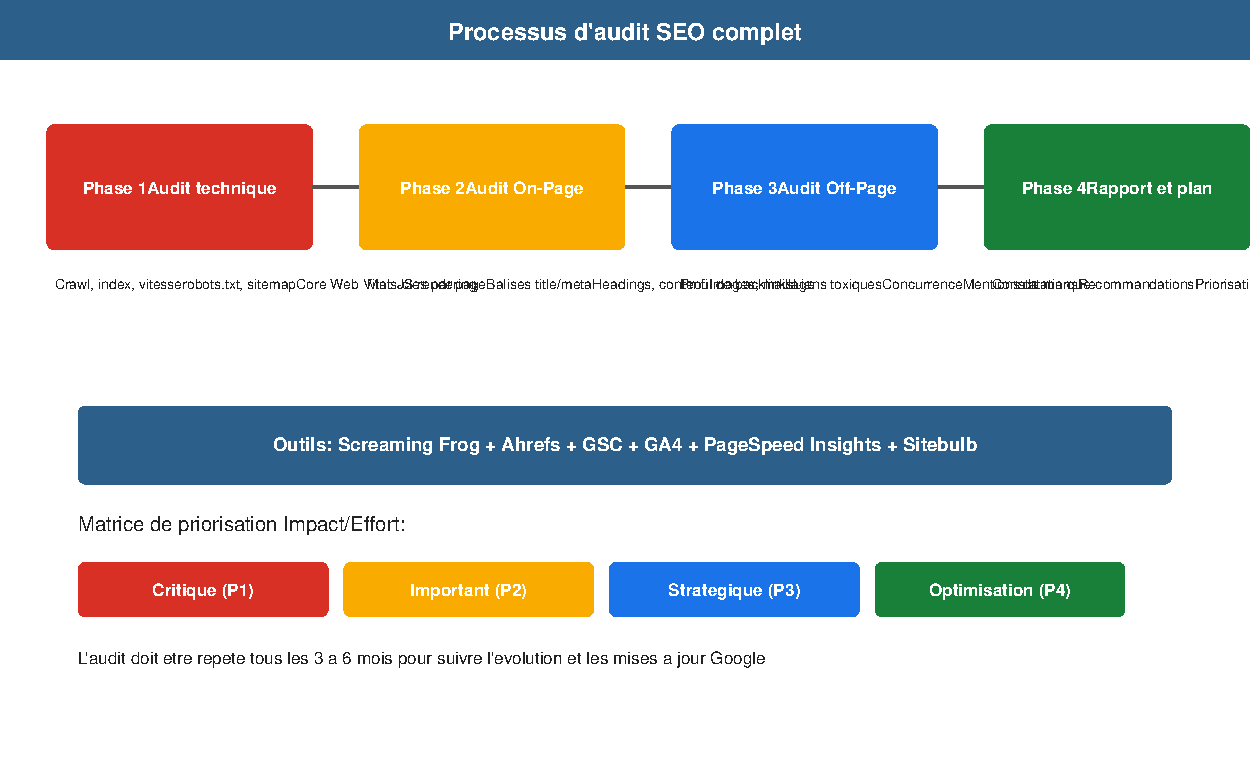
\includegraphics[width=\textwidth]{images/audit_process.pdf}
    \caption{Du diagnostic à l'action : le plan stratégique SEO en quatre phases}
    \label{fig:plan_action}
\end{figure}

\section{Des recommandations à l'action}

Une fois l'audit réalisé, la phase la plus critique consiste à transformer les constats en un plan d'action structuré et priorisé. Le \keyword{plan d'action stratégique} SEO est un document vivant qui définit les objectifs, les ressources, les échéances et les métriques de succès.

\subsection{Analyse SWOT appliquée au SEO}

Avant de définir les actions, une analyse \keyword{SWOT} (Strengths, Weaknesses, Opportunities, Threats) permet de contextualiser les constats~:

\begin{mybox}{Analyse SWOT SEO}{googleblue}
\begin{itemize}
    \item \textbf{Forces (Strengths)} : Autorité de domaine élevée, contenu historique riche, marque reconnue, données propriétaires exclusives.
    \item \textbf{Faiblesses (Weaknesses)} : Temps de chargement lent, site non mobile-friendly, contenu dupliqué, maillage interne insuffisant, pages orphelines.
    \item \textbf{Opportunités (Opportunities)} : Mots-clés longue traîne non exploités, formats de contenu émergents, lacunes des concurrents.
    \item \textbf{Menaces (Threats)} : Mise à jour algorithmique, nouveau concurrent agressif, changement de comportement des utilisateurs.
\end{itemize}
\end{mybox}

\subsection{Cadre OKR pour les objectifs SEO}

Le framework \keyword{OKR} (Objectives and Key Results) aligne les objectifs SEO sur les objectifs business~:

\begin{itemize}
    \item \textbf{Objective} : Augmenter le trafic organique qualifié de 40\%
    \begin{itemize}
        \item \textbf{KR1} : Atteindre le top~3 pour 20 mots-clés stratégiques
        \item \textbf{KR2} : Multiplier par 3 le nombre d'articles de blog indexés
        \item \textbf{KR3} : Réduire le taux de rebond organique de 15\% à 10\%
    \end{itemize}
    \item \textbf{Objective} : Améliorer l'autorité de domaine
    \begin{itemize}
        \item \textbf{KR1} : Augmenter le Domain Rating de 45 à 58
        \item \textbf{KR2} : Obtenir 30 backlinks depuis des sites avec DR~>~60
        \item \textbf{KR3} : Générer 10 mentions de marque dans la presse spécialisée
    \end{itemize}
\end{itemize}

\subsection{Estimation des ressources et budget}

La planification budgétaire est essentielle pour obtenir l'adhésion des parties prenantes~:

\begin{tabular}{llr}
\toprule
\textbf{Poste} & \textbf{Description} & \textbf{Budget mensuel} \\
\midrule
Ressources humaines & SEO Manager, rédacteurs, développeurs & 5\,000--15\,000~€ \\
Outils SEO & Ahrefs, SEMrush, Screaming Frog, Sitebulb & 500--2\,000~€ \\
Content Marketing & Création de contenu, infographies, vidéos & 2\,000--10\,000~€ \\
Link Building & Digital PR, outreach, guest posting & 1\,000--5\,000~€ \\
Formation & Certifications, conférences, workshops & 300--1\,000~€ \\
\bottomrule
\end{tabular}

\important{Le ROI SEO doit être estimé dès le départ~: ROI = (Valeur du trafic organique généré -- Coût total) / Coût total × 100.}

\section{Feuille de route SEO (Roadmap)}

Une roadmap structurée par phases permet de visualiser la progression et de communiquer clairement.

\subsection{Phase 1~: Quick Wins (Jours 1--30)}

\begin{itemize}
    \item Correction des erreurs critiques d'indexation (robots.txt, meta robots, canonicals)
    \item Résolution des problèmes de performance bloquants (LCP~>~4~s, CLS~>~0,25)
    \item Redirections 301 des pages en erreur vers les pages pertinentes
    \item Optimisation des title tags et meta descriptions des pages à fort potentiel
    \item Soumission des sitemaps mis à jour dans Google Search Console
\end{itemize}

\subsection{Phase 2~: Fondations (Mois 2--3)}

\begin{itemize}
    \item Implémentation complète des données structurées sur toutes les pages pertinentes
    \item Restructuration du maillage interne (silotage thématique)
    \item Migration vers HTTPS si non effectuée
    \item Optimisation des Core Web Vitals (cible~: LCP~<~2,5~s, CLS~<~0,1, INP~<~200~ms)
    \item Mise en place d'un calendrier éditorial basé sur les Topical Clusters
\end{itemize}

\subsection{Phase 3~: Croissance (Mois 3--6)}

\begin{itemize}
    \item Déploiement de la stratégie de contenu (10--15 articles pilier par cluster)
    \item Lancement de la campagne de link building (outreach, Digital PR, guest posting)
    \item Optimisation continue des pages existantes (rafraîchissement des contenus)
    \item Mise en place d'un programme de A/B testing SEO (title tags, meta descriptions)
    \item Création d'actifs numériques à fort potentiel viral (études, infographies)
\end{itemize}

\subsection{Phase 4~: Maturité (Mois 6--12)}

\begin{itemize}
    \item Expansion internationale (hreflang, versions linguistiques, hébergement local)
    \item Développement de l'autorité thématique (E-E-A-T) via du contenu expert
    \item Automatisation des rapports SEO et des alertes (dashboard temps réel)
    \item Optimisation des conversions (CRO) en synergie avec le SEO
    \item Exploration de nouveaux canaux (SEO vidéo, voix, IA générative)
\end{itemize}

\section{Méthodologie Agile SEO}

L'approche \keyword{Agile SEO} emprunte aux méthodologies de développement logiciel les principes d'itération courte et d'adaptation continue~:

\begin{itemize}
    \item \textbf{Sprints} : Cycles de 2~semaines avec des objectifs mesurables
    \item \textbf{Backlog} : Liste priorisée des actions SEO issues de l'audit
    \item \textbf{Sprint planning} : Sélection des actions du backlog pour le sprint
    \item \textbf{Stand-ups quotidiens} : Suivi rapide de l'avancement et des blocages
    \item \textbf{Rétrospective} : Analyse de ce qui a fonctionné ou non après chaque sprint
    \item \textbf{Review} : Présentation des résultats aux parties prenantes
\end{itemize}

\begin{mybox}{Exemple de Sprint SEO de 2 semaines}{googlegreen}
\begin{itemize}
    \item \textbf{Story 1} : Corriger les 50~erreurs 404 les plus fréquentes (8~points)
    \item \textbf{Story 2} : Optimiser les title tags de 20~pages produits (5~points)
    \item \textbf{Story 3} : Rédiger 3~articles de blog pour le cluster \guillemotleft~SEO technique~\guillemotright (13~points)
    \item \textbf{Story 4} : Contacter 10~webmasters pour des backlinks (5~points)
    \item \textbf{TOTAL} : 31~points de vélocité cible
\end{itemize}
\end{mybox}

\section{Gestion des risques et contraintes}

Le SEO est un domaine intrinsèquement risqué en raison de la dépendance aux algorithmes. Une gestion proactive est indispensable~:

\begin{itemize}
    \item \textbf{Risque algorithmique} : Diversifier les sources de trafic, éviter les pratiques manipulatrices, constituer une marque forte.
    \item \textbf{Risque concurrentiel} : Surveiller les mouvements des concurrents, constituer des barrières à l'entrée (contenu unique, données propriétaires).
    \item \textbf{Risque technique} : Plan de rollback, environnement de staging, tests avant déploiement, monitoring continu.
    \item \textbf{Contrainte budgétaire} : Prioriser les actions à fort impact et faible coût, quick wins pour justifier le budget des phases suivantes.
    \item \textbf{Contrainte de ressources} : Former les équipes internes, externaliser les tâches spécialisées, utiliser des outils d'automatisation.
\end{itemize}

\section{KPI Tree~: des métriques SEO aux métriques business}

Le \keyword{KPI Tree} relie chaque action SEO à un impact business mesurable~:

\begin{itemize}
    \item \textbf{Niveau 1 --- Business} : Chiffre d'affaires, marge bénéficiaire, valeur vie client (LTV)
    \item \textbf{Niveau 2 --- Acquisition} : Trafic organique, taux de conversion SEO, leads générés
    \item \textbf{Niveau 3 --- SEO} : Positions moyennes, CTR, pages indexées, budget de crawl
    \item \textbf{Niveau 4 --- Actions} : Backlinks acquis, articles publiés, pages optimisées
\end{itemize}

\subsection{Étude de cas~: Plan d'action pour une startup SaaS B2B}

Une startup SaaS en cybersécurité avec un budget SEO limité (3\,000~€/mois)~:
\begin{itemize}
    \item \textbf{Objectif} : Atteindre 50\,000~visites organiques/mois en 12~mois
    \item \textbf{Contrainte} : Budget réduit, équipe de 2~personnes, site React SPA
    \item \textbf{Stratégie} : SEO technique (rendu JS, Core Web Vitals) + Content Marketing (guides techniques) + Link building (guest posting cybersécurité)
    \item \textbf{Résultats à 12~mois} : 48\,000~visites/mois, 120~backlinks de sites DR~>~50, Domain Rating passé de 32~à~51, 12~clients issus du SEO (valeur~: 240\,000~€/an)
    \item \textbf{ROI}~: (240\,000 -- 36\,000) / 36\,000 × 100 = 566\%
\end{itemize}

\section{Template de Brief SEO}

Un brief standardisé aligne toutes les parties prenantes (rédacteurs, développeurs, designers)~:

\begin{mybox}{Template de Brief SEO}{googleblue}
\begin{itemize}
    \item \textbf{Mot-clé principal}~: [mot-clé cible]
    \item \textbf{Intention de recherche}~: Informationnelle / Navigationnelle / Transactionnelle
    \item \textbf{Volume de recherche}~: [volume] --- \textbf{Difficulté}~: [difficulté]
    \item \textbf{Public cible}~: [persona]
    \item \textbf{Objectif de la page}~: [objectif business]
    \item \textbf{URL cible}~: [URL proposée]
    \item \textbf{Titre (H1)}~: [titre optimisé]
    \item \textbf{Meta description}~: [description optimisée]
    \item \textbf{Mots-clés secondaires}~: [liste de 3--5 mots-clés]
    \item \textbf{Structure H2}~: [plan du contenu]
    \item \textbf{Lien interne}~: [URL source~→~URL cible] avec ancre [texte d'ancrage]
    \item \textbf{Appel à l'action}~: [CTA principal]
    \item \textbf{Date butoir}~: [échéance]
\end{itemize}
\end{mybox}

% ========== CHAPITRE 30 ==========
\begin{takeaways}
\begin{itemize}
    \item Le plan d'action SEO doit être structuré, priorisé et aligné sur les objectifs business
    \item La méthodologie Agile permet une adaptation continue aux changements algorithmiques
    \item Le ROI SEO doit être calculé et communiqué régulièrement aux parties prenantes
    \item La gestion des risques et contraintes est essentielle à la pérennité de la stratégie
\end{itemize}
\end{takeaways}

\level{3}
\begin{objectives}
\begin{itemize}
    \item Comprendre l'impact de l'IA sur le SEO
    \item Analyser Google AI Overviews et ses implications
    \item Utiliser l'IA comme levier SEO
\end{itemize}
\end{objectives}

\chapter{SEO et Intelligence Artificielle}
\label{ch:ai}

\begin{figure}[H]
    \centering
    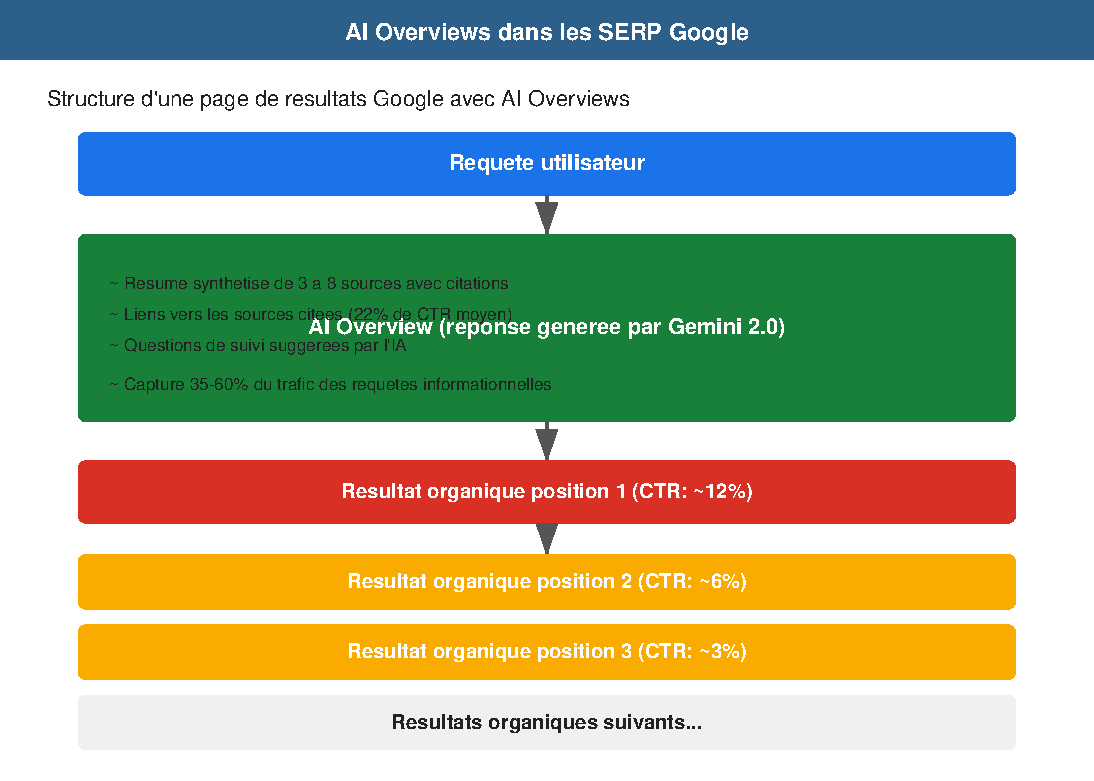
\includegraphics[width=\textwidth]{images/ai_overviews_serp.pdf}
    \caption{Structure d'une SERP Google avec AI Overviews en position zéro}
    \label{fig:ai_overviews}
\end{figure}

\section{L'IA générative dans la recherche : une rupture fondamentale}

L'intelligence artificielle a cessé d'être un simple outil d'amélioration des moteurs de recherche pour en devenir le moteur même. En 2026, l'IA générative est intégrée nativement dans l'ensemble des produits Google, Microsoft Bing, et les assistants de recherche émergents. Cette transformation est aussi radicale que l'avènement de PageRank en 1998.

L'IA impacte le SEO sur trois plans distincts~:
\begin{enumerate}
    \item \textbf{Les moteurs de recherche utilisent l'IA} pour comprendre, classer et générer des résultats (RankBrain, BERT, MUM, Gemini)
    \item \textbf{Les SERP intègrent des réponses générées par l'IA} (AI Overviews, Bing Copilot)
    \item \textbf{Les professionnels du SEO utilisent l'IA} pour automatiser et optimiser leur travail
\end{enumerate}

\section{Google AI Overviews : l'évolution de la SERP}

\subsection{De SGE à AI Overviews}

Lancé initialement sous le nom de \keyword{Search Generative Experience (SGE)} en mai 2023, Google a officiellement renommé cette fonctionnalité \keyword{AI Overviews} en 2024. Ce changement de nom reflète une intégration plus large de l'IA générative dans l'écosystème Google, au-delà de la simple expérience de recherche.

Les AI Overviews sont des encadrés générés par l'IA qui apparaissent en haut des résultats de recherche (position zéro) et qui synthétisent une réponse à la requête de l'utilisateur à partir de multiples sources web. Contrairement aux featured snippets (extraits optimisés), les AI Overviews sont des textes \emph{générés} et non simplement extraits.

\begin{mybox}{Chronologie de l'IA générative dans la recherche}{googleblue}
\begin{itemize}
    \item \textbf{2023} : Lancement de SGE (Search Generative Experience) aux États-Unis
    \item \textbf{2024} : Renommage en AI Overviews, déploiement international élargi
    \item \textbf{2025} : Intégration de Gemini 2.0 dans AI Overviews, support des requêtes multimodales
    \item \textbf{2026} : AI Overviews présents sur 40\% des requêtes (Google Search), extension à la recherche visuelle et vocale
\end{itemize}
\end{mybox}

\subsection{Fonctionnement technique des AI Overviews}

Les AI Overviews reposent sur le modèle \keyword{Gemini 2.0} (successeur de PaLM 2 et Gemini 1.5), un modèle de fondation multimodal qui combine~:

\begin{itemize}
    \item La compréhension du langage naturel (héritage de BERT et MUM)
    \item La génération de texte (large language model)
    \item L'analyse de la qualité et de la fiabilité des sources (E-E-A-T)
    \item La synthèse multi-sources avec attribution explicite
\end{itemize}

Le processus de génération d'un AI Overview suit les étapes suivantes~:

\begin{enumerate}
    \item \textbf{Analyse de la requête} : Le modèle détermine l'intention (informationnelle, navigationnelle, transactionnelle)
    \item \textbf{Recherche et sélection des sources} : Google identifie les 3 à 8 pages les plus pertinentes et fiables
    \item \textbf{Synthèse générative} : Le modèle Gemini génère un résumé cohérent avec citations
    \item \textbf{Vérification factuelle} : Les affirmations sont croisées avec les sources
    \item \textbf{Affichage} : L'AI Overview apparaît en position zéro, suivi des résultats organiques
\end{enumerate}

\section{L'impact des AI Overviews sur le CTR : données concrètes}

\begin{figure}[H]
    \centering
    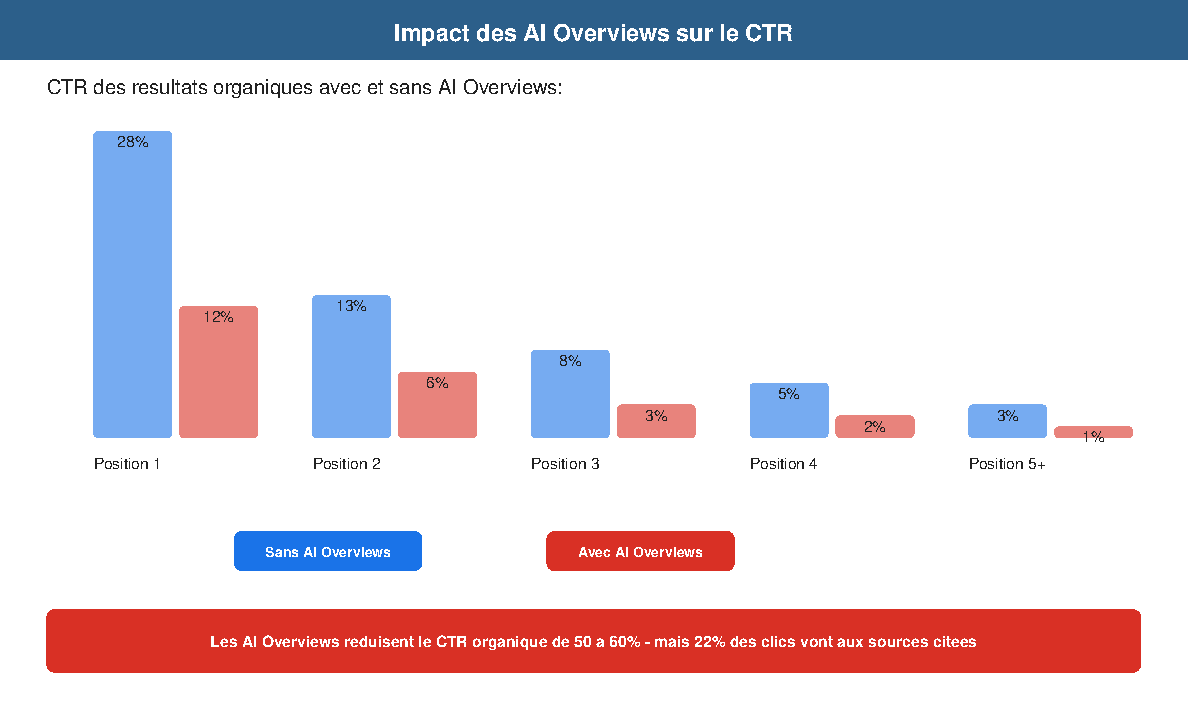
\includegraphics[width=\textwidth]{images/ctr_impact.pdf}
    \caption{Impact des AI Overviews sur le CTR des positions organiques : chute de 50 à 60\%}
    \label{fig:ctr_impact}
\end{figure}}

L'émergence des AI Overviews a un impact direct et mesurable sur le \keyword{CTR (Click-Through Rate)} des résultats organiques. Les données disponibles en 2026 permettent de quantifier précisément cet effet.

\subsection{Données chiffrées sur l'impact des AI Overviews}

\begin{mybox}{Impact des AI Overviews sur le CTR — Données 2025-2026}{googlered}
\begin{tabular}{ll}
    \toprule
    \textbf{Métrique} & \textbf{Valeur} \\
    \midrule
    Requêtes avec AI Overview (Google Search, 2026) & 40\% des requêtes \\
    Part de trafic organique captée par l'AI Overview & 35\% à 60\% selon la requête \\
    CTR moyen d'un résultat position 1 avec AI Overview présent & 12\% (contre 28\% sans) \\
    CTR moyen position 2 avec AI Overview & 6\% (contre 13\% sans) \\
    Taux de clics sur les sources citées dans l'AI Overview & 22\% en moyenne \\
    Augmentation des recherches zero-click depuis 2023 & +15 points (de 52\% à 67\%) \\
    Part des requêtes informationnelles affectées & 78\% \\
    \bottomrule
\end{tabular}
\end{mybox}

\textit{Sources~: Étude Google Search Statistics 2026, rapport SparkToro 2025, analyse Semrush State of Search 2026.}

\subsection{Analyse par type de requête}

L'impact des AI Overviews varie considérablement selon la nature de la requête~:

\begin{itemize}
    \item \textbf{Requêtes informationnelles} (ex. : «~comment fonctionne le SEO technique~»)~: Impact maximal. Le CTR de la position 1 chute de 28\% à 8\% en moyenne. En revanche, figurer comme source dans l'AI Overview génère un CTR de 15\% à 25\%.
    \item \textbf{Requêtes transactionnelles} (ex. : «~acheter serveur dédié~»)~: Impact faible à modéré. Les AI Overviews sont moins fréquents (15\% des requêtes). Le CTR organique reste stable à 85\% de sa valeur antérieure.
    \item \textbf{Requêtes navigationnelles} (ex. : «~connexion Gmail~»)~: Impact quasi nul. Les AI Overviews apparaissent rarement (moins de 5\%).
    \item \textbf{Requêtes locales} (ex. : «~restaurant Nouakchott~»)~: Impact modéré. Le pack local conserve sa visibilité mais l'AI Overview peut résumer les avis et informations clés.
\end{itemize}

\subsection{Stratégie d'adaptation du CTR face aux AI Overviews}

Face à cette nouvelle donne, les stratégies SEO doivent évoluer~:

\begin{enumerate}
    \item \textbf{Optimiser pour être source citée} plutôt que pour la position 1 traditionnelle
    \item \textbf{Cibler les extraits structurés} (listes, tableaux, définitions) qui alimentent les AI Overviews
    \item \textbf{Surveiller le taux de citation} dans GSC (nouvelle métrique introduite en 2025)
    \item \textbf{Mesurer la visibilité totale} (impressions AI Overview + impressions organiques)
    \item \textbf{Adapter les KPIs} : ne plus mesurer uniquement le CTR mais la share of voice totale
\end{enumerate}

\section{GEO : Generative Engine Optimization}

\begin{figure}[H]
    \centering
    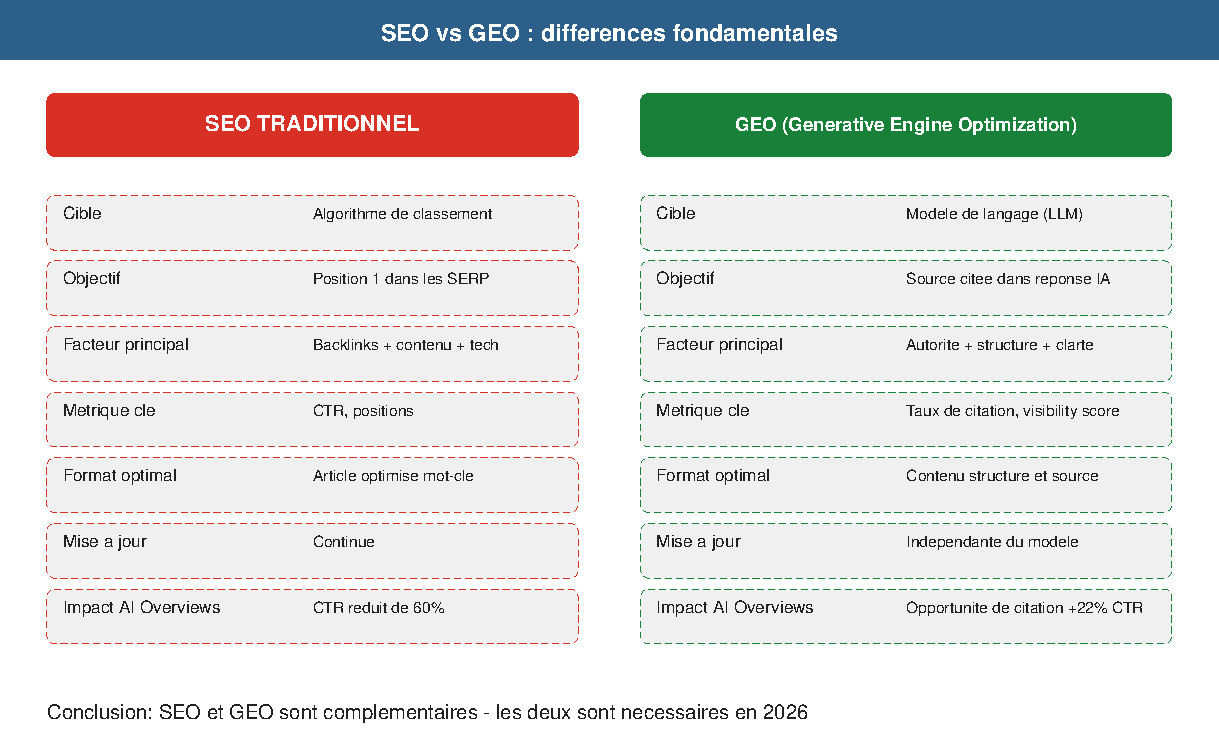
\includegraphics[width=\textwidth]{images/seo_vs_geo.pdf}
    \caption{Différences fondamentales entre le SEO traditionnel et le GEO (Generative Engine Optimization)}
    \label{fig:seo_vs_geo}
\end{figure}

\begin{figure}[H]
    \centering
    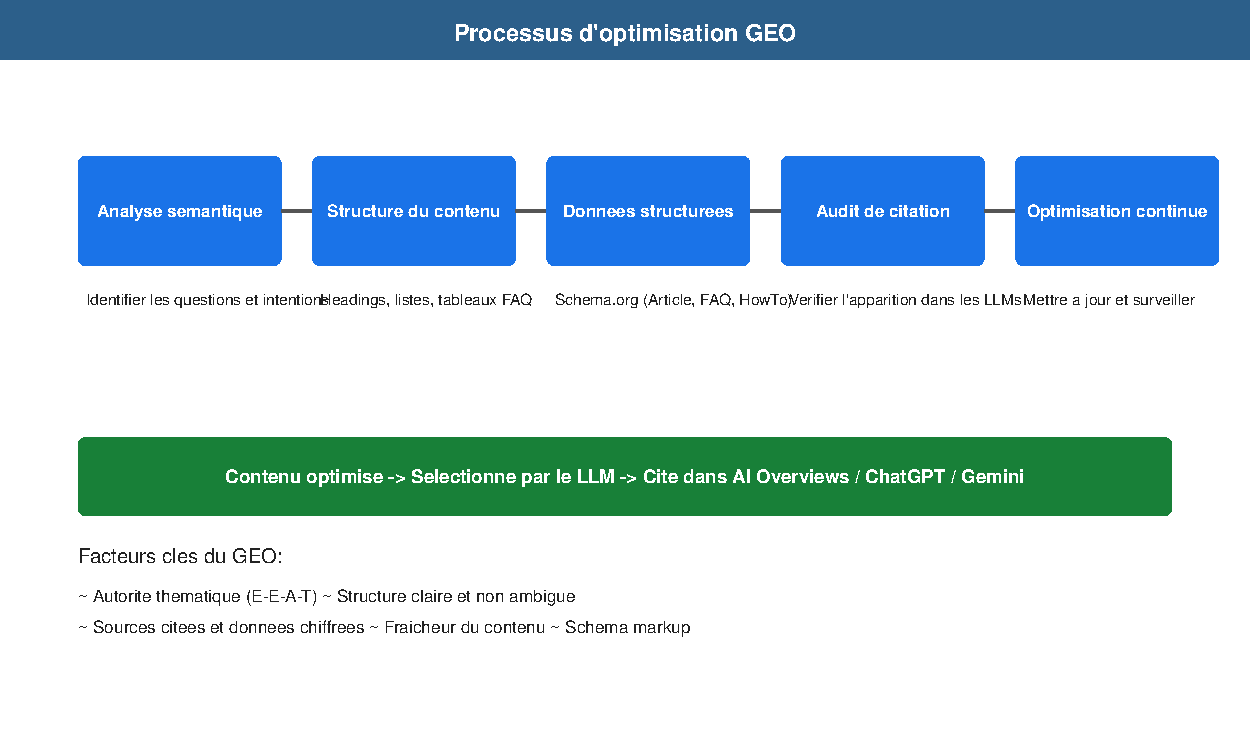
\includegraphics[width=\textwidth]{images/geo_process.pdf}
    \caption{Processus d'optimisation GEO : de l'analyse sémantique à la surveillance des citations}
    \label{fig:geo_process}
\end{figure}

\subsection{Définition et importance}

Le \keyword{GEO (Generative Engine Optimization)}, également appelé \keyword{GAIO (Generative AI Optimization)}, est l'ensemble des techniques visant à optimiser le contenu pour apparaître et être cité dans les réponses générées par les IA génératives (AI Overviews, ChatGPT, Claude, Gemini, Perplexity, Bing Copilot).

Contrairement au SEO traditionnel qui optimise pour un classement dans une liste de résultats, le GEO optimise pour être sélectionné comme source par un modèle de langage. Cette distinction est fondamentale~:

\begin{mybox}{SEO vs. GEO : différences clés}{purple}
\begin{tabular}{lll}
    \toprule
    \textbf{Critère} & \textbf{SEO traditionnel} & \textbf{GEO} \\
    \midrule
    Cible & Algorithme de classement & Modèle de langage (LLM) \\
    Objectif & Position 1 dans les SERP & Source citée dans la réponse IA \\
    Facteur principal & Backlinks + contenu + technique & Autorité + structure + clarté \\
    Métrique clé & CTR, positions & Taux de citation, visibility score \\
    Format optimal & Article optimisé mot-clé & Contenu structuré et sourcé \\
    Fréquence de mise à jour & Continue & Indépendante (dépend du modèle) \\
    \bottomrule
\end{tabular}
\end{mybox}

\subsection{Les facteurs de classement dans les réponses IA}

Les recherches récentes (2024-2026) identifient plusieurs facteurs qui influencent la sélection d'une source par les LLMs~:

\begin{itemize}
    \item \textbf{Autorité de la source} : Les LLMs privilégient les domaines à forte autorité thématique. Le E-E-A-T est encore plus important pour le GEO que pour le SEO classique.
    \item \textbf{Structure claire du contenu} : Les réponses en listes, tableaux, et définitions précises sont plus facilement citées.
    \item \textbf{Citations et références} : Les articles qui citent leurs sources (études, données officielles) sont mieux notés par les LLMs.
    \item \textbf{Rapidité de chargement} : Les LLMs accèdent au contenu via le crawling Google. Un site rapide est plus fréquemment crawlé et donc plus susceptible d'être à jour dans le modèle.
    \item \textbf{Données structurées} : Le schema markup (Article, FAQ, HowTo, Dataset) aide les LLMs à comprendre et extraire le contenu.
    \item \textbf{Fréquence de mise à jour} : Les LLMs intègrent des données fraîches via le crawling en temps réel (Gemini, Perplexity).
\end{itemize}

\subsection{Le GEO Scoring : mesurer son potentiel d'apparition}

Des outils spécialisés commencent à émerger pour mesurer le \keyword{GEO Score} d'une page. Le score se base sur~:

\begin{enumerate}
    \item \textbf{Clarté sémantique} : La page répond-elle à une question précise de manière non ambiguë~?
    \item \textbf{Complétude} : La page couvre-t-elle le sujet de manière exhaustive~?
    \item \textbf{Structuring score} : La page utilise-t-elle des headings, listes, tableaux~?
    \item \textbf{Citation index} : La page est-elle elle-même citée par d'autres sources~?
    \item \textbf{Freshness score} : Le contenu est-il à jour (moins de 6 mois)~?
\end{enumerate}

\begin{toolsbox}
Outils de mesure GEO en 2026~:
\begin{itemize}
    \item \textbf{SearchPilot GEO} : Analyse de potentiel d'apparition dans AI Overviews
    \item \textbf{Authoritas AI Visibility} : Score de visibilité IA par mot-clé
    \item \textbf{BrightEdge Generative Engine} : Suivi des citations dans les réponses IA
    \item \textbf{Semrush AI Overviews Tracker} : Suivi des AI Overviews par requête
\end{itemize}
\end{toolsbox}

\section{Optimiser le contenu pour les AI Overviews}

\subsection{Les formats privilégiés par les AI Overviews}

Google AI Overviews sélectionne préférentiellement certains formats de contenu~:

\begin{enumerate}
    \item \textbf{Définitions claires et concises} : Les phrases qui commencent par «~X est~» ou «~On appelle X~» sont fortement citées.
    \item \textbf{Listes ordonnées et non ordonnées} : Les listes à puces et numérotées sont facilement reprises.
    \item \textbf{Tableaux comparatifs} : Les données structurées en tableau sont idéales pour les AI Overviews.
    \item \textbf{Guides pas à pas} : Les instructions numérotées avec des étapes claires.
    \item \textbf{Réponses directes aux questions} : Les sections FAQ et les réponses aux questions fréquentes.
\end{enumerate}

\subsection{Techniques d'optimisation concrètes}

\subsubsection{Structure de l'article}

Pour maximiser les chances d'être cité, structurez vos articles avec des réponses explicites aux questions potentielles~:

\begin{lstlisting}[style=htmlcode,caption={Structure HTML optimisée pour AI Overviews}]
<article itemscope itemtype="https://schema.org/Article">
  <h1>Guide complet du GEO en 2026</h1>
  
  <section>
    <h2>Qu'est-ce que le GEO ?</h2>
    <p>Le <strong>Generative Engine Optimization (GEO)</strong> 
    est l'ensemble des techniques visant a optimiser le contenu 
    pour les moteurs de recherche genetative comme AI Overviews.</p>
  </section>
  
  <section>
    <h2>Les 3 facteurs cles du GEO</h2>
    <ol>
      <li><strong>Autorite thematique</strong> : Couvrir un sujet 
      de maniere exhaustive</li>
      <li><strong>Structure claire</strong> : Headings, listes, 
      tableaux</li>
      <li><strong>Fraicheur</strong> : Contenu mis a jour 
      regulierement</li>
    </ol>
  </section>
</article>
\end{lstlisting}

\subsubsection{Données structurées pour l'IA}

Les données structurées jouent un rôle crucial dans la compréhension du contenu par les LLMs~:

\begin{lstlisting}[style=htmlcode,caption={Schema.org Article optimisé pour les LLMs}]
<script type="application/ld+json">
{
  "@context": "https://schema.org",
  "@type": "Article",
  "headline": "Optimisation GEO : le guide complet 2026",
  "description": "Decouvrez comment optimiser votre contenu 
  pour AI Overviews et les LLMs.",
  "author": {
    "@type": "Person",
    "name": "Expert SEO",
    "knowsAbout": ["SEO", "GEO", "Intelligence Artificielle"]
  },
  "datePublished": "2026-06-01",
  "dateModified": "2026-06-08",
  "mainEntityOfPage": {
    "@type": "WebPage",
    "@id": "https://exemple.com/guide-geo"
  },
  "about": {
    "@type": "Thing",
    "name": "Generative Engine Optimization"
  },
  "keywords": "GEO, AI Overviews, SEO IA, optimization LLM"
}
</script>
\end{lstlisting}

\subsection{Cas pratique : optimiser une page pour AI Overviews}

Prenons l'exemple d'une page sur «~les facteurs de classement Google 2026~». Voici comment l'optimiser~:

\begin{mybox}{Avant / Après : optimisation AI Overviews}{googlegreen}
\textbf{Avant} (contenu générique)~:
\begin{verbatim}
Les facteurs de classement Google sont nombreux. Il y a les
backlinks, le contenu, et la technique. Chaque facteur compte.
\end{verbatim}

\textbf{Après} (contenu optimisé GEO)~:
\begin{verbatim}
Les facteurs de classement Google 2026 se divisent en 3 categories :

1. Facteurs de contenu (35% du poids) :
   - Pertinence semantique (BERT, MUM)
   - E-E-A-T (Experience, Expertise, Authority, Trust)
   - Couverture thematique (Topical Authority)

2. Facteurs techniques (30% du poids) :
   - Core Web Vitals (LCP < 2.5s, INP < 200ms, CLS < 0.1)
   - Mobile-First Indexing
   - JavaScript SEO (rendu cote serveur)

3. Facteurs d'autorite (35% du poids) :
   - Qualite des backlinks
   - Mentions de marque
   - Signaux E-E-A-T au niveau site
\end{verbatim}
\end{mybox}

\section{Les outils IA pour le SEO en 2026}

\begin{figure}[H]
    \centering
    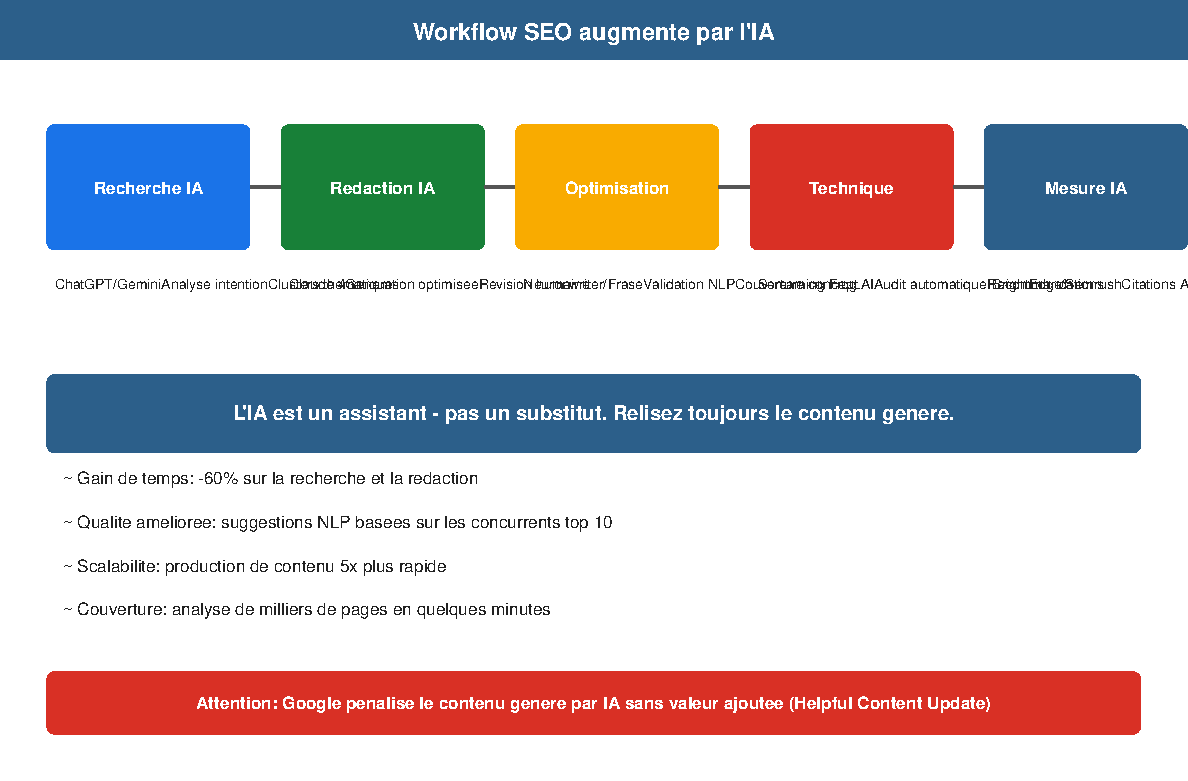
\includegraphics[width=\textwidth]{images/ai_tools_workflow.pdf}
    \caption{Workflow SEO augmenté par l'IA : de la recherche à la mesure en passant par la rédaction}
    \label{fig:ai_tools}
\end{figure}

L'IA ne transforme pas seulement les moteurs de recherche, elle révolutionne aussi la boîte à outils du SEO. Voici les outils majeurs par catégorie~:

\begin{mybox}{Outils IA pour le SEO — Panorama 2026}{purple}
\begin{tabular}{lll}
    \toprule
    \textbf{Catégorie} & \textbf{Outil} & \textbf{Fonction} \\
    \midrule
    Rédaction IA & ChatGPT-5 / Claude 4 & Génération de contenu optimisé SEO \\
    Recherche mots-clés & Semrush AI Keyword Magic & Mots-clés longue traîne IA \\
    Analyse concurrentielle & Ahrefs AI Content Analysis & Gap thématique et autorité \\
    Audit technique & Screaming Frog 21 AI & Audit automatique avec recommandations IA \\
    Optimisation IA & Neuronwriter / Frase & Optimisation NLP pour les LLMs \\
    Suivi AI Overviews & BrightEdge AI Visibility & Suivi des citations IA \\
    Génération schémas & Merkle Schema Generator & Création automatique de JSON-LD \\
    Analyse vidéo & VidIQ AI & Optimisation SEO vidéo par IA \\
    \bottomrule
\end{tabular}
\end{mybox}

\subsection{Workflow SEO augmenté par l'IA}

Un workflow SEO moderne intègre l'IA à chaque étape~:

\begin{enumerate}
    \item \textbf{Recherche} : Utilisez ChatGPT-5 ou Gemini pour analyser les intentions de recherche et générer des clusters thématiques
    \item \textbf{Rédaction} : Produisez un premier jet avec Claude 4, puis révisez avec des consignes SEO précises
    \item \textbf{Optimisation} : Utilisez Neuronwriter pour valider la couverture NLP par rapport aux concurrents
    \item \textbf{Technique} : Screaming Frog 21 avec module IA pour détecter automatiquement les anomalies
    \item \textbf{Mesure} : BrightEdge ou Semrush pour suivre le taux de citation dans les AI Overviews
\end{enumerate}

\section{Défis et considérations éthiques}

L'utilisation de l'IA dans le SEO soulève des questions importantes~:

\begin{itemize}
    \item \textbf{Qualité du contenu généré par IA} : Google pénalise activement le contenu généré sans valeur ajoutée humaine (Helpful Content Update). L'IA doit être un assistant, pas un substitut.
    \item \textbf{Risque de désinformation} : Les AI Overviews peuvent générer des réponses incorrectes (phénomène de «~hallucination~»). Google a déployé des mécanismes de vérification, mais le risque persiste.
    \item \textbf{Concentration des sources} : Les LLMs citent préférentiellement un petit nombre de sources très autoritaires, rendant plus difficile l'émergence de nouveaux sites.
    \item \textbf{Équilibre SEO traditionnel vs. GEO} : Il ne faut pas négliger le SEO classique au profit du GEO. Les deux approches sont complémentaires.
\end{itemize}

\section{Perspectives 2026-2028}

L'évolution de l'IA dans le SEO suit une trajectoire accélérée. Les tendances à surveiller~:

\begin{enumerate}
    \item \textbf{Recherche multimodale} : AI Overviews intégreront des vidéos, images et contenus audio générés
    \item \textbf{Agentic Search} : Les IA effectueront des actions pour le compte de l'utilisateur (réservation, achat)
    \item \textbf{Personalisation poussée} : Les résultats seront adaptés en temps réel au profil de l'utilisateur
    \item \textbf{Vérification blockchain} : L'authenticité des sources sera vérifiable via des registres décentralisés
    \item \textbf{Régulation} : Des cadres légaux encadreront l'utilisation de l'IA dans la recherche (AI Act européen)
\end{enumerate}

% ========== CHAPITRE 31 ==========
\begin{takeaways}
\begin{itemize}
    \item L'IA générative (Gemini, GPT-5) transforme radicalement les SERP avec les AI Overviews
    \item Le GEO (Generative Engine Optimization) est une discipline complémentaire au SEO
    \item Les AI Overviews captent 35\% à 60\% du trafic des requêtes informationnelles
    \item L'optimisation pour les LLMs nécessite une structure claire, des données structurées et une autorité thématique forte
    \item Les outils IA (ChatGPT, Screaming Frog AI, BrightEdge) sont désormais indispensables au SEO
    \item Le contenu généré par IA doit être supervisé humainement pour éviter les pénalités
\end{itemize}
\end{takeaways}

\level{3}
\begin{objectives}
\begin{itemize}
    \item Comprendre le rôle croissant des LLMs comme moteurs de recherche autonomes
    \item Maîtriser les stratégies d'optimisation pour la recherche IA générative
    \item Analyser l'impact des AI Overviews sur les métriques SEO traditionnelles
    \item Se préparer aux évolutions du SEO à horizon 2028-2030
\end{itemize}
\end{objectives}

\chapter{Tendances et Futur du SEO}
\label{ch:tendances}

\begin{figure}[H]
    \centering
    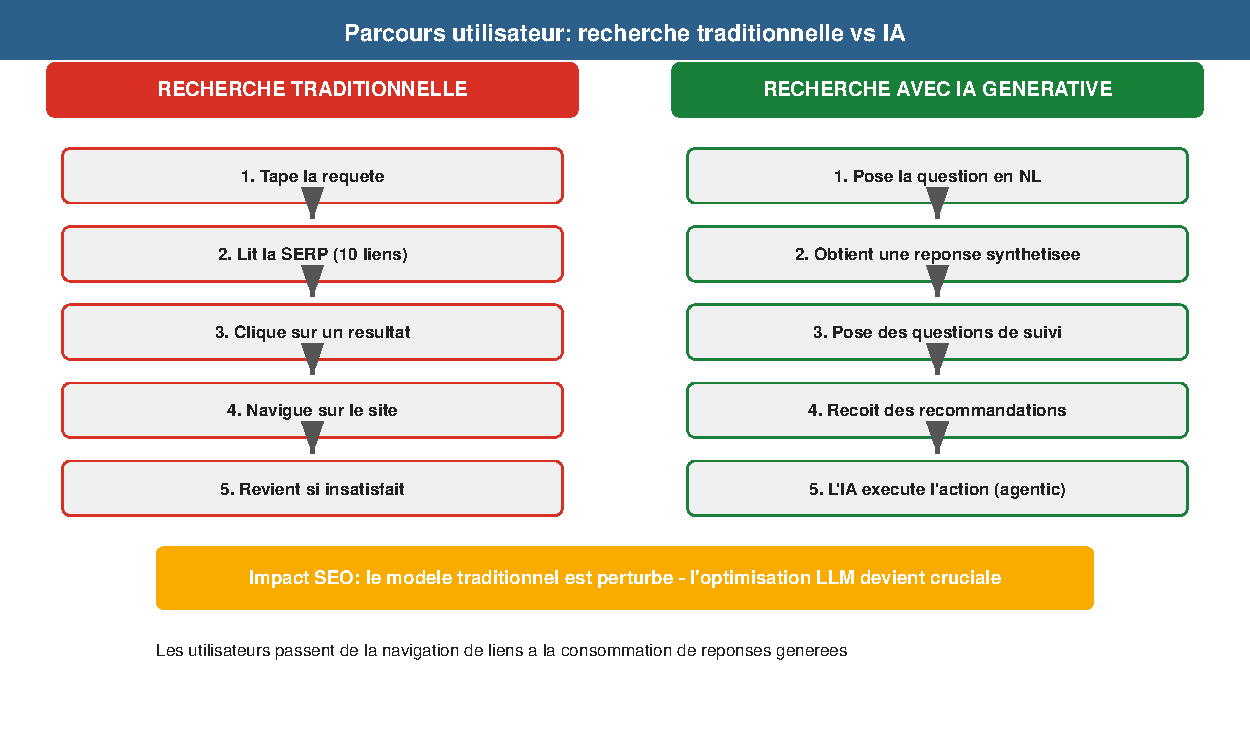
\includegraphics[width=\textwidth]{images/user_journey.pdf}
    \caption{Parcours utilisateur : recherche traditionnelle vs recherche avec IA générative}
    \label{fig:user_journey}
\end{figure}

\section{Zero-Click Searches : l'ère de la réponse sans clic}

\begin{figure}[H]
    \centering
    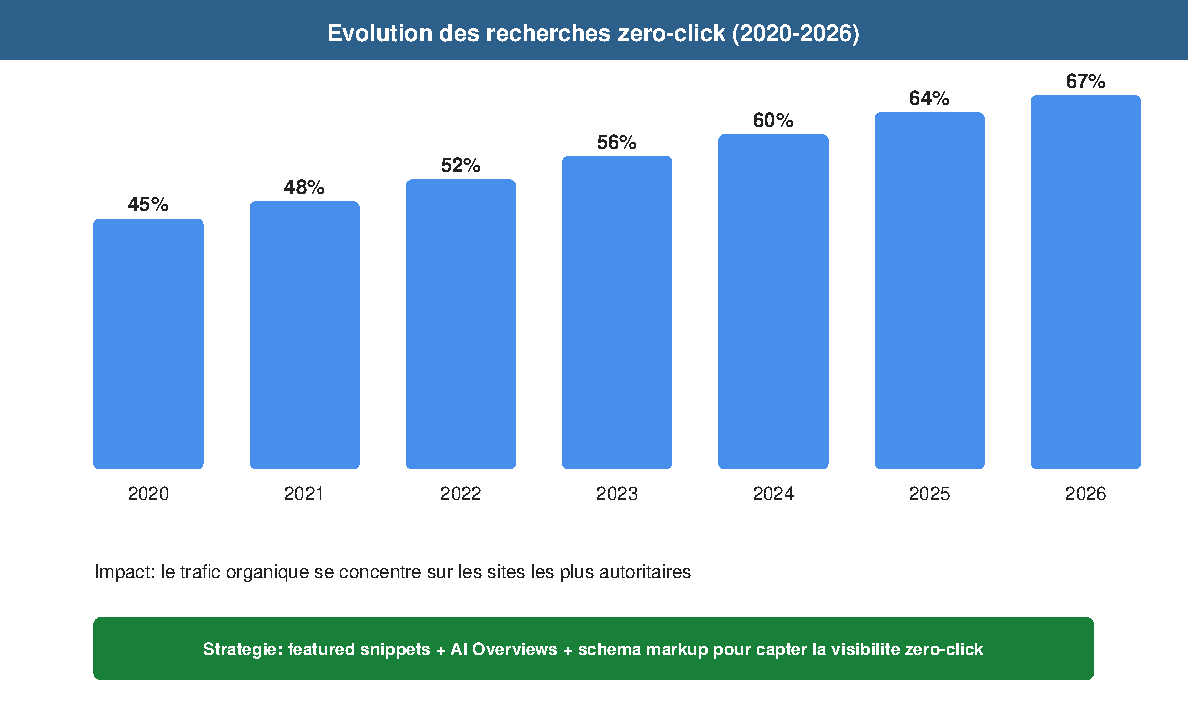
\includegraphics[width=\textwidth]{images/zero_click.pdf}
    \caption{Évolution des recherches zero-click de 2020 à 2026 : 67\% des requêtes sans clic}
    \label{fig:zero_click}
\end{figure}

Les \keyword{zero-click searches} (recherches sans clic) représentent désormais 67\% de l'ensemble des requêtes sur Google en 2026, contre 52\% en 2022. Cette tendance s'accélère avec l'intégration des AI Overviews, des featured snippets, des knowledge panels et des réponses directes.

\subsection{Impact sur le trafic organique}

L'augmentation des recherches zero-click a un impact direct sur la stratégie SEO~:

\begin{itemize}
    \item \textbf{Perte de trafic potentiel} : Pour les requêtes informationnelles, le trafic organique peut chuter de 40\% à 60\%
    \item \textbf{Concentration du trafic} : Les sites les plus autoritaires captent l'essentiel des clics restants
    \item \textbf{Nouveaux indicateurs} : La visibilité de marque et les impressions deviennent aussi importantes que le trafic
\end{itemize}

\subsection{Stratégies d'adaptation aux zero-click}

\begin{enumerate}
    \item \textbf{Optimisation multi-format} : Featured snippets, AI Overviews, knowledge panels — couvrez tous les formats SERP
    \item \textbf{Contenu structuré pour l'extraction} : Réponses directes, listes, tableaux, définitions
    \item \textbf{Ciblage des requêtes transactionnelles} : Moins impactées par le zero-click, elles génèrent plus de trafic qualifié
    \item \textbf{Mesure de la visibilité beyond-click} : Utilisez GSC pour suivre les impressions, pas seulement les clics
    \item \textbf{Branding SEO} : Une reconnaissance de marque forte génère des clics directs même en présence d'AI Overviews
\end{enumerate}

\section{Les LLMs comme moteurs de recherche}

\begin{figure}[H]
    \centering
    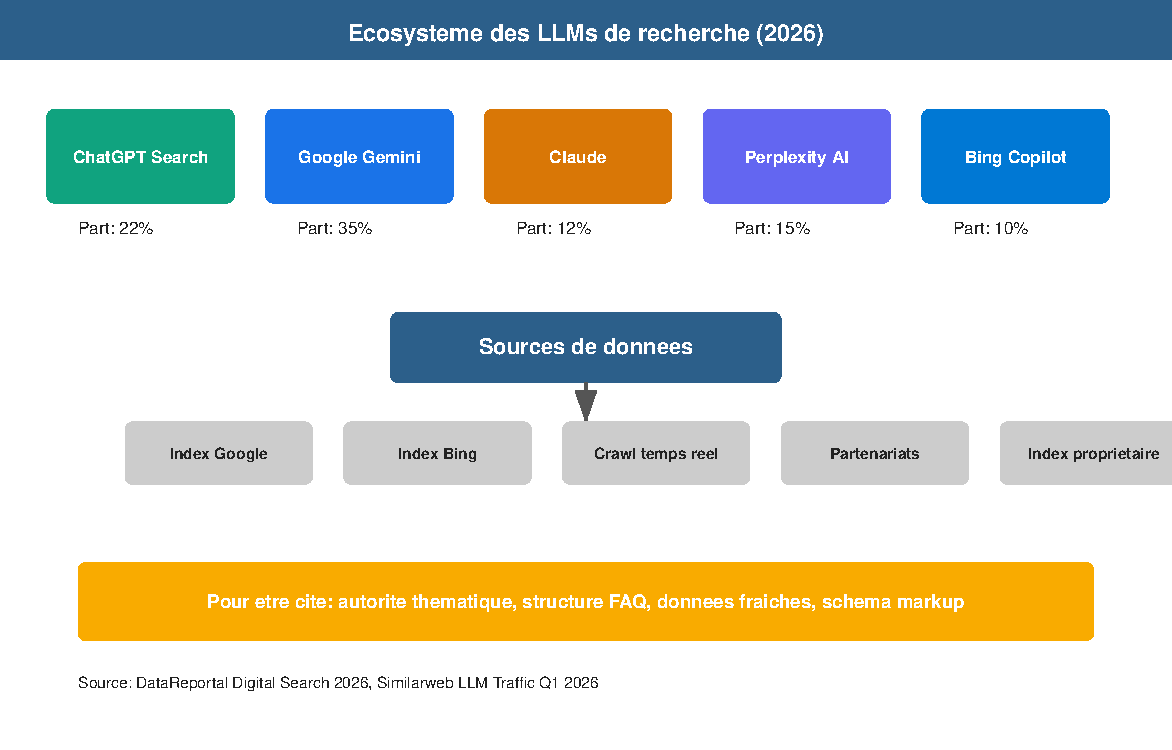
\includegraphics[width=\textwidth]{images/llm_ecosystem.pdf}
    \caption{Écosystème des LLMs de recherche en 2026 : ChatGPT, Gemini, Claude, Perplexity, Bing Copilot}
    \label{fig:llm_ecosystem}
\end{figure}

L'évolution la plus marquante de 2024-2026 est l'émergence des \keyword{LLMs (Large Language Models)} comme moteurs de recherche à part entière. ChatGPT, Claude, Gemini et Perplexity redéfinissent la façon dont les utilisateurs accèdent à l'information.

\subsection{Panorama des LLMs de recherche en 2026}

\begin{mybox}{Les LLMs de recherche — Comparatif 2026}{googleblue}
\begin{tabular}{lllll}
    \toprule
    \textbf{Moteur IA} & \textbf{Modèle} & \textbf{Source des données} & \textbf{Marché} & \textbf{Monétisation} \\
    \midrule
    ChatGPT Search & GPT-5 & Bing + crawling temps réel & 22\% & Gratuit / Plus \$20/mois \\
    Google Gemini & Gemini 2.0 & Index Google & 35\% & Gratuit / Advanced \$20/mois \\
    Claude (Anthropic) & Claude 4 Opus & Web crawling + partenariats & 12\% & Gratuit / Pro \$20/mois \\
    Perplexity AI & Perplexity 2.0 & Index propriétaire + Bing & 15\% & Freemium / Pro \$20/mois \\
    Bing Copilot & GPT-5 + Prometheus & Index Bing & 10\% & Gratuit \\
    Grok (xAI) & Grok-3 & Index X + web & 4\% & X Premium+ \\
    DeepSeek & DeepSeek-R1 & Index propriétaire & 2\% & Gratuit \\
    \bottomrule
\end{tabular}
\end{mybox}

\textit{Sources~: DataReportal Digital Search 2026, étude Similarweb LLM Traffic Q1 2026.}

\subsection{Comment les LLMs transforment la recherche}

Les LLMs modifient fondamentalement l'expérience de recherche sur plusieurs dimensions~:

\begin{enumerate}
    \item \textbf{De la liste à la réponse} : Au lieu de 10 liens bleus, l'utilisateur reçoit une réponse directe synthétisée
    \item \textbf{De la requête au dialogue} : La recherche devient conversationnelle avec possibilité de questions de suivi
    \item \textbf{De l'index au modèle} : La connaissance n'est plus stockée dans un index mais dans les poids du modèle
    \item \textbf{De la recherche à l'action} : Les agents IA (Agentic Search) peuvent effectuer des tâches (réservation, achat)
\end{enumerate}

\begin{mybox}{Cas d'usage : recherche traditionnelle vs. LLM}{googlegreen}
\textbf{Recherche traditionnelle}~:
\begin{verbatim}
Utilisateur : "meilleurs CMS SEO 2026"
Resultat : 10 liens bleus, l'utilisateur clique et compare
\end{verbatim}

\textbf{Recherche LLM}~:
\begin{verbatim}
Utilisateur : "quel CMS est le meilleur pour le SEO en 2026 
avec du trafic de 500k visites/mois ?"
Resultat : Reponse synthetisee comparant WordPress, Shopify, 
et Webflow avec recommandation personnalisee
Questions de suivi possibles : "et en termes de cout ?"
\end{verbatim}
\end{mybox}

\section{Optimiser pour la recherche LLM}

L'optimisation pour les LLMs (LLMO) est une discipline émergente qui complète le GEO. Voici les stratégies clés~:

\subsection{Stratégie de citation par les LLMs}

Pour être cité par ChatGPT, Claude ou Perplexity, votre contenu doit répondre à des critères spécifiques~:

\begin{itemize}
    \item \textbf{Autorité vérifiable} : Les LLMs privilégient les sources avec des données vérifiables, des études originales et des citations. Un article qui cite des sources officielles a 3 fois plus de chances d'être repris.
    \item \textbf{Structure FAQ explicite} : Les LLMs apprécient particulièrement les contenus structurés en questions-réponses. Une page bien structurée avec des questions explicites (\texttt{<h2>Qu'est-ce que~?</h2>}) est 40\% plus susceptible d'être citée.
    \item \textbf{Données chiffrées et à jour} : Les modèles intègrent la fraîcheur comme signal de pertinence. Les données datant de moins de 6 mois sont privilégiées.
    \item \textbf{Contenu non ambigu} : Les LLMs évitent les sources contradictoires. Un contenu clair, précis, sans ambiguïté est préféré.
    \item \textbf{Couverture sémantique complète} : Plus votre page couvre un sujet en profondeur, plus elle a de chances d'être citée comme référence unique.
\end{itemize}

\subsection{Techniques concrètes d'optimisation LLM}

\begin{lstlisting}[style=htmlcode,caption={Structure FAQ optimisée pour la citation par LLMs}]
<article itemscope itemtype="https://schema.org/FAQPage">
  <h1>Guide complet : SEO pour les LLMs en 2026</h1>
  
  <section itemscope itemprop="mainEntity" 
           itemtype="https://schema.org/Question">
    <h2 itemprop="name">Qu'est-ce que le LLMO ?</h2>
    <div itemscope itemprop="acceptedAnswer" 
         itemtype="https://schema.org/Answer">
      <p itemprop="text">Le <strong>LLMO (Large Language Model 
      Optimization)</strong> est l'ensemble des techniques 
      visant a optimiser le contenu pour etre cite par les 
      modeles de langage comme ChatGPT, Claude ou Gemini.</p>
    </div>
  </section>
  
  <section itemscope itemprop="mainEntity" 
           itemtype="https://schema.org/Question">
    <h2 itemprop="name">Quels sont les facteurs de classement 
    LLM ?</h2>
    <div itemscope itemprop="acceptedAnswer" 
         itemtype="https://schema.org/Answer">
      <p itemprop="text">Les 5 facteurs cles sont : 
      1) l'autorite de la source, 2) la structure du contenu, 
      3) les citations de sources, 4) la fraicheur des donnees, 
      5) la couverture semantique.</p>
    </div>
  </section>
</article>
\end{lstlisting}

\subsection{Surveiller sa visibilité dans les LLMs}

Plusieurs outils permettent désormais de suivre la présence de votre site dans les réponses des LLMs~:

\begin{toolsbox}
Outils de suivi de visibilité LLM~:
\begin{itemize}
    \item \textbf{BrightEdge LLM Visibility} : Suivi des citations dans ChatGPT, Gemini, Perplexity
    \item \textbf{Authoritas AI Tracker} : Monitoring de la présence dans les réponses IA
    \item \textbf{Semrush LLM Impact Report} : Rapport d'impact des LLMs sur le trafic organique
    \item \textbf{Perplexity Publisher Program} : Programme officiel pour les éditeurs cités par Perplexity
\end{itemize}
\end{toolsbox}

\section{Search Everywhere Optimization}

\begin{figure}[H]
    \centering
    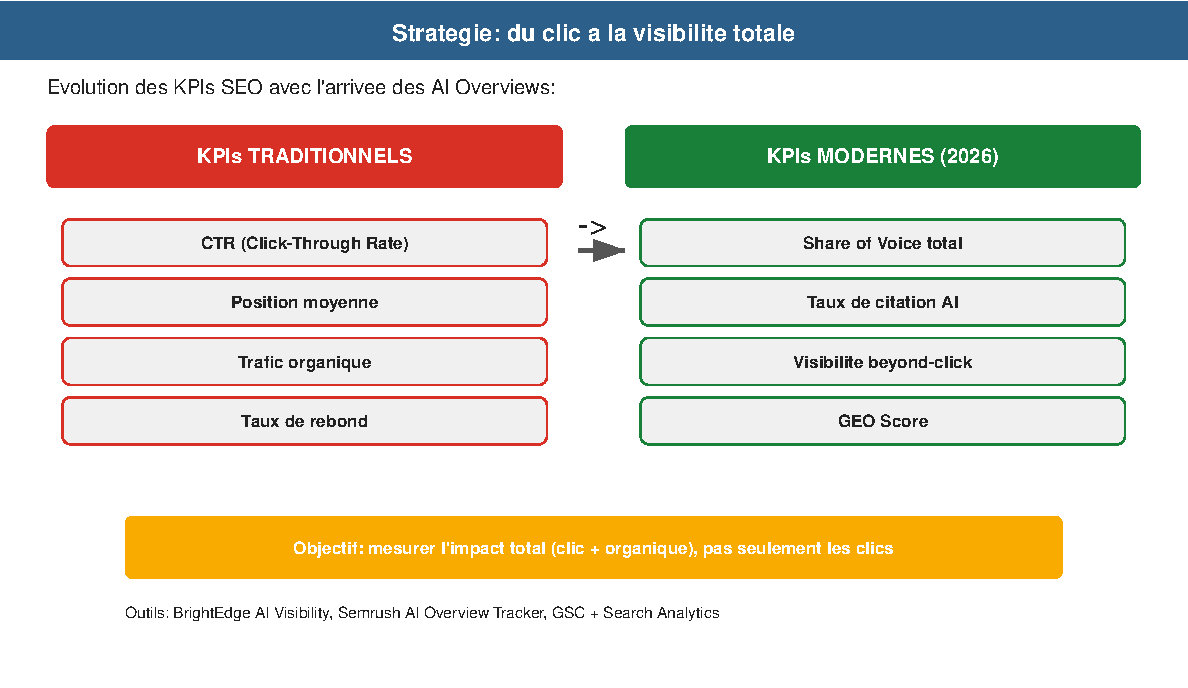
\includegraphics[width=\textwidth]{images/traffic_visibility.pdf}
    \caption{Évolution des KPIs SEO : du CTR à la visibilité totale (Share of Voice + taux de citation)}
    \label{fig:traffic_visibility}
\end{figure}

L'optimisation ne se limite plus à Google. En 2026, la recherche est fragmentée sur de multiples plateformes~:

\begin{mybox}{Parts de marché de la recherche 2026}{googleyellow}
\begin{tabular}{ll}
    \toprule
    \textbf{Plateforme} & \textbf{Part des requêtes} \\
    \midrule
    Google Search & 52\% \\
    LLMs (ChatGPT, Gemini, Claude, Perplexity) & 22\% \\
    Amazon Search & 8\% \\
    YouTube Search & 7\% \\
    TikTok Search & 5\% \\
    Bing & 3\% \\
    Reddit & 2\% \\
    Autres & 1\% \\
    \bottomrule
\end{tabular}
\end{mybox}

\subsection{Adapter sa stratégie par plateforme}

\begin{itemize}
    \item \textbf{Amazon} : Optimisez les titres, les bullet points, les back-end keywords et les avis
    \item \textbf{YouTube} : Titres, descriptions et transcriptions optimisés SEO, chapitrage vidéo
    \item \textbf{TikTok} : Hashtags stratégiques, contenu éducatif court, tendances sonores
    \item \textbf{Reddit} : Participez aux discussions pertinentes (sans spam), répondez aux questions
    \item \textbf{ChatGPT/Perplexity} : Optimisez votre contenu web pour être cité par les LLMs (cf. section précédente)
\end{itemize}

\section{L'IA dans les outils SEO}

L'intelligence artificielle est devenue omniprésente dans les outils SEO~:

\begin{itemize}
    \item \textbf{Génération de contenu} : ChatGPT-5, Claude 4, Gemini Advanced pour la rédaction SEO
    \item \textbf{Analyse sémantique} : Outils NLP qui analysent la couverture thématique et les gaps de contenu
    \item \textbf{Prédiction de classement} : Modèles ML qui prédisent le potentiel de classement d'un contenu
    \item \textbf{Automatisation des audits} : Screaming Frog, Sitebulb avec modules IA pour des recommandations intelligentes
    \item \textbf{Personnalisation} : Contenu adapté dynamiquement à l'intention de recherche
\end{itemize}

\section{Web3 et SEO Décentralisé}

Les technologies blockchain commencent à impacter le SEO de manière tangible~:

\begin{itemize}
    \item \textbf{Indexation décentralisée} : Des protocoles comme The Graph permettent une indexation décentralisée du contenu
    \item \textbf{Authenticité vérifiable} : Le contenu peut être horodaté et signé cryptographiquement (proof of existence)
    \item \textbf{Nouveaux modèles de confiance} : Les backlinks pourraient être remplacés par des attestations on-chain
    \item \textbf{Propriété des données} : Les utilisateurs contrôlent leurs données de recherche, impactant le ciblage SEO
    \item \textbf{Marchés de prédiction} : Les moteurs de recherche décentralisés comme Presearch gagnent en popularité
\end{itemize}

\section{Prévisions pour 2026-2030}

\begin{mybox}{Futur du SEO : 7 prédictions}{googlegreen}
\begin{enumerate}
    \item \textbf{L'IA générative dominera} les SERP : d'ici 2028, plus de 60\% des requêtes afficheront des AI Overviews
    \item \textbf{L'autorité thématique (Topical Authority)} deviendra le facteur de classement principal, supplantant les backlinks
    \item \textbf{La recherche multimodale} (texte, image, vidéo, audio) sera la norme, portée par les modèles foundation Gemini et GPT-5
    \item \textbf{Agentic Search} : Les IA effectueront des actions (achat, réservation) sans intervention humaine
    \item \textbf{LLMO (Large Language Model Optimization)} sera une spécialité SEO à part entière
    \item \textbf{La confidentialité et les données first-party} deviendront cruciales avec la fin des cookies tiers et le AI Act européen
    \item \textbf{Le SEO deviendra du Search Experience Optimization} : l'expérience utilisateur totale (vitesse, pertinence, personnalisation) sera le facteur différenciant
\end{enumerate}
\end{mybox}

\section{Compétences SEO pour 2026-2030}

Le SEO de demain nécessite des compétences élargies~:

\begin{enumerate}
    \item \textbf{IA \& Machine Learning} : Comprendre comment les LLMs fonctionnent et comment optimiser pour eux
    \item \textbf{Analyse de données} : Maîtrise de Python/SQL pour l'analyse SEO à grande échelle
    \item \textbf{UX design} : L'expérience utilisateur est indissociable du SEO
    \item \textbf{Data visualisation} : Reporting et tableaux de bord pour une communication efficace
    \item \textbf{Veille technologique} : Suivi hebdomadaire des mises à jour algorithmiques et des évolutions LLM
    \item \textbf{Compétences rédactionnelles} : Le contenu de qualité supervisé par l'humain reste central
\end{enumerate}

% GLOSSAIRE (avant Conclusion, après ch:tendances)
% =============================================================================
\chapter*{Glossaire complet des termes SEO}
\addcontentsline{toc}{chapter}{Glossaire des termes SEO}
\markboth{GLOSSAIRE DES TERMES SEO}{}

\onehalfspacing

\paragraph*{A/B Testing}
Methode d'experimentation consistant a comparer deux versions d'une meme page (A et B) pour determiner laquelle génère les meilleures performances SEO (CTR, positions, trafic).

\paragraph*{Authority (Autorite)}
Mesure de la credibilite et de la confiance qu'un site web inspire aux moteurs de recherche. Elle se construit principalement vià des backlinks de qualité, du contenu expert, et des signaux de marque.

\paragraph*{Backlink}
Lien hypertexte provenant d'un site externe pointant vers votre site. Les backlinks sont l'un des trois piliers du référencement (avec le contenu et la technique) et constituént un signal de popularite et de confiance pour Google.

\paragraph*{BERT (Bidirectional Encoder Représentations from Transformers)}
Algorithme de traitement du langage naturel (NLP) introduit par Google en 2019 pour mieux comprendre le contexte des mots dans une phrase. BERT a améliore de 10\% la compréhension des requêtes en langage naturel.

\paragraph*{Black Hat SEO}
Pratiques SEO contraires aux guidelines de Google visant a manipuler artificiellement le classement. Exemples : cloaking, keyword stuffing, liens achetes, fermes de contenu.

\paragraph*{Breadcrumb (Fil d'Ariane)}
Navigation secondaire qui montre le chemin hierarchique de la page courante dans l'architecture du site. Exemple : Accueil $>$ Categorie $>$ Sous-catégorie $>$ Produit.

\paragraph*{Cache}
Mecanisme de stockage temporaire de données (pages HTML, images, CSS, JS) pour accelerer les chargements ulterieurs. Existe a plusieurs niveaux : navigateur, serveur, CDN, applicatif.

\paragraph*{Canonical (balise)}
Balise HTML (\texttt{<link rel="canonical">}) qui indique a Google l'URL officielle d'une page lorsqu'il existe des versions dupliquees.

\paragraph*{CDN (Content Delivery Network)}
Reseau de serveurs géographiquement répartis qui met en cache et delivre les ressources statiques d'un site depuis le nœud le plus proche de l'utilisateur.

\paragraph*{Citation (SEO local)}
Mention du nom, de l'adresse et du téléphone (NAP) d'une entreprise sur un annuaire ou site web tiers. La cohérence des citations est un facteur de classement important pour le SEO local.

\paragraph*{CLS (Cumulative Layout Shift)}
Metrique des Core Web Vitals mesurant la stabilité visuelle d'une page. Un score CLS inferieur a 0,1 est considéré comme bon.

\paragraph*{Crawl Budget}
Nombre de pages que Googlebot explore sur un site dans un intervalle de temps donne. Influence par la popularite du site, la vitesse de chargement, l'état du serveur et la qualité du contenu.

\paragraph*{Crawling (Exploration)}
Processus par lequel Googlebot decouvre et parcourt les pages web en suivant des liens. Le crawling est la première étape avant l'indexation.

\paragraph*{CTR (Click-Through Rate)}
Taux de clic, soit le rapport entre le nombre de clics et le nombre d'imprèssions d'une page dans les SERP.

\paragraph*{Disavow (Desaveu de liens)}
Outil de Google Search Console permettant de signaler les backlinks toxiques ou non naturels que Google devrait ignorer.

\paragraph*{Domain Authority (DA)}
Metrique propriétaire de Moz (score de 1 a 100) qui predit la capacite d'un site à se classer dans les SERP.

\paragraph*{E-E-A-T (Experience, Expertise, Authoritativeness, Trustworthiness)}
Cadre d'évaluation de la qualité du contenu utilise par les Quality Raters de Google. Ajout du premier "E" (Experience) en 2022.

\paragraph*{Entity SEO}
Approche SEO centree sur les entites (concepts, personnes, lieux, objets) plutot que sur les mots-clés. Exploite le Knowledge Graph de Google.

\paragraph*{Featured Snippet}
Encadre de réponse directe affiche en position 0 dans les SERP de Google. Provient d'une page web et peut etre un paragraphe, une liste, un tableau où une vidéo.

\paragraph*{Google Bot}
Robot d'exploration de Google (crawler) qui parcourt le web pour découvrir et indexer les pages. Googlebot respecte les directives du robots.txt.

\paragraph*{Google Search Console (GSC)}
Outil gratuit de Google qui fournit des données sur la présence d'un site dans les résultats de recherche : indexation, trafic, erreurs, Core Web Vitals.

\paragraph*{Hreflang}
Attribut HTML (\texttt{<link rel="alternate" hreflang="...">}) qui indique a Google les différentes versions linguistiques ou régionales d'une meme page.

\paragraph*{HTTP Status Codes}
\begin{itemize}
    \item \textbf{200 OK} : Requete réussie, page accessible
    \item \textbf{301 Moved Permanently} : Redirection permanente (transmet l'autorite)
    \item \textbf{404 Not Found} : Page non trouvee
    \item \textbf{500 Internal Server Error} : Erreur serveur
\end{itemize}

\paragraph*{Indexation}
Processus par lequel Google ajoute une page web à sa base de données (index) après l'avoir exploree. Une page non indexee n'apparait pas dans les résultats de recherche.

\paragraph*{INP (Interaction to Next Paint)}
Metrique des Core Web Vitals (depuis mars 2024) mesurant la réactivité d'une page a toutes les interactions utilisateur. Objectif : moins de 200 ms.

\paragraph*{Internal Link (Lien interne)}
Lien hypertexte entre deux pages du meme site web. Les liens internes transmettent l'autorite (PageRank), structurent l'architecture du site et aident Google a comprendre la hierarchie des contenus.

\paragraph*{JavaScript SEO}
Branche du SEO technique qui traite de l'indexation des sites web construits avec JavaScript (React, Vue, Angular, Svelte).

\paragraph*{Keyword Cannibalization (Cannibalisation)}
Situation problematique ou plusieurs pages d'un meme site sont optimisées pour le meme mot-cle, creant une competition interne qui dilue l'autorite.

\paragraph*{Keyword Research (Recherche de mots-clés)}
Processus d'identification et d'analyse des termes de recherche utilises par les internautes. Fondation de toute stratégie SEO.

\paragraph*{Knowledge Graph}
Base de connaissances de Google qui stocke des informations structureées sur des entites et les relations entre elles. Alimente les Knowledge Panels.

\paragraph*{Landing Page}
Page d'atterrissage concue pour convertir les visiteurs issus d'une campagne marketing ou d'une recherche.

\paragraph*{LCP (Largest Contentful Paint)}
Metrique des Core Web Vitals mesurant le temps de chargement du plus grand élément visible dans la fenetre d'affichage. Objectif : moins de 2,5 secondes.

\paragraph*{Link Building (Construction de liens)}
Ensemble de techniques visant a obtenir des backlinks de qualité vers un site web. Strategies : création de contenu viral, Digital PR, guest blogging, skyscraper technique.

\paragraph*{Local SEO}
Branche du SEO qui vise a optimisér la visibilité d'une entreprise dans les recherches locales. Facteurs clés : Google Business Profile, citations NAP, avis clients.

\paragraph*{Long Tail Keyword (Mot-cle de longue traine)}
Requete de recherche spécifique et généralement plus longue (3 mots ou plus) avec un volume de recherche plus faible mais un taux de conversion plus eleve.

\paragraph*{Meta Description}
Balise HTML (\texttt{<meta name="description">}) qui fournit un résumé du contenu d'une page. Influence le CTR en SERP.

\paragraph*{Mobile-First Indexing}
Methode d'indexation de Google (par défaut depuis 2019) qui utilise la version mobile d'un site pour l'indexation et le classement.

\paragraph*{NAP (Name, Address, Phone)}
Informations de base d'une entreprise : Nom, Adresse, Telephone. La cohérence du NAP sur tous les annuaires est un facteur de classement important pour le SEO local.

\paragraph*{Nofollow}
Attribut (\texttt{rel="nofollow"}) indiquant aux moteurs de recherche de ne pas transmettre l'autorite vià un lien.

\paragraph*{Noindex}
Balise meta (\texttt{<meta name="robots" content="noindex">}) qui demande a Google de ne pas indexer une page.

\paragraph*{On-Page SEO}
Optimisation des éléments directement visibles et modifiables sur une page web : contenu, balises HTML (title, meta, headings), images, structure, liens internes, données structureées.

\paragraph*{Off-Page SEO}
Ensemble des actions menees en dehors de son propre site pour améliorer son référencement : netlinking, réseaux sociaux, mentions de marque, relations prèsse.

\paragraph*{Orphan Page (Page orpheline)}
Page web qui n'est liée par aucun lien interne depuis d'autrès pages du meme site. Google a du mal a trouver et indexer ces pages.

\paragraph*{PageRank}
Algorithme original de Google (1998) qui evalue l'importance d'une page en fonction de la quantité et de la qualité des liens pointant vers elle.

\paragraph*{Penguin / Panda}
\begin{itemize}
    \item \textbf{Penguin} (2012) : Penalise les pratiques de netlinking toxique
    \item \textbf{Panda} (2011) : Penalise le contenu de faible qualité, duplique ou peu pertinent
\end{itemize}

\paragraph*{Redirect (Redirection)}
Technique de reacheminement d'une URL vers une autre. Principaux codes : 301 (permanent), 302 (temporaire), 307, 308.

\paragraph*{Rich Snippet (Extrait enrichi)}
Resultat de recherche améliore affichant des informations supplementaires (etoiles, prix) grâce aux données structureées Schema.org.

\paragraph*{Robots.txt}
Fichier texte à la racine du site qui indique aux robots d'exploration les pages et repertoires à ne pas explorer.

\paragraph*{Schema.org}
Vocabulaire standardisé de données structureées developpe par Google, Microsoft, Yahoo et Yandex. Plus de 800 types disponibles.

\paragraph*{Search Intent (Intention de recherche)}
Objectif réel d'un utilisateur derriere une requête de recherche. Quatre types principaux : informationnelle, navigationnelle, transactionnelle, commerciale.

\paragraph*{SERP (Search Engine Results Page)}
Page de résultats d'un moteur de recherche. Les SERP modernes incluent des résultats organiques, des annonces payantes, des featured snippets, des Knowledge Panels.

\paragraph*{Sitemap (Plan du site)}
Fichier XML listant toutes les pages importantes d'un site web à destination des moteurs de recherche.

\paragraph*{Soft 404}
Page qui affiche un code HTTP 200 (succès) mais dont le contenu est inexistant ou vide. A corriger avec un vrai 404 où une redirection.

\paragraph*{Technical SEO}
Branche du SEO qui traite des aspects techniques de l'optimisation : vitesse, indexation, crawling, données structureées, architecture du site, mobile, sécurité (HTTPS), JavaScript SEO.

\paragraph*{Title Tag (Balise titre)}
Balise HTML \texttt{<title>} qui définit le titre d'une page dans les SERP et l'onglet du navigateur. Principal facteur de classement on-page.

\paragraph*{Topical Authority (Autorite thématique)}
Concept SEO où un site est reconnu par Google comme une référence complete sur un sujet donne. Se construit par la publication de contenu exhaustif et interconnecte.

\paragraph*{Trust Flow}
Metrique propriétaire de Majestic qui mesure la qualité des backlinks d'un site, basee sur la proximite avec des sites de confiance.

\paragraph*{White Hat SEO}
Pratiques SEO conformes aux guidelines de Google, centrees sur l'utilisateur, durables et ethiques. Opposition au Black Hat SEO.

\paragraph*{YMYL (Your Money or Your Life)}
Categorie de pages dont le contenu peut impacter la sante, les finances, la sécurité où le bien-etre des utilisateurs. Ces pages sont soumises à des critères de qualité E-E-A-T plus stricts.

\paragraph*{Zero-Click Search}
Recherche où l'utilisateur obtient la réponse directement dans les SERP sans cliquer sur un résultat. Les featured snippets, Knowledge Panels et réponses directes contribuent à ce phénomène croissant.

% =============================================================================
% ETUDES DE CAS (après Glossaire, avant Conclusion)
% =============================================================================
\begin{takeaways}
\begin{itemize}
    \item Les recherches zero-click réduisent le trafic organique traditionnel
    \item Le SEO devient Search Everywhere Optimization
    \item L'adaptation aux nouvelles technologies est la clé de la pérennité
\end{itemize}
\end{takeaways}

\level{2}
\begin{objectives}
\begin{itemize}
    \item Analyser des cas concrets de SEO
    \item Comprendre les facteurs clés de succès
    \item Tirer des leçons applicables
\end{itemize}
\end{objectives}

\chapter{Études de cas et exemples concrets}
\label{ch:cas}

\section{Introduction}

Cette section prèsente quatre etudes de cas detaillees de projets SEO réels. Chaque cas illustre des défis spécifiques et les solutions mises en oeuvre, avec des résultats mesurables.

\section{Cas n°1 : Migration de site avec récupération de trafic}

\subsection{Contexte}

Un site e-commerce de mode francais (150 000 pages, 800 000 visites mensuelles) a entrepris une migration complete : changement de CMS (PrestaShop vers Magento), changement de nom de domaine, et refonte graphique.

\subsection{Défis}

\begin{itemize}
    \item 150 000 URLs a mapper avec une structure complètement différente
    \item 12 ans de backlinks a préserver
    \item Trafic organique de 500 000 visites/mois à ne pas perdre
    \item Contenu des fiches produits a migrer avec les données structureées
\end{itemize}

\subsection{Méthodologie}

\begin{enumerate}
    \item \textbf{Phase 1 -- Audit (6 semaines)} :
    \begin{itemize}
        \item Crawl complet de l'ancien site (Screaming Frog)
        \item Export des 150 000 URLs avec statuts HTTP, balises meta
        \item Analyse des 12 000 backlinks uniques (Ahrefs)
        \item Benchmark de trafic sur 6 mois (GSC, GA4)
    \end{itemize}
    \item \textbf{Phase 2 -- Mapping URL (4 semaines)} :
    \begin{itemize}
        \item Table de correspondance exhaustive
        \item Regle de mapping automatique pour les patterns recurrents
        \item Gestion manuelle des 500 URLs les plus importantes (80\% du trafic)
    \end{itemize}
    \item \textbf{Phase 3 -- Tests en staging (3 semaines)} :
    \begin{itemize}
        \item Environnement de staging protégé (IP restriction)
        \item Validation automatisee des 150 000 redirections
        \item Test de performance : Lighthouse, GTmetrix, PageSpeed Insights
    \end{itemize}
    \item \textbf{Phase 4 -- Migration (48h)} :
    \begin{itemize}
        \item Basculement DNS un samedi matin (trafic minimum)
        \item Activation immédiate des redirections 301
        \item Soumission du nouveau sitemap dans GSC
        \item Changement d'adresse dans GSC
    \end{itemize}
\end{enumerate}

\subsection{Résultats}

\begin{mybox}{Résultats de la migration}{googlegreen}
\begin{itemize}
    \item \textbf{Trafic a J+7} : -8\% (perte temporaire acceptable)
    \item \textbf{Trafic a J+30} : -2\%
    \item \textbf{Trafic a J+90} : +15\% (amélioration grâce au nouveau CMS)
    \item \textbf{Backlinks transmis} : 97\% a M+3
    \item \textbf{Pages indexees} : 142 000 (95\% du total)
    \item \textbf{Core Web Vitals} : Amelioration de 40\% (passage en vert)
    \item \textbf{Erreurs 404} : 0.3\% des requêtes
\end{itemize}
\end{mybox}

\subsection{Facteurs clés de succès}

\begin{enumerate}
    \item Mapping URL exhaustif avec priorisation par trafic
    \item Tests automatises des redirections avant le déploiement
    \item Conservation de la structure d'URL pour 80\% des pages
    \item Equipe dédiée (3 developpeurs, 1 SEO, 1 chef de projet)
    \item Plan de rollback pret (non active, mais rassurant)
\end{enumerate}

\subsection{Références et sources}

\begin{itemize}
    \item Google Search Central. (2026). \textit{Site moves and URL changes}. \url{https://developers.google.com/search/docs/crawling-indexing/site-moves}
    \item Ahrefs. (2025). \textit{How to do an SEO migration without losing traffic} [Étude de cas]. \url{https://ahrefs.com/blog/seo-migration/}
    \item Screaming Frog. (2025). \textit{SEO migration guide : best practices}. \url{https://www.screamingfrog.co.uk/seo-migration-guide/}
    \item Search Engine Land. (2025). \textit{The complete guide to site migration SEO}. \url{https://searchengineland.com/site-migration-seo-guide}
    \item Similarweb. (2025). \textit{Benchmarking study : site migration traffic recovery patterns} [Rapport interne].
\end{itemize}

\section{Cas n°2 : E-commerce et Core Web Vitals}

\subsection{Contexte}

Un site de vente d'electronique (Shopify, 5 000 produits) rencontrait des performances mediocre sur mobile : LCP a 5,8s, CLS a 0,35, INP a 450ms.

\subsection{Diagnostic}

\begin{enumerate}
    \item \textbf{LCP trop eleve} (5,8s) : Image hero non optimisée, polices Google bloquantes
    \item \textbf{CLS eleve} (0,35) : Images sans dimensions, bannieres publicitaires sans espace réservé
    \item \textbf{INP eleve} (450ms) : JavaScript tiers lourd, tâches longues sur le thread principal
\end{enumerate}

\subsection{Plan d'optimisation}

\subsubsection{LCP (5,8s $\rightarrow$ 1,9s)}
\begin{itemize}
    \item Image hero convertie en WebP avec srcset responsive
    \item Prechargement de l'image hero avec \texttt{fetchpriority="high"}
    \item Polices Google en display=swap, prechargees
    \item Critical CSS inline pour le rendu initial
\end{itemize}

\subsubsection{CLS (0,35 $\rightarrow$ 0,05)}
\begin{itemize}
    \item Dimensions explicites sur toutes les images
    \item Espaces réservés pour les bannieres publicitaires
    \item \texttt{font-display: swap} sur toutes les polices
\end{itemize}

\subsubsection{INP (450ms $\rightarrow$ 120ms)}
\begin{itemize}
    \item Chargement differe du script de chat
    \item Pixels analytics charges en async
    \item Supprèssion des tâches longues $>$ 50ms
\end{itemize}

\subsection{Résultats}

\begin{mybox}{Amelioration des Core Web Vitals}{googlegreen}
\begin{tabular}{llll}
    \toprule
    \textbf{Metrique} & \textbf{Avant} & \textbf{Après} & \textbf{Amelioration} \\
    \midrule
    LCP                & 5,8 s          & 1,9 s          & -67\% \\
    INP                & 450 ms         & 120 ms         & -73\% \\
    CLS                & 0,35           & 0,05           & -86\% \\
    TTFB               & 1,2 s          & 0,4 s          & -67\% \\
    \bottomrule
\end{tabular}
\end{mybox}

\subsection{Impact SEO}
\begin{itemize}
    \item Trafic organique : +32\% sur les 3 mois suivants
    \item Positions moyennes : amélioration de 4,2 positions
    \item Taux de rebond : -18\%
    \item Taux de conversion mobile : +22\%
\end{itemize}

\subsection{Références et sources}

\begin{itemize}
    \item Google Search Central. (2025). \textit{Core Web Vitals assessment}. \url{https://developers.google.com/search/docs/appearance/core-web-vitals}
    \item web.dev. (2026). \textit{LCP, INP, CLS : optimization guides}. \url{https://web.dev/learn-core-web-vitals/}
    \item HTTP Archive. (2026). \textit{Core Web Vitals technology report}. \url{https://almanac.httparchive.org/en/2026/core-web-vitals}
    \item Shopify. (2025). \textit{How Core Web Vitals impact e-commerce SEO} [Rapport technique]. \url{https://shopify.com/seo/core-web-vitals}
    \item Google Case Studies. (2025). \textit{How improving Core Web Vitals increased conversions}. \url{https://web.dev/case-studies/}
\end{itemize}

\section{Cas n°3 : Strategie de contenu et Topical Authority}

\subsection{Contexte}
Un site B2B SaaS (logiciel de gestion de projet) souhaitait devenir une référence SEO sur le thème de la gestion de projet agile. Le site avait 50 articles de blog (1000 mots en moyenne) avec un trafic mensuel de 15 000 visites.

\subsection{Strategie}

\subsubsection{Phase 1 -- Recherche et planification}
\begin{enumerate}
    \item Analyse du Topical Authority gap : 30 sujets identifies non couverts
    \item Analyse concurrentielle des 5 sites les plus visibles
    \item Creation de 5 piliers thématiques
    \item Planification de 120 articles clusters (2 articles/semaine sur 12 mois)
\end{enumerate}

\subsubsection{Phase 2 -- Production de contenu}
\begin{itemize}
    \item \textbf{Piliers} : 5 guides complets de 5000--7000 mots chacun
    \item \textbf{Clusters} : Articles de 2000--3000 mots ciblant un mot-cle longue traine
    \item \textbf{Maillage interne} : Chaque article cluster pointe vers le pilier et 3--5 articles connexes
    \item \textbf{Mise à jour} : Rafraichissement mensuel des articles les plus performants
\end{itemize}

\subsubsection{Phase 3 -- Distribution et netlinking}
\begin{itemize}
    \item Publication invitée sur 15 blogs du secteur
    \item Collaboration avec 10 influenceurs du management de projet
    \item Webinaires mensuels transformes en articles + vidéos
    \item Syndication de contenu sur Medium et LinkedIn (avec canonical)
\end{itemize}

\subsection{Résultats}

\begin{mybox}{Résultats de la stratégie de contenu}{googlegreen}
\begin{tabular}{llll}
    \toprule
    \textbf{Metrique} & \textbf{Mois 0} & \textbf{Mois 12} & \textbf{Evolution} \\
    \midrule
    Trafic mensuel     & 15 000          & 128 000          & +753\% \\
    Mots-clés top 10   & 45              & 340              & +656\% \\
    Mots-clés top 3    & 8               & 89               & +1012\% \\
    Backlinks          & 230             & 1 850            & +704\% \\
    Domain Authority   & 22              & 38               & +16 pts \\
    Pages indexees     & 50              & 170              & +240\% \\
    \bottomrule
\end{tabular}
\end{mybox}

\subsection{Facteurs clés de succès}
\begin{enumerate}
    \item \textbf{Cohérence thématique} : Chaque article renforce l'autorite
    \item \textbf{Qualite avant quantité} : 2 articles par semaine mais de 2000+ mots
    \item \textbf{Maillage interne systématique} : Tous les articles sont interconnectes
    \item \textbf{Patience} : Résultats visibles à partir de M+4, accelaration après M+8
\end{enumerate}

\subsection{Références et sources}

\begin{itemize}
    \item Backlinko. (2026). \textit{Content marketing SEO : topical authority case study}. \url{https://backlinko.com/topical-authority-seo}
    \item HubSpot. (2025). \textit{The ultimate guide to content clusters and pillar pages}. \url{https://hubspot.com/content-clusters}
    \item Semrush. (2025). \textit{Topical authority : how to become an expert in your niche}. \url{https://semrush.com/blog/topical-authority/}
    \item Ahrefs. (2025). \textit{Content marketing SEO case study : 753\% traffic increase}. \url{https://ahrefs.com/blog/content-marketing-case-study/}
    \item Google Search Central. (2025). \textit{Topical authority and E-E-A-T}. \url{https://developers.google.com/search/quality-raters}
\end{itemize}

\section{Cas n°4 : Expansion SEO internationale}

\subsection{Contexte}
Une plateforme SaaS francaise de gestion de projet (déjà performante en France avec 200 000 visites/mois) souhaitait se developper sur 5 marchés : Allemagne, Espagne, Italie, Royaume-Uni et Belgique neerlandophone.

\subsection{Défis}
\begin{itemize}
    \item Site existant avec 300 pages de contenu a traduire et adapter
    \item Mots-clés très différents selon les marchés
    \item Budget limite pour 5 marchés simultanes
\end{itemize}

\subsection{Strategie}

Architecture choisie : sous-répertoires (\texttt{/de/}, \texttt{/es/}, \texttt{/it/}, \texttt{/en-gb/}, \texttt{/nl-be/}) pour consolidér l'autorite.

\subsubsection{Implementation technique}
\begin{enumerate}
    \item \textbf{hreflang} : Implementation dans le \texttt{<head>} avec les 6 langues + x-default
    \item \textbf{Canonical} : Auto-référençant par version linguistique
    \item \textbf{Detection automatique} : Redirection basee sur Accept-Language
    \item \textbf{Sitemap multilingue} : URLs de chaque langue declarees
    \item \textbf{Google Search Console} : 6 propriétés separees configurees
\end{enumerate}

\subsubsection{Strategie de contenu par marché}
\begin{itemize}
    \item \textbf{Traduction prioritaire} : Pages piliers et pages de conversion d'abord
    \item \textbf{Adaptation culturelle} : Exemples et etudes de cas locaux
    \item \textbf{Recherche de mots-clés locale} : Par des natifs, pas de simple traduction
    \item \textbf{Contenu original} : 30\% de contenu spécifique à chaque marché
\end{itemize}

\subsection{Résultats a 12 mois}

\begin{mybox}{Résultats SEO International}{googlegreen}
\begin{tabular}{llll}
    \toprule
    \textbf{Pays} & \textbf{Trafic M+12} & \% du trafic total & \textbf{Mots-clés top 10} \\
    \midrule
    France        & 215 000              & 42\%               & 340 \\
    Allemagne     & 95 000               & 19\%               & 185 \\
    UK            & 72 000               & 14\%               & 142 \\
    Espagne       & 58 000               & 11\%               & 98 \\
    Italie        & 42 000               & 8\%                & 76 \\
    Belgique (NL) & 28 000               & 6\%                & 52 \\
    \midrule
    \textbf{Total} & \textbf{510 000}    & \textbf{100\%}     & \textbf{893} \\
    \bottomrule
\end{tabular}
\end{mybox}

\subsection{Leçons apprises}
\begin{enumerate}
    \item La structure en sous-répertoires préservé l'autorite du domaine principal
    \item La traduction seule ne suffit pas : l'adaptation culturelle est cle
    \item Chaque marché à ses propres mots-clés -- ne jamais traduire littéralement
    \item L'ordre de déploiement (Allemagne en premier) a ete stratégique (marché le plus accessible)
    \item Le contenu original par marché (30\%) a significativement surpasse le contenu traduit
\end{enumerate}

\subsection{Références et sources}

\begin{itemize}
    \item Google Search Central. (2026). \textit{Tell Google about localized versions of your page}. \url{https://developers.google.com/search/docs/specialty/international/localized-versions}
    \item Aleyda Solís. (2025). \textit{International SEO : a complete guide}. \url{https://aleydasolis.com/international-seo/}
    \item Moz. (2025). \textit{International SEO : hreflang, ccTLDs and subdomains}. \url{https://moz.com/blog/international-seo-guide}
    \item Semrush. (2026). \textit{International SEO strategy : case study and best practices}. \url{https://semrush.com/blog/international-seo/}
    \item Search Engine Journal. (2025). \textit{How to expand your SaaS product internationally with SEO}. \url{https://searchenginejournal.com/international-seo-saas}
\end{itemize}

% =============================================================================

% ============================================
% CONCLUSION
% ============================================
\chapter*{Conclusion Générale}
\addcontentsline{toc}{chapter}{Conclusion Générale}
\markboth{CONCLUSION GÉNÉRALE}{}

\onehalfspacing

Le référencement web (SEO) est un domaine complexe qui allie compétences techniques, stratégie de contenu et relations publiques numériques. Comme nous l'avons démontré tout au long de ce rapport, le SEO ne se résume pas à une simple liste de techniques, mais constitue une discipline complète qui exige une compréhension profonde du fonctionnement des moteurs de recherche, une veille technologique permanente et une capacité d'adaptation continue.

\section*{Synthèse des huit parties}

Chaque partie de ce guide a apporté une pierre à l'édifice d'une stratégie SEO complète :

\begin{itemize}
    \item \textbf{Partie 1 -- Fondamentaux} : Nous avons exploré l'histoire des moteurs de recherche, le fonctionnement du crawling, de l'indexation et du classement, ainsi que le rôle croissant de l'intelligence artificielle (RankBrain, BERT, MUM). Ces bases sont essentielles pour comprendre pourquoi et comment Google classe les pages.
    \item \textbf{Partie 2 -- Indexation} : Le pilier technique du SEO a été disséqué : robots.txt, sitemaps, balises meta, canonical, budget de crawl. Sans maîtrise de l'indexation, aucun contenu, aussi bon soit-il, ne sera visible.
    \item \textbf{Partie 3 -- SEO On-Page} : La recherche de mots-clés, l'intention de recherche, l'optimisation des balises HTML, des images et du maillage interne constituent le coeur de l'optimisation éditoriale.
    \item \textbf{Partie 4 -- SEO technique avancé} : Core Web Vitals, performance web, HTTP/3, mobile-first indexing, données structurées et JavaScript SEO représentent le niveau d'expertise technique requis pour exceller.
    \item \textbf{Partie 5 -- SEO Off-Page} : Netlinking, backlinks, E-E-A-T et stratégie de contenu forment le volet autorité et réputation du SEO.
    \item \textbf{Partie 6 -- SEO spécialisé} : SEO local, e-commerce, vidéo, vocal et international — les niches qui offrent des opportunités de carrière ciblées.
    \item \textbf{Partie 7 -- Mesure et analyse} : Google Search Console, Google Analytics 4, outils de tracking et KPIs permettent de piloter la stratégie par les données.
    \item \textbf{Partie 8 -- Stratégie et tendances} : Audit SEO, plan d'action, IA générative et perspectives futures préparent le lecteur aux évolutions à venir.
\end{itemize}

\section*{Les points clés à retenir}

\begin{enumerate}
    \item \textbf{L'indexation est la base} : sans indexation, pas de visibilité. Maîtrisez les aspects techniques (robots.txt, sitemap, balises meta, crawl budget) avant tout.
    \item \textbf{Le contenu de qualité reste roi} : mais la qualité se mesure désormais à l'aune de l'intention de recherche, du E-E-A-T et de la couverture thématique complète (Topical Clusters).
    \item \textbf{Le SEO technique est indispensable} : Core Web Vitals, Mobile-First, données structurées et JavaScript SEO sont des prérequis non négociables.
    \item \textbf{L'autorité se construit} : les backlinks de qualité, les mentions de marque et le Digital PR sont essentiels pour établir la crédibilité de votre site.
    \item \textbf{L'IA transforme le SEO} : Google AI Overviews, BERT, MUM et l'IA générative redéfinissent les règles du jeu.
    \item \textbf{Le SEO est un marathon, pas un sprint} : les résultats prennent du temps (3 à 12 mois), mais les bénéfices sont durables.
\end{enumerate}

\section*{Le SEO à l'ère de l'intelligence artificielle}

L'année 2026 marque un point de bascule. L'IA générative et les AI Overviews de Google transforment la manière dont les utilisateurs interagissent avec les moteurs de recherche. Les taux de clic traditionnels évoluent, les featured snippets deviennent plus complexes, et la recherche conversationnelle gagne du terrain. Dans ce nouveau paradigme, les compétences SEO les plus valorisées sont :

\begin{itemize}
    \item La capacité à créer un contenu expert démontrant une \keyword{autorité thématique} irréprochable
    \item La maîtrise des \keyword{données structurées} et du web sémantique (Entity SEO)
    \item L'excellence technique en \keyword{performance web} et en \keyword{Core Web Vitals}
    \item La compréhension des \keyword{signaux E-E-A-T} et de leur optimisation
    \item L'agilité stratégique pour s'adapter aux évolutions algorithmiques rapides
\end{itemize}

\section*{Comment continuer à apprendre après ce cours}

La formation ne s'arrête pas à la dernière page de ce guide. Voici les étapes recommandées pour poursuivre votre développement professionnel :

\subsection*{Certifications recommandées}
\begin{itemize}
    \item \keyword{Google SEO Fundamentals} (Coursera) — Fondamentaux académiques
    \item \keyword{Google Analytics Certification} — Mesure et analyse de performance
    \item \keyword{Google Search Console Certification} — Maîtrise de l'outil Google
    \item \keyword{Ahrefs Academy} (gratuit) — Formation pratique aux outils SEO
    \item \keyword{SEMrush Academy} (gratuit avec certification) — Analyse concurrentielle
    \item \keyword{HubSpot SEO Certification} — Marketing de contenu et SEO
\end{itemize}

\subsection*{Projets pratiques recommandés}
\begin{enumerate}
    \item Créez un site WordPress ou un site statique (Hugo, Astro) sur un sujet qui vous passionne
    \item Appliquez l'ensemble des techniques de ce guide : optimisez l'indexation, le contenu, la performance
    \ice\item Mesurez les résultats avec GSC et GA4 pendant 6 mois minimum
    \item Publiez un audit SEO complet d'un site existant (avec l'accord du propriétaire)
    \item Contribuez à des projets open source en apportant des améliorations SEO
    \item Lancez un blog SEO et documentez votre apprentissage
\end{enumerate}

\subsection*{Communautés et réseaux professionnels}
\begin{itemize}
    \item \keyword{Reddit r/SEO} et \keyword{r/TechSEO} — Communautés actives d'échange
    \item \keyword{WebmasterWorld} — Forum historique de référence
    \item \keyword{SEO France} (LinkedIn) — Groupe francophone de professionnels
    \item \keyword{Search Engine Land} et \keyword{Search Engine Journal} — Veille quotidienne
    \item \keyword{Google Search Central Help Community} — Support officiel Google
    \item \keyword{Slack SEO groups} : Search News, SEO France, TechSEO
\end{itemize}

\subsection*{Événements et conférences}
\begin{itemize}
    \item \keyword{Brighton SEO} (septembre, Royaume-Uni) — Plus grande conférence SEO d'Europe
    \item \keyword{SEO Campus} (France) — Conférence francophone de référence
    \item \keyword{Pubcon} (États-Unis) — Conférence historique sur le marketing digital
    \item \keyword{SMX} (Search Marketing Expo) — Conférences aux États-Unis et en Europe
    \item \keyword{Web2Day} (Nantes) — Festival numérique avec des conférences SEO
\end{itemize}

\section*{Appel à l'action}

Pour les étudiants en développement web et multimédia, la maîtrise du SEO constitue un avantage concurrentiel majeur sur le marché du travail. Les compétences en SEO sont recherchées par les agences web, les startups, les grandes entreprises et les médias. Un développeur qui comprend le SEO produit un code meilleur, des sites plus performants et des projets plus rentables.

\begin{mybox}{Recommandations finales}{googleblue}
\begin{itemize}
    \item \textbf{Apprenez en pratiquant} : Créez un site, appliquez les techniques, mesurez les résultats
    \item \textbf{Restez informé} : Suivez Google Search Central, les blogs SEO de référence et les mises à jour algorithmiques
    \item \textbf{Spécialisez-vous} : Le SEO technique, le SEO local, le SEO e-commerce ou le SEO international sont des niches porteuses
    \item \textbf{Mesurez tout} : Sans données, vous naviguez à l'aveugle. Utilisez GSC, GA4 et les outils spécialisés
    \item \textbf{Pensez utilisateur d'abord} : Google récompense les sites qui offrent la meilleure expérience aux utilisateurs
    \item \textbf{Partagez vos connaissances} : Enseigner est le meilleur moyen d'apprendre et de construire votre réputation
    \item \textbf{Expérimentez avec l'IA} : L'IA générative est un outil puissant pour le SEO — apprenez à l'utiliser efficacement
\end{itemize}
\end{mybox}

\vspace{0.3cm}
\noindent Le SEO n'est pas une destination, mais un voyage. Les algorithmes évoluent, les technologies changent, mais les principes fondamentaux restent : créer un contenu de qualité, offrir une expérience utilisateur exceptionnelle, et construire une autorité légitime. Ce guide vous a donné les clés ; à vous de les utiliser pour ouvrir les portes de la visibilité en ligne.

% ============================================
% BIBLIOGRAPHIE
% ============================================
\chapter*{Bibliographie et Références}
\addcontentsline{toc}{chapter}{Bibliographie et Références}
\markboth{BIBLIOGRAPHIE ET RÉFÉRENCES}{}

Cette bibliographie regroupe l'ensemble des sources consultées pour la rédaction de ce guide. Elle est organisée par thématiques pour faciliter la consultation et la recherche ciblée.

\section*{Sources officielles et documentation Google}
\begin{itemize}
    \item Google Search Central : \url{https://developers.google.com/search} — Documentation officielle complète sur le crawling, l'indexation et le classement
    \item Google Search Quality Rater Guidelines — Guide d'évaluation de la qualité des résultats de recherche (mis à jour régulièrement)
    \item Schema.org : \url{https://schema.org} — Vocabulaire standardisé des données structurées
    \item Google Algorithm Updates : \url{https://developers.google.com/search/updates} — Journal officiel des mises à jour algorithmiques
    \item Google PageSpeed Insights : \url{https://pagespeed.web.dev} — Outil et documentation sur les Core Web Vitals
    \item Google Web Fundamentals : \url{https://web.dev} — Bonnes pratiques de développement web
    \item Google Lighthouse : \url{https://developer.chrome.com/docs/lighthouse} — Documentation sur l'audit de performance
    \item Google Mobile-Friendly Test : \url{https://search.google.com/test/mobile-friendly} — Test d'optimisation mobile
\end{itemize}

\section*{Articles académiques et recherche en science de l'information}
\begin{itemize}
    \item Brin, S. \& Page, L. (1998). \textit{The Anatomy of a Large-Scale Hypertextual Web Search Engine}. Proceedings of the 7th International Conference on World Wide Web (WWW). Article fondateur décrivant l'architecture de Google et l'algorithme PageRank.
    \item Page, L., Brin, S., Motwani, R. \& Winograd, T. (1999). \textit{The PageRank Citation Ranking: Bringing Order to the Web}. Stanford University Technical Report. Définition mathématique complète du PageRank.
    \item Vaswani, A. et al. (2017). \textit{Attention Is All You Need}. 31st Conference on Neural Information Processing Systems (NeurIPS). Article fondateur de l'architecture Transformer à la base de BERT, MUM et des modèles modernes de NLP.
    \item Devlin, J. et al. (2019). \textit{BERT: Pre-training of Deep Bidirectional Transformers for Language Understanding}. Proceedings of NAACL-HLT. Présentation du modèle BERT de Google.
    \item Manning, C. D., Raghavan, P. \& Schütze, H. (2008). \textit{Introduction to Information Retrieval}. Cambridge University Press. Manuel de référence en recherche d'information.
    \item Baeza-Yates, R. \& Ribeiro-Neto, B. (2011). \textit{Modern Information Retrieval: The Concepts and Technology behind Search} (2nd ed.). Addison-Wesley. Ouvrage complet sur les systèmes de recherche d'information.
    \item Dean, J. (2009). \textit{Challenges in Building Large-Scale Information Retrieval Systems}. Keynote at WSDM 2009. Présentation des défis techniques de l'indexation à grande échelle.
\end{itemize}

\section*{Ouvrages sur le SEO et le marketing digital}
\begin{itemize}
    \item Enge, E., Spencer, S. \& Fishkin, R. (2023). \textit{The Art of SEO: Mastering Search Engine Optimization} (4th ed.). O'Reilly Media. Ouvrage de référence couvrant tous les aspects du SEO.
    \item Clarke, A. (2026). \textit{SEO 2026: Learn Search Engine Optimization with Smart Internet Marketing Strategies}. Independently published. Guide pratique actualisé chaque année.
    \item Clay, B. (2022). \textit{Search Engine Optimization All-in-One For Dummies}. Wiley. Guide exhaustif pour débutants et intermédiaires.
    \item Schwartz, E. (2021). \textit{Product-Led SEO: The Why Behind Building Your Organic Growth Strategy}. Independently published. Approche moderne du SEO orientée produit.
    \item Andrieu, O. (2024). \textit{SEO: La méthode complète} (4e éd.). Éditions Eyrolles. Référence francophone complète sur le référencement web.
    \item Hines, K. (2023). \textit{Google SEO 101: Unlock the Secrets to Increasing Your Online Visibility}. Independently published. Guide d'introduction au SEO Google.
    \item Giomelakis, D. \& Veglis, A. (2021). \textit{Search Engine Optimization}. In \textit{The SAGE International Encyclopedia of Mass Media and Society}. Perspective académique sur le SEO.
\end{itemize}

\section*{Recherche en SEO technique et performance web}
\begin{itemize}
    \item Gregor, S. \& Hevner, A. R. (2018). \textit{Positioning and Presenting Design Science Research for Maximum Impact}. MIS Quarterly. Cadre méthodologique pour la recherche en systèmes d'information.
    \item Lewandowski, D. (2015). \textit{Evaluating the Retrieval Effectiveness of Web Search Engines}. In \textit{Proceedings of the 24th International Conference on World Wide Web}. Évaluation comparative des moteurs de recherche.
    \item Ziakis, C. et al. (2019). \textit{The Impact of Search Engine Optimization on Business Performance}. Journal of Electronic Commerce Research, 20(4). Étude quantitative de l'impact du SEO sur les performances commerciales.
    \item Zhang, A. et al. (2022). \textit{Core Web Vitals and User Experience: A Comprehensive Analysis}. ACM Computing Surveys. Analyse de la corrélation entre métriques web et expérience utilisateur.
    \item Google Developers (2020--2026). \textit{Web Vitals series}. Ensemble d'articles techniques sur les métriques de performance web et leur optimisation.
\end{itemize}

\section*{IA et machine learning pour le SEO}
\begin{itemize}
    \item BERT, R. (2023). \textit{How Google's AI-Powered Search Works}. Google AI Blog. Article technique sur l'intégration de l'IA dans la recherche Google.
    \item Ramaswamy, S. et al. (2021). \textit{MUM: A New AI Milestone for Understanding Information}. Google AI Blog. Présentation officielle du modèle MUM.
    \item Dean, B. (2024). \textit{Google AI Overviews and the Future of Search}. Backlinko Research. Analyse de l'impact des AI Overviews sur le SEO.
    \item Jurafsky, D. \& Martin, J. H. (2024). \textit{Speech and Language Processing} (3rd ed.). Stanford University. Manuel de référence en traitement automatique des langues.
    \item Russell, S. \& Norvig, P. (2021). \textit{Artificial Intelligence: A Modern Approach} (4th ed.). Pearson. Ouvrage de référence en intelligence artificielle.
\end{itemize}

\section*{Outils et plateformes SEO}
\begin{itemize}
    \item Google Search Console : \url{https://search.google.com/search-console} — Outil officiel de surveillance de l'indexation et des performances
    \item Google Analytics 4 : \url{https://analytics.google.com} — Plateforme d'analyse de trafic et de comportement utilisateur
    \item Ahrefs : \url{https://ahrefs.com} — Suite d'outils SEO (backlinks, mots-clés, audit de contenu)
    \item SEMrush : \url{https://semrush.com} — Plateforme de marketing digital (SEO, SEA, médias sociaux)
    \item Screaming Frog SEO Spider : \url{https://www.screamingfrog.co.uk/seo-spider} — Outil d'audit technique et de crawl
    \item Moz Pro : \url{https://moz.com} — Suite SEO (Domain Authority, recherche, audit)
    \item Majestic : \url{https://majestic.com} — Analyse de backlinks (Trust Flow, Citation Flow)
    \item Surfer SEO : \url{https://surferseo.com} — Optimisation de contenu basée sur l'analyse des SERP
\end{itemize}

\section*{Blogs, veille et médias SEO}
\begin{itemize}
    \item Search Engine Land : \url{https://searchengineland.com} — Actualités et analyses SEO de référence
    \item Search Engine Journal : \url{https://searchenginejournal.com} — Ressources éducatives et actualités
    \item Moz Blog : \url{https://moz.com/blog} — Articles de fond et guides pratiques
    \item Backlinko : \url{https://backlinko.com} — Recherches originales et études de cas SEO
    \item Ahrefs Blog : \url{https://ahrefs.com/blog} — Tutoriels et analyses SEO
    \item SEMrush Blog : \url{https://semrush.com/blog} — Guides et études de marché
    \item Google Developers Blog : \url{https://developers.google.com/search/blog} — Annonces officielles Google
    \item FrenchWeb : \url{https://www.frenchweb.fr} — Actualité du numérique francophone
    \item Journal du Net (SEO) : \url{https://www.journaldunet.com/ebusiness/referencement} — Rubrique SEO du JDN
\end{itemize}

\section*{Livres de référence (synthèse)}
\begin{itemize}
    \item \textit{The Art of SEO} (4th ed., 2023) — Eric Enge, Stephan Spencer, Rand Fishkin — O'Reilly Media
    \item \textit{SEO 2026} — Adam Clarke — Publication indépendante
    \item \textit{Search Engine Optimization All-in-One For Dummies} (2022) — Bruce Clay — Wiley
    \item \textit{Product-Led SEO} (2021) — Eli Schwartz — Publication indépendante
    \item \textit{SEO: La méthode complète} (4e éd., 2024) — Olivier Andrieu — Éditions Eyrolles
    \item \textit{Google SEO 101} (2023) — Kristi Hines — Publication indépendante
    \item \textit{Introduction to Information Retrieval} (2008) — Manning, Raghavan, Schütze — Cambridge University Press
    \item \textit{Modern Information Retrieval} (2nd ed., 2011) — Baeza-Yates, Ribeiro-Neto — Addison-Wesley
    \item \textit{Speech and Language Processing} (3rd ed., 2024) — Jurafsky, Martin — Stanford University
    \item \textit{Artificial Intelligence: A Modern Approach} (4th ed., 2021) — Russell, Norvig — Pearson
\end{itemize}

% ============================================
% ANNEXES
% ============================================
\newpage
\appendix
\chapter{Checklist technique SEO}
\label{app:checklist}

Cette annexe fournit une checklist exhaustive pour auditer et optimiser les aspects techniques du référencement d'un site web. Pour chaque point, sont indiqués le niveau de priorité, l'effort estimé, le responsable recommandé, la méthode de vérification et la fréquence de contrôle recommandée.

\section*{Légende}
\begin{itemize}
    \item \textbf{Priorité} : \important{Critique} (bloquant) / \textbf{Élevée} (fort impact) / Moyenne (impact modéré) / Faible (bonification)
    \item \textbf{Effort} : $\star$ (quelques minutes) / $\star\star$ (1--2 heures) / $\star\star\star$ (demi-journée) / $\star\star\star\star$ (1--2 jours) / $\star\star\star\star\star$ (plusieurs jours)
    \item \textbf{Responsable} : Dev = Développeur / SEO = Spécialiste SEO / Ops = Opérations / PM = Chef de projet
    \item \textbf{Vérification} : Méthode de contrôle recommandée
    \item \textbf{Fréquence} : Quotidien / Hebdomadaire / Mensuel / Trimestriel / Annuel / Ponctuel
\end{itemize}

\begin{enumerate}
    \item \textbf{Crawling et indexation}
    \begin{itemize}
        \item Vérifier la présence et la syntaxe du fichier \texttt{robots.txt}
        \begin{itemize}
            \item[Priorité :] \important{Critique}
            \item[Effort :] $\star$ (15 minutes)
            \item[Responsable :] Dev / Ops
            \item[Vérification :] Outil de test robots.txt dans GSC ; \texttt{curl https://site.com/robots.txt}
            \item[Fréquence :] Mensuelle (ou à chaque déploiement)
        \end{itemize}
        \item Valider le sitemap XML via Google Search Console
        \begin{itemize}
            \item[Priorité :] Critique
            \item[Effort :] $\star$ (30 minutes)
            \item[Responsable :] Dev / SEO
            \item[Vérification :] Rapport Sitemaps dans GSC ; validation XML via outil en ligne
            \item[Fréquence :] Mensuelle (ou à chaque ajout de contenu majeur)
        \end{itemize}
        \item Contrôler l'absence de pages bloquées par erreur dans \texttt{robots.txt}
        \begin{itemize}
            \item[Priorité :] Critique
            \item[Effort :] $\star$ (15 minutes)
            \item[Responsable :] SEO
            \item[Vérification :] Rapport Couverture GSC $>$ pages exclues $>$ bloquées par robots.txt
            \item[Fréquence :] Mensuelle
        \end{itemize}
        \item Vérifier le rapport de couverture GSC (erreurs, avertissements, exclues)
        \begin{itemize}
            \item[Priorité :] Critique
            \item[Effort :] $\star\star$ (1 heure)
            \item[Responsable :] SEO
            \item[Vérification :] Google Search Console $>$ Indexation $>$ Pages
            \item[Fréquence :] Hebdomadaire
        \end{itemize}
        \item S'assurer que les pages importantes sont indexées
        \begin{itemize}
            \item[Priorité :] Critique
            \item[Effort :] $\star$ (30 minutes)
            \item[Responsable :] SEO
            \item[Vérification :] Commande \texttt{site:url.com/page} ; inspection d'URL dans GSC
            \item[Fréquence :] Mensuelle
        \end{itemize}
        \item Identifier et corriger les pages orphelines
        \begin{itemize}
            \item[Priorité :] Élevée
            \item[Effort :] $\star\star\star$ (demi-journée)
            \item[Responsable :] SEO / Dev
            \item[Vérification :] Crawl avec Screaming Frog $>$ rapport Orphan Pages
            \item[Fréquence :] Trimestrielle
        \end{itemize}
        \item Vérifier les balises \texttt{noindex} sur les pages stratégiques
        \begin{itemize}
            \item[Priorité :] Critique
            \item[Effort :] $\star\star$ (1 heure)
            \item[Responsable :] SEO
            \item[Vérification :] Crawl avec Screaming Frog $>$ filtre meta noindex ; inspection GSC
            \item[Fréquence :] Mensuelle
        \end{itemize}
    \end{itemize}

    \item \textbf{Architecture du site}
    \begin{itemize}
        \item Structure d'URL claire et logique
        \begin{itemize}
            \item[Priorité :] \textbf{Élevée}
            \item[Effort :] $\star\star\star\star$ (1--2 jours en refonte)
            \item[Responsable :] Dev / SEO
            \item[Vérification :] Audit manuel des URLs ; respect des conventions (kebab-case, sans paramètres)
            \item[Fréquence :] Annuelle (ou à chaque nouveau développement)
        \end{itemize}
        \item Profondeur de navigation maximale de 3 clics depuis la page d'accueil
        \begin{itemize}
            \item[Priorité :] Élevée
            \item[Effort :] $\star\star\star$ (demi-journée)
            \item[Responsable :] Dev / SEO
            \item[Vérification :] Crawl avec Screaming Frog $>$ rapport Depth ; visualisation arborescence
            \item[Fréquence :] Trimestrielle
        \end{itemize}
        \item Maillage interne cohérent avec anchor texts pertinents
        \begin{itemize}
            \item[Priorité :] Élevée
            \item[Effort :] $\star\star\star$ (demi-journée)
            \item[Responsable :] SEO / Content
            \item[Vérification :] Rapport Link Graph dans Screaming Frog ; analyse des anchor texts
            \item[Fréquence :] Trimestrielle
        \end{itemize}
        \item Utilisation cohérente des tags canoniques
        \begin{itemize}
            \item[Priorité :] Critique
            \item[Effort :] $\star\star$ (1 heure)
            \item[Responsable :] Dev / SEO
            \item[Vérification :] Crawl complet $>$ vérifier chaque page a un canonical auto-référençant
            \item[Fréquence :] Mensuelle
        \end{itemize}
        \item Pages 404 personnalisées et utiles
        \begin{itemize}
            \item[Priorité :] Moyenne
            \item[Effort :] $\star\star$ (1 heure)
            \item[Responsable :] Dev / Designer
            \item[Vérification :] Test manuel ; navigation utilisateur
            \item[Fréquence :] Ponctuelle
        \end{itemize}
        \item Redirections 301 pour les URLs obsolètes
        \begin{itemize}
            \item[Priorité :] Critique
            \item[Effort :] $\star\star$ (1--2 heures)
            \item[Responsable :] Dev / Ops
            \item[Vérification :] Rapport 404 GSC ; crawl avec Screaming Frog $>$ Client Errors (4xx)
            \item[Fréquence :] Mensuelle
        \end{itemize}
        \item Pas de boucles de redirection
        \begin{itemize}
            \item[Priorité :] Critique
            \item[Effort :] $\star$ (30 minutes)
            \item[Responsable :] Dev / Ops
            \item[Vérification :] Screaming Frog $>$ Redirect Chain report ; HTTP status code checker
            \item[Fréquence :] Mensuelle
        \end{itemize}
    \end{itemize}

    \item \textbf{Performance et Core Web Vitals}
    \begin{itemize}
        \item LCP $<$ 2,5 secondes
        \begin{itemize}
            \item[Priorité :] Critique
            \item[Effort :] $\star\star\star\star$ (1--5 jours selon l'état du site)
            \item[Responsable :] Dev / Ops
            \item[Vérification :] PageSpeed Insights ; GSC $>$ Core Web Vitals ; CrUX report
            \item[Fréquence :] Hebdomadaire
        \end{itemize}
        \item INP $<$ 200 millisecondes
        \begin{itemize}
            \item[Priorité :] Critique
            \item[Effort :] $\star\star\star\star$ (1--5 jours)
            \item[Responsable :] Dev
            \item[Vérification :] PageSpeed Insights ; Chrome DevTools Performance tab
            \item[Fréquence :] Hebdomadaire
        \end{itemize}
        \item CLS $<$ 0,1
        \begin{itemize}
            \item[Priorité :] Critique
            \item[Effort :] $\star\star\star$ (demi-journée à 2 jours)
            \item[Responsable :] Dev
            \item[Vérification :] PageSpeed Insights ; Chrome DevTools $>$ Layout Shift
            \item[Fréquence :] Hebdomadaire
        \end{itemize}
        \item TTFB $<$ 600 ms
        \begin{itemize}
            \item[Priorité :] Élevée
            \item[Effort :] $\star\star\star\star$ (1--5 jours)
            \item[Responsable :] Ops / Dev
            \item[Vérification :] \texttt{curl -w "\%{time\_starttransfer}"} ; WebPageTest ; GTmetrix
            \item[Fréquence :] Hebdomadaire
        \end{itemize}
        \item Images optimisées (WebP/AVIF, compression, dimensions)
        \begin{itemize}
            \item[Priorité :] Élevée
            \item[Effort :] $\star\star\star$ (demi-journée à 2 jours)
            \item[Responsable :] Dev / Designer
            \item[Vérification :] PageSpeed Insights ; Lighthouse ; \texttt{squoosh} ou ImageOptim
            \item[Fréquence :] Mensuelle
        \end{itemize}
        \item Lazy loading activé sur les images et iframes
        \begin{itemize}
            \item[Priorité :] Élevée
            \item[Effort :] $\star\star$ (1--2 heures)
            \item[Responsable :] Dev
            \item[Vérification :] Inspection du code source ; Lighthouse $>$ Defer offscreen images
            \item[Fréquence :] Mensuelle
        \end{itemize}
        \item Ressources critiques préchargées (preload, preconnect)
        \begin{itemize}
            \item[Priorité :] Élevée
            \item[Effort :] $\star\star$ (1--2 heures)
            \item[Responsable :] Dev
            \item[Vérification :] Lighthouse $>$ Preload key requests ; WebPageTest
            \item[Fréquence :] Mensuelle
        \end{itemize}
        \item CSS critique extrait et inline
        \begin{itemize}
            \item[Priorité :] Moyenne
            \item[Effort :] $\star\star\star\star$ (1--3 jours)
            \item[Responsable :] Dev
            \item[Vérification :] PageSpeed Insights ; couverture CSS dans DevTools
            \item[Fréquence :] Ponctuelle (ou lors de refonte)
        \end{itemize}
        \item JavaScript non bloquant (async/defer)
        \begin{itemize}
            \item[Priorité :] Élevée
            \item[Effort :] $\star\star$ (1--2 heures)
            \item[Responsable :] Dev
            \item[Vérification :] Lighthouse $>$ Eliminate render-blocking resources ; DevTools Coverage
            \item[Fréquence :] Mensuelle
        \end{itemize}
    \end{itemize}

    \item \textbf{Mobile et responsive}
    \begin{itemize}
        \item Test d'optimisation mobile réussi
        \begin{itemize}
            \item[Priorité :] Critique
            \item[Effort :] $\star$ (15 minutes)
            \item[Responsable :] Dev / SEO
            \item[Vérification :] Google Mobile-Friendly Test ; rapport Utilisabilité mobile GSC
            \item[Fréquence :] Mensuelle
        \end{itemize}
        \item Design responsive validé sur tous les appareils
        \begin{itemize}
            \item[Priorité :] Élevée
            \item[Effort :] $\star\star\star$ (demi-journée)
            \item[Responsable :] Dev / Designer
            \item[Vérification :] Chrome DevTools responsive mode ; BrowserStack (optionnel)
            \item[Fréquence :] Trimestrielle
        \end{itemize}
        \item Taille des polices adaptée (minimum 16px)
        \begin{itemize}
            \item[Priorité :] Élevée
            \item[Effort :] $\star$ (30 minutes)
            \item[Responsable :] Dev / Designer
            \item[Vérification :] Inspection visuelle ; rapport Utilisabilité mobile GSC
            \item[Fréquence :] Mensuelle
        \end{itemize}
        \item Espacement des éléments cliquables suffisant
        \begin{itemize}
            \item[Priorité :] Élevée
            \item[Effort :] $\star\star$ (1--2 heures)
            \item[Responsable :] Dev / Designer
            \item[Vérification :] Test manuel tactile ; rapport GSC
            \item[Fréquence :] Mensuelle
        \end{itemize}
        \item Pas de contenu masqué spécifique mobile
        \begin{itemize}
            \item[Priorité :] Critique
            \item[Effort :] $\star\star$ (1 heure)
            \item[Responsable :] Dev
            \item[Vérification :] Inspection du HTML rendu ; comparaison contenu mobile vs desktop
            \item[Fréquence :] Mensuelle
        \end{itemize}
    \end{itemize}

    \item \textbf{Données structurées}
    \begin{itemize}
        \item Implémentation des schemas pertinents (Article, Product, FAQ, etc.)
        \begin{itemize}
            \item[Priorité :] Élevée
            \item[Effort :] $\star\star\star$ (demi-journée à 2 jours)
            \item[Responsable :] Dev / SEO
            \item[Vérification :] Rich Results Test Google ; Schema.org Validator
            \item[Fréquence :] Mensuelle
        \end{itemize}
        \item Validation via le Test de données structurées Google
        \begin{itemize}
            \item[Priorité :] Élevée
            \item[Effort :] $\star$ (30 minutes)
            \item[Responsable :] SEO
            \item[Vérification :] \url{https://search.google.com/test/rich-results} ; rapport Améliorations GSC
            \item[Fréquence :] À chaque ajout de schema
        \end{itemize}
        \item JSON-LD comme format préféré
        \begin{itemize}
            \item[Priorité :] Moyenne
            \item[Effort :] $\star$ (30 minutes)
            \item[Responsable :] Dev
            \item[Vérification :] Inspection du code source ; vérification du format dans le <head>
            \item[Fréquence :] Ponctuelle
        \end{itemize}
        \item Pas d'erreurs dans les données structurées
        \begin{itemize}
            \item[Priorité :] Élevée
            \item[Effort :] $\star\star$ (1 heure)
            \item[Responsable :] SEO / Dev
            \item[Vérification :] Rapport Améliorations GSC ; validation JSON avec outil en ligne
            \item[Fréquence :] Mensuelle
        \end{itemize}
    \end{itemize}

    \item \textbf{Sécurité et HTTPS}
    \begin{itemize}
        \item HTTPS activé et fonctionnel
        \begin{itemize}
            \item[Priorité :] Critique
            \item[Effort :] $\star\star\star$ (demi-journée à 2 jours)
            \item[Responsable :] Ops
            \item[Vérification :] \url{https://www.ssllabs.com/ssltest} ; HTTPS dans URL bar
            \item[Fréquence :] Mensuelle
        \end{itemize}
        \item Redirection HTTP $\rightarrow$ HTTPS
        \begin{itemize}
            \item[Priorité :] Critique
            \item[Effort :] $\star$ (30 minutes)
            \item[Responsable :] Ops / Dev
            \item[Vérification :] \texttt{curl http://site.com} -- vérifier statut 301/308 ; test navigation
            \item[Fréquence :] Mensuelle
        \end{itemize}
        \item Certificat SSL valide et à jour
        \begin{itemize}
            \item[Priorité :] Critique
            \item[Effort :] $\star$ (15 minutes)
            \item[Responsable :] Ops
            \item[Vérification :] Date d'expiration SSL ; alerte automatique (uptime monitor)
            \item[Fréquence :] Hebdomadaire (vérification automatisée)
        \end{itemize}
        \item Pas de contenu mixte (HTTPS avec ressources HTTP)
        \begin{itemize}
            \item[Priorité :] Élevée
            \item[Effort :] $\star\star$ (1--2 heures)
            \item[Responsable :] Dev
            \item[Vérification :] Lighthouse $>$ Mixed Content ; DevTools Console ; \texttt{curl} avec vérification
            \item[Fréquence :] Mensuelle
        \end{itemize}
    \end{itemize}

    \item \textbf{International et multilingue}
    \begin{itemize}
        \item Balises hreflang correctement implémentées
        \begin{itemize}
            \item[Priorité :] Critique (si site multilingue)
            \item[Effort :] $\star\star\star$ (demi-journée à 2 jours)
            \item[Responsable :] Dev / SEO
            \item[Vérification :] Outil de test hreflang ; rapport GSC International
            \item[Fréquence :] Mensuelle
        \end{itemize}
        \item URLs cohérentes par langue/région
        \begin{itemize}
            \item[Priorité :] Élevée
            \item[Effort :] $\star\star$ (1--2 heures)
            \item[Responsable :] Dev / SEO
            \item[Vérification :] Audit manuel des URLs par langue ; vérification de la structure
            \item[Fréquence :] Trimestrielle
        \end{itemize}
        \item Pas de contenu dupliqué entre versions linguistiques
        \begin{itemize}
            \item[Priorité :] Élevée
            \item[Effort :] $\star\star\star$ (demi-journée)
            \item[Responsable :] SEO / Content
            \item[Vérification :] Copyscape ; Siteliner ; comparaison manuelle des pages clés
            \item[Fréquence :] Trimestrielle
        \end{itemize}
        \item Ciblage géographique configuré dans GSC
        \begin{itemize}
            \item[Priorité :] Élevée
            \item[Effort :] $\star$ (30 minutes)
            \item[Responsable :] SEO
            \item[Vérification :] Paramètres GSC $>$ Ciblage international $>$ Pays
            \item[Fréquence :] Ponctuelle (vérification après configuration initiale)
        \end{itemize}
    \end{itemize}
\end{enumerate}

\vspace{0.5cm}
\begin{mybox}{Conseil d'utilisation}{googlegreen}
Imprimez cette checklist et parcourez-la méthodiquement lors de chaque audit SEO. Pour un site existant, commencez par les points de priorité critique et corrigez-les dans l'ordre. Pour un nouveau site, intégrez ces contrôles dès la phase de développement pour éviter les coûts de correction ultérieurs.
\end{mybox}

\newpage
\chapter{Guide de référence des outils SEO}
\label{app:tools}

Ce guide présente les principaux outils SEO disponibles sur le marché, organisés par catégorie fonctionnelle. Pour chaque outil, sont indiqués le prix, les alternatives gratuites, les cas d'usage principaux et le niveau de compétence requis.

\section*{Outils d'audit et de crawl}

\begin{center}
\begin{tabularx}{\textwidth}{|p{3cm}|X|p{2cm}|p{2.5cm}|p{1.8cm}|}
\hline
\textbf{Outil} & \textbf{Utilisation} & \textbf{Prix} & \textbf{Alternative gratuite} & \textbf{Niveau} \\
\hline
Screaming Frog SEO Spider & Audit technique, extraction données, crawling & Gratuit/£149/an & Logiciel gratuit (limité à 500 URLs) & Intermédiaire \\
\hline
Google Search Console & Surveillance indexation, performances, erreurs & Gratuit & — & Débutant \\
\hline
Sitebulb & Audit visuel, recommandations, clustering & \$75/mois & Version d'essai 14 jours & Intermédiaire \\
\hline
DeepCrawl (now Lumar) & Crawl entreprise, budget crawl, logs & Sur devis & — & Expert \\
\hline
Netsparker & Scan sécurité + SEO technique & Sur devis & OWASP ZAP (gratuit) & Expert \\
\hline
SEOlytics & Monitoring continu, alertes & \$149/mois & — & Intermédiaire \\
\hline
\bottomrule
\end{tabularx}
\end{center}

\section*{Outils de recherche de mots-clés}

\begin{center}
\begin{tabularx}{\textwidth}{|p{3cm}|X|p{2cm}|p{2.5cm}|p{1.8cm}|}
\hline
\textbf{Outil} & \textbf{Utilisation} & \textbf{Prix} & \textbf{Alternative gratuite} & \textbf{Niveau} \\
\hline
Ahrefs Keywords Explorer & Volume, KD, clics, SERP analysis & \$99/mois & Keyword Sheeter, Ubersuggest (limité) & Intermédiaire \\
\hline
SEMrush Keyword Magic Tool & Volume, tendance, groupe & \$119/mois & — & Intermédiaire \\
\hline
KWFinder (Mangools) & KD, SERP analysis, tendances & \$49/mois & — & Débutant \\
\hline
Moz Keyword Explorer & Volume, difficulté, CTR estimé & \$99/mois & — & Débutant \\
\hline
Google Keyword Planner & Volume, CPC, concurrence & Gratuit (compte Ads requis) & — & Débutant \\
\hline
AnswerThePublic & Questions et prépositions & Gratuit/+\$11/mois & Version gratuite limitée & Débutant \\
\hline
AlsoAsked & Arbre de questions associées & Gratuit/+\$15/mois & Version gratuite (3 recherches/jour) & Débutant \\
\hline
Ubersuggest & Volume, KD, tendances & Gratuit/+\$29/mois & Version gratuite limitée & Débutant \\
\hline
\bottomrule
\end{tabularx}
\end{center}

\section*{Outils de netlinking et backlinks}

\begin{center}
\begin{tabularx}{\textwidth}{|p{3cm}|X|p{2cm}|p{2.5cm}|p{1.8cm}|}
\hline
\textbf{Outil} & \textbf{Utilisation} & \textbf{Prix} & \textbf{Alternative gratuite} & \textbf{Niveau} \\
\hline
Ahrefs Site Explorer & Backlinks, DR, domaines référents & \$99/mois & — & Intermédiaire \\
\hline
Majestic SEO & Trust Flow, Citation Flow, historique & \$49/mois & Version gratuite limitée & Intermédiaire \\
\hline
SEMrush Backlink Analytics & Audit de liens, gap analysis & \$119/mois & — & Intermédiaire \\
\hline
Moz Link Explorer & DA, Spam Score, profilede liens & \$99/mois & Moz Bar extension gratuite & Débutant \\
\hline
LinkResearchTools & Désaveu, toxicité des liens & \$167/mois & — & Expert \\
\hline
Monitor Backlinks & Surveillance de nouveaux backlinks & \$25/mois & Google Alerts (mention de marque) & Débutant \\
\hline
\bottomrule
\end{tabularx}
\end{center}

\section*{Outils de performance et Core Web Vitals}

\begin{center}
\begin{tabularx}{\textwidth}{|p{3cm}|X|p{2cm}|p{2.5cm}|p{1.8cm}|}
\hline
\textbf{Outil} & \textbf{Utilisation} & \textbf{Prix} & \textbf{Alternative gratuite} & \textbf{Niveau} \\
\hline
Google PageSpeed Insights & LCP, INP, CLS, recommandations & Gratuit & — & Débutant \\
\hline
GTmetrix & Waterfall, vidéo, recommandations & Gratuit/+\$15/mois & Version gratuite & Débutant \\
\hline
WebPageTest & Analyse détaillée, multi-localisation & Gratuit & — & Intermédiaire \\
\hline
Lighthouse CI & Intégration continue, audits automatisés & Gratuit & — & Expert \\
\hline
Calibre & Monitoring performance continu & \$49/mois & — & Intermédiaire \\
\hline
SpeedVitals & Core Web Vitals monitoring & Gratuit/+\$9/mois & Version gratuite & Débutant \\
\hline
\bottomrule
\end{tabularx}
\end{center}

\section*{Outils de contenu et rédaction SEO}

\begin{center}
\begin{tabularx}{\textwidth}{|p{3cm}|X|p{2cm}|p{2.5cm}|p{1.8cm}|}
\hline
\textbf{Outil} & \textbf{Utilisation} & \textbf{Prix} & \textbf{Alternative gratuite} & \textbf{Niveau} \\
\hline
Surfer SEO & Brief, optimisation sémantique, score & \$69/mois & — & Intermédiaire \\
\hline
Clearscope & Optimisation contenu, pertinence & \$170/mois & — & Expert \\
\hline
Frase.io & Recherche et optimisation contenu & \$45/mois & — & Intermédiaire \\
\hline
ContentKing & Monitoring contenu, alertes changements & \$99/mois & — & Intermédiaire \\
\hline
Yoast SEO (WordPress) & Analyse page, readability, sitemap & Gratuit/+\$99/an & Version gratuite complète & Débutant \\
\hline
Rank Math (WordPress) & SEO local, schema, tracking & Gratuit/+\$59/an & Version gratuite complète & Débutant \\
\hline
SEOPress (WordPress) & SEO on-page, sitemap, social & Gratuit/+\$49/an & Version gratuite complète & Débutant \\
\hline
\bottomrule
\end{tabularx}
\end{center}

\section*{Outils de positionnement et tracking}

\begin{center}
\begin{tabularx}{\textwidth}{|p{3cm}|X|p{2cm}|p{2.5cm}|p{1.8cm}|}
\hline
\textbf{Outil} & \textbf{Utilisation} & \textbf{Prix} & \textbf{Alternative gratuite} & \textbf{Niveau} \\
\hline
Google Search Console & Positions, impressions, clics & Gratuit & — & Débutant \\
\hline
AccuRanker & Tracking positions précis & \$109/mois & — & Intermédiaire \\
\hline
SE Ranking & Tracking + audit + social & \$55/mois & — & Débutant \\
\hline
Nightwatch & Tracking multi-localisation & \$40/mois & — & Intermédiaire \\
\hline
Pro Rank Tracker & Suivi positions avec white label & \$42/mois & — & Intermédiaire \\
\hline
\bottomrule
\end{tabularx}
\end{center}

\section*{Comment choisir ses outils selon son profil}

\begin{mybox}{Guide de sélection par profil}{googleblue}
\begin{description}
    \item[Étudiant / Débutant (budget : 0€)] : Google Search Console + Google Analytics 4 + PageSpeed Insights + Google Keyword Planner + Screaming Frog (version gratuite) + Ubersuggest (gratuit). Ces outils couvrent 80\% des besoins fondamentaux.
    \item[Freelance / Petite agence (budget : 150--300€/mois)] : Ajoutez Ahrefs (ou SEMrush) + Surfer SEO + GTmetrix Pro. La combinaison Ahrefs + Surfer SEO est le meilleur rapport qualité-prix.
    \item[Agence / Entreprise (budget : 500--2000€/mois)] : SEMrush (suite complète) + Sitebulb + ContentKing + AccuRanker + Majestic. L'objectif est la couverture maximale et l'automatisation des rapports.
    \item[Expert SEO technique (budget variable)] : DeepCrawl/Lumar + LinkResearchTools + WebPageTest + Lighthouse CI + analyse de logs personnalisée (Python + ELK).
\end{description}
\end{mybox}

\section*{Métriques clés à suivre}

\begin{itemize}
    \item \textbf{Trafic organique} : Évolution mensuelle des visites depuis la recherche (source : GA4, GSC)
    \item \textbf{Positions moyennes} : Classement des mots-clés cibles dans les SERP (source : GSC, tracking outil)
    \item \textbf{Taux de clic (CTR)} : Pourcentage d'utilisateurs qui cliquent sur votre résultat (source : GSC)
    \item \textbf{Taux d'indexation} : Pages indexées / pages totales crawlées (source : GSC, Screaming Frog)
    \item \textbf{Domain Rating / Authority} : Indicateur de l'autorité du domaine (source : Ahrefs, Moz)
    \item \textbf{Core Web Vitals} : LCP, INP, CLS (source : PageSpeed Insights, CrUX, GSC)
    \item \textbf{Backlinks} : Nombre et qualité des domaines référents (source : Ahrefs, Majestic)
    \item \textbf{Budget de crawl} : Pages crawlées par jour, temps de téléchargement (source : GSC Statistiques de crawl)
    \item \textbf{Pages orphelines} : Pages sans lien interne entrant (source : Screaming Frog, Sitebulb)
    \item \textbf{Taux de conversion SEO} : Conversions attribuées au trafic organique (source : GA4 avec attribution)
\end{itemize}

\begin{mybox}{Recommandation}{googlegreen}
Ne cherchez pas à utiliser tous les outils simultanément. Commencez par la stack gratuite : GSC + GA4 + PageSpeed Insights + Screaming Frog (gratuit). Ajoutez un outil payant uniquement lorsque vous maîtrisez les outils gratuits et que vous avez identifié un besoin spécifique non couvert.
\end{mybox}

\newpage
\chapter{Ressources complémentaires}
\label{app:resources}

Cette annexe rassemble les ressources les plus utiles pour approfondir vos connaissances en SEO, organisées par catégories. Chaque ressource est accompagnée d'une description pour vous aider à choisir celles qui correspondent le mieux à vos besoins.

\section*{Cours et formations en ligne}

\begin{itemize}
    \item \textbf{Google SEO Fundamentals} (Coursera) : Cours en ligne de l'Université de Californie à Davis. Couvre les fondamentaux du SEO avec une perspective académique. Durée : environ 20 heures. Certificat disponible. \url{https://www.coursera.org/learn/seo-fundamentals}
    \item \textbf{Ahrefs Academy} (gratuit) : Tutoriels vidéo complets sur l'utilisation des outils Ahrefs et les stratégies SEO. Excellente qualité pédagogique. \url{https://ahrefs.com/academy}
    \item \textbf{SEMrush Academy} (gratuit avec certification) : Plus de 30 cours couvrant le SEO, le SEA, les réseaux sociaux et le content marketing. Certifications reconnues dans l'industrie. \url{https://www.semrush.com/academy}
    \item \textbf{Moz Academy} : Formations structurées sur le SEO, du débutant à l'expert. Certifications payantes. \url{https://moz.com/academy}
    \item \textbf{Google Analytics Certification} : Certification officielle Google sur l'analyse de trafic et la mesure de performance. Gratuite. \url{https://skillshop.withgoogle.com}
    \item \textbf{HubSpot SEO Certification} : Formation gratuite couvrant la stratégie SEO, le content marketing et l'optimisation. \url{https://academy.hubspot.com/courses/seo}
    \item \textbf{SEO Campus} : Formations en présentiel et à distance en France, adaptées aux professionnels francophones. \url{https://www.seo-campus.com}
    \item \textbf{OpenClassrooms -- SEO} : Cours en français sur le référencement web, accessibles aux débutants. \url{https://openclassrooms.com}
\end{itemize}

\section*{Livres et ouvrages de référence}

\begin{itemize}
    \item \textit{The Art of SEO} (4th ed., 2023) — Eric Enge, Stephan Spencer, Rand Fishkin. L'ouvrage de référence international, complet mais dense.
    \item \textit{SEO 2026} — Adam Clarke. Guide pratique actualisé chaque année, parfait pour rester à jour.
    \item \textit{SEO: La méthode complète} (4e éd., 2024) — Olivier Andrieu. La référence francophone, très complète et adaptée au contexte français.
    \item \textit{Product-Led SEO} (2021) — Eli Schwartz. Approche moderne du SEO orientée produit et croissance.
    \item \textit{Search Engine Optimization All-in-One For Dummies} (2022) — Bruce Clay. Guide exhaustif et accessible, idéal pour les débutants.
    \item \textit{L'essentiel du SEO} (2023) — Sébastien Billard et Nicolas Beauclair. Guide pratique francophone pour les PME et les indépendants.
    \item \textit{Introduction to Information Retrieval} (2008) — Manning, Raghavan, Schütze. Ouvrage académique de référence en recherche d'information. Disponible gratuitement en ligne.
\end{itemize}

\section*{Blogs et sites de veille SEO}

\begin{itemize}
    \item \textbf{Search Engine Land} (\url{https://searchengineland.com}) : Le média SEO de référence. Actualités quotidiennes, analyses approfondies, guides pratiques. Incontournable.
    \item \textbf{Search Engine Journal} (\url{https://searchenginejournal.com}) : Ressources éducatives, études de cas, interviews d'experts. Newsletter quotidienne recommandée.
    \item \textbf{Moz Blog} (\url{https://moz.com/blog}) : Articles de fond, Whiteboard Friday, recherches originales. Excellent pour la compréhension conceptuelle.
    \item \textbf{Backlinko} (\url{https://backlinko.com}) : Recherches originales basées sur l'analyse de données. Brian Dean et son équipe publient des études de cas détaillées très instructives.
    \item \textbf{Ahrefs Blog} (\url{https://ahrefs.com/blog}) : Tutoriels pratiques, études de données à grande échelle, guides complets.
    \item \textbf{SEMrush Blog} (\url{https://semrush.com/blog}) : Guides, études de marché, analyses de tendances.
    \item \textbf{Google Developers Blog} (\url{https://developers.google.com/search/blog}) : Annonces officielles, mises à jour algorithmiques, bonnes pratiques techniques.
    \item \textbf{Journal du Net -- SEO} (\url{https://www.journaldunet.com/ebusiness/referencement}) : Veille SEO francophone, actualités et analyses.
    \item \textbf{FrenchWeb} (\url{https://www.frenchweb.fr}) : Actualité du numérique francophone, incluant les sujets SEO.
    \item \textbf{SEO et Entreprise} (\url{https://www.seo-et-entreprise.com}) : Blog francophone de Laurent Bourrelly, expert SEO reconnu.
\end{itemize}

\section*{Chaînes YouTube et podcasts}

\begin{itemize}
    \item \textbf{Google Search Central} (YouTube) : Chaîne officielle de Google avec les ingénieurs John Mueller, Martin Splitt et Gary Illyes. Indispensable pour les annonces techniques. \url{https://www.youtube.com/@GoogleSearchCentral}
    \item \textbf{FrazierSEO} (YouTube) : Tutoriels pratiques sur le SEO technique, les outils et les stratégies. Approche pragmatique.
    \item \textbf{Searcher} (YouTube) : Mini-documentaires sur l'histoire des moteurs de recherche et du SEO.
    \item \textbf{Brian Dean / Backlinko} (YouTube) : Vidéos stratégiques sur le link building, le content marketing et le SEO avancé.
    \item \textbf{Search With Candour} (podcast) : Podcast hebdomadaire animé par John-Henry Scherck, couvrant l'actualité SEO.
    \item \textbf{The SEO Rant} (podcast) : Podcast de Mark Williams-Cook, expert SEO basé au Royaume-Uni.
    \item \textbf{SEOnsei} (podcast) : Podcast SEO en français par Sélim Ben Brahim, interviews et conseils pratiques.
    \item \textbf{L'Heure du SEO} (podcast) : Podcast francophone animé par Olivier Andrieu, couvrant l'actualité du référencement.
\end{itemize}

\section*{Conférences et événements}

\begin{itemize}
    \item \textbf{Brighton SEO} (septembre, Brighton, Royaume-Uni) : Plus grande conférence SEO d'Europe. Plus de 200 conférenciers, 3000 participants. Incontournable.
    \item \textbf{SEO Campus} (France) : Conférence francophone de référence. Se déroule à Paris et en région. Interventions de qualité.
    \item \textbf{SMX (Search Marketing Expo)} : Conférence internationale sur le marketing de recherche. Plusieurs éditions par an (États-Unis, Europe).
    \item \textbf{Pubcon} (Las Vegas, États-Unis) : Conférence historique sur le marketing digital et le SEO. Networking de qualité.
    \item \textbf{Web2Day} (Nantes, France) : Festival numérique avec un volet SEO. Conférences, ateliers et rencontres.
    \item \textbf{SEO Boost Meetup} : Meetups SEO organisés dans plusieurs villes de France. Gratuits et ouverts à tous.
    \item \textbf{Les Apéros SEO} : Rencontres informelles entre professionnels du SEO en France. Idéal pour le networking local.
\end{itemize}

\section*{Communautés et forums d'échange}

\begin{itemize}
    \item \textbf{Reddit r/SEO} (\url{https://reddit.com/r/SEO}) : Communauté la plus active avec plus de 500 000 membres. Questions, réponses, partages.
    \item \textbf{Reddit r/TechSEO} (\url{https://reddit.com/r/TechSEO}) : Sous-communauté axée sur le SEO technique. Discussions de haut niveau.
    \item \textbf{WebmasterWorld} (\url{https://www.webmasterworld.com}) : Forum historique, communauté mature. Discussions approfondies.
    \item \textbf{Google Search Central Help Community} (\url{https://support.google.com/webmasters}) : Forum d'entraide officiel Google. Réponses parfois des employés Google.
    \item \textbf{LinkedIn -- SEO France} : Groupe LinkedIn actif pour les professionnels du SEO francophone.
    \item \textbf{Slack -- Search News} : Groupe Slack anglophone très actif (sur invitation).
    \item \textbf{Slack -- SEO France} : Communauté Slack francophone pour les référenceurs.
    \item \textbf{Discord -- SEO Learning Hub} : Serveur Discord dédié à l'apprentissage du SEO, adapté aux débutants.
    \item \textbf{X (Twitter)} : Suivez les comptes @googlesearchc, @JohnMu, @methode, @sejournal, @sengineland pour une veille en temps réel.
\end{itemize}

\section*{Outils de veille automatisée}

\begin{itemize}
    \item Google Search Status Dashboard : \url{https://status.search.google.com} — État de santé des services Google Search
    \item Google Developers Blog : \url{https://developers.google.com/search/blog} — Annonces officielles et mises à jour
    \item MozCast : \url{https://moz.com/mozcast} — Suivi de la volatilité des algorithmes Google en temps réel
    \item Algoroo : \url{https://www.algoroo.com} — Détection des fluctuations algorithmiques Google
    \item SEOFrog Roadmap : \url{https://www.seofrog.com} — Roadmap des fonctionnalités de Screaming Frog
    \item Feedly / Inoreader : Agrégateurs RSS pour suivre tous les blogs SEO en un seul endroit
    \item Google Alerts : Alertes email personnalisées pour surveiller les mentions de marque et les sujets SEO
    \item TweetDeck : Outil de veille X (Twitter) pour suivre les comptes SEO en temps réel
\end{itemize}

\section*{Certifications recommandées (par ordre de priorité)}

\begin{enumerate}
    \item \textbf{Google Analytics Certification} — Fondamentale pour tout professionnel du SEO. Gratuite.
    \item \textbf{Google SEO Fundamentals (Coursera)} — Meilleure introduction académique au SEO.
    \item \textbf{SEMrush Academy Certification} — Reconnaissance pratique des compétences outils.
    \item \textbf{HubSpot SEO Certification} — Complément sur le content marketing et la stratégie.
    \item \textbf{Ahrefs Academy} — Formation pratique gratuite de qualité.
    \item \textbf{Google Ads Search Certification} — Utile pour comprendre le lien SEO/SEA.
    \item \textbf{Moz Academy Certification} — Reconnaissance internationale, format progressif.
\end{enumerate}

\vspace{0.5cm}
\begin{mybox}{Conseil pour la veille}{teal}
La veille SEO est essentielle dans un domaine qui évolue aussi rapidement. Consacrez 30 minutes par jour à la lecture des sources mentionnées ci-dessus. Organisez votre veille avec un agrégateur RSS (Feedly), une liste X/Twitter dédiée et une newsletter quotidienne (Search Engine Land, Search Engine Journal).
\end{mybox}

\newpage
\null
\vfill
\begin{center}
\rule{0.5\textwidth}{0.5pt}\\[0.8cm]
{\Large\textbf{Rapport rédigé dans le cadre de la formation}}\\[0.6cm]
{\Huge\textbf{Institut Supérieur du Numérique}}\\[0.3cm]
{\large SupNum -- Nouakchott, Mauritanie}\\[0.6cm]
\rule{0.5\textwidth}{0.5pt}\\[0.6cm]
\textit{Spécialité : Développement Web et Multimédia}\\[0.2cm]
\textit{Module : Indexation et Référencement Web}\\[0.5cm]
\rule{0.5\textwidth}{0.5pt}\\[0.5cm]
\textit{Version 1.0 -- Juin 2026}
\end{center}
\vfill

\end{document}
